% 使用 ExBook 文档类,并传递选项
\documentclass[standard]{ExBook} 

\usepackage{verbatim}
\usepackage{amsmath, amsthm, amssymb, bm, color, framed, graphicx, hyperref, mathrsfs}
\usepackage{caption}
\usepackage{float}
\usepackage{lastpage}
\usepackage{fontspec}
\usepackage{extpfeil}
\usepackage{pifont}
\usepackage{booktabs}
\usepackage{threeparttable}
\usepackage{multirow}
\usepackage{diagbox}
\usepackage{textcomp}

\setmainfont{Times New Roman}

\definecolor{shadecolor}{RGB}{241, 241, 255}

\begin{document}

% 加载配置  
\kaishu
% 封面设置
\CoverImg{img/cover.jpg} % 封面图片
\PreTitle{\begin{center}《概率论与数理统计》(缪柏其、张伟平)\\参考答案\end{center}} % 前置标题
\Title{} % 主标题
\TitleDescription{} % 副标题
\TypeOne{A4紧凑版} % A4紧凑版下的类型标识
\TypeTwo{٩(๑•̀ω•́๑)۶} % A4标准版下的类型标识
\TypeThree{横版Pad版} % 横版Pad版下的类型标识
\TypeFour{A4宽松版} % A4宽松版下的类型标识
\TypeFive{A4单题版} % A4单题版下的类型标识
\TypeSix{竖版Pad版} % 竖版Pad版下的类型标识
\motto{我们无法选择命运赐予什么,却能选择追逐怎样的明天!} % 封面座右铭
\Creator{\qquad\qquad\qquad\qquad Jinghao Chen PB23010359$_{_{\text{(生僻字实在打不出来ΩДΩ)}}}$} % 制作人
\UpdateTime{\today} % 更新时间

% 页眉页脚设置
\Lhead{} % 左页眉 
\Chead{《概率论与数理统计》(缪柏其、张伟平)参考答案} % 中页眉、平板模式(padl或padp)下页眉中间的文字
\Rhead{} % 右页眉、平板模式(padl或padp)下页眉右侧的文字
\LheadC{} % 平板模式(padl或padp)下页眉左侧的文字

% 水印设置
\TextWater{} % 行内文字水印 
\WaterImg{} % 图片水印 出现在页面的右下角

% 主题颜色设置,可选主题有:
% blue (默认)
% green
% purple
% orange
% infj
% enfp
% infp
% esfp
% intj
% entp
% isfj
% enfj
\setThemeColor{\blue}




% 加载封面
\maketitle 
% 加载声明
\clearpage
\hideheaderfooter

\vspace*{-5mm} 
\begin{center}
    \large \heiti 序
\end{center}

了解到大家貌似没有这本书的参考答案, 为了提高大家的学习效率, 特意制作了这份参考答案, 希望能对大家有所帮助(,,・ω・,,). 我尽量让每道题都保持和原书一致, 不过也有个别字符存在微调, 以便阅读通畅. 因为电子版的图有点糊, 所以有些简单的图表可能我就自己做了, 但是如果有些图实在难做可能就只能从电子版截图放上去了, 希望大家见谅. 以及由于课程只上到第九章, 所以第十章的习题还没有解答, 如果有同学能提供答案的话欢迎补充.

\hspace*{2em}\heiti{注 \textbf{1}~~} \kaishu {如果发现解答有问题或有其他建议, 欢迎发邮件至chenjinghao@mail.ustc.edu.cn或stardust.math26@gmail.com.}

\hspace*{2em}\heiti{注 \textbf{2}~~} \kaishu ``{\textcolor{themeColor}{\selectfont \ding{226}}}''的后面是我个人对于该题相关的知识点的整理或者理解, 一般除了基本定义以外的性质都会加上这些注释, 方便对课本或者相关知识不熟的同学进行学习. 可能有些地方不够严谨, 欢迎大家批评指正. (不出意外的话我应该还会在担任这门课助教前或者期间,根据本班进度做一份讲义,可能也会解释部分习题中的内容.)

\hspace*{2em}\heiti{注 \textbf{3}~~} \kaishu {封面用的是Wallpaper中的"山景", 模板改编自\url{https://www.latexstudio.net/index/details/index/mid/4438.html}。如果有侵权,请联系我删除(╥$_{\sim\sim}$╥).}
\clearpage
 

\setcounter{page}{1}
\tableofcontents 
    
\clearpage

%----------------------------------------------------%

\section{\kaishu{事件及其概率}}
%\autotitle[l]{自由标题}{\qanswerloc{10}}

\begin{qitems}
    \begin{bbox}
    \begin{shaded}
        \qitem 
写出下列各试验的样本空间及指定事件的样本点.

(1) 连续两次掷骰子, $A$=\{第一次掷出的点数比第二次的大\}, $B$=\{两次点数相等\}, $C$=\{两次点数之和为10\};

(2) 连续3次掷硬币, $A$=\{第一次为反面\}, $B$=\{有两个正面\}, $C$=\{三面都相同\};

(3) 以原点为圆心的单位圆内随机取一点, $A$=\{所取之点与原点的距离小于1/2\}, $C$=\{所取之点与原点的距离小于1/2且大于1/3\}.
    \end{shaded}
%\textcolor{themeColor}{\selectfont \ding{226} 此部分知识点见原书P1}
    \end{bbox}

\vspace{-5em}

    \begin{bbox}
解: 

\begin{flushleft}
\begin{tabular}{ll}
(1) &样本空间: $\Omega=\{(i,j)|i,j\in\{1,2,\cdots,6\}\}$;\\
 &样本点: $\omega(A)=(i,j)$, $i>j$; $\omega(B)=(i,i)$, $i=1,2,\cdots,6$; $\omega(C)=(i,j)$, $i+j=10$.
\end{tabular}
\end{flushleft}

\begin{flushleft}
\begin{tabular}{ll}
(2) &样本空间: $\Omega=\{(a,b,c)|(a,b,c)\in\{0,1\}^3\}$;\\
 &样本点: $\omega(A)=(0,b,c)$, $(b,c)\in\{0,1\}^2$; $\omega(B)=(a,b,c)$, $a+b+c=2$; $\omega(C)=(a,a,a)$, $a\in\{0,1\}$.
\end{tabular}
\end{flushleft}

\begin{flushleft}
\begin{tabular}{ll}
(3) &样本空间: $\Omega=\{(x,y)|x^2+y^2 \leq 1\}$;\\
 &样本点: $\omega(A)=(x,y)$, $x^2+y^2 < \frac{1}{4}$; $\omega(C)=(x,y)$, $\frac{1}{9} < x^2+y^2 < \frac{1}{4}$.
\end{tabular}
\end{flushleft}
    \end{bbox}

\vspace{-5em}

    \begin{bbox}
    \begin{shaded}
        \qitem 
某炮弹射击目标3次, 记$A_{i}$=\{第$i$次击中目标\}($i$=1, 2, 3), 用$A_{1}$, $A_{2}$, $A_{3}$表示下列事件:

(1) 仅有一次击中目标;

(2) 至少有一次击中目标;

(3) 第一次击中且第二次、第三次至少有一次击中;

(4) 最多击中一次.
    \end{shaded}
    \end{bbox}

\vspace{-5em}

    \begin{bbox}
解: 

(1) $A_{1}\mathop{\overline{A_{2}}}\mathop{\overline{A_{3}}}\cup\mathop{\overline{A_{1}}}A_{2}\mathop{\overline{A_{3}}}\cup\mathop{\overline{A_{1}}}\mathop{\overline{A_{2}}}A_{3}$;

(2) $A_{1}\cup A_{2}\cup A_{3}=\overline{\mathop{\overline{A_{1}}}\mathop{\overline{A_{2}}}\mathop{\overline{A_{3}}}}$;

(3) $A_{1}\cap(A_{2}\cup A_{3})$;

(4) $\mathop{\overline{A_{1}}}\mathop{\overline{A_{2}}}\mathop{\overline{A_{3}}}\cup A_{1}\mathop{\overline{A_{2}}}\mathop{\overline{A_{3}}}\cup \mathop{\overline{A_{1}}}A_{2}\mathop{\overline{A_{3}}}\cup\mathop{\overline{A_{1}}}\mathop{\overline{A_{2}}}A_{3}$.
    \end{bbox}

\vspace{-5em}

    \begin{bbox}
    \begin{shaded}
        \qitem
设一个试验的样本空间为$[0,2]$, 记事件$A$=\{$1/2 < x \leq 1$\}, $B$=\{$1/4 < x \leq 3/2$\}, 写出下列各事件:
(1) $A\overline{B}$;\qquad
(2) $\overline{A}\cup B$;\qquad
(3) $\overline{AB}$;\qquad
(4) $\overline{\mathop{\overline{A}}\mathop{\overline{B}}}$.
    \end{shaded}
    \end{bbox}

\vspace{-5em}

    \begin{bbox}
解:

(1) $A\overline{B}=\emptyset$;\qquad
(2) $\overline{A}\cup B=\Omega=[0,2]$;\qquad
(3) $\overline{AB}=[0,\frac{1}{2}]\cup(1,2]$;\qquad
(4) $\overline{\mathop{\overline{A}}\mathop{\overline{B}}}=A\cup B=(\frac{1}{4},\frac{3}{2}]$.
    \end{bbox}

\vspace{-5em}

    \begin{bbox}
    \begin{shaded}
        \qitem
市场调查员报道了如下数据: 在被询问的1000名顾客中, 有811人喜欢巧克力糖, 752人喜欢夹心糖, 418人喜欢奶糖, 570人喜欢巧克力糖和夹心糖, 356人喜欢巧克力糖和奶糖, 348人喜欢夹心糖和奶糖, 以及297人喜欢全部三种糖果. 证明这一消息有误.
    \end{shaded}
    \end{bbox}

\vspace{-5em}

    \begin{bbox}
解:

记$A$, $B$, $C$分别为喜欢巧克力糖, 夹心糖, 奶糖, 则$|\Omega|=1000$, $|A|=811$, $|B|=752$, $|C|=418$.

由容斥原理: 
$$|A\cup B\cup C|=|A|+|B|+|C|-|A\cup B|-|A\cup C|-|B\cup C|+|A\cap B\cap C|$$
$\Longrightarrow$$|A\cup B\cup C|=1004 > 1000=|\Omega|=|A|+|B|+|C|$矛盾.

\textcolor{themeColor}{\selectfont \ding{226} 集合势的容斥原理: $|\bigcup\limits_{i=1}^{n}A_{i}|=\sum\limits_{k=1}^{n}(-1)^{k-1}\sum\limits_{1\leq i_{1}<\cdots<i_{k}\leq n}|A_{i_{1}}\cap A_{i_{2}}\cdots\cap A_{i_{k}}|$.}

\textcolor{themeColor}{\selectfont \ding{226} 事实上还要检查子集关系, 即$|A\cap B|\leq\min\{|A|,|B|\}$.}
    \end{bbox}

\vspace{-5em}

    \begin{bbox}
    \begin{shaded}
        \qitem
一小区居民订阅报纸的统计数字如下: 订甲种报纸的占 40\%, 订乙种报纸的占 25\%. 同时订上述两种报纸的占 15\%. 求下列事件的概率: (1) 只订甲种报纸的;\qquad(2) 只订一种报纸的;\qquad(3) 至少订一种报纸的;\qquad(4) 两种报纸都不订的.
    \end{shaded}
    \end{bbox}

\vspace{-5em}

    \begin{bbox}
解: 

记$A$, $B$分别为订甲种报纸, 订乙种报纸, 则$\frac{|A|}{|\Omega|}=0.4$, $\frac{|B|}{|\Omega|}=0.25$, $\frac{|AB|}{|\omega|}=0.15$.

(1) $p_{1}=\frac{|A\backslash B|}{|\Omega|}=\frac{|A|-|AB|}{|\Omega|}=0.25$;

(2) $p_{2}=\frac{|(A\cup B)\backslash AB|}{\Omega}=0.35$;

(3) $p_{3}=\frac{|A\cup B|}{|\Omega|}=\frac{|A|+|B|-|AB|}{|\Omega|}=0.5$;

(4) $p_{4}=1-p_{3}=0.5$.
    \end{bbox}

\vspace{-5em}

    \begin{bbox}
    \begin{shaded}
        \qitem
设$A$, $B$ 是两事件且 $P(A) = 0.7$, $P(B) = 0.8$, 问: 

(1) 在什么条件下, $P(AB)$ 取到最大值, 最大值多少? 

(2) 在什么条件下, $P(AB)$ 取到最小值, 最小值多少?
    \end{shaded}
    \end{bbox}

\vspace{-5em}

    \begin{bbox}
解:

(1) $P(AB)_{\max}=0.7$, 当且仅当$A\subset B$时取得最大值;

(2) $P(AB)_{\min}=0.5$, 当且仅当$A\cup B=\Omega$时取得最小值.

\textcolor{themeColor}{\selectfont \ding{226} 第7题的特殊情况.}
    \end{bbox}

\vspace{-5em}

    \begin{bbox}
    \begin{shaded}
        \qitem
设 $P(A) = a > 0$, $P(B) = b > 0$, 试确定 $P(AB)$ 的取值范围.
    \end{shaded}
    \end{bbox}

\vspace{-5em}

    \begin{bbox}
解:

$P(AB)\in[\max\{0,a+b-1\},\min\{a,b\}]$.

\textcolor{themeColor}{\selectfont \ding{226} 省去了讨论的过程, 可以画venn图理解.}
    \end{bbox}

\vspace{-5em}

    \begin{bbox}
    \begin{shaded}
        \qitem
设$A$, $B$, $C$是三事件, 已知$P(A) = P(B) = P(C) = 1/3$, $P(AB) = P(BC) = 1/8$, $P(AC) = 0$. 求$A$, $B$, $C$至少发生一个的概率.
    \end{shaded}
    \end{bbox}

\vspace{-5em}

    \begin{bbox}
解: 

$ABC\subset AC$$\Longrightarrow$$P(ABC)=0$$\xRightarrow{\text{容斥原理}}$$P(A\cup B\cup C)=P(A)+P(B)+P(C)-P(AB)-P(AC)-P(BC)+P(ABC)=\frac{3}{4}$.
    \end{bbox}

\vspace{-5em}

    \begin{bbox}
    \begin{shaded}
        \qitem
一个班有30个同学, 求12个月中有6个月恰好包含2个人生日, 另外6个月恰好包含3个人生日的概率.
    \end{shaded}
    \end{bbox}

\vspace{-5em}

    \begin{bbox}
解:

$P=\displaystyle{\frac{\binom{12}{6}\cdot\frac{30!}{(2!)^6 (3!)^6}}{12^{30}}}\approx3.46\times10^{-4}$.

\textcolor{themeColor}{\selectfont \ding{226} 将不同的同学安置在不同的月份内,选定六个月后, 同一个月内的n个人前后排列等价, 故除以$n!$, 即“多重排列”问题.}
    \end{bbox}

\vspace{-5em}

    \begin{bbox}
    \begin{shaded}
        \qitem
一停车场的$A$区域一排有12个停车位, 某人发现其中有8个停车位停了车, 而4个空的停车位是连着的, 这种现象是随机的吗?
    \end{shaded}
    \end{bbox}

\vspace{-5em}

    \begin{bbox}
解:

$P=\displaystyle{\frac{12-4+1}{A_{12}^{4}}}\approx1.82\%\in(0.01,0.05]$$\Longrightarrow$从宽标准看, 该现象是小概率事件; 从严标准看, 该现象是随机的.

\textcolor{themeColor}{\selectfont \ding{226} 有关小概率事件及宽、严标准, 见课本P14.}
    \end{bbox}

\vspace{-5em}

    \begin{bbox}
    \begin{shaded}
        \qitem
从一副52张的扑克牌中随机抽取10张, 求包含所有4种花色牌的概率.
    \end{shaded}
    \end{bbox}

\vspace{-5em}

    \begin{bbox}
解: 

记$A_{i},1\leq i\leq4$分别为缺少梅花、方块、红心、黑桃的牌, 则由容斥原理: $P=1-\frac{\bigcup\limits_{i=1}^{4}A_{i}}{\binom{52}{10}}=1-\frac{4\binom{39}{10}-6\binom{26}{10}+4\binom{13}{10}}{\binom{52}{10}}\approx0.9988$.
    \end{bbox}

\vspace{-5em}

    \begin{bbox}
    \begin{shaded}
        \qitem
甲、乙两选手进行乒乓球单打比赛, 已知每局中甲胜的概率为 $p$ ($p > 1/2$), 乙胜的概率为 $1 - p$. 比赛可采用三局两胜制或五局三胜制, 问哪一种比赛制度对甲更有利?
    \end{shaded}
    \end{bbox}

\vspace{-5em}

    \begin{bbox}
解:

三局两胜制下, 甲胜的概率为: $p_{1}=p^2+2(1-p)p^2$

五局三胜制下, 甲胜的概率为: $p_{2}=p^3+3(1-p)p^3+\binom{4}{2}p^3(1-p)^2$

观察到$p_{2}-p_{1}=3p^2(p-1)^2(2p-1)>0$, 故$p>\frac{1}{2}$时, 五局三胜制对甲更有利.

\textcolor{themeColor}{\selectfont \ding{226} 这个现象的直观理解是甲的平均水平高于乙, 因此比赛场次越多则偶然性越小, 本质涉及到后面的大数定律以及中心极限定理.}
    \end{bbox}

\vspace{-5em}

    \begin{bbox}
    \begin{shaded}
        \qitem$^*$
甲、乙二人约定了这样一个赌博规则: 有无穷多个盒子, 编号为$n$的盒子中有$n$个红球、1个白球, $n=1,2,\cdots$.甲拿一个均匀硬币掷到出现正面为止, 若到这时甲掷了$n$次, 则甲在编号为$n$的盒子中抽出一个球, 若抽出白球算甲胜, 否则乙胜. 你认为这规则对谁更有利?
    \end{shaded}
    \end{bbox}

\vspace{-5em}

    \begin{bbox}
解:

记随机变量$N$: 甲掷硬币直到第一次出现正面所需的次数, 事件$A$: 甲从盒子中抽到白球(即甲胜), 则
$$P(N=n)=(\frac{1}{2})^{n-1}\cdot\frac{1}{2}=(\frac{1}{2})^{n},\qquad P(A|N=n)=\frac{1}{n+1}$$
由全概率公式:
$$P(A)=\sum\limits_{n=1}^{\infty}P(N=n)\cdot P(A|N=n)=\sum\limits_{n=1}^{\infty}\frac{1}{2^n}\cdot\frac{1}{n+1}$$

\ding{172} 放缩估计: 

$P(A|N=n)=\frac{1}{n+1} \leq \frac{1}{2}$且当$n \geq 2$时, 不等号严格成立, 故$P(A) < \frac{1}{2}\sum\limits_{n=1}^{\infty}\frac{1}{2^n}=\frac{1}{2}$. 因此, 该规则对甲不公平.

\ding{173} 直接计算:

由泰勒展开式: $\sum\limits_{k=1}^{\infty}\frac{x^k}{k}=-\ln(1-x),\ |x|<1$, 令$x=\frac{1}{2}$, 即得$P(A)=2\sum\limits_{m=2}^{\infty}\frac{(\frac{1}{2})^m}{m}=2\ln2-1\approx0.3862<0.5$. 因此, 该规则对甲不公平.

\textcolor{themeColor}{\selectfont \ding{226} 全概率公式; 概率估计/泰勒展开.}
    \end{bbox}

\vspace{-5em}

    \begin{bbox}
    \begin{shaded}
        \qitem$^*$
设有$n$个人随机地坐到礼堂第一排的$N$个座位上, 试求下列事件的概率:

(1) 任何人都没有邻座;

(2) 每个人恰有一个邻座;

(3) 关于中央对称的两个座位至少有一个空着.
    \end{shaded}
    \end{bbox}

\vspace{-5em}

    \begin{bbox}
解:

总坐法数: $A_{N}^{n}=\frac{N!}{(N-n)!}$.

(1) 任何人都没有邻座, 即在$N-n$个空位中插入$n$个人, 则坐法数为: $A_{N-n+1}^{n}$ $\Longrightarrow$ 若$N \geq 2n-1$, 则$p_{1}=\frac{A_{N-n+1}^{n}}{A_{N}^{n}}=\frac{(N-n+1)!(N-n)!}{(N-2n+1)!N!}$, 否则$p_{1}=0$.

(2)每个人恰有一个邻座$\Longleftrightarrow$所有人成对相邻, 且每一对都没有邻座.

故若$2 \nmid n$, 则$p_{2}=0$; 若$2 \mid n$且$N\geq \frac{3}{2}n-1$, 则由(1)及每对内部的排列得, 坐法数为: $A_{N-n+1}^{\frac{n}{2}}\cdot 2^{\frac{n}{2}}$ $\Longrightarrow$ $p_{2}=2^{\frac{n}{2}}\frac{(N-n+1)!(N-n)!}{(N-\frac{3}{2}n+1)!N!}$, 否则$p_{2}=0$.

(3) 若$n>\lceil\frac{N}{2}\rceil$, 则$p_{3}=0$; 若$n \leq \lceil\frac{N}{2}\rceil$, 则从$\lceil\frac{N}{2}\rceil$对中选$n$对排列, 再内部排列得, 坐法数为: $A_{\lfloor\frac{N}{2}\rfloor}^{n}\cdot(2!)^{n}+(\lceil\frac{N}{2}\rceil-\lfloor\frac{N}{2}\rfloor)\cdot A_{\lfloor\frac{N}{2}\rfloor}^{n-1}\cdot(2!)^{n-1}$ $\Longrightarrow$ $p_{3}=\frac{A_{\lfloor\frac{N}{2}\rfloor}^{n}\cdot(2!)^{n}+(\lceil\frac{N}{2}\rceil-\lfloor\frac{N}{2}\rfloor)\cdot A_{\lfloor\frac{N}{2}\rfloor}^{n-1}\cdot(2!)^{n-1}}{A_{N}^{n}}$.

\textcolor{themeColor}{\selectfont \ding{226} 第三题为了叙述与答案的简洁采用了上下取整, 不习惯的同学可以根据奇偶分类讨论.}
    \end{bbox}

\vspace{-5em}

    \begin{bbox}
    \begin{shaded}
        \qitem$^*$
(伯川德问题) 在半径为1的圆内任取一条弦, 在下列条件下求弦长大于$\sqrt{3}$的概率:

(1) 弦的端点等可能地落在圆周上;

(2) 弦的中点等可能地落在圆内;

(3) 弦的中点等可能地落在与弦垂直的直径上.

(由本问题可知, 在不同的样本空间中考虑等可能性会得出不同的结论, 所以在计算相关的概率时, 一定要清楚样本空间是什么.)
    \end{shaded}
    \end{bbox}

\vspace{-5em}

    \begin{bbox}
解:

(1) 对该圆上的任意一点$A$, 另一端点$B$在圆上均匀分布, 则弦$AB$对应的圆心角$\theta$满足在$[0,\pi]$上均匀分布, 则$|AB| > \sqrt{3}$ $\Longleftrightarrow$ $\theta \in [\frac{2}{3}\pi,\pi]$ $\Longrightarrow$ $p_{1}=\frac{1}{3}$.

(2) 记弦的中点到圆心的距离为$d$, 则弦长$L=2\sqrt{1-d^2}$, 故$L > \sqrt{3}$ $\Longleftrightarrow$ $d < \frac{1}{2}$ $\Longrightarrow$ $p_{2}=\frac{(\frac{1}{2})^2\pi}{1^2\pi}=\frac{1}{4}$.

(3) $d < \frac{1}{2}$ $\Longrightarrow$ $p_{3}=\frac{\frac{1}{2}}{1}=\frac{1}{2}$.
    \end{bbox}

\vspace{-5em}

    \begin{bbox}
    \begin{shaded}
        \qitem$^*$
从一个给定的$2n + 1$边的正多边形的顶点中, 随机(即等可能地)选择3个不同的顶点, 求该正多边形的中心恰好位于这三个顶点所确定的三角形内部的概率.
    \end{shaded}
    \end{bbox}

\vspace{-5em}

    \begin{bbox}
解:

对圆上三点, 要使圆心落在三点构成的三角形内当且仅当这三点不位于同一个半圆内. 做正多边形的外接圆, 则所有顶点均位于圆上且正多边形的中心即为圆心. 故正多边形的顶点也需满足这一充要条件.

在$2n+1$个顶点中任取一个顶点作为起点. 在该起点固定的条件下, 剩下两个顶点可以任取, 从而形成三角形. 记三角形三条边之间间隔的边数分别为$x$, $y$, $z$, 即求三元组$(x,y,z)$, s.t. $x+y+z=2n+1$, 且$1\leq x,y,z\leq n$. 

这里采取补集法, 先计算所有满足$x+y+z=2n+1$的$(x,y,z)$数量: (相当于将$2n+1$分配到三个正整数中, 可以采用隔板法, 在$2n$个缝隙中选2个隔板), 则有$\binom{2n}{2}$种分配方法.

记$A$, $B$, $C$分别为使得$x \geq n+1$, $y \geq n+1$, $z \geq n+1$的事件, 计算$|A\cup B\cup C|$. 先计算单个事件的势: $x+y+z=2n+1$且$x \geq n+1$ $\Longrightarrow$ 令$x'=x-n$, 则$x'+y+z=n+1$且$x' \geq 1$, 同理由隔板法可得: $|A|=\binom{n}{2}$. 由对称性, $|A|=|B|=|C|=\binom{n}{2}$. 显然$A\cap B,A\cap C,B\cap C,A\cap B\cap C=\emptyset$. 故由容斥原理: $|A\cup B\cup C|=|A|+|B|+|C|-|A\cap B|-|A\cap C|-|B\cap C|+|A\cap B\cap C|=3\binom{n}{3}$

取补集即得满足条件的样本点数为: $\binom{2n}{2}-\binom{n}{3}=\frac{n(n+1)}{2}$. 由于先前我们的起点是固定的, 故总的样本点数为: $(2n+1)\frac{n(n+1)}{2}$. 由对称性, 每个顶点作为起点的概率相同, 即每个三角形会被取到三次, 故最终的样本点数为: $\frac{n(n+1)(2n+1)}{6}$ $\Longrightarrow$ $p=\frac{\frac{n(n+1)(2n+1)}{6}}{\binom{2n+1}{3}}=\frac{n+1}{2(2n-1)}$.
    \end{bbox}

\vspace{-5em}

    \begin{bbox}
\textcolor{themeColor}{\selectfont \ding{226} 容斥原理; 隔板法(这里采取的隔板法中每个元素都为正整数, 即将$n$个元素分给$k$个元素, 样本点数为: $\binom{n-1}{k}$; 若元素可以为0, 则样本点数为: $\binom{n+k-1}{k-1}$.两者本质是一样的, 将每个元素减一即可, 这道题也可以先将每条边标准化为可取到0的非负整数, 再进行计算, 本质不变).}

\textcolor{themeColor}{\selectfont \ding{226} 若边为偶数同样可以以这种方式计算, 规定好"中心落在三角形的边上"是否算作"在内部"即可, 这里就不进行拓展了.}
    \end{bbox}

\vspace{-5em}

    \begin{bbox}
    \begin{shaded}
        \qitem
甲、乙两人约定在下午3:00和4:00之间到某公交始发站乘公交车, 该公交始发站每隔15min发出一辆公交车. 假定甲、乙两人在这期间到达为等可能. 现约定见车就乘, 求甲、乙同乘一辆车的概率.
    \end{shaded}
    \end{bbox}

\vspace{-5em}

    \begin{bbox}
解: 

以甲、乙到达时间为横、纵坐标作图即可, 若第一辆车在3:$x,x\in[0,15)$发出, 则$p=\frac{x^2+3\times15^2+(15-x)^2}{60^2}$.

\textcolor{themeColor}{\selectfont \ding{226} 几何概型.}
    \end{bbox}

\vspace{-5em}

    \begin{bbox}
    \begin{shaded}
        \qitem
在一次游戏过程中有两队需要合作, 甲队将于12:30到1:00间到达某地闯关过河, 乙队将于12:00到12:30到达此地为甲队准备船只, 准备船只需要15min, 请问甲队到达即能过河的概率是多少?
    \end{shaded}
    \end{bbox}

\vspace{-5em}

    \begin{bbox}
解: 

记甲、乙到达时间分别为12:$X$,12:$Y$, 则$X\in[30,60]$, $Y\in[0,30]$. 甲队到达即能过河的条件是$Y+15 \leq X$, 故$p=\frac{1}{30^2}\iint\limits_{Y+15 \leq X}dXdY=\frac{1}{900}(\int_{0}^{15}\int_{30}^{60}dXdY+\int_{15}^{30}\int_{Y+15}^{60}dXdY)=\frac{7}{8}$.

\begin{minipage}{9cm}
    \centering
    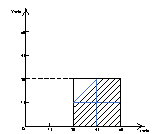
\includegraphics[width=9cm]{img/1.18.pdf}
\end{minipage}

\textcolor{themeColor}{\selectfont \ding{226} 几何概型.}
    \end{bbox}

\vspace{-5em}

    \begin{bbox}
    \begin{shaded}
        \qitem$^*$
(博雷尔-坎泰利(Borel-Cantelli)引理) 设\{$A_n,n \geq 1$\}为事件列. 事件$B_{n}=\bigcup\limits_{k=n}^{\infty}A_{k}$表示事件$A_{k}$,$A_{k+1}$,$\cdots$中至少有一个发生, 而事件$C=\bigcap\limits_{n=1}^{\infty}B_{n}$表示事件$B_{1}$,$B_{2}$,$\cdots$同时发生. 所以事件$C$表示事件$A_{n},n \geq 1$中有无穷个事件发生, 我们把事件$C$记为\{$A_{n}$, i.o.\}(i.o.是无限频繁(infinitely often)的缩写). 试证明如下的博雷尔-坎泰利引理. 对于事件列$A_{n},n \geq 1$,

(1) 如果$\sum\limits_{k=1}^{\infty}P(A_{k})<\infty$, 则$P(A_{n},\ \text{i.o.})=0$;

(2) 如果\{$A_{k},k \geq 1$\}相互独立, $\sum\limits_{k=1}^{\infty}P(A_{k})=\infty$, 那么$P(A_{n},\ \text{i.o.})=1$.

提示:

(1) 若$i<j$, 则事件$B_{i}\supset B_{j}$, 所以
$$P(A_{n},\ \text{i.o.})=\lim\limits_{n \to \infty}P(B_{n}),$$
再用不等式
$$P(\bigcup\limits_{k=n}^{\infty}A_{k}) \leq \sum\limits_{k=n}^{\infty}P(A_{k});$$

(2) 对$0 < x < 1$, 利用不等式$\ln(1-x) > -x$.
    \end{shaded}
    \end{bbox}

\vspace{-5em}

    \begin{bbox}
解: 

先说明一下上下限事件的定义: 

$\{A_{n}\}$的上限事件: 
$$\limsup\limits_{n\to\infty}A_{n}=\bigcap\limits_{n=1}^{\infty}\bigcup\limits_{m=n}^{\infty}A_{m},$$
它表示$A_{n}$发生无穷多次, 因为$\omega\in RHS$ $\Longleftrightarrow$ $\omega$属于无穷多个$A_{n}$, 记
$$\{A_{n},i.o.\}=\limsup\limits_{n\to\infty}A_{n}$$
$\{A_{n}\}$的下限事件: 
$$\liminf\limits_{n\to\infty}A_{n}=\bigcup\limits_{n=1}^{\infty}\bigcap\limits_{m=n}^{\infty}A_{m},$$
它表示$A_{n}$至多只有有限个不发生, $\omega\in RHS$ $\Longleftrightarrow$ $\exists n\in \mathbb{N}$, s.t. $\omega\in\bigcap\limits_{m=n}^{\infty}A_{m}$.

    \end{bbox}

\vspace{-5em}

    \begin{bbox}

下面是Borel-Cantelli引理的证明:

设$A = \bigcap\limits_{n=1}^{\infty}\bigcup\limits_{m=n}^{\infty} A_m$. 对第一部分(1)

\[
\mathbb{P}(A) \leq \mathbb{P}\left( \bigcup_{m=n}^{\infty} A_m \right) \leq \sum_{m=-n}^{\infty} \mathbb{P}(A_m) \to 0.
\]

对第二部分(2), 由(1)知$\Leftarrow$. 另一方面, 只需 $\mathbb{P}(A^c) = 0$. 而

\[
A^c = \bigcup_{n=1}^{\infty} \bigcap_{m=n}^{\infty} A_m^c,
\]

所以

\[
\mathbb{P}\left( \bigcap_{m=n}^{\infty} A_m^c \right) = \lim_{r \to \infty} \mathbb{P}\left( \bigcap_{m=n}^{r} A_m^c \right) \xlongequal{\text{独立性}} \lim_{r \to \infty} \prod_{m=n}^{r} \left( 1 - \mathbb{P}(A_m) \right) \leq e^{-\sum_{m=n}^{\infty} \mathbb{P}(A_m)} = 0.
\]

因此 $\mathbb{P}(A^c) = 0$.

\textcolor{themeColor}{\selectfont \ding{226} 这部分直接照搬刘党政老师的《简明概率论》讲义.}

\textcolor{themeColor}{\selectfont \ding{226} (1)的本质是实分析中的Borel-Cantelli引理:\\
设$(X,\Gamma,\mu)$是测度空间, $A_{n}\in\Gamma(\forall n)$. 则
$$\sum\limits_{n=1}^{\infty}\mu(A_{n}) < \infty \Longrightarrow \mu(\varlimsup\limits_{n\to\infty})=0.$$}
    \end{bbox}

\vspace{-5em}

    \begin{bbox}
    \begin{shaded}
        \qitem$^*$
如果把$P(A|B) > P(A)$理解为“$B$对$A$有促进作用”, 那么直观上似乎能有如下的结论: 由$P(A|B) > P(A)$及$P(B|C) > P(B)$推出$P(A|C) > P(A)$(意思是$B$促进了$A$, $C$促进了$B$, 故$C$促进了$A$). 举一简例说明上述直观看法不对.
    \end{shaded}
    \end{bbox}

\vspace{-5em}

    \begin{bbox}
解: 

记$A$: 骰子点数为4或6, $B$: 骰子点数为2或4, $C$: 骰子点数为1, 2或4. 则有: $P(A)=\frac{1}{3}$, $P(B)=\frac{1}{3}$, $P(C)=\frac{1}{2}$, $P(A|B)=\frac{1}{2}$, $P(B|C)=\frac{2}{3}$, $P(A|C)=\frac{1}{3}$, 满足$P(A|B)>P(A)$, $P(B|C)>P(B)$但$P(A|C)=P(A)$.

\textcolor{themeColor}{\selectfont \ding{226} 本质是条件概率不存在传递性.}
    \end{bbox}

\vspace{-5em}

    \begin{bbox}
    \begin{shaded}
        \qitem
考虑一元二次方程 $x^{2} + Bx + C = 0$, 其中$B$,$C$分别是将一枚均匀骰子连掷两次先后出现的点数. 求该方程有实根的概率和有重根的概率.
    \end{shaded}
    \end{bbox}

\vspace{-5em}

    \begin{bbox}
解: 

根据判别式$\Delta=B^2-4C,(B,C)\in\{1,2,3,4,5,6\}^2$, 穷举即可, 结果为$p_{\text{实}}=\frac{19}{36}$, $p_{\text{重}}=\frac{1}{18}$.
    \end{bbox}

\vspace{-5em}

    \begin{bbox}
    \begin{shaded}
        \qitem
某路公交汽车共有$11$个停车站, 由始发站开车时车上共有8名乘客. 假设每人在各站(始发站除外)下车的概率相同. 试求下列各事件发生的概率:

(1) 8人在不同的车站下车;

(2) 8人在同一车站下车;

(3) 8人中恰有3人在终点站下车.
    \end{shaded}
    \end{bbox}

\vspace{-5em}

    \begin{bbox}
解: 

(1) $p_{1}=\frac{A_{10}^{8}}{10^8}\approx0.018$.

(2) $p_{2}=\frac{10}{10^8}=1\times10^{-7}$.

(3) $p_{3}=\frac{\binom{8}{3}\cdot 9^5}{10^8}\approx0.033$
    \end{bbox}

\vspace{-5em}

    \begin{bbox}
    \begin{shaded}
        \qitem$^{*}$
设某地有$n + 1$个微信群, 某个造谣者向第二个微信群转发了谣言, 而第二个微信群中有人向第三个微信群转发该谣言, 如此下去. 在每一步中, 谣言的接收群都是随机从其余 n 个微信群中选取的.

(1) 求谣言传播了$r$次后还没有回到第一个造谣者所在的群的概率;

(2) 求没有一个微信群两次收到谣言的概率;

(3) 若每次随机地向$m$个微信群传播谣言, 回答上面两个问题.
    \end{shaded}
    \end{bbox}

\vspace{-5em}

    \begin{bbox}
解: 

(这类题似乎倾向于将造谣者转发的过程定义为造谣, 后面的才算传播, 但我个人还是将造谣者转发的过程也定义为传播, 总之不影响对知识点的掌握.)

(1) $p_{1}=(\frac{n-1}{n})^{r-1}$.

(2) $p_{2}=\frac{A_{n}^{r}}{n^r}=\frac{n!}{(n-r)!n^r}$.

(3.1) $p_{1}'=(\frac{\binom{n-1}{m}}{\binom{n}{m}})^{r-1}=(\frac{n-m}{n})^{r-1}$.

(3.2) 先在$n$个群中选取$rm$个不同的群, 有$\binom{n}{rm}$种选择, 再将这些群分配到$r$步, 分配方式有$\frac{(rm)!}{(m!)^{r}}$种. 故$p_{2}'=\displaystyle\frac{\binom{n}{rm}\frac{(rm)!}{(m!)^{r}}}{[\binom{n}{m}]^{r}}=\frac{[(n-m)!]^{r}}{(n!)^r(n-rm)!}$.
    \end{bbox}

\vspace{-5em}

    \begin{bbox}
    \begin{shaded}
        \qitem
有两箱同种类型的零件. 第一箱装50只, 其中10只为一等品; 第二箱装30只, 其中18只为一等品. 今从两箱中任挑出一箱, 然后从该箱中取零件两次, 每次任取一只, 做不放回抽样. 试求:

(1) 第一次取到的零件是一等品的概率;

(2) 在第一次取到的零件是一等品的条件下, 第二次取到的也是一等品的概率.
    \end{shaded}
    \end{bbox}

\vspace{-5em}

    \begin{bbox}
解: 

(1) 记挑到第一箱为事件$A$, 第$i$次$(i=1,2)$取到的零件是一等品为事件$B_{i}$, 则由全概率公式:
$$P(B_{1})=P(B_{1}|A)P(A)+P(B_{1}|\overline{A})P(\overline{A})=0.4.$$
(2)

\ding{172} $P(B_{2}|B_{1})=\frac{P(B_{1}B_{2})}{P(B_{1})}$, 同样由全概率公式:
$$P(B_{1}B_{2})=P(B_{1}B_{2}|A)P(A)+P(B_{1}B_{2}|\overline{A})P(\overline{A}),$$
其中$P(B_{1}B_{2}|A)=\frac{10}{50}\times\frac{9}{49}$, $P(B_{1}B_{2}|\overline{A})=\frac{18}{30}\times\frac{17}{29}$ $\Longrightarrow$ $P(B_{2}|B_{1})=\frac{690}{1421}\approx0.4856$.

\ding{173} 由贝叶斯公式:
$$P(A|B_{1})=\frac{P(B_{1}|A)P(A)}{P(B_{1})}=\frac{1}{4}\qquad P(\overline{A}|B_{1})=1-P(A|B_{1})=\frac{3}{4},$$
再由$P(B_{2}|B_{1})=P(B_{2}|AB_{1})P(A|B_{1})+P(B_{2}|\overline{A}B_{1})P(\overline{A}|B_{1})$, 其中$P(B_{2}|AB_{1})=\frac{9}{49}$, $P(B_{2}|\overline{A}B_{1})=\frac{17}{29}$ $\Longrightarrow$ $P(B_{2}|B_{1})=\frac{690}{1421}\approx0.4856$.

\textcolor{themeColor}{\selectfont \ding{226} 全概率公式; 贝叶斯公式.}
    \end{bbox}

\vspace{-5em}

    \begin{bbox}
    \begin{shaded}
        \qitem
设笔袋中有$r$支红色铅笔、$b$支黑色铅笔. 每次从袋中任取一支笔, 观察其颜色后放回, 并再加入$a$支同色的铅笔. 求第一次、第二次取到红色铅笔且第三次、第四次取到黑色铅笔的概率.
    \end{shaded}
    \end{bbox}

\vspace{-5em}

    \begin{bbox}
解: 

记第$i$次$(i \geq 1)$取到红色铅笔为事件$A_{i}$, 则:
$$P(A_{1}A_{2}\mathop{\overline{A_{3}}}\mathop{\overline{A_{4}}})=P(A_{1})P(A_{2}|A_{1})P(\overline{A_{3}}|A_{1}A_{2})P(\overline{A_{4}}|A_{1}A_{2}A_{3})=\frac{b(a+b)r(r+a)}{(r+b)(r+a+b)(r+2a+b)(r+3a+b)}.$$
    \end{bbox}

\vspace{-5em}

    \begin{bbox}
    \begin{shaded}
        \qitem
某工厂的一、二、三号车间生产同一种产品, 产量各占总产量的1/2, 1/3, 1/6, 次品率分别为1\%, 1\%, 2\%. 现从该厂随机抽取一件产品.

(1) 求该产品是次品的概率;

(2) 若发现该产品是次品, 求它是一号车间生产的概率.
    \end{shaded}
    \end{bbox}

\vspace{-5em}

    \begin{bbox}
解: 

记该产品是次品为事件$A$, 该产品是由一、二、三号车间生产的分别为事件$B_{i},1 \leq i \leq 3$.

(1) 由全概率公式:
$$P(A)=P(A|B_{1})P(B_{1})+P(A|B_{2})P(B_{2})+P(A|B_{3})P(B_{3})=\frac{7}{600}.$$
(2) 由贝叶斯公式:
$$P(B_{1}|A)=\frac{P(A|B_{1})P(B_{1})}{P(A)}=\frac{3}{7}.$$

\textcolor{themeColor}{\selectfont \ding{226} 全概率公式; 贝叶斯公式.}
    \end{bbox}

\vspace{-5em}

    \begin{bbox}
    \begin{shaded}
        \qitem
设男性色盲的概率为0.05, 女性色盲的概率为0.0025, 现发现从人群中任选的一人为色盲患者, 求此人为男性的概率.
    \end{shaded}
    \end{bbox}

\vspace{-5em}

    \begin{bbox}
解: 

设该人是男性为事件$A$, 该人是色盲患者为事件$B$. 由贝叶斯公式:
$$P(A|B)=\frac{P(B|A)P(A)}{P(B|A)P(A)+P(B|\overline{A})P(\overline{A})}=\frac{20}{21}\approx0.9524.$$

\textcolor{themeColor}{\selectfont \ding{226} 贝叶斯公式.}
    \end{bbox}

\vspace{-5em}

    \begin{bbox}
    \begin{shaded}
        \qitem
设有来自三个地区的考生报名表共50份, 三个地区分别有10份、15份和25份, 其中女生报名表分别为3份、7份和5份, 现随机地选一个地区, 从该地区的报名表中先后抽出2份.

(1) 求先抽到的1份是女生报名表的概率;

(2) 已知后抽到的1份是男生报名表, 求先抽到的1份是女生报名表的概率.
    \end{shaded}
    \end{bbox}

\vspace{-5em}

    \begin{bbox}
解: 

设选择第$i$个地区为事件$A_{i},1 \leq i \leq 3$, 第$j$次抽到女生为事件$B_{j},1 \leq i \leq 2$.

(1) 由全概率公式:
$$P(B_{1})=P(B_{1}|A_{1})P(A_{1})+P(B_{1}|A_{2})P(A_{2})+P(B_{1}|A_{3})P(A_{3})=\frac{29}{90}\approx0.322.$$

(2) 同样由全概率公式:
$$P(B_{1}|\overline{B_{2}})=\frac{P(B_{1}\overline{B_{2}})}{P(\overline{B_{2}})}=\frac{\sum\limits_{i=1}^{3}P(B_{1}\overline{B_{2}}|A_{i})P(A_{i})}{\sum\limits_{i=1}^{3}P(\overline{B_{2}}|A_{i})P(A_{i})},$$
其中对于不放回随机抽样, 第二次抽到男生的概率与第一次相等, 故$P(\overline{B_{2}}|A_{1})=\frac{7}{10}$, $P(\overline{B_{2}}|A_{2})=\frac{8}{15}$, $P(\overline{B_{2}}|A_{3})=\frac{4}{5}$ $\Longrightarrow$ $P(B_{1}|\overline{B_{2}})=\frac{20}{61}\approx0.328$.

\textcolor{themeColor}{\selectfont \ding{226} 全概率公式, 不放回随机抽样的性质.}
    \end{bbox}

\vspace{-5em}

    \begin{bbox}
    \begin{shaded}
        \qitem
罐子中有25个球, 其中20个红球、5个黑球, 从中不放回取出5个球, 不看颜色直接扔掉, 然后再从剩下的球中随机摸出一球发现是红球, 求扔掉的球里至少有两个红球的概率.
    \end{shaded}
    \end{bbox}

\vspace{-5em}

    \begin{bbox}
解: 

设扔掉的球中红球的数量为随机变量$X$, 记从剩下的20个球中摸到红球为事件$A$. 则由贝叶斯公式:
$$P(X\geq2|A)=\frac{\sum\limits_{i=2}^{5}P(A|X=i)P(X=i)}{\sum\limits_{i=0}^{5}P(A|X=i)P(X=i)},$$
其中$P(X=i)=\displaystyle\frac{\binom{20}{i}\binom{5}{5-k}}{\binom{25}{5}}$ $\Rightarrow$ $P(X\geq2|A)=\frac{1767}{1771}\approx0.9977.$

\textcolor{themeColor}{\selectfont \ding{226} 贝叶斯公式; 这里的$X$服从的是参数为(N=25, M=20, n=5)的超几何分布(Hypergeometric Distribution), 即$X\sim H(25,20,5)$.}
    \end{bbox}

\vspace{-5em}

    \begin{bbox}
    \begin{shaded}
        \qitem
假定某种病菌在群体中的带菌率为10\%. 在检测时, 带菌者和不带菌者被检测出阳性的
概率分别为0.95和0.01.

(1) 现有某人被测出呈阳性反应, 该人确为带菌者的概率是多少?

(2)$^*$  上一问中的人又独立地做了一次检测, 检测结果依然是阳性, 问在两次检测均呈阳性的情况下, 该人确为带菌者的概率是多少?
    \end{shaded}
    \end{bbox}

\vspace{-5em}

    \begin{bbox}
解: 

记该人确为带菌者为事件$A$, 该人第$i$次($1 \leq i \leq 2$)检测呈阳性为事件$B_{i}$.

(1) 由贝叶斯公式:
$$P(A|B_{1})=\frac{P(B_{1}|A)P(A)}{P(B_{1}|A)P(A)+P(B_{1}|\overline{A})P(\overline{A})}=\frac{95}{104}\approx0.91$$

(2) 由两次检测的独立性:
$$P(A|B_{1}B_{2})=\frac{P(B_{1}B_{2}|A)P(A)}{P(B_{1}B_{2}|A)P(A)+P(B_{1}B_{2}|\overline{A})P(\overline{A})}=\frac{9025}{9034}\approx0.999.$$

\textcolor{themeColor}{\selectfont \ding{226} 贝叶斯公式.}
    \end{bbox}

\vspace{-5em}

    \begin{bbox}
    \begin{shaded}
        \qitem
桌上有3个笔筒, 第1个笔筒装有2支红芯圆珠笔、4支蓝芯圆珠笔; 第2个笔筒装有4支红芯圆珠笔、2支蓝芯圆珠笔; 第3个笔筒装有3支红芯圆珠笔、3支蓝芯圆珠笔. 笔筒外表看起来一模一样, 先随机取一个笔筒, 任取一支笔出来.

(1) 试求取得红芯圆珠笔的概率;

(2) 在已知取得红芯圆珠笔的条件下, 问笔从哪个笔筒中取出的概率最大?
    \end{shaded}
    \end{bbox}

\vspace{-5em}

    \begin{bbox}
解: 

记选取第$i$个笔筒为事件$A_{i},1 \leq i \leq 3$, 取到红芯圆珠笔为事件$B$.

(1) 由全概率公式:
$$P(B)=P(B|A_{1})P(A_{1})+P(B|A_{2})P(A_{2})+P(B|A_{3})P(A_{3})=\frac{1}{2}.$$

(2) 由贝叶斯公式:
$$P(A_{i}|B)=\frac{P(B|A_{i})P(A_{i})}{P(B|A_{1})P(A_{1})+P(B|A_{2})P(A_{2})+P(B|A_{3})P(A_{3})}.$$
$\Longrightarrow$ $P(A_{1}|B)=\frac{2}{9}$, $P(A_{2}|B)=\frac{4}{9}$, $P(A_{3}|B)=\frac{1}{3}$ $\Longrightarrow$ 笔从第二个笔筒取出的可能性最大.

\textcolor{themeColor}{\selectfont \ding{226} 全概率公式; 贝叶斯公式.}
    \end{bbox}

\vspace{-5em}

    \begin{bbox}
    \begin{shaded}
        \qitem
计算机信号“0”和“1”传递出去, 信息站接收的时候, 0被误收为1的概率为0.02, 1被误收为0的概率为0.01. 信号0和1传输的频繁程度为2:1. 若接收到的信号是0, 则真实信号是0的概率是多少?
    \end{shaded}
    \end{bbox}

\vspace{-5em}

    \begin{bbox}
解: 

记真实信号是0为事件$A$, 接收到的信号是0为事件$B$. 由贝叶斯公式:
$$P(A|B)=\frac{P(B|A)P(A)}{P(B|A)P(A)+P(B|\overline{A})P(\overline{A})}=\frac{196}{197}\approx0.995.$$

\textcolor{themeColor}{\selectfont \ding{226} 贝叶斯公式.}
    \end{bbox}

\vspace{-5em}

    \begin{bbox}
    \begin{shaded}
        \qitem
有甲、乙两只口袋, 甲袋中有5只白球和2只黑球, 乙袋中有4只白球和5只黑球. 先从甲袋中任取两球放入乙袋, 然后再从乙袋中任取一球.
(1) 求从乙袋中取出的球为白球的概率;
(2) 若已知从乙袋中取出的球为白球, 求从甲袋中取的两球中有白球的概率.
    \end{shaded}
    \end{bbox}

\vspace{-5em}

    \begin{bbox}
解:

记从甲袋放入乙袋的球中白球的数量为随机变量$X$, 取出从乙袋中取出的球是白球为事件$A$.

(1) 由全概率公式:
$$P(A)=\sum\limits_{i=0}^{2}P(A|X=i)P(X=i)=\frac{38}{77}\approx0.49.$$

(2) 由贝叶斯公式:
$$P(X\geq1|A)=\frac{\sum\limits_{i=1}^{2}P(A|X=i)P(X=i)}{\sum\limits_{i=0}^{2}P(A|X=i)P(X=i)}=\frac{55}{57}\approx0.96.$$

\textcolor{themeColor}{\selectfont \ding{226} 全概率公式; 贝叶斯公式.}
    \end{bbox}

\vspace{-5em}

    \begin{bbox}
    \begin{shaded}
        \qitem
证明: 若$P(B|A) = P(B|\mathop{\overline{A}})$, 则事件$A$与$B$独立.
    \end{shaded}
    \end{bbox}

\vspace{-5em}

    \begin{bbox}
解:
$$P(B|A) = P(B|\mathop{\overline{A}}) \Longleftrightarrow \frac{P(AB)}{P(A)}=\frac{P(\overline{A}B)}{P(\overline{A})}=\frac{P(B)-P(AB)}{1-P(A)} \Longleftrightarrow P(AB)=P(A)P(B) \Longleftrightarrow A,B\text{独立}.$$
    \end{bbox}

\vspace{-5em}

    \begin{bbox}
    \begin{shaded}
        \qitem
如果$P(B|A) > P(B)$, 那么称$A$倾向于$B$. 证明: 如果$A$倾向于$B$, 那么$\overline{A}$也倾向于$\overline{B}$.
    \end{shaded}
    \end{bbox}

\vspace{-5em}

    \begin{bbox}
解: 

$$P(B|A) > P(B) \Longleftrightarrow P(AB) > P(A)P(B) \Longleftrightarrow P(\overline{A}B) < P(\overline{A})P(B) \Longleftrightarrow P(\mathop{\overline{A}}\mathop{\overline{B}}) > P(\mathop{\overline{A}})P(\mathop{\overline{B}}).$$
    \end{bbox}

\vspace{-5em}

    \begin{bbox}
\textcolor{themeColor}{\selectfont \ding{226} 与证明过程一致, 由于$\overline{\overline{A}}=A$, 这道题的逆命题也是成立的.}
    \end{bbox}

\vspace{-5em}

    \begin{bbox}
    \begin{shaded}
        \qitem
事件$A$与事件$B$至少发生一个的概率是0.12, 同时发生的概率是0.1, 请问事件$A$与事件$B$相互独立吗?
    \end{shaded}
    \end{bbox}

\vspace{-5em}

    \begin{bbox}
解:

$P(A)+P(B)=P(A\cup B)+P(A\cap B)=0.22$, 反证法: 设$A,B$相互独立, 则$P(A)P(B)=P(A\cap B)=0.1$ $\Longrightarrow$ $\left(P(A)-P(B)\right)^2=\left(P(A)+P(B)\right)^2-4P(A)P(B)=-0.3516$矛盾. 故$A,B$不相互独立.

\textcolor{themeColor}{\selectfont \ding{226} 本质是韦达定理.}
    \end{bbox}

\vspace{-5em}

    \begin{bbox}
    \begin{shaded}
        \qitem
对于三个事件$A$,$B$,$C$, 若
$$P(AB|C)=P(A|C)P(B|C)$$
成立, 则称$A$与$B$关于$C$条件独立. 若已知$A$与$B$关于$C$与$\overline{C}$条件独立, 且$P(C)=0.5$, $P(A|C)=P(B|C)=0.9$, $P(A|\overline{C})=0.2$, $P(B|\overline{C})=0.1$, 试求$P(A)$, $P(B)$, $P(AB)$, 并证明$A$与$B$不相互独立.
    \end{shaded}
    \end{bbox}

\vspace{-5em}

    \begin{bbox}
解:

由全概率公式:
$$P(A)=P(A|C)P(C)+P(A|\overline{C})P(\overline{C})=0.55,\qquad P(B)=P(B|C)P(C)+P(B|\overline{C})P(\overline{C})=0.5,$$
$A$与$B$关于$C$与$\overline{C}$条件独立 $\Longrightarrow$
$$P(AB)=P(AB|C)P(C)+P(AB|\overline{C})P(\overline{C})=P(A|C)P(B|C)P(C)+P(A|\overline{C})P(B|\overline{C})P(\overline{C})=0.415.$$
$$P(A)P(B) \neq P(AB) \Longrightarrow A\text{与}B\text{不相互独立}$$
    \end{bbox}

\vspace{-5em}

    \begin{bbox}
    \begin{shaded}
        \qitem
对于同一目标进行三次独立射击 第一、二、三次射中的命中率分别为0.5, 0.6和0.8, 试求:

(1) 在这三次射击中, 恰好有一次射中的概率;

(2) 在这三次射击中, 至少射中一次的概率.
    \end{shaded}
    \end{bbox}

\vspace{-5em}

    \begin{bbox}
解:

记第$i$次$(i=1,2,3)$射中为事件$A_{i}$, 则:

(1) 由独立性:
$$p_{1}=P(A_{1}\mathop{\overline{A_{2}}}\mathop{\overline{A_{3}}})+P(\mathop{\overline{A_{1}}}A_{2}\mathop{\overline{A_{3}}})+P(\mathop{\overline{A_{1}}}\mathop{\overline{A_{2}}}A_{3})=0.26.$$

(2) $$p_{2}=1-P(\mathop{\overline{A_{1}}}\mathop{\overline{A_{2}}}\mathop{\overline{A_{3}}})=0.96.$$
    \end{bbox}

\vspace{-5em}

    \begin{bbox}
    \begin{shaded}
        \qitem
求下列图中各系统能正常工作的概率, 其中框图中的字母代表元件, 字母相同但下标不同的都是同一种元件, 只是装配在不同的位置上, 元件$A$, $B$, $C$, $D$能正常工作的概率分别为$p_A$, $p_B$, $p_C$, $p_D$.

\begin{minipage}{9cm}
    \centering
    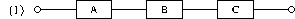
\includegraphics[width=9cm]{img/1.39_1.pdf}
\end{minipage}

\vspace{1em}

\begin{minipage}{6cm}
    \centering
    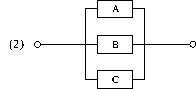
\includegraphics[width=6cm]{img/1.39_2.pdf}
\end{minipage}

\vspace{1em}

\begin{minipage}{8cm}
    \centering
    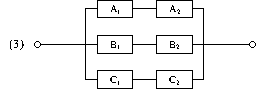
\includegraphics[width=8cm]{img/1.39_3.pdf}
\end{minipage}

\vspace{1em}

\begin{minipage}{8cm}
    \centering
    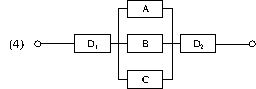
\includegraphics[width=8cm]{img/1.39_4.pdf}
\end{minipage}

\vspace{1em}

\begin{minipage}{8cm}
    \centering
    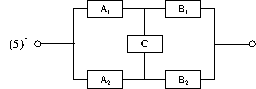
\includegraphics[width=8cm]{img/1.39_5.pdf}
\end{minipage}
    \end{shaded}
    \end{bbox}

\vspace{-5em}

    \begin{bbox}
解: 

(1) $p_{1}=p_{A}p_{B}p_{C}$.

(2) $p_{2}=1-(1-p_{A})(1-p_{B})(1-p_{C})$.

(3) $p_{3}=1-(1-p_{A}^2)(1-p_{B}^2)(1-p_{C}^2)$.

(4) $p_{4}=p_{D}^2[1-(1-p_{A})(1-p_{B})(1-p_{C})]$.

(5) 该图共有四条通路: $A_{1}\longrightarrow B_{1}$; $A_{2}\longrightarrow B_{2}$; $A_{1}\longrightarrow C\longrightarrow B_{2}$; $A_{2}\longrightarrow C\longrightarrow B_{1}$. 

\ding{172} 记该四条通路连通分别为事件$M_{i},1 \leq i \leq 4$. 则: $P(M_{1})=P(M_{2})=p_{A}p_{B}$, $P(M_{3})=P(M_{4})=p_{A}p_{B}p_{C}$, $P(M_{1}M_{2})=p_{A}^2 p_{B}^2$, $P(M_{1}M_{3})=P(M_{2}M_{4})=p_{A}p_{B}^2 P_{C}$, $P(M_{1}M_{4})=P(M_{2}M_{3})=p_{A}^2 p_{B}p_{C}$, $P(M_{3}M_{4})=p_{A}^2 p_{B}^2 p_{C}$, $P(M_{i}M_{j}M_{k})=p_{A}^2 p_{B}^2 p_{C}, \forall 1\leq i,j,k\leq 4=P(M_{1}M_{2}M_{3}M_{4})$. 由容斥原理: 
$$p_{5}=P(\bigcup\limits_{i=1}^{4}M_{i})=\sum\limits_{k=1}^{4}(-1)^{k-1}\sum\limits_{1\leq i_{1}<\cdots<i_{k}\leq 4}P(M_{i_{1}}\cap M_{i_{2}}\cdots\cap M_{i_{k}})=2p_{A}p_{B}[1+p_{C}(1-p_{A})(1-p_{B})]-p_{A}^2 p_{B}^2.$$
\ding{173} 记$K_{i}$为$K_{i}$能正常工作($K\in\{A,B,C\},i\in\{\emptyset,1,2\}$).

$C$能正常工作时: 系统能正常工作$\Longleftrightarrow$ $A_{1}$, $A_{2}$至少有一个能正常工作且$B_{1}$, $B_{2}$至少有一个能正常工作, 即:
$$p_{5|C}=P(A_{1}\cup A_{2})P(B_{1}\cup B_{2})=[1-(1-p_{A})^2][1-(1-p_{B})^2].$$
$C$不能正常工作时: 系统能正常工作$\Longleftrightarrow$ $A_{1}$, $B_{1}$能正常工作或$A_{2}$, $B_{2}$能正常工作, 即:
$$p_{5|\overline{C}}=1-(1-p_{A}p_{B})^2.$$
综上, 由全概率公式: 
$$p_{5}=p_{5|C}P(C)+p_{5|\overline{C}}P(\overline{C})=2p_{A}p_{B}[1+p_{C}(1-p_{A})(1-p_{B})]-p_{A}^2 p_{B}^2.$$
\textcolor{themeColor}{\selectfont \ding{226} 容斥原理; 全概率公式.}
    \end{bbox}

\vspace{-5em}

    \begin{bbox}
    \begin{shaded}
        \qitem
一个电路共有三个继电器, 当第一个继电器断开, 或者第二个、第三个同时断开时, 电路断开. 现设三个继电器断开的概率依次为0.3, 0.4, 0.6, 且三个继电器断开与否相互独立. 求电路断开的概率.
    \end{shaded}
    \end{bbox}

\vspace{-5em}

    \begin{bbox}
解: 
$$p=0.3+0.4\times0.6-0.3\times0.4\times0.6=0.468.$$
\textcolor{themeColor}{\selectfont \ding{226} 容斥原理.}
    \end{bbox}
\end{qitems}

%----------------------------------------------------%

\section{\kaishu{随机变量及其分布}}
%\autotitle[l]{自由标题}{\qanswerloc{10}}

\begin{qitems}
    \begin{bbox}
    \begin{shaded}
        \qitem
双色球是目前彩票中最受欢迎的玩法之一. 投注区分为红色球号码区和蓝色球号码区, 红色球号码区由1到33共33个号码组成, 蓝色球号码区由1到16共16个号码组成.投注时, 选择6个不同的红色球号码和1个蓝色球号码组成一注进行单式投注, 每注金额人民币2元. 设开奖时, 由系统随机指定6个不同的红色球号码和1个蓝色球号码. 若某单式投注中分别有\( i (0 \le i \le 6) \)个红色球号码和\( j (j = 0, 1) \)个蓝色球号码与指定号码相同, 则称该投注的形式为``\( i+j \)''. 最后所有奖项规则如下:
\begin{center}
%\renewcommand{\arraystretch}{1}
\setlength{\tabcolsep}{14pt}
\begin{tabular}{c|c|c|c|c|c|c}
\hline
等级 & 一等奖 & 二等奖 & 三等奖 & 四等奖 & 五等奖 & 六等奖 \\
\hline
形式 & 6+1 & 6+0 & 5+1 & 5+0, 4+1 & 4+0, 3+1 & 2+1, 1+1, 0+1 \\
\hline
\end{tabular}
\end{center}
(1) 试引入一个随机变量\( X \)来描述随机购买的一注单式投注的各种中奖等级情况, 并求它的分布律;

(2) 试用\( X \)取值的方式来表示某人花 2 元买一注后的下述事件:
\[
A = \{\text{中奖}\}, \quad B = \{\text{中一等奖或二等奖}\}
\]
并求出它们发生的概率.
    \end{shaded}
    \end{bbox}

\vspace{-5em}

    \begin{bbox}
解: 

记匹配$i$个红色球号码为事件$A_{i}$, 匹配蓝色球号码为事件$B$, 随机变量$X$为:
\begin{center}
%\renewcommand{\arraystretch}{1}
\setlength{\tabcolsep}{13pt}
\begin{tabular}{c|c|c|c|c|c|c|c}
\hline
等级 & 未获奖 & 一等奖 & 二等奖 & 三等奖 & 四等奖 & 五等奖 & 六等奖 \\
\hline
$X$ & 0 & 1 & 2 & 3 & 4 & 5 & 6 \\
\hline
\end{tabular}
\end{center}
则$P(A_{i})=\displaystyle\frac{\binom{6}{i}\binom{27}{6-i}}{\binom{33}{6}}$, $P(B)=\displaystyle\frac{1}{16}$.

(1) 显然各个不同的$A_{i}\cap B$(或$A_{i}\cap B^{c}$)交集为空且$A_{i}$, $B$(或$B^c$)相互独立, 故$P((A_{m}B_{1})\cup(A_{n}B_{2}))=P(A_{m}B_{1})+P(A_{n}B_{2})$, $B_{1},B_{2}=B\text{或}B^c$且$P(A_{i}B)=P(A_{i})P(B)$(或$P(A_{i}B^{c})=P(A_{i})P(B^{c})$). 计算可得$X$的分布律如下:
\begin{center}
%\renewcommand{\arraystretch}{1}
\setlength{\tabcolsep}{13pt}
\begin{tabular}{c|c|c|c|c|c|c|c}
\hline
$X$ & 0 & 1 & 2 & 3 & 4 & 5 & 6 \\
\hline
$P(X=x)$ & $\frac{16532100}{17721088}$ & $\frac{1}{17721088}$ & $\frac{15}{17721088}$ & $\frac{162}{17721088}$ & $\frac{7695}{17721088}$ & $\frac{137475}{17721088}$ & $\frac{1043640}{17721088}$ \\
\hline
\end{tabular}
\end{center}
(2) $A=\{X \neq 0\}$, $B=\{X=1\text{或}2\}$ $\Longrightarrow$ $P(A)=1-P(X=0)=\frac{1189988}{17721088}\approx0.0671$, $P(B)=P(X=1)+P(X=2)=\frac{16}{17721088}\approx9.03\times10^{-7}$.
    \end{bbox}

\vspace{-5em}

    \begin{bbox}
    \begin{shaded}
        \qitem
一位篮球运动员练习投篮 100 次, 且己知他前两次只投进了一次. 从第3球开始, 假设他每次投篮的命中率为其前面所投进球的比率(比如他前5次投进了4个球, 则第6次他的投篮命中率为4/5). 求他最终在这100次投篮中投进次数的分布律.
    \end{shaded}
    \end{bbox}

\vspace{-5em}

    \begin{bbox}
解: 

记$S_n$为$n$次投篮中投进的次数, 由数学归纳法:

已知$n=3$时, $P(S_{3}=1)=\frac{1}{2}=P(S_{3}=2)=\frac{1}{2}$. 设$P(S_{n-1}=k)=\frac{1}{n-2},\forall1 \leq k \leq n-2$, 则: 
$$P(S_{n}=k)=\frac{k-1}{n-1}P(S_{n-1}=k-1)+\left(1-\frac{k}{n-1}\right)P(S_{n-1}=k)=\frac{1}{n-1}. \qquad\qquad\qquad\qquad\qquad\qquad\qquad\qedsymbol$$
综上所述, $S_{100}$服从在$\{1,2,\cdots,99\}$的等可能分布, 即$P(S_{100}=k)=\frac{1}{99},\forall1 \leq k \leq 99.$

\textcolor{themeColor}{\selectfont \ding{226} 数学归纳法.}

\textcolor{themeColor}{\selectfont \ding{226} 这道题实际上是一个随机强化模型, 依据过去经验不断更新决策概率, 这里服从等可能分布的本质原因是初始条件的对偶性. 与之等价的数学模型: 将``命中''等效为``从箱中抽出红球'',``未命中''等效为``从箱中抽出蓝球'', 命中则投入一个红球, 未命中则投入一个蓝球.}
    \end{bbox}

\vspace{-5em}

    \begin{bbox}
    \begin{shaded}
        \qitem
某物流公司和某工厂约定用车将一箱货物按期无损地运到目的地, 可得佣金100元, 但若不按期则扣20元(即得佣金80元); 若货物有损坏则扣50元; 若货物不按期又有损坏则扣160元. 该物流公司按以往经验认为一箱货物按期无损地运到目的地有60\%的把握, 不按期到达但无损坏的占20\%, 按期到达但货物有损坏的占10\%, 货物不按期到达又有损坏的占10\%. 以$X$记该物流公司用车将一箱货物运到目的地后的毛利润. 试求$X$的分布律.
    \end{shaded}
    \end{bbox}

\vspace{-5em}

    \begin{bbox}
解: 

显然, $X$的分布律为: 
\begin{center}
%\renewcommand{\arraystretch}{1}
\setlength{\tabcolsep}{38pt}
\begin{tabular}{c|c|c|c|c}
\hline
$X$ & 100 & 80 & 50 & -60 \\
\hline
$P(X=x)$ & 0.6 & 0.2 & 0.1 & 0.1 \\
\hline
\end{tabular}
\end{center}
    \end{bbox}

\vspace{-5em}

    \begin{bbox}
    \begin{shaded}
        \qitem
设某游乐场的一部设备在一天内发生故障的概率为0.2, 设备一旦发生故障则全天无法工作. 若一周五个工作日内无故障可以获利10万元, 只发生一次故障可以获利5万元,发生两次故障获利0元, 发生三次或三次以上故障则亏损2万元. 试求一周内该游乐场在这台设备上的毛利润的分布律.
    \end{shaded}
    \end{bbox}

\vspace{-5em}

    \begin{bbox}
解: 

记五个工作日内发生故障的次数为随机变量$X$, 则$X$服从参数为$n=5$, $p=0.2$的二项分布, 即$X\sim B(5,0.2)$, 则$P(X=k)=\binom{5}{k}\cdot(0.2)^k\cdot(0.8)^{5-k}$, $0 \leq k \leq 5$. 故毛利润的分布律为:
\begin{center}
%\renewcommand{\arraystretch}{1}
\setlength{\tabcolsep}{26pt}
\begin{tabular}{c|c|c|c|c}
\hline
毛利润(万元) & 10 & 5 & 0 & -2 \\
\hline
$X$ & 0 & 1 & 2 & 3, 4, 5 \\
\hline
$P$ & 0.32768 & 0.4096 & 0.2048 & 0.05792 \\
\hline
\end{tabular}
\end{center}
\textcolor{themeColor}{\selectfont \ding{226} 二项分布.}
    \end{bbox}

\vspace{-5em}

    \begin{bbox}
    \begin{shaded}
        \qitem
设随机变量$X$的分布律如下: 
\begin{center}
%\renewcommand{\arraystretch}{1}
\setlength{\tabcolsep}{30pt}
\begin{tabular}{c|ccc}
$X$ & -1 & 1 & 2\\
\hline
$P$ & 0.25 & 0.5 & 0.25\\
\end{tabular}
\end{center}
(1) 试求$X$的分布函数$F(x)$;

(2) 试求概率$P(X \leq 0)$, $P(0.5 < X  \leq 1.5)$, $P(1 \leq X \leq 2)$和$P(1 < X \leq 2)$.
    \end{shaded}
    \end{bbox}

\vspace{-5em}

    \begin{bbox}
解: 

(1)
\vspace{-2em}
\begin{center}
\begin{equation}
    F(x)=
    \left\{
    \begin{array}{cl}
        \nonumber
        0,\ &x < -1,\\
        0.25,\ &-1 \leq x < 1,\\
        0.75,\ &1 \leq x < 2,\\
        1,\ &x \geq 2.
    \end{array}
    \right.
\end{equation}
\end{center}
(2) $P(X \leq 0)=F(0)=0.25$, $P(0.5 < X  \leq 1.5)=F(1.5)-F(0.5)=0.5$, $P(1 \leq X \leq 2)=F(2)-F(1)+P(X=1)=0.75$, $P(1 < X \leq 2)=F(2)-F(1)==0.25$.
    \end{bbox}

\vspace{-5em}

    \begin{bbox}
    \begin{shaded}
        \qitem
设10件产品中有8件是正品, 2件是次品. 现每次不放回地抽取一件产品直到取到正品为止. 以$X$记抽取的次数, 试求$X$的分布律和分布函数.
    \end{shaded}
    \end{bbox}

\vspace{-5em}

    \begin{bbox}
解: 

显然$X$的分布律为:
\begin{center}
%\renewcommand{\arraystretch}{1}
\setlength{\tabcolsep}{30pt}
\begin{tabular}{c|c|c|c}
    \hline
    $X$ & 1 & 2 & 3 \\
    \hline
    $P$ & 0.8 & $\frac{8}{45}\approx0.1778$ & $\frac{1}{45}\approx0.0222$\\
    \hline
\end{tabular}
\end{center}
分布函数为:
\vspace{-2em}
\begin{center}
\begin{equation}
    F(x)=
    \left\{
    \begin{array}{cl}
        \nonumber
        0,\ &x < 1,\\
        \frac{4}{5},\ &1 \leq x < 2,\\
        \frac{44}{45},\ &2 \leq x < 3,\\
        1,\ &x \geq 3.
    \end{array}
    \right.
\end{equation}
\end{center}
    \end{bbox}

\vspace{-5em}

    \begin{bbox}
    \begin{shaded}
        \qitem
在一串独立试验中观察某事件$A$是否发生, 且假设每次$A$发生的概率都是0.4. 若以$X$表示$A$发生时的累计试验次数, 试求概率$P(X\text{为偶数})$和$P(X > 2)$.
    \end{shaded}
    \end{bbox}

\vspace{-5em}

    \begin{bbox}
解: 

$X$服从参数为$p$的几何分布, 即$X\sim Ge(p)$; $P(X=k)=(1-p)^{k-1}p$, $k=1,2,\cdots$, 其中$p=0.4$. 则:
$$P(X\text{为偶数})=\sum\limits_{k=1}^{\infty}P(X=2k)=\sum\limits_{k=1}^{\infty}(1-p)^{2k-1}p=\frac{1-p}{2-p};$$
$$P(X > 2)=1-P(X=1)-P(X=2)=(1-p)^2.$$
代入$p=0.4$, 得:
$$P(X\text{为偶数})=0.375,\qquad P(X > 2)=0.36.$$
\textcolor{themeColor}{\selectfont \ding{226} 几何分布.}
    \end{bbox}

\vspace{-5em}

    \begin{bbox}
    \begin{shaded}
        \qitem
向目标进行20次独立射击, 且假设每次射击的命中率为0.2. 若以$X$记命中的次数, 试求概率$P(X \geq 1)$及$X$最有可能的取值.
    \end{shaded}
    \end{bbox}

\vspace{-5em}

    \begin{bbox}
解: 

$X$服从参数为$n=20$, $p=0.2$的二项分布, 即$X\sim B(20,0.2)$; $P(X=k)=\binom{20}{k}\cdot(0.2)^k\cdot(0.8)^{20-k}$, $k=0,1,\cdots,20$. 则:
    \end{bbox}
    
\vspace{-5em}

    \begin{bbox}
$$P(X \geq 1)=1-P(X=0)\approx0.9885.$$
$X$最有可能的取值即二项分布的众数, 由对应公式\textcolor{themeColor}{(见注释)}可知:
$$X_{\text{众}}=\lfloor(n+1)p\rfloor=4.$$
\textcolor{themeColor}{\selectfont \ding{226} 二项分布的众数(高中人教版附录里似乎有提到接下来的公式, 这里再证一遍): 设$X\sim B(n,p)$, 则:
$$k_{\text{众}}=\lfloor(n+1)p\rfloor$$
证: $\displaystyle\frac{P(X=k+1)}{P(X=k)}=\frac{\binom{n}{k+1}p^{k+1}(1-p)^{n-k-1}}{\binom{n}{k}p^{k}(1-p)^{n-k}}=\frac{(n-k)p}{(k+1)(1-p)}$关于$k$单调递减, 故令$\displaystyle\frac{(n-k)p}{(k+1)(1-p)} \leq 1 \Longleftrightarrow k \geq (n+1)p-1$. 从而$k_{\text{众}}=\lfloor(n+1)p\rfloor$是最小的满足$\displaystyle\frac{P(X=k+1)}{P(X=k)} \leq 1$的整数(注意当$(n+1)p\in\mathbb{Z}$时, $\frac{P((n+1)p)}{P((n+1)p-1)}=1$, 即有两个众数: $(n+1)p$, $(n+1)p-1)$.} \textcolor{red}{(!!!考试时建议不要直接套公式, 而是按这种方式给出完整计算或证明(`・ω・´).)}
    \end{bbox}

\vspace{-5em}

    \begin{bbox}
    \begin{shaded}
        \qitem
进行4次独立试验, 在每次试验中结果$A$出现的概率均为0.3. 若$A$不出现, 则$B$也不出现; 若A只出现一次, 则B出现的概率是0.6; 若$A$出现至少两次, 则$B$出现的概率为1. 试求: (1) $B$会出现的概率; (2) 若己知$B$出现, 求$A$恰出现一次的概率.
    \end{shaded}
    \end{bbox}

\vspace{-5em}

    \begin{bbox}
解: 

记结果$A$出现的次数为随机变量$X$, 则$X\sim B(4,0.3)$, 即$P(X=k)=\binom{4}{k}\cdot(0.3)^k\cdot(0.7)^{4-k}$, $0 \leq k \leq 4$

(1) 由全概率公式:
$$P(B)=\sum\limits_{k=0}^{4}P(B|X=k)P(X=k)=0.59526.$$

(2) 由贝叶斯公式:
$$P(X=1|B)=\frac{P(B|X=1)P(X=1)}{P(B)}\approx0.4149.$$

\textcolor{themeColor}{\selectfont \ding{226} 全概率公式; 贝叶斯公式; 二项分布.}
    \end{bbox}

\vspace{-5em}

    \begin{bbox}
    \begin{shaded}
        \qitem
有两支篮球队进行友谊杯赛, 假定每一场甲乙两队获胜的概率分别是0.6和0.4, 且各场胜负情况相互独立. 如果规定先胜4场者为冠军, 求甲队经过$i(i=4,5,6,7)$场比赛而成为冠军的概率$p_{i}$. 再问: 与 ``三场两胜''制比较, 采取哪种赛制对乙队更有利?
    \end{shaded}
    \end{bbox}

\vspace{-5em}

    \begin{bbox}
解: 

记甲队胜四场比赛所需的场次为随机变量$X$, 则$X$服从参数为$r=4$, $p=0.6$的负二项分布(帕斯卡分布), 即$X\sim NB(4,0.6)$, 则:
$$P(X=i)=\binom{i-1}{4-1}\cdot(0.4)^{4}\cdot(0.6)^{i-4},i=4,5,6,7$$
\begin{center}
    $\Longrightarrow$
%\renewcommand{\arraystretch}{1}
\setlength{\tabcolsep}{20pt}
\begin{tabular}{c|c|c|c|c}
    \hline
    $i$ & 4 & 5 & 6 & 7 \\
    \hline
    $P$ & 0.1296 & 0.20736 & 0.20736 & 0.165888\\
    \hline
\end{tabular}
\end{center}
$p_{\text{乙},4}=1-\sum\limits_{i=4}^{7}P(X=i)=0.289792 < p_{\text{乙},2}=0.352$ $\Longrightarrow$``三局两胜制''对乙队更有利(原理同第一章第12题).
    \end{bbox}

\vspace{-5em}

    \begin{bbox}
    \begin{shaded}
        \qitem
有一种赌博, 规则如下: 赌徒先在1到6中押一个数字, 然后掷三个骰子, 若赌徒所押的数字出现$i$次, $i=1,2,3$, 则赌徒赢$i$元; 若其所押的数字没出现, 则输1元. 以随机变量$X$表示赌徒赌完一局后的收益, 试求它的分布律(假设这些骰子都是均匀的且掷出的点数相互独立).
    \end{shaded}
    \end{bbox}

\vspace{-5em}

    \begin{bbox}
解: 

记$Y$为三个骰子中押的数字出现的次数, 则$Y\sim B(3,\displaystyle\frac{1}{6})$, 即$P(Y=k)=\binom{3}{k}\cdot(\displaystyle\frac{1}{6})^{k}\cdot(\frac{5}{6})^{3-k}$, $k=0,1,2,3$. 则: $P(x)=P(Y),X=1,2,3$; $P(X=-1)=P(Y=0)$ $\Longrightarrow$ $X$的分布律为:
\begin{center}
\renewcommand{\arraystretch}{1.5}
\setlength{\tabcolsep}{20pt}
\begin{tabular}{c|c|c|c|c}
    \hline
    $X$ & -1 & 1 & 2 & 3 \\
    \hline
    $P$ & $\displaystyle\frac{125}{216}$ & $\displaystyle\frac{25}{72}$ & $\displaystyle\frac{5}{72}$ & $\displaystyle\frac{1}{216}$ \\
    \hline
\end{tabular}
\end{center}
\textcolor{themeColor}{\selectfont \ding{226} 二项分布.}
    \end{bbox}

\vspace{-5em}

    \begin{bbox}
    \begin{shaded}
        \qitem
设某种昆虫单只每次产卵的数量服从参数为$\lambda$的泊松分布, 而每个虫卵能孵出幼虫的概率均为$p(0 < p < 1)$且相互独立. 分别以$Y$和$Z$记一只昆虫一次产卵后幼虫的个数和未能孵出幼虫的虫卵的个数. 试问$Y$和$Z$分别服从什么分布? 它们是否相互独立?
    \end{shaded}
    \end{bbox}

\vspace{-5em}

    \begin{bbox}
解: 

设一只昆虫一次产卵的数量为随机变量$N$, 则$N\sim P(\lambda)$, 即$P(N=k)=\displaystyle\frac{\lambda^k}{k!}e^{-\lambda}$, $k=0,1,2,\cdots$. 此外, $Y|N=n\sim B(n,p)$, $Z|N=n\sim B(n,1-p)$ $\Longrightarrow$ 由全概率公式:
    \end{bbox}

\vspace{-5em}

    \begin{bbox}
\vspace{-2em}
\begin{center}
\begin{equation}
\begin{aligned}
    \nonumber
P(Y=k)=\sum\limits_{n=k}^{\infty}P(N=n)P(Y=k|N=n) & =\sum\limits_{n=k}^{\infty}\frac{\lambda^n}{n!}e^{-\lambda}\binom{n}{k}p^{k}(1-p)^{n-k}\\
 & =e^{-\lambda}\frac{p^k}{k!}\sum\limits_{n=k}^{\infty}\frac{\lambda^{n}(1-p)^{n-k}}{(n-k)!}\\
 & \xlongequal{m=n-k} e^{-\lambda}\frac{(\lambda p)^k}{k!}\sum\limits_{m=0}^{\infty}\frac{\lambda^{m}(1-p)^{m}}{m!} = e^{-\lambda p}\frac{(\lambda p)^{k}}{k!}.
\end{aligned}
\end{equation}
\end{center}
故$Y\sim P(\lambda p)$. 同理, $Z\sim P(\lambda(1-p))$.
再计算:
\vspace{-2em}
\begin{center}
\begin{equation}
\begin{aligned}
    \nonumber
P(Y=y,Z=z)=P(N=y+z)P(Y=y,Z=z|N=y+z)&=e^{-\lambda}\frac{\lambda^{y+z}}{(y+z)!}\binom{y+z}{y}p^y(1-p)^z\\
&=e^{-\lambda p}\frac{(\lambda p)^y}{y!}\cdot e^{-\lambda(1-p)}\frac{(\lambda(1-p))^z}{z!}\\
&=P(Y=y)P(Z=z)
\end{aligned}
\end{equation}
\end{center}
$\Longrightarrow$ $Y$, $Z$相互独立.

\textcolor{themeColor}{\selectfont \ding{226} 泊松分布; 二项分布.}
    \end{bbox}

\vspace{-5em}

    \begin{bbox}
    \begin{shaded}
        \qitem
一个系统包含了1000个零件, 各个零件是否出故障是相互独立的并且在一个月内出故障的概率为0.001. 试利用泊松分布求系统在一个月内正常运转(即没有零件出故障)的概率.
    \end{shaded}
    \end{bbox}

\vspace{-5em}

    \begin{bbox}
解: 

记$n$为零件数, $p$为出故障的概率, $X$为一个月内出故障的零件个数, 则$X\sim B(n=1000,p=0.001)$. 由于$n=1000\geq30$(或$n\geq100$)且$np=1 \leq 5$(或$np \leq 10$), 故可以使用``泊松逼近定理''进行估算: 令$\lambda=np=1$, 则$P(X=0)\approx\frac{\lambda^{0}}{0!}e^{-\lambda}=e^{-1}\approx0.3679$.

\textcolor{themeColor}{\selectfont \ding{226} 泊松逼近定理及其判断(使用)条件, 见课本P57 定理2.2及下方的正文.}
    \end{bbox}

\vspace{-5em}

    \begin{bbox}
    \begin{shaded}
        \qitem
保险公司的资料表明, 持某种人寿保险单的人在保险期内死亡的概率为0.02. 利用泊松分布, 试求在400份保单中最终至少赔付两份保单的概率. 结果精确到小数点后三位.
    \end{shaded}
    \end{bbox}

\vspace{-5em}

    \begin{bbox}
解: 

记$n$为保单数, $p$为保险期内死亡概率, $X$为需要赔付的保单数, 则$X\sim B(n=400,p=0.02)$. 由于$n=400\geq100$且$np=8 \leq 10$, 故可以使用``泊松逼近定理''进行估算: 令$\lambda=np=10$, 则$P(X \geq 2)=1-P(X=0)-P(X=1)\approx1-9e^{-8}\approx0.997$.

\textcolor{themeColor}{\selectfont \ding{226} 泊松逼近定理及其判断(使用)条件, 见课本P57 定理2.2及下方的正文.}
    \end{bbox}

\vspace{-5em}

    \begin{bbox}
    \begin{shaded}
        \qitem
某种数码传输系统每秒传送$5.12\times10^5$个字符(0或1), 由于会受到干扰, 传送中会出现误码, 即将0(或1)传送为1(或0). 若误码率为$10^{-7}$, 求在10 s内至少出现一个误码的概率. 在100s内呢? 结果精确到小数点后三位.
    \end{shaded}
    \end{bbox}

\vspace{-5em}

    \begin{bbox}
解: 

记$n_{i},i=1,2$为指定秒内出现的字符数, $p$为出现误码的概率, $X_{i},i=1,2$为指定秒内出现的误码数, 则$X_{1}\sim B(n_{1}=5.12\times10^{6},p=10^{-7})$. 由于$n_{1}=5.12\times10^{6}\geq30$(或$n_{1}\geq100$)且$n_{1}p=0.512 \leq 5$(或$n_{1}p \leq 10$), 故可以使用``泊松逼近定理''进行估算: 令$\lambda_{1}=n_{1}p=1$, 则$P(X_{1} \geq 1)=1-P(X_{2}=0)\approx1-e^{-\lambda_{1}}\approx0.401$. 同理可得: $P(X_{2})\approx0.994$.

\textcolor{themeColor}{\selectfont \ding{226} 泊松逼近定理及其判断(使用)条件, 见课本P57 定理2.2及下方的正文.}
    \end{bbox}

\vspace{-5em}

    \begin{bbox}
    \begin{shaded}
        \qitem
某航空公司知道预订航班的乘客有0.05的概率最终不会来搭乘, 为了盈利更多, 他们的政策是接受比实际座位更多的预订. 若一个恰有50个座位的航班一共被预订了52张票, 问最终出现无法满足所有乘客乘坐要求的情况的概率大约是多少? 结果精确到小数点后两位.
    \end{shaded}
    \end{bbox}

\vspace{-5em}

    \begin{bbox}
解: 

记$n$为预订的票数, $p$为乘客不来搭乘的概率, $X$为最终不来搭乘的乘客数量, 则$X\sim B(n=52,p=0.05)$. 由于$n=52\geq30$且$np=2.6 \leq 5$, 故可以使用``泊松逼近定理''进行估算: 令$\lambda=np=2.6$, 则$P(X \leq 1)\approx3.6e^{-2.6}\approx0.27$.

\textcolor{themeColor}{\selectfont \ding{226} 泊松逼近定理及其判断(使用)条件, 见课本P57 定理2.2及下方的正文.}
    \end{bbox}

\vspace{-5em}

    \begin{bbox}
    \begin{shaded}
        \qitem
假定有100万注彩票出售, 其中有100注有奖.

(1) 若一个人买了100注, 求其中奖的概率;

(2) 一个人买多少注, 才能保证有0.95的概率中奖?
    \end{shaded}
    \end{bbox}

\vspace{-5em}

    \begin{bbox}
解: 

(1) 记总彩票数为$N$, 有奖彩票数为$M$, 购买的彩票数为$n$, 中奖次数为$X$, 则实际上$X$服从超几何分布, 即$X\sim H(N,M,n)$. 但因为$1\times10^{6}\gg100$, 所以每次买完一张彩票后, 下一张彩票中奖的概率$p$几乎不变, 即可以将该问题近似为二项分布: 令$p=\frac{M}{N}=0.0001$ $\Longrightarrow$ $X\sim B(n=100,p=0.0001)$. 又因为$n=100\geq 30$且$np=0.01\ll5$, 由泊松逼近定理, $P(X \geq 1)=1-P(X=0)\approx1-e^{-0.01}=0.00995$.
    \end{bbox}

\vspace{-5em}

    \begin{bbox}
(2) 要使$1-e^{-n'p}\geq0.95$ $\Longleftrightarrow$ $n'\geq29957$. 经检验, 此时$\frac{n'}{N}=0.29957$仍处于较小水平且$n'p=2.9957 \leq 5$, 仍满足二项分布近似与泊松逼近的条件.

\textcolor{themeColor}{\selectfont \ding{226} 泊松逼近定理及其判断(使用)条件, 见课本P57 定理2.2及下方的正文.}

\textcolor{themeColor}{\selectfont \ding{226} 第二题也可以直接用二项分布的概率计算, 在处理不等式时对多项式取对数, 由于$p$较小, 再使用$\ln(1-p)=\approx-p$进行近似, 结果与泊松逼近一致, 因为这就是它的本质.}

\textcolor{themeColor}{\selectfont \ding{226} 关于超几何分布和二项分布何时能近似, 貌似书上并没有提到, 但这里仅从百分比来判断依旧是合理的. 实际上利用超几何分布进行精确计算得到的结果是29512注, 但由于做题不太可能要求短时间内计算那么庞大的组合数, 所以不需要用超几何分布.} 
    \end{bbox}

\vspace{-5em}

    \begin{bbox}
    \begin{shaded}
        \qitem
设随机变量$X$的分布函数为:
\vspace{-2em}
\begin{center}
\begin{equation}
    F(x)=
    \left\{
    \begin{array}{cl}
        \nonumber
        0,\ &x < 0,\\
        x/4,\ &0 \leq x < 1,\\
        1/2+(x-1)/4,\ &1 \leq x < 2,\\
        5/6,\ &2 \leq x <3,\\
        1,\ &x \geq 3.
    \end{array}
    \right.
\end{equation}
\end{center}
试求: (1) $P(X=k)$, $k=1,2,3$;\qquad(2) $P(1/2<x<3/2)$.
    \end{shaded}
    \end{bbox}

\vspace{-5em}

    \begin{bbox}
解: (注: $f(x^\mp)=\lim\limits_{y\to x^\mp}f(y)$指$f$在$x$处的左右极限.)

(1) $P(X=k)=F(k)-F(k^{-})$ $\Longrightarrow$ $P(X=1)=\frac{1}{4}$; $P(X=2)=\frac{1}{12}$; $P(X=3)=\frac{1}{6}$.

(2) $P(\frac{1}{2}<x<\frac{3}{2})=F(\frac{3}{2}^-)-F(\frac{1}{2})=\frac{1}{2}$.
    \end{bbox}

\vspace{-5em}

    \begin{bbox}
    \begin{shaded}
        \qitem
设随机变量$X$的分布函数为:
\vspace{-2em}
\begin{center}
\begin{equation}
    F(x)=
    \left\{
    \begin{array}{cl}
        \nonumber
        0,\ &x < -1,\\
        1/8,\ &x=-1,\\
        ax+b,\ &-1 < x < 1,\\
        1,\ &x \geq 1,
    \end{array}
    \right.
\end{equation}
\end{center}
且$P(X=1)=\displaystyle\frac{1}{4}$, 试求常数$a$和$b$的值.
    \end{shaded}
    \end{bbox}

\vspace{-5em}

    \begin{bbox}
解: (注: $f(x^\mp)=\lim\limits_{y\to x^\mp}f(y)$指$f$在$x$处的左右极限.)

$F(1^-)=a+b=F(1)-P(X=1)=\displaystyle\frac{3}{4}$, $F(-1^+)=-a+b=F(-1)=\displaystyle\frac{1}{8}$ $\Longrightarrow$ $a=\displaystyle\frac{5}{16}$, $b=\displaystyle\frac{7}{16}$.
    \end{bbox}

\vspace{-5em}

    \begin{bbox}
    \begin{shaded}
        \qitem
设随机变量$X$的密度函数为:
\vspace{-2em}
\begin{center}
\begin{equation}
    f(x)=
    \left\{
    \begin{array}{cl}
        \nonumber
        ax,\ &1 < x < 2,\\
        b,\ &2 \leq x < 3,\\
        0,\ &\text{其他}.
    \end{array}
    \right.
\end{equation}
\end{center}
若又知$P(1 < X <2)=P(2 < X < 3)$, 试求常数$a$和$b$的值.
    \end{shaded}
    \end{bbox}

\vspace{-5em}

    \begin{bbox}
解:

$\displaystyle P(1 < x < 2)=\int_{1}^{2}ax \mathrm{d}x=\int_{2}^{3}b\mathrm{d}x=P(2 < X < 3)$ $\Longleftrightarrow$ $\displaystyle\frac{a x^2}{2}\bigg|_{1}^{2}=\frac{3}{2}a=b$. 又由于$\displaystyle\int_{-\infty}^{\infty}f(x)\mathrm{d}x=\frac{3}{2}a+b=1$. 故解得: $a=\displaystyle\frac{1}{3}$, $b=\displaystyle\frac{1}{2}$.
    \end{bbox}

\vspace{-5em}

    \begin{bbox}
    \begin{shaded}
        \qitem
设随机变量$X$的密度函数为:
$$f(x)=\frac{a}{1+x^2},\qquad -\infty < x < \infty.$$
试求: (1)常数$a$;\qquad(2) 分布函数$F(x)$;\qquad(3) 概率$P(|X| < 1)$.
    \end{shaded}
    \end{bbox}

\vspace{-5em}

    \begin{bbox}
解: 

(1) $\displaystyle\int_{-\infty}^{\infty}f(x)\mathrm{d}x=a\arctan x\big|_{-\infty}^{\infty}=a\pi=1$ $\Longrightarrow$ $a=\displaystyle\frac{1}{\pi}$.

(2) $F(x)=P(X \leq x)=\displaystyle\int_{-\infty}^{x}f(t)\mathrm{d}t=\frac{1}{\pi}\arctan t\big|_{-\infty}^{x}=\frac{1}{2}+\frac{1}{\pi}\arctan x$.

(3) $P(|X| < 1)=F(1)-F(-1)=\displaystyle\frac{1}{2}$.
    \end{bbox}

\vspace{-5em}

    \begin{bbox}
    \begin{shaded}
        \qitem
在曲线$y=2x-x^2$与$x$轴所围成的区域中随机取一点, 以$X$表示它与$y$轴之间的距离. 试求$X$的密度函数$f(x)$和分布函数F(x).
    \end{shaded}
    \end{bbox}

\vspace{-5em}

    \begin{bbox}
解: 

$S_{\text{总}}=\displaystyle\int_{0}^{2}2x-x^2\mathrm{d}x=\frac{4}{3}$; $F(x)=\displaystyle\frac{1}{S_{\text{总}}}P(X\leq x)=\frac{3}{4}\int_{0}^{x}2t-t^2\mathrm{d}t=\frac{-x^3+3x^2}{4},0\leq x\leq 2$ $\Longrightarrow$ $f(x)=F'(x)=\displaystyle\frac{-3x^2+6x}{4},0\leq x\leq 2$.
    \end{bbox}

\vspace{-5em}

    \begin{bbox}
    \begin{shaded}
        \qitem
设连续型随机变量$X$的分布函数为:
\vspace{-2em}
\begin{center}
\begin{equation}
    F(x)=
    \left\{
    \begin{array}{cl}
        \nonumber
        0,\ &x < 1,\\
        ax^2\ln x+bx^2+1,\ &1 \leq x < e,\\
        1,\ &x \geq e,
    \end{array}
    \right.
\end{equation}
\end{center}
试求: (1) 常数$a$,$b$;\qquad(2) 随机变量$X$的密度函数$f(x)$.
    \end{shaded}
    \end{bbox}

\vspace{-5em}

    \begin{bbox}
解: 

(1) $X$是连续型随机变量 $\Longrightarrow$ $F(x)$连续 $\Longrightarrow$ $F(1)=b+1=0$, $F(e)=(a+b)e+1=1$ $\Longrightarrow$ $a=1$, $b=-1$.

(2) $f(x)=F'(x)=2x\ln x-x$, $1 \leq x < e$.
    \end{bbox}

\vspace{-5em}

    \begin{bbox}
    \begin{shaded}
        \qitem
若随机变量$X$服从区间$(-5,5)$上的均匀分布, 求方程$x^2+Xx+1=0$有实根的概率.
    \end{shaded}
    \end{bbox}

\vspace{-5em}

    \begin{bbox}
解: 

方程$x^2+Xx+1=0$有实根 $\Longleftrightarrow$ $\Delta=X^2-4\geq0$ $\Longleftrightarrow$ $|X|\geq 2$ $\Longrightarrow$ $p=\displaystyle\frac{3}{5}$.
    \end{bbox}

\vspace{-5em}

    \begin{bbox}
    \begin{shaded}
        \qitem
某城际列车从早上6:00开始每15min发出一趟列车, 假设某乘客达到车站的时间服从7:00到7:30的均匀分布, 若忽略买票等其他时间, 试求该乘客等车时间少于5 min的概率.
    \end{shaded}
    \end{bbox}

\vspace{-5em}

    \begin{bbox}
解: 
$$p=\displaystyle\frac{(15-10)+(30-25)}{30}=\frac{1}{3}.$$
    \end{bbox}

\vspace{-5em}

    \begin{bbox}
    \begin{shaded}
        \qitem
设随机变量$X$服从区间$(1,4)$上的均匀分布, 现对$X$进行三次独立观测, 试求至少两次观测值大于2的概率.
    \end{shaded}
    \end{bbox}

\vspace{-5em}

    \begin{bbox}
解: 
$$p=\displaystyle3\times\left(\frac{4-2}{4-1}\right)^{2}\times\left(\frac{2-1}{4-1}\right)+\left(\frac{4-2}{4-1}\right)^{3}=\frac{20}{27}.$$
    \end{bbox}

\vspace{-5em}

    \begin{bbox}
    \begin{shaded}
        \qitem
设随机变量$X$只在区间$(0,1)$内取值, 且其分布函数$F(x)$满足: 对任意$0 \leq a < b \leq 1$, $F(b) - F(a)$的值仅与差$b-a$有关. 试证明$X$服从$(0,1)$上的均匀分布.
    \end{shaded}
    \end{bbox}

\vspace{-5em}

    \begin{bbox}
解: 

设$F(x)-F(y)=G(x-y)$, 则对$\forall x\in(0,1)$, 有$G(x)=F(x)-F(0)$, 从而$G(x)-G(y)=F(x)-F(y)=G(x-y),\forall x,y\in(0,1)$. 即$G$满足柯西函数方程. 由于对$\forall x\in(0,1)$, $\exists a,b\in(0,1)$, s.t.$x=a-b$ $\Longrightarrow$ $|G(x)|=|F(a)-F(b)| \leq 2$, 即$G$在正测集$(0,1)$上有界, 从而(证明见注释)$G(x)=G(1)x$ $\Longrightarrow$ $F(x)=G(x)+G(0)$关于$x$是线性的 $\Longrightarrow$ $f(x)\equiv c\in(0,1)$, 即$X$服从$(0,1)$上的均匀分布.

\textcolor{themeColor}{\selectfont \ding{226} 柯西方程及其解的描述与证明如下(基本照搬周民强《实变函数论(第三版)》P86例2):\\
设有定义在$\mathbb{R}$上的函数$f(x)$, 满足
$$f(x+y)=f(x)+f(y),\qquad x,y\in\mathbb{R},$$
且在$E\subset\mathbb{R}$ ($m(E)>0$)上有界, 则$f(x)=cx(x\in\mathbb{R})$, 其中$c=f(1)$.\\
证:\\
(\romannumeral1) 首先, 由题设知, 对$r\in\mathbb{Q}$, 必有$f(r)=rf(1)$.\\
(\romannumeral2) 其次, 由$m(E)>0$可知, 存在区间$I:I\subset E-E$. 不妨设$|f(x)|\leq M(x\in E)$, 又对任意的$x\in I$, 有$x',x''\in E$, 使得$x=x'-x''$, 则
$$|f(x)|=|f(x')-f(x'')|\leq |f(x')|+|f(x'')|\leq 2M.$$
记$I=[a,b]$, 并考查$[0,b-a]$. 若$x \in [0,b-a]$, 则$x+a\in[a,b]$. 从而由$f(x)=f(x+a)-f(a)$可知, $|f(x)|\leq 4M$, $x\in[0,b-a]$. 记$b-a=c$, 这说明
$$|f(x)|\leq 4M,x\in[0,c].$$
\makebox[\linewidth][l]{易知}
\makebox[\linewidth][c]{$|f(x)|\leq 4M,x\in[-c,c].$}
已知对任意的$x\in\mathbb{R}$以及自然数$n$, 均存在有理数$r$, 使得$|x-r|<c/n$, 因此我们得到
$$|f(x)-xf(1)|=|f(x-r)+rf(1)-xf(1)|=|f(x-r)+(r-x)f(1)|\leq \frac{4M+c|f(1)|}{n}.$$
根据$n$的任意性($r$的任意性), 即得$f(x)=xf(1)$.\qquad(其实(\romannumeral2)也能由Steinhaus定理直接得到)} 
    \end{bbox}

\vspace{-5em}

    \begin{bbox}
    \begin{shaded}
        \qitem
假定一机器的检修时间服从参数为$\lambda=1$的指数分布(单位: h). 试求: 

(1) 检修时间会超过2 h的概率;

(2) 若已经检修了2 h, 总检修时间会超过4 h的概率.
    \end{shaded}
    \end{bbox}

\vspace{-5em}

    \begin{bbox}
解: 

记$T$为检修时间, 则$T\sim Exp(\lambda=1)$ $\Longrightarrow$ $f(t)=\lambda e^{-\lambda t}=e^{-t}$, $F(t)=1-e^{-\lambda t}=1-e^{-t}$, $t\geq 0$. 

(1) $P(T>2)=e^{-2}\approx0.1353$.

(2) 由指数分布的无记忆性, $P(T>4|T>2)=P(T>2)=e^{-2}\approx0.1353$.

\textcolor{themeColor}{\selectfont \ding{226} 指数分布的无记忆性, 见课本P68}
    \end{bbox}

\vspace{-5em}

    \begin{bbox}
    \begin{shaded}
        \qitem
设顾客在某银行的窗口等待服务的时间$X$服从参数为$\lambda=\displaystyle\frac{1}{5}$的指数分布 (单位: min). 假设某顾客一旦等待时间超过10 min他就立即离开, 且一个月内要到该银行5次, 试求他在一个月内至少有一次未接受服务而离开的概率.
    \end{shaded}
    \end{bbox}

\vspace{-5em}

    \begin{bbox}
解: 

$X\sim Exp(\lambda=\frac{1}{5})$ $\Longrightarrow$ $f(t)=\lambda e^{-\lambda t}=\frac{1}{5}e^{-\frac{1}{5}t}$, $F(t)=1-e^{-\lambda t}=1-e^{-\frac{1}{5}t}$, $t\geq 0$. 故$P(X \leq 10)=F(10)=1-e^{-2}$ $\Longrightarrow$ $p=1-P(X \leq 10)^5\approx0.5167$.
    \end{bbox}

\vspace{-5em}

    \begin{bbox}
    \begin{shaded}
        \qitem
(1) 设$X$为正值连续型随机变量, 试证明它服从指数分布的充要条件是对任意的常数$t,x > 0$, 均有:
$$P(X \leq t+x|X>t)=P(X \leq x);$$
(2) 设$X$为取值为正整数的离散型随机变量, 试证明它服从几何分布的充要条件是对任意的正整数$m$, $n$, 均有:
$$P(X \leq m+n|X>n)=P(X \leq m).$$
    \end{shaded}
    \end{bbox}

\vspace{-5em}

    \begin{bbox}
解: 

(1)
$$\text{证}\quad P(X \leq t+x|X>t)=P(X \leq x) \Longleftrightarrow \text{证}\quad P(X > t+x|X>t)=P(X > x)$$
必要性显然, 充分性:
$$P(X > t+x|X>t)=\frac{1-F(t+x)}{1-F(t)}=1-F(x)=P(X>x) \Longleftrightarrow 1-F(t+x)=[1-F(t)][1-F(x)]$$
记$G(x)=1-F(x)$, 则$G(x+y)=G(x)G(y),\forall x,y>0$满足柯西乘法方程 (或$\Longrightarrow$ $\ln G(x+y)=\ln G(x)+\ln G(y)$满足柯西加法方程). 又由$G(0)=1-F(0)>1-F(1)=G(1)$, 从而$\exists\lambda>0$, s.t.$G(x)=e^{-\lambda x}$, 即$F(x)=1-e^{-\lambda x}$ $\Longrightarrow$ $X\sim Exp(\lambda)$.

(2) 必要性显然, 充分性见课本P54.

\textcolor{themeColor}{\selectfont \ding{226} 关于柯西方程, 见27题的注释.}
    \end{bbox}

\vspace{-5em}

    \begin{bbox}
    \begin{shaded}
        \qitem
设随机变量$X\sim N(1,4)$,

(1) 试求概率$P(0 \leq X \leq 4)$, $P(X>2.4)$和$P(|X|>2)$;

(2) 试求常数$c$, 使得$P(X>c)=2P(X \leq c)$.
    \end{shaded}
    \end{bbox}

\vspace{-5em}

    \begin{bbox}
解: 

将$X$标准化变换为$\displaystyle\frac{X-\mu}{\sigma}$, 则

(1) 查表(课本附表1)得: $P(0\leq X\leq 4)=\Phi(1.5)-\Phi(-0.5)=\approx0.6247$; $P(X>2.4)=1-\Phi(0.7)\approx0.2420$; $P(|X|>2)=\Phi(0.5)+\Phi(-1.5)=0.3753$.

(2) $P(X>c)=2P(X \leq c)$ $\Longrightarrow$ $\Phi(\frac{c-1}{2})=\frac{1}{3}$ $\overset{\text{查表}}{\Longrightarrow}$ $\frac{c-1}{2}\approx0.43$ $\Longrightarrow$ $c\approx0.14$.

\textcolor{themeColor}{\selectfont \ding{226} 正态函数标准化, 正态函数的对称性, 见课本P70-71.}
    \end{bbox}

\vspace{-5em}

    \begin{bbox}
    \begin{shaded}
        \qitem
在一个流水线上, 我们测量每个电阻器的电阻值$R$, 只有电阻值介于96$\Omega$和104$\Omega$之间的电阻器才是合格的. 对下列情形试求合格电阻器的比例:

(1) 若$R$服从区间$(95,105)$上的均匀分布;

(2) 若$R$服从正态分布$N(100,4)$.
    \end{shaded}
    \end{bbox}

\vspace{-5em}

    \begin{bbox}
解: 

(1) $p_{1}=\frac{104-96}{105-95}=0.8$.

(2) $p_{2}=P(96\leq R\leq 104)=\Phi(2)-\Phi(-2)\approx0.9544$.

\textcolor{themeColor}{\selectfont \ding{226} 正态函数标准化, 正态函数的对称性, 见课本P70-71.}
    \end{bbox}

\vspace{-5em}

    \begin{bbox}
    \begin{shaded}
        \qitem
由学校到飞机场有两条路线可供选择: 第一条要穿过市区, 路程短但堵车现象严重, 所需时间(单位: min)服从正态分布$N(30,100)$; 另一条是环城公路, 路程长但很少堵车, 所需时间服从正态分布$N(40,16)$. 如果要求(1) 在50 min内到达机场; (2) 在45 min内到达机场. 试问各应该选择哪条路线?
    \end{shaded}
    \end{bbox}

\vspace{-5em}

    \begin{bbox}
解: 

(1) $P(X_{1}\leq50)=\Phi(2)<\Phi(2.5)=P(X_{2}\leq50)$ $\Longrightarrow$ 选择环城公路.

(2) $P(X_{1}\leq45)=\Phi(1.5)>\Phi(1.25)=P(X_{2}\leq45)$ $\Longrightarrow$ 选择市区路线.

\textcolor{themeColor}{\selectfont \ding{226} 正态函数标准化, 见课本P70-71.}
    \end{bbox}

\vspace{-5em}

    \begin{bbox}
    \begin{shaded}
        \qitem
同时掷两枚均匀的骰子, 以$X$记它们的点数之和. 试求$X$的分布律.
    \end{shaded}
    \end{bbox}

\vspace{-5em}

    \begin{bbox}
解: 

易知$X$的分布律为:
\begin{center}
%\renewcommand{\arraystretch}{1}
\setlength{\tabcolsep}{12pt}
\begin{tabular}{c|ccccccccccc}
    \hline
    $X$ & 2 & 3 & 4 & 5 & 6 & 7 & 8 & 9 & 10 & 11 & 12\\
    \hline
    $P$ & $\frac{1}{36}$ & $\frac{2}{36}$ & $\frac{3}{36}$ & $\frac{4}{36}$ & $\frac{5}{36}$ & $\frac{6}{36}$ & $\frac{5}{36}$ & $\frac{4}{36}$ & $\frac{3}{36}$ & $\frac{2}{36}$ & $\frac{1}{36}$ \\
    \hline
\end{tabular}
\end{center}
    \end{bbox}

\vspace{-5em}

    \begin{bbox}
    \begin{shaded}
        \qitem
同时掷三枚均匀的骰子, 以$X$记它们中最大的点数. 试求$X$的分布律.
    \end{shaded}
    \end{bbox}

\vspace{-5em}

    \begin{bbox}
解: 

记三个骰子的点数分别为$X_1$, $X_2$, $X_3$, 则$P(X\leq k)=P(X_1\leq k,X_2\leq k,X_3\leq k)=P(X_1\leq k)P(X_2\leq k)P(X_3\leq k)=\left(\frac{k}{6}\right)^3$, $1\leq k\leq 6$ $\Longrightarrow$ $P(X=k)=P(X\leq k)-P(X\leq k-1)=\frac{k^3-(k-1)^3}{216}$. $X$的分布律为:
\begin{center}
%\renewcommand{\arraystretch}{1}
\setlength{\tabcolsep}{14pt}
\begin{tabular}{c|cccccc}
    \hline
    $X$ & 1 & 2 & 3 & 4 & 5 & 6 \\
    \hline
    $P$ & $\frac{1}{216}$ & $\frac{7}{216}$ & $\frac{19}{216}$ & $\frac{37}{216}$ & $\frac{61}{216}$ & $\frac{91}{216}$ \\
    \hline
\end{tabular}
\end{center}

\textcolor{themeColor}{\selectfont \ding{226} 这里涉及的是最大值, 对应的一般情况是次序统计量, 习题课会提到.}
    \end{bbox}

\vspace{-5em}

    \begin{bbox}
    \begin{shaded}
        \qitem
设随机变量$X$的分布律为:
\begin{center}
%\renewcommand{\arraystretch}{1}
\setlength{\tabcolsep}{20pt}
\begin{tabular}{c|cccc}
$X$ & -1 & 0 & 1 & 2\\
\hline
$P$ & 0.2 & 0.3 & 0.1 & 0.4\\
\end{tabular}
\end{center}
试求下列随机变量的分布律: 

(1) $Y_{1}=-2X+1$;\qquad(2) $Y_{2}=|X|$;\qquad(3) $Y_{3}=(X-1)^2$.
    \end{shaded}
    \end{bbox}

\vspace{-5em}

    \begin{bbox}
解: 

(1) $Y_1$的分布律为:
\begin{center}
%\renewcommand{\arraystretch}{1}
\setlength{\tabcolsep}{14pt}
\begin{tabular}{c|cccc}
$Y_1$ & -3 & -1 & 1 & 3\\
\hline
$P$ & 0.4 & 0.1 & 0.3 & 0.2\\
\end{tabular}
\end{center}

(2) $Y_2$的分布律为:
\begin{center}
%\renewcommand{\arraystretch}{1}
\setlength{\tabcolsep}{14pt}
\begin{tabular}{c|ccc}
$Y_2$ & 0 & 1 & 2\\
\hline
$P$ & 0.3 & 0.3 & 0.4\\
\end{tabular}
\end{center}

(3) $Y_3$的分布律为:
\begin{center}
%\renewcommand{\arraystretch}{1}
\setlength{\tabcolsep}{14pt}
\begin{tabular}{c|ccc}
$Y_3$ & 0 & 1 & 4\\
\hline
$P$ & 0.1 & 0.7 & 0.2\\
\end{tabular}
\end{center}
    \end{bbox}

\vspace{-5em}

    \begin{bbox}
    \begin{shaded}
        \qitem
设连续型随机变量$X$的分布函数为:
$$F(x)=a+b\arctan x,\qquad -\infty < x < \infty.$$
(1) 试求常数$a$, $b$的值;

(2) 试求随机变量$Y=3-\sqrt[3]{X}$的密度函数$p(y)$;

(3) 试证明$X$与$1/X$具有相同的分布.
    \end{shaded}
    \end{bbox}

\vspace{-5em}

    \begin{bbox}
解: 

(1)
\vspace{-2em}
\begin{center}
\begin{equation}
    \left\{
    \begin{array}{cl}
        \nonumber
        F(-\infty)=a-\displaystyle\frac{b\pi}{2}=0,\\
        F(\infty)=a+\displaystyle\frac{b\pi}{2}=1.
    \end{array}
    \right.
    \Longrightarrow
    \left\{
    \begin{array}{cl}
        \nonumber
        a=\displaystyle\frac{1}{2},\\
        b=\displaystyle\frac{1}{\pi}.
    \end{array}
    \right.
\end{equation}
\end{center}

(2) $f(x)=F'(x)=\displaystyle\frac{1}{\pi(1+x^2)}$. $Y=3-\sqrt[3]{X}$关于$X$严格单调, 且$X=(3-Y)^{3}$可导, 故由密度函数变换公式:
$$p(y)=f((3-Y)^{3})|[(3-Y)^{3}]'|=\frac{3(3-y)^2}{\pi[1+(3-y)^6]},-\infty < y < \infty.$$
    \end{bbox}

\vspace{-5em}

    \begin{bbox}
(3) 由密度函数变换公式:
$$f_{\frac{1}{X}}(x)=f_{X}(\frac{1}{x})\bigg|\left(\frac{1}{x}\right)'\bigg|=\frac{1}{\pi(1+\frac{1}{x^2})}\cdot\frac{1}{x^2}=\frac{1}{\pi(1+x^2)}=f_{X}(x),$$
即$X$与$1/X$具有相同的分布.

\textcolor{themeColor}{\selectfont \ding{226} 密度函数变换公式, 见课本P73.}
    \end{bbox}

\vspace{-5em}

    \begin{bbox}
    \begin{shaded}
        \qitem
设粒子运动速度服从正态分布, 求该粒子动能的分布.
    \end{shaded}
    \end{bbox}

\vspace{-5em}

    \begin{bbox}
解:

记速度为随机变量$V$, 动能为随机变量$E$, 质量为常数$M$, 则$E=\frac{1}{2}M V^2$, 其中$V\sim N(\mu,\sigma)$.

$V(E)=\pm\sqrt{\displaystyle\frac{2E}{M}}$ $\Longrightarrow$ $|V'(E)|=\displaystyle\frac{1}{\sqrt{2EM}}$. 由推广的密度变换公式:
\vspace{-2em}
\begin{center}
\begin{equation}
\begin{aligned}
    \nonumber
f_{E}(e)&=\displaystyle\frac{1}{\sqrt{2eM}}\left[f_{V}\left(\sqrt{\frac{2e}{M}}\right)+f_{V}\left(-\sqrt{\frac{2e}{M}}\right)\right]\\
 &=\displaystyle\frac{1}{\sqrt{2\pi eM}\sigma}\left[e^{-\displaystyle\frac{(\frac{2e}{M}-\mu)^2}{2 \sigma^2}}+e^{-\displaystyle\frac{(-\frac{2e}{M}-\mu)^2}{2 \sigma^2}}\right]
\end{aligned}
\end{equation}
\end{center}
关于具体的分布类型, 当$\mu\neq0$时, $E$服从缩放的非中心卡方分布; 当$\mu=0$时, $E$服从缩放的卡方分布/伽马分布, 即$E\sim\frac{1}{2}M \sigma^2 \chi^{2}(1)$ / $E\sim Ga(\alpha=\frac{1}{2},\beta=\frac{1}{\frac{1}{2}m \sigma^2})$.
    \end{bbox}

\vspace{-5em}

    \begin{bbox}
\textcolor{themeColor}{\selectfont \ding{226} 推广的密度函数变换公式, 见课本P74的注.}

\textcolor{themeColor}{\selectfont \ding{226} 卡方分布; 伽马分布, 见课本P193. 因为我感觉书上并不是很全, 所以这里简单补充一下相关的知识:\\
自由度为$n$的卡方分布:
$$f_{\chi^{2}(n)}(x)=\displaystyle\frac{1}{\Gamma(n/2) 2^{n/2}}e^{-x/2}x^{n/2-1}I_{(0,\infty)}(x)$$
伽马分布:
$$f_{Ga}(x;\alpha,\beta)=\frac{\beta^{\alpha}}{\Gamma(\alpha)}x^{\alpha-1}e^{-\beta x}$$
自由度为$n$的卡方分布和伽马分布的关系: 令$\alpha=\frac{n}{2}$, $\beta=\frac{1}{2}$, 则$\chi^{2}(n)\Longleftrightarrow Ga(\frac{n}{2},\frac{1}{2})$.\\
若$X$服从标准正态分布, 则$X^{2}$服从自由度为1的卡方分布, 即$X^{2}\sim\chi^{2}(1)$.\\
(这些分布的证明均可由分布函数的定义或运用密度函数变换公式推得, 这里不详细展开.)}
    \end{bbox}

\vspace{-5em}

    \begin{bbox}
    \begin{shaded}
        \qitem
设元件寿命$X$服从指数分布$Exp(\lambda)$, 求$Y=XI_{(t,\infty)}(X)$的分布.
    \end{shaded}
    \end{bbox}

\vspace{-5em}

    \begin{bbox}
解: 

$t\leq0$时, $Y=X\sim Exp(\lambda)$

$t>0$时, $P(Y=0)=P(x\leq t)=\displaystyle\int_{0}^{t}\lambda e^{-\lambda x}\mathrm{d}x=1-e^{-\lambda t}$, $f_{Y}(y)=f_{X}(y)=\lambda e^{-\lambda y},\forall y\in[t,\infty)$.
\vspace{-2em}
\begin{center}
\begin{equation}
    \Longrightarrow
    F_{Y}(y)
    \left\{
    \begin{array}{cl}
        \nonumber
        0, &y<0\\
        1-e^{-\lambda t}, &0\leq y\leq t\\
        1-e^{-\lambda y}, &y >t
    \end{array}
    \right.
\end{equation}
\end{center}
    \end{bbox}

\vspace{-5em}

    \begin{bbox}
    \begin{shaded}
        \qitem
设随机变量$X\sim U(0,1)$, 试求下列随机变量的密度函数:

(1) $Y_{1}=e^X$;\qquad(2) $Y_{2}=X^{-1}$;\qquad(3) $Y_{3}=-\frac{1}{\lambda}\ln X$, 其中$\lambda > 0$为常数.
    \end{shaded}
    \end{bbox}

\vspace{-5em}

    \begin{bbox}
解: 

$Y_1$, $Y_2$, $Y_3$均关于$X$单调, 由密度函数变换公式:

(1) $$X=\ln Y_1\in(0,1) \Longrightarrow f_{Y_1}(y)=f_{X}(\ln y)\cdot|(\ln y)'|=\displaystyle\frac{1}{y},\ y\in(1,e).$$

(2) $$X=Y_{2}^{-1}\in(0,1) \Longrightarrow f_{Y_2}(y)=f_{X}(1/y)\cdot|(1/y)'|=\displaystyle\frac{1}{y^2},\ y\in(1,\infty).$$
    \end{bbox}

\vspace{-5em}

    \begin{bbox}
(3) $$X=e^{-\lambda Y_3}\in(0,1) \Longrightarrow f_{Y_3}(y)=f_{X}(e^{-\lambda y})|(e^{-\lambda y})'|=\lambda e^{-\lambda y},\ y\in(0,\infty).$$

\textcolor{themeColor}{\selectfont \ding{226} 密度函数变换公式, 见课本P73.}
    \end{bbox}

\vspace{-5em}

    \begin{bbox}
    \begin{shaded}
        \qitem
设随机变量$\displaystyle X\sim U(-\frac{\pi}{2},\frac{\pi}{2})$, 试分别求$Y_{1}=\tan X$和$Y_{2}=\cos X$的密度函数.
    \end{shaded}
    \end{bbox}

\vspace{-5em}

    \begin{bbox}
解: 

(1) 由密度函数变换公式:
$$X=\arctan Y_1\text{单调}, \in(-\displaystyle\frac{\pi}{2},\displaystyle\frac{\pi}{2}) \Longrightarrow f_{Y_1}(y)=f_{X}(\arctan y)|(\arctan y)'|=\frac{1}{\pi(1+y^2)},\ y\in\mathbb{R}.$$

(2) 由推广的密度变换公式:
$$X=\pm\arccos Y_2\text{分段单调}, \in(-\displaystyle\frac{\pi}{2},\displaystyle\frac{\pi}{2}) \Longrightarrow f_{Y_2}(y)=\sum f_{X}(\pm\arctan y)|(\pm\arctan y)'|=\frac{2}{\pi\sqrt{1-y^2}},\ y\in(0,1).$$

\textcolor{themeColor}{\selectfont \ding{226} 密度函数变换公式, 见课本P73; 推广的密度函数变换公式, 见课本P74的注.}
    \end{bbox}

\vspace{-5em}

    \begin{bbox}
    \begin{shaded}
        \qitem
设随机变量$X$的分布函数$F(x)$为严格单调连续函数, 证明: 随机变量$Y=F(X)$服从区间$(0,1)$上的均匀分布.
    \end{shaded}
    \end{bbox}

\vspace{-5em}

    \begin{bbox}
解: 

$$P(Y\leq y)=P(F(X)\leq y)\xlongequal{\text{严格单调递增}}P(X\leq F^{-1}(y))=F(F^{-1}(y))=y \Longrightarrow f_{Y}(y)=1,\ y\in(0,1).$$
    \end{bbox}

\vspace{-5em}

    \begin{bbox}
    \begin{shaded}
        \qitem
设随机变量$X$服从参数为1的指数分布, 试分别求$Y_{1}=X^2$和$Y_{2}=1-e^{-X}$的密度函数.
    \end{shaded}
    \end{bbox}

\vspace{-5em}

    \begin{bbox}
解: 

$$X\sim Exp(1) \Longrightarrow X>0 \Longrightarrow Y_{1}=X^2,\ Y_{2}=1-e^{-X}\text{在}(0,\infty)上单调.$$
由密度函数变换公式:

(1) $$X=\sqrt{Y_1} \Longrightarrow f_{Y_1}(y)=f_{X}(\sqrt{y})|(\sqrt{y})'|=\displaystyle\frac{e^{-\sqrt{y}}}{2\sqrt{y}},\ y\in(0,\infty).$$
    \end{bbox}

\vspace{-5em}

    \begin{bbox}
(2) $$X=-\ln(1-Y_2) \Longrightarrow f_{Y_2}(y)=f_{X}(-\ln(1-y))|(-\ln(1-y))'|=e^{\ln(1-y)}\frac{1}{1-y}=1,\ y\in(0,1).$$

\textcolor{themeColor}{\selectfont \ding{226} 密度函数变换公式, 见课本P73.}
    \end{bbox}

\vspace{-5em}

    \begin{bbox}
    \begin{shaded}
        \qitem
设随机变量$X$的概率密度函数为$f(x)=2(1-x)$, $0<x<1$. 试构造区间$(0, 1)$上的一个单调增函数$g(x)$, 使得$g(X)$恰好服从参数为1的指数分布.
    \end{shaded}
    \end{bbox}

\vspace{-5em}

    \begin{bbox}
解: 

$g(x)$在$(0,1)$上单调增 $\Longrightarrow$ 由密度函数变换公式:
$$f_{g}(x)=f_{X}\left(g^{-1}(y)\right)\left| \left(g^{-1}\right)'(y) \right|=2\left(1-g^{-1}(y)\right)\left(g^{-1}\right)'(y)=e^{-y} \Longleftrightarrow \frac{\mathrm{d}x}{\mathrm{d}y}=\frac{e^{-y}}{2(1-x(y))},$$
解微分方程即得$g(x)=y=-2\ln(1-x),\ x\in(0,1)$.

\textcolor{themeColor}{\selectfont \ding{226} 密度函数变换公式, 见课本P73.}
    \end{bbox}

\vspace{-5em}

    \begin{bbox}
    \begin{shaded}
        \qitem
设随机变量$X$服从参数为$\lambda$的指数分布, 以$Y=[X]$表示它的整数部分, 即不超过$X$的最大整数, 而以$Z$表示它的小数部分, 即$Z=X-[X]$. 试求随机变量$Y$和$Z$各自的分布, 且它们是否相互独立?
    \end{shaded}
    \end{bbox}

\vspace{-5em}

    \begin{bbox}
解: 
$$P(Y=k)=P(k\leq x< k+1)=\displaystyle\int_{k}^{k+1}\lambda e^{-\lambda x}\mathrm{d}x=e^{-\lambda k}-e^{-\lambda (k+1)}=(1-e^{-\lambda})e^{-\lambda k}.$$
故$Y$服从参数为$p=1-e^{-\lambda}$的几何分布, 即$Y\sim Ge(p=1-e^{-\lambda})$.
\vspace{-2em}
\begin{center}
\begin{equation}
    \begin{array}{cl}
        \nonumber
        P(k\leq X<k+z)=\displaystyle\int_{k}^{k+z}\lambda e^{-\lambda x}\mathrm{d}x=e^{-\lambda k}(1-e^{-\lambda z}) \Longrightarrow F_{Z}(z)=P(Z\leq z)&=P(X-[X]\leq z)\\
        &=\sum\limits_{k=0}^{\infty}P(k\leq X<k+z)\\
        &=(1-e^{-\lambda z})\sum\limits_{k=0}^{\infty}e^{-\lambda k}=\displaystyle\frac{1-e^{-\lambda z}}{1-e^{-\lambda}}.
    \end{array}
\end{equation}
\end{center}
$\Longrightarrow$ $f_{Z}(z)=F_{Z}'(z)=\displaystyle\frac{\lambda e^{-\lambda z}}{1-e^{-\lambda}},\ z\in[0,1)$. 故$Z$服从$[0,1)$上的截断指数分布(Truncated Exponential Distribution), 即$Z\sim TruncExp(\lambda;0,1)$.

考虑$Y$, $Z$的联合分布:
$$f_{Y,Z}(k,z)=f_{X}(k+z)=\lambda e^{-\lambda(k+z)}=P(Y=k)f_{Z}(z) \Longrightarrow Y, Z\text{独立}.$$
    \end{bbox}

\vspace{-5em}

    \begin{bbox}
\textcolor{themeColor}{\selectfont \ding{226} 截断指数分布(Truncated Exponential Distribution), 若我们希望变量只在区间$[a,b]$上有分布, 而原始指数分布是$Exp(\lambda)$, 故而为保持概率空间的规范性, 其截断版本的密度函数为:
$$f_{X|a\leq X\leq b}(X)=\displaystyle\frac{\lambda e^{-\lambda x}}{e^{-\lambda a}-e^{\lambda b}},$$
记为$X\sim Exp(\lambda)|a\leq X\leq b$或$X\sim TruncExp(\lambda;a,b)$.}
    \end{bbox}

\vspace{-5em}

    \begin{bbox}
    \begin{shaded}
        \qitem
设随机变量$X$服从参数为$\lambda$的指数分布, 且随机变量$Y$定义为:
\vspace{-2em}
\begin{center}
\begin{equation}
    Y=
    \left\{
    \begin{array}{cl}
        \nonumber
        X,\ &X \geq 1,\\
        -X^2,\ &x < 1.
    \end{array}
    \right.
\end{equation}
\end{center}
试求$Y$的密度函数$p(y)$.
    \end{shaded}
    \end{bbox}

\vspace{-5em}

    \begin{bbox}
解: 

$Y$在$X\in(0,1)$与$[1,\infty)$分段单调且为双射(即各段值域没有交集). 故由密度函数变换公式:
\vspace{-2em}
\begin{center}
\begin{equation}
    p(y)=
    \left\{
    \begin{array}{cl}
        \nonumber
        f_{X}(y)=\lambda e^{-\lambda y}, &y\in[1,\infty)\\
        f_{X}(\sqrt{-y})|\sqrt{-y}'|=\displaystyle\frac{\lambda e^{-\lambda\sqrt{-y}}}{2\sqrt{-y}}, &y\in(-1,0)\\
        0, &otherwise
    \end{array}
    \right.
\end{equation}
\end{center}
\textcolor{themeColor}{\selectfont \ding{226} 密度函数变换公式, 见课本P73.}
    \end{bbox}

\vspace{-5em}

    \begin{bbox}
    \begin{shaded}
        \qitem
设随机变量$X$服从标准正态分布, 试求下列随机变量的密度函数:

(1) $Y_{1}=e^X$;\qquad(2) $Y_{2}=|X|$;\qquad(3) $Y_{3}=2X^2+1$.
    \end{shaded}
    \end{bbox}

\vspace{-5em}

    \begin{bbox}
解: 

(1) $Y_1(X)$在$\mathbb{R}$上严格单调递增 $\Longrightarrow$ 由密度函数变换公式:
$$f_{Y_1}(y)=f_{X}(\ln y)|(\ln y)'|=\displaystyle\frac{e^{-(\ln y)^2/2}}{\sqrt{2\pi}y},\ y>0.$$

(2) $Y_2(X)$在$(-\infty,0)$与$(0,\infty)$上分段单调 $\Longrightarrow$ 由推广的密度变换公式:
$$f_{Y_2}(y)=f_{X}(y)+f_{X}(-y)=2f_{X}(y)=\displaystyle\frac{2}{\sqrt{\pi}}e^{-y^2/2},\ y \geq 0.$$
    \end{bbox}

\vspace{-5em}

    \begin{bbox}
(3) $Y_3(X)$在$(-\infty,0)$与$(0,\infty)$上分段单调 $\Longrightarrow$ 由推广的密度变换公式:
$$f_{Y_3}(y)=\sum f_{X}(\sqrt{\pm\displaystyle\frac{y-1}{2}})\left|\pm\sqrt{\displaystyle\frac{y-1}{2}}'\right|=\displaystyle\frac{e^{-(y-1)/4}}{2\sqrt{\pi(y-1)}},\ y > 1.$$
\textcolor{themeColor}{\selectfont \ding{226} 密度函数变换公式, 见课本P73; 推广的密度函数变换公式, 见课本P74的注.}
    \end{bbox}

\vspace{-5em}

    \begin{bbox}
    \begin{shaded}
        \qitem
设随机变量$X$的密度函数为$f(x)=\frac{1}{a}x^2$, $0 < x < 3$, 令随机变量:
\vspace{-2em}
\begin{center}
\begin{equation}
    Y=
    \left\{
    \begin{array}{cl}
        \nonumber
        2,\ &X \leq 1,\\
        X,\ &1 < X < 2,\\
        1,\ &X \geq 2.
    \end{array}
    \right.
\end{equation}
\end{center}
(1) 求随机变量$Y$的分布函数;

(2) 求概率$P(X\leq Y)$.
    \end{shaded}
    \end{bbox}

\vspace{-5em}

    \begin{bbox}
解: 

(1) 先确定$a$的值:
$$\displaystyle\int_{0}^{3}f(x)\mathrm{d}x=\frac{9}{a}=1 \Longrightarrow a=9.$$
$P(Y\leq y<1)=0$, $P(Y=1)=\displaystyle\int_{2}^{3}f(x)\mathrm{d}x=\frac{19}{27}$, $P(Y=2)=\displaystyle\int_{0}^{1}f(x)\mathrm{d}x=\frac{1}{27}$, $F_{Y}(y)=P(X=1)+\displaystyle\int_{1}^{y}f(x)\mathrm{d}x=\frac{y^3}{27}+\frac{2}{3},\ 1<y<2$ $\Longrightarrow$
\vspace{-2em}
\begin{center}
\begin{equation}
    F_{Y}(y)=
    \left\{
    \begin{array}{cl}
        \nonumber
        0, &y<1\\
        \frac{y^3}{27}+\frac{2}{3}, &1\leq y<2\\
        1, &y\geq 2
    \end{array}
    \right.
\end{equation}
\end{center}
(2) $P(X\leq Y)=P(X<2)=1-P(Y=1)=\displaystyle\frac{8}{27}$.
    \end{bbox}

\vspace{-5em}

    \begin{bbox}
    \begin{shaded}
        \qitem$^{*}$
设随机变量$X\sim U(0,1)$, 求下列随机变量的分布函数或密度函数:

(1) $Y=\frac{X}{1-X}$;\qquad(2) $Z=XI_{(a,1]}(X)$, 其中$0 < a < 1$;\qquad(3) $W=X^2+XI_{[0,b]}(X)$, 其中$0 < b < 1$.
    \end{shaded}
    \end{bbox}

\vspace{-5em}

    \begin{bbox}
解: 

(1) $Y(X)$在$(0,1)$上严格单调递增 $\Longrightarrow$ 由密度函数变换公式:
$$f_{Y}(y)=f_{X}(\displaystyle\frac{y}{1+y})\left|\left(\displaystyle\frac{y}{1+y}\right)'\right|=\displaystyle\frac{1}{(1+y)^2}.$$
    \end{bbox}

\vspace{-5em}

    \begin{bbox}
(2) 显然有:
\vspace{-2em}
\begin{center}
\begin{equation}
    F_{Z}(z)=
    \left\{
    \begin{array}{cl}
        \nonumber
        0, &z<0\\
        a, &0\leq y\leq a\\
        z, &a<z\leq 1\\
        1, &z>1
    \end{array}
    \right.
\end{equation}
\end{center}
(3) 当$X\in[0,b]$时, $W=X^2+X\in[0,b^2+b]$; 当$X\in(b,1]$时, $W=X^2\in(b^2,1]$. 两值域存在重合$(b^2,\min\{b^2+b,1\}]$. 故:
\vspace{-2em}
\begin{center}
\begin{equation}
    F_{W}(w)=
    \left\{
    \begin{array}{cl}
        \nonumber
        \displaystyle\frac{-1+\sqrt{1+4w}}{2}, &0\leq w<b^2\\
        \displaystyle\frac{-1+\sqrt{1+4w}}{2}+\sqrt{w}-b, &b^2\leq w\leq\min\{b^2+b,1\}\\
        \displaystyle\frac{-1+\sqrt{1+4w}}{2}+1-b, &1< w\leq b^2+b\\
        \sqrt{w}, &b^2+b<w\leq 1
    \end{array}
    \right.
\end{equation}
\end{center}
    \end{bbox}

\vspace{-5em}

    \begin{bbox}
    \begin{shaded}
        \qitem$^{*}$
设随机变量$X\sim N(0,1)$, 证明对任意$x > 0$, 有:
$$\frac{1}{\sqrt{2\pi}}\left(\frac{1}{x}-\frac{1}{x^3}\right)e^{-\frac{x^2}{2}} \leq P(X>x) \leq \frac{1}{\sqrt{2\pi}x}e^{-\frac{x^2}{2}}.$$
    \end{shaded}
    \end{bbox}

\vspace{-5em}

    \begin{bbox}
解: 

两次分部积分即可:
\vspace{-2em}
\begin{center}
\begin{equation}
    \begin{array}{cl}
        \nonumber
        P(X>x)=\displaystyle\frac{1}{\sqrt{2\pi}}\int_{x}^{\infty}e^{-t^2/2}\mathrm{d}t &=\displaystyle\frac{1}{\sqrt{2\pi}}\left(\displaystyle\frac{1}{x}e^{-x^2/2}-\int_{x}^{\infty}\frac{1}{t^2}e^{-t^2/2}\mathrm{d}t\right) \leq \frac{1}{\sqrt{2\pi}x}e^{-\frac{x^2}{2}}\\
         &=\displaystyle\frac{1}{\sqrt{2\pi}}\left(\displaystyle\frac{1}{x}e^{-x^2/2}-\frac{1}{x^3}e^{-x^2/2}+3\int_{x}^{\infty}\frac{1}{t^4}e^{-t^2/2}\right) \geq \frac{1}{\sqrt{2\pi}}\left(\frac{1}{x}-\frac{1}{x^3}\right)e^{-\frac{x^2}{2}}
    \end{array}
\end{equation}
\end{center}
    \end{bbox}

\vspace{-5em}

    \begin{bbox}
    \begin{shaded}
        \qitem$^{*}$
(两端带吸收壁的随机游动) 设赌徒甲有本金$a$元, 赌徒乙有本金$b$元, 每局甲赢的概率为$p$, 乙赢的概率为$q = 1 - p$, 没有平局. 设每局输赢都是一元. 求赌徒甲输光的概率. 如果赌徒乙是赌场老板, 赌徒甲的资本$a$相对于赌场老板的赌本$b$而言是$o(b)$, 设$p = q = 1/2$, 你对该结论有什么看法?

提示: 把上述模型视为一个质点在直线上左右游动, 设质点初始位置为$a$. 质点向左游动一步的概率为$q$, 表示乙赢甲输; 质点向右游动一步的概率为$p$, 表示甲赢乙输. 以$p_{n}$表示质点位置在$n$而质点随机游动最终被0点吸收的概率(即甲输光的概率), $q_n$表示质点位置在$n$而质点随机游动最终被$a + b$点吸收的概率(即乙输光的概率). 由题意:
$$p_{0}=1,q_{0}=0,$$
$$p_{a+b}=0,q_{a+b}=1.$$
若在某时刻, 质点位于$x=n$, 则它被$x=0$吸收有两种方式来实现: 一种是接下来向右移动而最终被$x=0$吸收; 另一种是向左移动而最终被$x=0$吸收. 运用全概率公式, 得:
$$p_{n}=p\cdot p_{n+1}+q\cdot p_{n-1},\ n=1,2,\cdots,a+b-1,$$
这样我们得到一个二阶差分方程, 对应的特征方程为:
$$px^2-x+q=0.$$
设特征方程解为$x_{1}$, $x_{2}$, 则通解为$p_{n}=C_{1}x_{1}^{n}+C_{2}x_{2}^{n}=C_{1}+C_{2}\left(\frac{q}{p}\right)^{n}$, 利用边界条件即可得出甲最终输光的概率为:
$$p_{a}=\displaystyle\frac{\left(\frac{q}{p}\right)^{a}-\left(\frac{q}{p}\right)^{a+b}}{1-\left(\frac{q}{p}\right)^{a+b}}.$$
当$p=q=\frac{1}{2}$时, 考虑当$\frac{q}{p}\longrightarrow1$时, $p_{a}$的极限, 也可以直接从差分方程出发求出$p_{a}$.
    \end{shaded}
    \end{bbox}

\vspace{-5em}

    \begin{bbox}
解: 

按照提示所说计算即可, 或者直接求出递推式$p(p_{n+1}-p_{n})=q(p_{n}-p_{n-1})$, 最后得到$p_{a}=\displaystyle\frac{\left(\frac{q}{p}\right)^{a}-\left(\frac{q}{p}\right)^{a+b}}{1-\left(\frac{q}{p}\right)^{a+b}}$. 

令$\frac{q}{p}\to1$, 求$p_a$的极限, 或直接从头计算, 得到$p_a=\frac{b}{a+b}$. 显然, 若$a=o(b)$, 即$\lim\limits_{b\to\infty}\frac{a}{b}=0$, 则$\lim\limits_{b\to\infty}p_{a}=0$, 即甲几乎必定输光.
    \end{bbox}

\vspace{-5em}

    \begin{bbox}
看法: 单局游戏公平不代表全局游戏公平, 当对手资本远大于自身资本时, 资本小的一方几乎必然破产. 根本原因在于随机游走的波动性: 虽然期望的收益为0, 但方差的存在导致资本较少的一方更易触及吸收壁. (提示: 珍爱生命, 远离赌博.)\texttt{(。í \_ ì。)}
    \end{bbox}

\end{qitems}

%----------------------------------------------------%

\section{\kaishu{多维随机变量及其分布}}
%\autotitle[l]{自由标题}{\qanswerloc{10}}

\begin{qitems}
    \begin{bbox}
    \begin{shaded}
        \qitem 
箱中装有6个球, 其中红、白、黑球的个数分别为1, 2, 3. 现从箱中随机地取出2个球, 记$X$为取出的红球个数, $Y$为取出的白球个数. 求随机变量$(X,Y)$的联合分布函数.
    \end{shaded}
    \end{bbox}

\vspace{-5em}

    \begin{bbox}
解: 

易得, $(X,Y)$的联合概率质量函数/联合分布律为:
\begin{footnotesize}
\begin{center}
    \renewcommand{\arraystretch}{1.7}
    \setlength{\tabcolsep}{25pt}
    \begin{tabular}{c|c|c|c}
	    \hline
	    \diagbox{$X$}{$P(X,Y)$}{$Y$} & 0 & 1 & 2 \\
	    \hline
	    0 & $\displaystyle\frac{1}{5}$ & $\displaystyle\frac{2}{5}$ & $\displaystyle\frac{1}{15}$\\
	    \hline
	    1 & $\displaystyle\frac{1}{5}$ & $\displaystyle\frac{2}{15}$ & 0\\
	    \hline
    \end{tabular}
\end{center}
\end{footnotesize}
从而, 联合分布函数为:
\[
F_{X,Y}(x, y) = 
\begin{cases} 
0, & if\quad x < 0\quad or\quad y < 0, \\ 
\frac{1}{5}, & if\quad 0 \leq x < 1\quad and\quad 0 \leq y < 1, \\ 
\frac{3}{5}, & if\quad 0 \leq x < 1\quad and\quad 1 \leq y < 2, \\ 
\frac{2}{3}, & if\quad 0 \leq x < 1\quad and\quad y \geq 2, \\ 
\frac{2}{5}, & if\quad x \geq 1\quad and\quad 0 \leq y < 1, \\ 
\frac{14}{15}, & if\quad x \geq 1\quad and\quad 1 \leq y < 2, \\ 
1, & if\quad x \geq 1\quad and\quad y \geq 2. 
\end{cases}
\]
    \end{bbox}

\vspace{-5em}

    \begin{bbox}
    \begin{shaded}
        \qitem
袋中有一个红球, 两个黑球, 三个白球, 现有放回地从袋中取两次, 每次取一球, 以$X$, $Y$, $Z$分别表示两次取球的红、黑、白球的个数.

(1) 求$P(X = 1 | Z = 0)$;

(2) 求二维随机变量$(X,Y)$的联合分布函数.
    \end{shaded}
    \end{bbox}

\vspace{-5em}

    \begin{bbox}
解: 

(1) 易得: $P(X=1|Z=0)=\frac{P(X=1,Z=0)}{P(Z=0)}=\frac{4}{9}$.
    \end{bbox}

\vspace{-5em}

    \begin{bbox}
(2) 易得, $(X,Y)$的联合概率质量函数/联合分布律为:
\begin{footnotesize}
\begin{center}
    \renewcommand{\arraystretch}{1.5}
    \setlength{\tabcolsep}{25pt}
    \begin{tabular}{c|c|c|c}
	    \hline
	    \diagbox{$X$}{$P(X,Y)$}{$Y$} & 0 & 1 & 2 \\
	    \hline
	    0 & $\displaystyle\frac{1}{4}$ & $\displaystyle\frac{1}{3}$ & $\displaystyle\frac{1}{9}$\\
	    \hline
	    1 & $\displaystyle\frac{1}{6}$ & $\displaystyle\frac{1}{9}$ & 0\\
	    \hline
        2 & $\displaystyle\frac{1}{36}$ & 0 & 0 \\
        \hline
    \end{tabular}
\end{center}
\end{footnotesize}
从而, 联合分布函数为:
\[
F_{X,Y}(x, y) = 
\begin{cases} 
0, & if\quad x < 0\quad or\quad y < 0, \\
\frac{1}{4}, & if\quad 0 \leq x < 1\quad and\quad 0 \leq y < 1, \\
\frac{7}{12}, & if\quad 0 \leq x < 1\quad and\quad 1 \leq y < 2, \\
\frac{25}{36}, & if\quad 0 \leq x < 1\quad and\quad y \geq 2, \\
\frac{5}{12}, & if\quad 1 \leq x < 2\quad and\quad 0 \leq y < 1, \\
\frac{31}{36}, & if\quad 1 \leq x < 2\quad and\quad 1 \leq y < 2, \\
\frac{35}{36}, & if\quad 1 \leq x < 2\quad and\quad y \geq 2, \\
\frac{4}{9}, & if\quad x \geq 2\quad and\quad 0 \leq y < 1, \\
\frac{8}{9}, & if\quad x \geq 2\quad and\quad 1 \leq y < 2, \\
1, & if\quad x \geq 2\quad and\quad y \geq 2.
\end{cases}
\]
    \end{bbox}

\vspace{-5em}

    \begin{bbox}
    \begin{shaded}
        \qitem
将同一硬币连续掷三次, 以$X$表示在三次中出现正面的次数, 以$Y$表示三次中出现的正面次数和出现的反面次数之差的绝对值. 试写出$X$和$Y$的联合分布律.
    \end{shaded}
    \end{bbox}

\vspace{-5em}

    \begin{bbox}
解: 

易得, $(X,Y)$的联合分布律为:
\begin{footnotesize}
\begin{center}
    \renewcommand{\arraystretch}{1.5}
    \setlength{\tabcolsep}{25pt}
    \begin{tabular}{c|c|c|c|c}
	    \hline
	    \diagbox{$Y$}{$P(X,Y)$}{$X$} & 0 & 1 & 2 & 3 \\
	    \hline
	    1 & 0 & $\displaystyle\frac{3}{8}$ & $\displaystyle\frac{3}{8}$ & 0 \\
	    \hline
	    3 & $\displaystyle\frac{1}{8}$ & 0 & 0 & $\displaystyle\frac{1}{8}$\\
	    \hline
    \end{tabular}
\end{center}
\end{footnotesize}
    \end{bbox}

\vspace{-5em}

    \begin{bbox}
    \begin{shaded}
        \qitem
现有某种产品100个, 其中一、二、三等品分别为80, 10, 10个, 现从中随机抽取一个产品, 记
\vspace{-2em}
\begin{center}
\begin{equation}
    X_1=
    \left\{
    \begin{array}{cl}
        \nonumber
        1, &\text{抽到一等品},\\
        0, &\text{其他},
    \end{array}
    \right.
    \qquad
    X_2=
    \left\{
    \begin{array}{cl}
        \nonumber
        1, &\text{抽到二等品},\\
        0, &\text{其他},
    \end{array}
    \right.
\end{equation}
\end{center}
求$(X_1,X_2)$的联合分布律.
    \end{shaded}
    \end{bbox}

\vspace{-5em}

    \begin{bbox}
解: 

易得, $(X_1,X_2)$的联合分布律为:
\begin{footnotesize}
\begin{center}
    \renewcommand{\arraystretch}{1.2}
    \setlength{\tabcolsep}{20pt}
    \begin{tabular}{c|c|c}
	    \hline
	    \diagbox{$X_2$}{$P(X,Y)$}{$X_1$} & 0 & 1 \\
	    \hline
	    0 & 0.1 & 0.8 \\
	    \hline
	    1 & 0.1 & 0 \\
	    \hline
    \end{tabular}
\end{center}
\end{footnotesize}
    \end{bbox}

\vspace{-5em}

    \begin{bbox}
    \begin{shaded}
        \qitem
设二维随机向量的联合分布律为
\begin{center}
    \renewcommand{\arraystretch}{1}
    \setlength{\tabcolsep}{6.2em}
    \begin{threeparttable}
    \begin{tabular}{c|cc}
        \hline
        \multirow{2}{*}{Y} & \multicolumn{2}{c}{X}\\
        \cline{2-3}
        & -1 & 1\\
        \hline
        -1 & 0.2 & b \\
        \hline
        1 & a & 0.3\\
        \hline
    \end{tabular}
    \end{threeparttable}
\end{center}
己知事件$\{X = -1\}$和$\{X +Y =0\}$相互独立, 求a, b.
    \end{shaded}
    \end{bbox}

\vspace{-5em}

    \begin{bbox}
解: 
\vspace{-2em}
\begin{center}
\begin{equation}
    \left.
    \begin{array}{r}
        \nonumber
        P(X=-1,X+Y=0)=P(X=-1)P(X+Y=0) \Longleftrightarrow a=(0.2+a)(a+b)\\
        a+b+0.2+0.3=1
    \end{array}
    \right\}
    \Longrightarrow
    a=0.2,\ b=0.3
\end{equation}
\end{center}
    \end{bbox}

\vspace{-5em}

    \begin{bbox}
    \begin{shaded}
        \qitem
设某射手每次射中目标的概率为$p$($0 < p < 1$), 射击进行到第二次射中目标为止, $X$表示第一次射中目标所进行的射击次数, $Y$表示第二次射中目标所进行的射击次数.

(1) 求二维随机变量$(X,Y)$的联合分布律;

(2) 求$X$和$Y$的边缘分布.
    \end{shaded}
    \end{bbox}

\vspace{-5em}

    \begin{bbox}
解: 

(1) 由几何分布及其无记忆性, $(X,Y)$的联合分布律为:
$$P(X=x,Y=y)=P(X=x)P(Y=y|X=x)=(1-p)^{x-1}p\cdot(1-p)^{y-x-1}p=p^2(1-p)^{y-2},\ 1\leq x<y.$$

(2) 显然, $X$服从参数为$p$的几何分布, $Y$服从参数为$(r=2, p)$的负二项分布, 即$X\sim Ge(p)$, $Y\sim NB(r=2,p)$. 边缘分布律为: $P(X=x)=p(1-p)^{x-1}$, $P(Y=y)=(y-1)p^2(1-p)^{y-2}$.

\textcolor{themeColor}{\selectfont \ding{226} 几何分布及其无记忆性, 见课本P54; 负二项分布, 见课本P53.}
    \end{bbox}

\vspace{-5em}

    \begin{bbox}
    \begin{shaded}
        \qitem
从1, 2, 3, 4四个数中任取一个数, 记为$X$, 再从1到$X$中任取一个数, 记为$Y$, 求事件$\{Y=2\}$发生的概率.
    \end{shaded}
    \end{bbox}

\vspace{-5em}

    \begin{bbox}
解: 

由全概率公式:
$$P(Y=2)=\sum\limits_{x=1}^{4}P(Y=2|X=x)\cdot P(X=x)=\frac{13}{48}.$$

\textcolor{themeColor}{\selectfont \ding{226} 全概率公式.}
    \end{bbox}

\vspace{-5em}

    \begin{bbox}
    \begin{shaded}
        \qitem
设二维随机变量$(X,Y)$服从正态分布$N(1,0,1,1,0)$, 求$P(XY-Y<0)$.
    \end{shaded}
    \end{bbox}

\vspace{-5em}

    \begin{bbox}
解: 

$(X,Y)\sim N(\mu_{X}=1,\mu_{Y}=0,\sigma_{X}^{2}=1,\sigma_{Y}^{2}=1,\rho=0)$ $\Longrightarrow$ $X\sim N(1,1)$, $Y\sim N(0,1)$, 且$\mathrm{Cov}(X,Y)=\rho\sigma_{X}\sigma_{Y}=0$ $\Longrightarrow$ $X$, $Y$相互独立 $\Longrightarrow$
$$P(XY-Y<0)=P((X-1)Y<0)=P(X<1,Y>0)+P(X>1,Y<0)=0.5.$$
\textcolor{themeColor}{\selectfont \ding{226} 二元正态分布的定义, 见课本P93. 课本上关于二元和多元正态分布的解释比较少, 我会在习题课及讲义里进行详细的补充和推导, 不然这部分内容不好理解. 其中$\rho$代表$X$与$Y$的相关系数, 定义见课本P146; $\mathrm{Cov}$代表协方差, 定义见课本P144. 两者的关系是$Cox(X,Y)=\rho_{X,Y}\sigma_{X}\sigma_{Y}$. 而独立可以推出协方差等于0, 但反之未必成立. 这里协方差等于0能推出独立是由正态分布的定义决定的(\textcolor{red}{当然这道题不需要知道这些结论, 直接从二元正态分布的定义出发令$\rho=0$即可}).}
    \end{bbox}

\vspace{-5em}

    \begin{bbox}
    \begin{shaded}
        \qitem
设二维随机变量$(X,Y)$的联合分布函数为
$$F(x,y)=a(b+\arctan x)(c+\arctan y),\qquad x,y\in\mathbb{R}$$
(1) 确定常数$a$, $b$, $c$;

(2) 求$P(X>0,Y>0)$;

(3) 求$X$和$Y$的边缘密度函数.
    \end{shaded}
    \end{bbox}

\vspace{-5em}

    \begin{bbox}
解: 

(1) 
\vspace{-2em}
\begin{center}
\begin{equation}
    \left\{
    \begin{array}{l}
        \nonumber
        \lim\limits_{x\to\infty,y\to\infty}F(x,y)=a(b+\frac{\pi}{2})(c+\frac{\pi}{2})=1\\
        \lim\limits_{x\to\infty}F(x,y)=a(b-\frac{\pi}{2})(c+\arctan y)=0\\
        \lim\limits_{y\to\infty}F(x,y)a(b+\arctan x)(c-\frac{\pi}{2})=0
    \end{array}
    \right.
    \Longrightarrow
    a=\frac{1}{\pi^2},\ b=\frac{\pi}{2},\ c=\frac{\pi}{2}.
\end{equation}
\end{center}
(2) 由二维随机变量在矩形区域内的概率与分布函数的关系:
$$P(X>0,Y>0)=F(+\infty,+\infty)-F(0,+\infty)-F(+\infty,0)+F(0,0)=\frac{1}{4}.$$
(3)

\ding{172} 先求联合密度函数:
$$f_{X,Y}(x,y)=\frac{\partial^{2}F(x,y)}{\partial x\partial y}=\frac{1}{\pi^2(1+x^2)(1+y^2)}.$$
再积分求得边缘密度函数:
$$f_{X}(x)=\displaystyle\int_{-\infty}^{+\infty}f_{X,Y}(x,y)\mathrm{d}y=\frac{1}{\pi(1+x^2)},\qquad f_{Y}(y)=\displaystyle\int_{-\infty}^{+\infty}f_{X,Y}(x,y)\mathrm{d}x=\frac{1}{\pi(1+y^2)}.$$
\ding{173} 先求边缘分布函数:
$$F_{X}(x)=F(x,+\infty)=\frac{1}{2}+\frac{\arctan x}{\pi},\qquad F_{Y}(y)=F(+\infty,y)=\frac{1}{2}+\frac{\arctan y}{\pi}.$$
再求导得到边缘密度函数:
$$f_{X}(x)=F_{X}^{'}(x)=\frac{1}{\pi(1+x^2)}, \qquad f_{Y}(y)=F_{Y}^{'}(y)=\frac{1}{\pi(1+y^2)}.$$
\textcolor{themeColor}{\selectfont \ding{226} 二维随机变量在矩形区域内的概率与分布函数的关系, 见课本P89.}
    \end{bbox}

\vspace{-5em}

    \begin{bbox}
    \begin{shaded}
        \qitem
设二维随机变量$(X,Y)$的密度函数为
\vspace{-2em}
\begin{center}
\begin{equation}
    f(x,y)=
    \left\{
    \begin{array}{cl}
        \nonumber
        \cos x\cos y, &0 < x < \pi/2, 0 < y < \pi/2,\\
        0, &\text{其他}.
    \end{array}
    \right.
\end{equation}
\end{center}
(1) 试求$(X,Y)$的分布函数;

(2) 试求概率$P(0<X<\pi/4,\pi/4<Y<\pi/2)$.
    \end{shaded}
    \end{bbox}

\vspace{-5em}

    \begin{bbox}
解: 

(1) $$F(x,y)=\displaystyle\int_{0}^{x}\int_{0}^{y}\cos u\cos v\mathrm{d}v\mathrm{d}u=\sin x\sin y,\ 0 < x < \pi/2, 0 < y < \pi/2$$
\[
\Longrightarrow
F(x,y) = 
\begin{cases}
0, & if\quad x \leq 0\quad or\quad y \leq 0, \\
\sin x \cdot \sin y, & if\quad 0 < x < \dfrac{\pi}{2}\quad and\quad 0 < y < \dfrac{\pi}{2}, \\
\sin x, & if\quad 0 < x < \dfrac{\pi}{2}\quad and\quad y \geq \dfrac{\pi}{2}, \\
\sin y, & if\quad x \geq \dfrac{\pi}{2}\quad and\quad 0 < y < \dfrac{\pi}{2}, \\
1, & if\quad x \geq \dfrac{\pi}{2}\quad and\quad y \geq \dfrac{\pi}{2}.
\end{cases}
\]
(2) $$P(0<X<\pi/4,\pi/4<Y<\pi/2)=\displaystyle\int_{\frac{\pi}{4}}^{\frac{\pi}{2}}\int_{0}^{\frac{\pi}{4}}\cos x\cos y\mathrm{d}x\mathrm{d}y=\displaystyle\frac{\sqrt{2}-1}{2}.$$
    \end{bbox}

\vspace{-5em}

    \begin{bbox}
    \begin{shaded}
        \qitem
设二维随机变量$(X,Y)$的密度函数为
\vspace{-2em}
\begin{center}
\begin{equation}
    f(x,y)=
    \left\{
    \begin{array}{cl}
        \nonumber
        e^{-x}, &0 < y < x,\\
        0, &\text{其他}.
    \end{array}
    \right.
\end{equation}
\end{center}
(1) 求条件密度函数$f_{Y|X}(y|x)$;

(2) 求条件概率$P(X\leq1|Y\leq1)$.
    \end{shaded}
    \end{bbox}

\vspace{-5em}

    \begin{bbox}
解: 

(1)
$$f_{X}(x)=\displaystyle\int_{-\infty}^{+\infty}f(x,y)\mathrm{d}y=\int_{0}^{x}e^{-x}\mathrm{d}y=x e^{-x} \Longrightarrow f_{Y|X}(y|x)=\displaystyle\frac{f(x,y)}{f_{X}(x)}=\frac{1}{x}.\ 0<y<x$$
(2)
\vspace{-2em}
\begin{center}
\begin{equation}
    \left.
    \begin{array}{r}
        \nonumber
        P(Y\leq 1)=\displaystyle\int_{0}^{1}\int_{y}^{+\infty}e^{-x}\mathrm{d}x\mathrm{d}y=1-e^{-1}\\
        P(X\leq1,Y\leq1)=\displaystyle\int_{0}^{1}\int_{y}^{1}e^{-x}\mathrm{d}x\mathrm{d}y=1-2e^{-1}
    \end{array}
    \right\}
    \Longrightarrow
    P(X\leq1|Y\leq1)=\displaystyle\frac{P(X\leq1,Y\leq1)}{P(Y\leq 1)}=\frac{e-2}{e-1}.
\end{equation}
\end{center}
    \end{bbox}

\vspace{-5em}

    \begin{bbox}
    \begin{shaded}
        \qitem
设二维随机变量$(X,Y)$的密度函数为
$$f(x,y)=A e^{-2x^2+2xy-y^2},\qquad (x,y)\in\mathbb{R}^2$$
求常数$A$及条件密度函数$f_{Y|X}(y|x)$.
    \end{shaded}
    \end{bbox}

\vspace{-5em}

    \begin{bbox}
解: 
\vspace{-2em}
\begin{center}
\begin{equation}
    \left\{
    \begin{array}{l}
        \nonumber
        U=X\\
        V=Y-X
    \end{array}
    \right.
    \Longrightarrow
    \left\{
    \begin{array}{l}
        \nonumber
        X=U\\
        Y=U+V
    \end{array}
    \right.
    \Longrightarrow
    det(J)=
    \left|
    \begin{array}{cc}
        1 & 0\\
        1 & 1
    \end{array}
    \right|
    =1
\end{equation}
\end{center}
\begin{center}
\begin{equation}
    \nonumber
    \Longrightarrow
    \displaystyle\iint\limits_{\mathbb{R}^2}A e^{-2x^2+2xy-y^2}\mathrm{d}x\mathrm{d}y=\iint\limits_{\mathbb{R}^2}A e^{-u^2}\cdot e^{-v^2}\mathrm{d}u\mathrm{d}v=\pi A=1
    \Longrightarrow
    A=\frac{1}{\pi}.
\end{equation}
\end{center}
$$f_{X}(x)=\displaystyle\frac{e^{-x^2}}{\pi}\int_{-\infty}^{+\infty}e^{-(y-x)^2}\mathrm{d}y=\frac{e^{-x^2}}{\pi}\int_{-\infty}^{+\infty}e^{-v^2}\mathrm{d}v=\frac{e^{-x^2}}{\sqrt{\pi}} \Longrightarrow f_{Y|X}(y|x)=\frac{f(x,y)}{f_{X}(x)}=\frac{e^{-(y-x)^2}}{\sqrt{\pi}}.$$
    \end{bbox}

\vspace{-5em}

    \begin{bbox}
    \begin{shaded}
        \qitem
设二维随机变量$(X,Y)$的密度函数为
\vspace{-2em}
\begin{center}
\begin{equation}
    f(x,y)=
    \left\{
    \begin{array}{cl}
        \nonumber
        A x^2, &0 < |x| < y < 1,\\
        0, &\text{其他}.
    \end{array}
    \right.
\end{equation}
\end{center}
求常数$A$及条件概率$P(X\leq0.25|Y=0.5)$.
    \end{shaded}
    \end{bbox}

\vspace{-5em}

    \begin{bbox}
解: 
$$\displaystyle\iint\limits_{0 < |x| < y < 1}A x^2\mathrm{d}x\mathrm{d}y=2\int_{0}^{1}\int_{0}^{y}A x^2\mathrm{d}x\mathrm{d}y=\frac{A}{6}=1 \Longrightarrow A=6.$$
$$f_{Y}(y)=\displaystyle\int_{-\infty}^{+\infty}6x^2\mathrm{d}x=2\int_{0}^{y}6x^2\mathrm{d}x=4y^3 \Longrightarrow f_{X|Y}(x|y)=\frac{f(x,y)}{f_{Y}(y)}=\frac{3x^2}{2y^3}$$
$$ \Longrightarrow P(X\leq0.25|Y=0.5)=\displaystyle\int_{-0.5}^{0.25}f_{X|Y}(x|0.5)\mathrm{d}x=\frac{9}{16}.$$
    \end{bbox}

\vspace{-5em}

    \begin{bbox}
    \begin{shaded}
        \qitem
设随机变量$X$与$Y$相互独立, 且$X$服从标准正态分布$N(0,1)$, $Y$的分布律为$P(Y=0)=P(Y=1)=\displaystyle\frac{1}{2}$, 求随机变量$Z=XY$的分布函数.
    \end{shaded}
    \end{bbox}

\vspace{-5em}

    \begin{bbox}
解: 
\vspace{-2em}
\begin{small}
\begin{center}
\begin{equation}
    \left.
    \begin{array}{r}
        \nonumber
        P(Z\leq z|Y=0)=I_{[0,+\infty)}\\
        P(Z\leq z|Y=1)=P(X\leq z)=\Phi(z)
    \end{array}
    \right\}
    \Longrightarrow
    F_{Z}(z)=P(Y=0)P(Z\leq z|Y=0)+P(Y=1)P(Z\leq z|Y=1)=\frac{1}{2}I_{[0,+\infty)}+\frac{1}{2}\Phi(z).
\end{equation}
\end{center}
\end{small}
\textcolor{themeColor}{\selectfont \ding{226} 示性函数$I_{A}$, 见课本P49.}
    \end{bbox}

\vspace{-5em}

    \begin{bbox}
    \begin{shaded}
        \qitem
设$X$和$Y$是相互独立的随机变量, $X\sim N(0,\sigma_{1}^{2})$, $Y\sim N(0,\sigma_{2}^{2})$, 其中$\sigma_{1},\sigma_{2}>0$为常数. 引入随机变量
\vspace{-2em}
\begin{center}
\begin{equation}
    Z=
    \left\{
    \begin{array}{cl}
        \nonumber
        1, &X\leq Y,\\
        0, &X>Y.
    \end{array}
    \right.
\end{equation}
\end{center}
求$Z$的分布律.
    \end{shaded}
    \end{bbox}

\vspace{-5em}

    \begin{bbox}
解: 
$$X\sim N(0,\sigma_{1}^{2}), Y\sim N(0,\sigma_{2}^{2}) \Longrightarrow X-Y\sim N(0,\sigma_{1}^{2}+\sigma_{2}^{2}) \Longrightarrow P(Z=1)=P(X\leq Y)=P(X-Y\leq 0)=\frac{1}{2}.$$
\textcolor{themeColor}{\selectfont \ding{226} 服从正态分布的随机变量的线性组合: 若$X$, $Y$相互独立, $X\sim N(\mu_{X},\sigma_{X}^{2})$, $Y\sim N(\mu_{Y},\sigma_{Y}^{2})$, 则$aX+bY\sim N(a\mu_{X}+b\mu_{Y}, a^2 \sigma_{X}^{2}+b^2 \sigma_{Y}^{2})$, 证明与课本P109例3.22同理.}
    \end{bbox}

\vspace{-5em}

    \begin{bbox}
    \begin{shaded}
        \qitem
设二维随机变量$(X,Y)$的密度函数为
\vspace{-2em}
\begin{center}
\begin{equation}
    f(x,y)=
    \left\{
    \begin{array}{cl}
        \nonumber
        c(R-\sqrt{x^2+y^2}), & x^2+y^2<R^2,\\
        0, & x^2+y^2\geq R^2.
    \end{array}
    \right.
\end{equation}
\end{center}
(1) 求$c$的值;

(2) 求$(X,Y)$落在圆$\{(x,y):x^2+y^2\leq r^2\}$ ($r<R$)内的概率.
    \end{shaded}
    \end{bbox}

\vspace{-5em}

    \begin{bbox}
解: 

(1)
$$\displaystyle\iint\limits_{\mathbb{R}^2}f(x,y)\mathrm{d}x\mathrm{d}y=\iint\limits_{x^2+y^2<R^2}c(R-\sqrt{x^2+y^2})\mathrm{d}x\mathrm{d}y=\int_{0}^{2\pi}\int_{0}^{R}c(R-r)r\mathrm{d}r\mathrm{d}\theta=\frac{\pi R^3}{3}=1 \Longrightarrow c=\frac{3}{\pi R^3}.$$
(2)
$$p=\displaystyle\iint\limits_{x^2+y^2\leq r^2}f(x,y)\mathrm{d}x\mathrm{d}y=\int_{0}^{2\pi}\int_{0}^{r}c(R-\rho)\rho\mathrm{d}\rho\mathrm{d}\theta=\frac{r^2(3R-2r)}{R^3}.$$
    \end{bbox}

\vspace{-5em}

    \begin{bbox}
    \begin{shaded}
        \qitem
设$(X,Y)$是二维随机变量, $X$的边缘密度函数为
\vspace{-2em}
\begin{center}
\begin{equation}
    f_{X}(x)=
    \left\{
    \begin{array}{cl}
        \nonumber
        3x^2, & 0 < x < 1,\\
        0, & \text{其他},
    \end{array}
    \right.
\end{equation}
\end{center}
在给定$X=x$ ($0 < x < 1$)的条件下, $Y$的条件密度函数为
\vspace{-2em}
\begin{center}
\begin{equation}
    f_{Y|X}(y|x)=
    \left\{
    \begin{array}{cl}
        \nonumber
        \displaystyle\frac{3y^2}{x^3}, & 0 < y < x,\\
        0, & \text{其他}.
    \end{array}
    \right.
\end{equation}
\end{center}
(1) 求$(X,Y)$的联合密度函数$f(x,y)$;

(2) 求$Y$的边缘密度函数$f_{Y}(y)$.
    \end{shaded}
    \end{bbox}

\vspace{-5em}

    \begin{bbox}
解: 

(1)
$$f(x,y)=f_{X}(x)f_{Y|X}(y|x)=\displaystyle\frac{9y^2}{x},\quad 0<y<x<1.$$
(2)
$$f_{Y}(y)=\displaystyle\int_{-\infty}^{+\infty}f(x,y)\mathrm{d}x=9y^2\int_{y}^{1}\frac{1}{x}\mathrm{d}x=-9y^2\ln y,\quad 0<y<1.$$
    \end{bbox}

\vspace{-5em}

    \begin{bbox}
    \begin{shaded}
        \qitem
设随机变量$X$的密度函数为$f_{X}(x)=x e^{-x}I_{(0,\infty)}(x)$, 而随机变量$Y$服从$(0,X)$上的均匀分布, 求

(1) $(X,Y)$的联合分布函数;

(2) 随机变量$Y$的分布函数.
    \end{shaded}
    \end{bbox}

\vspace{-5em}

    \begin{bbox}
解: 

(1)
$$f_{X,Y}(x,y)=f_{X}(x)f_{Y|X}(y|x)=x e^{-x}I_{(0,\infty)}(x)\cdot \frac{1}{x}I_{(0,x)}(y)=e^{-x},\quad 0<y<x.$$
\vspace{-2em}
\begin{center}
\begin{equation}
    \Longrightarrow
    F_{X,Y}(x,y)=\displaystyle\int_{-\infty}^{x}\int_{-\infty}^{y}f_{X,Y}(u,v)\mathrm{d}v\mathrm{d}u=
    \left\{
    \begin{array}{cl}
        \nonumber
        0, & if\quad x\leq0\quad or\quad y\leq0\\
        1-e^{-x}(x+1), & if\quad 0<x\leq y\\
        1-e^{-y}-ye^{-x}, & if\quad 0<y<x
    \end{array}
    \right.
\end{equation}
\end{center}
(3)

\ding{172} 通过边缘密度函数积分:
$$f_{Y}(y)=\int_{-\infty}^{+\infty}f_{X,Y}(x,y)\mathrm{d}x=\int_{y}^{+\infty}e^{-x}\mathrm{d}x=e^{-y},\ y>0 \Longrightarrow F_{Y}(y)=\int_{-\infty}^{y}f_{Y}(v)\mathrm{d}v=(1-e^{-y})I_{(0,\infty)}(y).$$
\ding{173} 求联合分布函数的极限:
$$F_{Y}(y)=\lim\limits_{x\to+\infty}F_{X,Y}(x,y)=(1-e^{-y})I_{(0,\infty)}(y).$$
    \end{bbox}

\vspace{-5em}

    \begin{bbox}
    \begin{shaded}
        \qitem
设在$X=x$的条件下, $Y$服从参数为$x$的泊松分布, 己知$X$服从参数为1的指数分布, 求$Y$的分布律.
    \end{shaded}
    \end{bbox}

\vspace{-5em}

    \begin{bbox}
解: 

已知$Y|X\sim P(x)$, $X\sim Exp(1)$, 即$P(Y=k|X=x)=\frac{x^{k}}{k!}e^{-x}$, $f_{X}(x)=e^{-x}I_{(0,\infty)}(x)$, 故:
$$P(Y=k)=\int_{0}^{+\infty}\frac{x^{k}}{k!}e^{-2x}\mathrm{d}x=\frac{1}{k!}\int_{0}^{+\infty}x^k e^{-2x}\mathrm{d}x=\frac{1}{k!}\cdot\frac{\Gamma(k+1)}{2^{k+1}}=\frac{1}{2^{k+1}}.$$
\textcolor{themeColor}{\selectfont \ding{226} 实际上$Y$服从参数为$p=\frac{1}{2}$的几何分布, 不过这里几何分布的定义和书上的不同, $Y$代表的第一次成功前进行的试验次数.}
    \end{bbox}

\vspace{-5em}

    \begin{bbox}
    \begin{shaded}
        \qitem
设$(X,Y)$是矩形$\{(x,y):0\leq x\leq 2, 0\leq y\leq 2\}$上的均匀分布, 求随机变量$Z=|X-Y|$的密度函数.
    \end{shaded}
    \end{bbox}

\vspace{-5em}

    \begin{bbox}
解: 

$0\leq x\leq 2, 0\leq y\leq 2$ $\Longrightarrow$ $z=|x-y|\in[0,2]$. $f_{X,Y}(x,y)=\frac{1}{4}I_{[0,2]}(x)I_{[0,2]}(y)$.
$$F_{Z}(z)=P(|X-Y|\leq z)=P(X-z\leq Y\leq X+z)=\frac{4-(2-z)^2}{4},\ z\in[0.2] \Longrightarrow f_{Z}(z)=F'(z)=1-\frac{z}{2},\ z\in[0,2]$$
    \end{bbox}

\vspace{-5em}

    \begin{bbox}
    \begin{shaded}
        \qitem
设$(X,Y)$在区域$G$上服从均匀分布, $G$由$x-y=0$, $x+y=2$与$y=0$围成. 试求

(1) 边缘密度函数$f_{X}(x)$;

(2) 条件密度函数$f_{X|Y}(x|y)$.
    \end{shaded}
    \end{bbox}

\vspace{-5em}

    \begin{bbox}
解: 

(1)
\vspace{-2em}
\begin{center}
\begin{equation}
    f_{X,Y}(x,y)=\frac{1}{S}=1
    \Longrightarrow
    f_{X}(x)=\int_{0}^{\min\{x,2-x\}}f_{X,Y}(x,y)\mathrm{d}y=
    \left\{
    \begin{array}{cl}
        \nonumber
        x, & 0\leq x\leq 1\\
        2-x, & 1<x\leq2\\
        0, & x<0\quad or\quad x>2
    \end{array}
    \right.
\end{equation}
\end{center}
(2)
$$f_{Y}(y)=\int_{y}^{2-y}f_{X,Y}(x,y)\mathrm{d}x=2-2y,\ 0\leq y\leq 1 \Longrightarrow f_{X|Y}(x|y)=\frac{f_{X,Y}(x,y)}{f_{Y}(y)}=\frac{1}{2(1-y)},\ y\leq x\leq 2-y.$$
    \end{bbox}

\vspace{-5em}

    \begin{bbox}
    \begin{shaded}
        \qitem
设随机向量$(X,Y)$服从区域$D$内的均匀分布, 其中$D$是由直线$y=x$, $x=0$, $y=1$所围成的区域, 试求

(1) $(X,Y)$的联合密度函数$f(x,y)$;

(2) $(X,Y)$的边缘密度函数$f_{1}(x)$和$f_{2}(y)$;

(3) 条件密度函数$f_{X|Y}(x|y)$;

(4) $P(X\leq 0.5|Y=y)$.
    \end{shaded}
    \end{bbox}

\vspace{-5em}

    \begin{bbox}
解: 

(1)
$$f(x,y)=\frac{1}{S}=2.$$
(2)
$$f_{1}(x)=\int_{x}^{1}f(x,y)\mathrm{d}y=2(1-x),\quad 0\leq x\leq 1\qquad f_{2}(y)=\int_{0}^{y}f(x,y)\mathrm{d}x=2y,\quad 0\leq y\leq 1.$$
(3)
$$f_{X|Y}(x|y)=\frac{f(x,y)}{f_{2}(y)}=\frac{1}{y},\quad 0\leq x\leq y.$$
(4)
$$P(X\leq0.5|Y=y)=\int_{0}^{\min\{0.5,y\}}f_{X|Y}(x|y)\mathrm{d}x=\frac{\min\{0.5,y\}}{y}.$$
    \end{bbox}

\vspace{-5em}

    \begin{bbox}
    \begin{shaded}
        \qitem
设$(X,Y)$服从矩形$\{(x,y):0\leq x\leq 2, 0\leq y\leq 1\}$内的均匀分布, 记
\vspace{-2em}
\begin{center}
\begin{equation}
    U=
    \left\{
    \begin{array}{cl}
        \nonumber
        0, & X\leq Y,\\
        1, & X>Y,
    \end{array}
    \right.
    V=
    \left\{
    \begin{array}{cl}
        \nonumber
        0, & X\leq 2Y,\\
        1, & X>2Y,
    \end{array}
    \right.
\end{equation}
\end{center}
求$(U,V)$的联合分布函数.
    \end{shaded}
    \end{bbox}

\vspace{-5em}

    \begin{bbox}
解: 
\vspace{-2.6em}
\begin{center}
\begin{equation}
    \left\{
    \begin{array}{ll}
        \nonumber
        P(U=0,V=0)=P(X\leq Y)=\int_{0}^{1}\int_{0}^{y}\frac{1}{2}\mathrm{d}x\mathrm{d}y=\displaystyle\frac{1}{4}\\
        P(U=0,V=1)=0\\
        P(U=1,V=0)=P(Y<X\leq 2Y)=\int_{0}^{1}\int_{Y}^{2Y}\frac{1}{2}\mathrm{d}x\mathrm{d}y=\displaystyle\frac{1}{4}\\
        P(U=1,V=1)=P(X>2Y)=\int_{0}^{1}\int_{2Y}^{2}\frac{1}{2}\mathrm{d}x\mathrm{d}y=\displaystyle\frac{1}{2}
    \end{array}
    \right.
\end{equation}
\end{center}
    \end{bbox}

\vspace{-5em}

    \begin{bbox}
    \begin{shaded}
        \qitem
从一副扑克牌(共52张)中任取13张, 以$X$和$Y$分别记其中的黑桃和红桃张数. 试求:

(1) $(X,Y)$的联合概率质量函数;

(2) 己知取出的只有一张黑桃, 求此时$Y$的条件概率分布.
    \end{shaded}
    \end{bbox}

\vspace{-5em}

    \begin{bbox}
解: 

(1)
$$P(X=x,Y=y)=\frac{\binom{13}{x}\binom{13}{y}\binom{26}{13-x-y}}{\binom{52}{13}},\quad 0\leq x,y\leq x+y\leq13.$$
(2)
$$P(X=1,Y=y)=\frac{\binom{13}{1}\binom{13}{y}\binom{26}{12-y}}{\binom{52}{13}},\ P(X=1)=\frac{\binom{13}{1}\binom{39}{12}}{\binom{52}{13}} \Longrightarrow P(Y=y|X=1)=\frac{P(X=1,Y=y)}{P(X=1)}=\frac{\binom{13}{y}\binom{26}{12-y}}{\binom{39}{12}}.$$
    \end{bbox}

\vspace{-5em}

    \begin{bbox}
    \begin{shaded}
        \qitem
假设有$n$ ($n\geq3$)个不同的盒子与$m$个相同的小球, 每个小球独立地以概率$p_{k}$落入第$k$个盒子 ($k=1,2,\cdots,n$). 分别以$X_{1}$, $X_{2}$, $\cdots$, $X_{n}$表示落入各个盒子的球数. 试求

(1) $(X_1, X_2, \cdots,X_n)$的联合分布函数;

(2) $X_k$的边缘分布函数, 其中$k = 1,2,\cdots,n $;

(3) $(X_1,X_2)$的边缘分布函数;

(4) 在$X_1=m_1$的条件下, $(X_2,X_3,\cdots,X_n)$的条件分布函数.

(\textcolor{themeColor}{\selectfont \ding{226}}这里不知道为什么都是求分布函数, 但是我觉得没有什么意义, 大家求密度函数就好了.)
    \end{shaded}
    \end{bbox}

\vspace{-5em}

    \begin{bbox}
解: 

(1) 显然, $(X_1, X_2, \cdots,X_n)$服从参数为$N=m$, $p_1$, $p_2$, $\cdots$, $P_n$的多项分布, 即$(X_1, X_2, \cdots,X_n)\sim M(N=m,p_1,p_2,\cdots,p_n)$, 从而$(X_1, X_2, \cdots,X_n)$的联合密度函数为:
\begin{small}
$$P(X_1=m_1,X_2=m_2,\cdots,X_n=m_n)=\binom{m}{m_1}\binom{m-m_1}{m_2}\cdots\binom{m-\sum\limits_{i=1}^{n-1}m_i}{m_n}p_{1}^{m_{1}}p_{2}^{m_{2}}\cdots p_{n}^{m_{n}}=\frac{m!}{m_1!m_2!\cdots m_n!}p_{1}^{m_{1}}p_{2}^{m_{2}}\cdots p_{n}^{m_{n}}$$
\end{small}
(2) 因为每个球独立地以概率$p_k$落入第$k$个盒子, 故$X_k$服从参数为$N=m$, $p=p_k$的二项分布, 即$X_k\sim B(N=m,p=p_k)$, 从而$X_k$的边缘密度函数为:
$$P(X_k=m_k)=\binom{m}{m_k}p_k^{m_k}(1-p_k)^{m-m_k}=\frac{m!}{m_k!(m-m_k)!}p_k^{m_k}(1-p_k)^{m-m_k}.$$
    \end{bbox}

\vspace{-5em}

    \begin{bbox}
(3) 同理$(X_1,X_2)$的边缘分布函数为:
\begin{small}
$$P(X_1=m_1,X_2=m_2)=\binom{m}{m_1}\binom{m-m_1}{m_2}p_1^{m_1}p_2^{m_2}(1-p_1-p_2)^{m-m_1-m_2}=\frac{m!}{m_1!m_2!(m-m_1-m_2)!}p_1^{m_1}p_2^{m_2}(1-p_1-p_2)^{m-m_1-m_2}.$$
\end{small}
(4) 

\ding{172}
\begin{small}
$$P(X_2=m_2,\cdots,X_n=m_n|X_1=m_1)=\frac{P(X_1=m_1,X_2=m_2,\cdots,X_n=m_n)}{P(X_1=m_1)}=\frac{(m-m_1)!}{m_2!\cdots m_n!}\left(\frac{p_2}{1-p_1}\right)^{m_2}\cdots\left(\frac{p_n}{1-p_1}\right)^{m_n}.$$
\end{small}
\ding{173} 令$m'=m-m_1$, $n'=n-1$, $p_k^{'}=\frac{p_k}{1-p_1}$即与(1)同理, 故在$X_1=m_1$的条件下, $(X_2,X_3,\cdots,X_n)$的条件分布函数为:
$$P(X_2=m_2,\cdots,X_n=m_n|X_1=m_1)=\frac{(m-m_1)!}{m_2!\cdots m_n!}\left(\frac{p_2}{1-p_1}\right)^{m_2}\cdots\left(\frac{p_n}{1-p_1}\right)^{m_n}.$$
\textcolor{themeColor}{\selectfont \ding{226} 多项分布, 见第49题.}
    \end{bbox}

\vspace{-5em}

    \begin{bbox}
    \begin{shaded}
        \qitem
设随机变量$X$与$Y$相互独立, $X$的概率分布为
$$P(X=i)=\displaystyle\frac{1}{3},\qquad i=-1,0,1,$$
\vspace{-1em}
$Y$的密度函数为
\(
    f_{Y}(y)=
    \left\{
    \begin{array}{cl}
        \nonumber
        1, & 0\leq y\leq 1,\\
        0, & \text{其他},
    \end{array}
    \right.
\)
记 $Z = X + Y$.\\

(1) 求$P(Z\leq \displaystyle\frac{1}{2}|X=0)$;

(2) 求$Z$的密度函数.
    \end{shaded}
    \end{bbox}

\vspace{-5em}

    \begin{bbox}
解: 

(1)
$$P(Z\leq \displaystyle\frac{1}{2}|X=0)=P(Y\leq \frac{1}{2})=\int_{0}^{\frac{1}{2}}f_{Y}(y)\mathrm{d}y=\frac{1}{2}.$$
(2) 由卷积公式(这里是连续+离散, 实际上从定义出发即可):
$$f_{Z}(z)=\sum\limits_{i=-1}^{1}P(X=i)f_{Z|X}(z|x=i)=\frac{1}{3}(I_{[-1,0]}+I_{[0,1]}+I_{[1,2]}).$$
\textcolor{themeColor}{\selectfont \ding{226} 卷积, 见课本P106例3.19.}
    \end{bbox}

\vspace{-5em}

    \begin{bbox}
    \begin{shaded}
        \qitem
设随机变量$X$与$Y$相互独立, $X$服从参数为1的指数分布, $Y$服从标准正态分布, 求$(X,|Y|)$的联合密度函数.
    \end{shaded}
    \end{bbox}

\vspace{-5em}

    \begin{bbox}
解: 
$$X\text{与}Y\text{相互独立} \Longrightarrow f_{X,|Y|}(x,z)=f_{X}(x)f_{|Y|}(z)=f_{X}(x)(f_{Y}(-z)+f_{Y}(z))=\frac{2}{\sqrt{2\pi}}e^{-x-z^2/2},\quad x\geq 0,z\geq 0.$$
    \end{bbox}

\vspace{-5em}

    \begin{bbox}
    \begin{shaded}
        \qitem
设某班车起点站上客人数$X$服从参数为$\lambda$ ($\lambda>0$)的泊松分布, 每位乘客在中途下车的概率为$p$ ($0 < p < 1$), 且中途下车与否相互独立. 以$Y$表示中途下车的人数, 求

(1) 在发车时, 有$n$个乘客的条件下, 中途有$m$个人下车的概率;

(2) 二维随机变量$(X,Y)$的概率分布.
    \end{shaded}
    \end{bbox}

\vspace{-5em}

    \begin{bbox}
解: 

(1) 
$$\text{显然}Y|X=n\sim B(n,p) \Longrightarrow P(Y=m|X=n)=\binom{n}{m}p^{m}(1-p)^{n-m}.$$

(2)
$$P(X=n,Y=m)=P(X=n)P(Y=m|X=n)=\frac{\lambda^{n}e^{-\lambda}}{n!}\binom{n}{m}p^{m}(1-p)^{n-m}.$$
    \end{bbox}

\vspace{-5em}

    \begin{bbox}
    \begin{shaded}
        \qitem
设$X\sim N(\mu,\sigma^2)$, $Y\sim B(1,p)$, 且随机变量$X$, $Y$相互独立. 求$XY$的分布.
    \end{shaded}
    \end{bbox}

\vspace{-5em}

    \begin{bbox}
解: 
记$Z=XY$:
\vspace{-2em}
\begin{center}
\begin{equation}
    \left\{
    \begin{array}{l}
        \nonumber
        \text{若}Y=0, \text{则}Z=XY=0;\\
        \text{若}Y=1, \text{则}Z=X\sim N(\mu,\sigma^2).
    \end{array}
    \right.
    \Longrightarrow
    Z=
    \left\{
    \begin{array}{cl}
        \nonumber
        0, & \text{以概率}1-p\\
        X\sim N(\mu,\sigma^2), & \text{以概率}p
    \end{array}
    \right.
    \Longrightarrow
    Z\sim (1-p)\delta+p\cdot N(\mu,\sigma^2)
\end{equation}
\end{center}
$XY$服从如上的混合分布.
    \end{bbox}

\vspace{-5em}

    \begin{bbox}
\textcolor{themeColor}{\selectfont \ding{226} $\delta$: 狄拉克函数, 满足\[
\delta(x) =
\begin{cases}
\infty & \text{当 } x = 0 \\
0 & \text{当 } x \neq 0
\end{cases}
\quad \text{且} \quad \int_{-\infty}^{\infty} \delta(x) \, dx = 1
\]
直观理解为一个无限高、无限窄但面积为1的尖峰, 所有的质量都集中在0点上.\\
它在积分中的一个性质:
\[
\int_{-\infty}^{\infty} \delta(x - a) f(x) \, dx = f(a)
\]
这道题之所以要使用狄拉克函数, 本质在于``离散型随机变量''对应的``概率''与``连续型随机变量''对应的``概率密度''的差异: 连续型随机变量在任意一点的概率都是0, 因为随机变量的概率是依托于样本集的测度比的, 离散型随机变量的点概率可能大于0是因为虽然样本点在整个实数集中的测度是0, 但样本空间的总测度也是0, 且样本点与样本空间的测度比是非负的, 此时可以简单理解为每个样本点所占的权重相同且非负; 但连续型随机变量的样本点测度为0而样本空间的总测度非0, 故而每一点的概率均为0, 而非概率密度. 只有对概率密度通过积分的方式求一个正测集上的概率才可能得到正值. 相反的, 要将离散型随机变量的概率转换成概率密度, 则需要借助狄拉克函数: 
$$f_{X}(x)=P(X=a)\delta(x-a)$$}

\textcolor{themeColor}{\selectfont \ding{226} 混合分布: 给定一组分布\( f_1(x), f_2(x), \dots, f_k(x) \), 和相应的权重(或混合概率)\( \pi_1, \pi_2, \dots, \pi_k \), 其中:
\( \pi_i \geq 0 \), 
\( \sum_{i=1}^k \pi_i = 1 \)
那么\textbf{混合分布}的密度函数为: 
\[
f(x) = \sum_{i=1}^k \pi_i f_i(x)
\]
它表示一个从多个分布中随机选择一个进行采样的过程. 可以想象成先用一个隐变量(通常是离散型的)选择一个分布, 然后从该分布中采样.
}
    \end{bbox}

\vspace{-5em}

    \begin{bbox}
    \begin{shaded}
        \qitem
设$X$, $Y$是两个相互独立的随机变量, $X$在$(0,1)$上服从均匀分布, $Y$的密度函数为
\vspace{-2em}
\begin{center}
\begin{equation}
    f_{Y}(y)=
    \left\{
    \begin{array}{cl}
        \nonumber
        \displaystyle\frac{1}{2}e^{-y/2}, & y>0,\\
        0, & y\leq 0.
    \end{array}
    \right.
\end{equation}
\end{center}
(1) 求$(X, Y)$的联合密度函数;

(2) 求二次方程$a^2+2Xa+Y=0$有实根的概率.
    \end{shaded}
    \end{bbox}

\vspace{-5em}

    \begin{bbox}
解: 

(1)
$$X,Y\text{相互独立} \Longrightarrow f_{X,Y}(x,y)=f_{X}(x)f_{Y}(y)=\displaystyle\frac{1}{2}e^{-y/2}I_{(0,1)}(x)I_{(0,+\infty)}(y).$$

(2)
$$\Delta=4(X^2-Y)\geq 0 \Longrightarrow p=P(Y\leq X^2)=\displaystyle\iint\limits_{Y\leq X^2}f_{X,Y}(x,y)\mathrm{d}x\mathrm{d}y=\int_{0}^{1}\int_{0}^{x^2}\frac{1}{2}e^{-y/2}\mathrm{d}y\mathrm{d}x=\int_{0}^{1}(1-e^{-x^2/2})\mathrm{d}x$$
$$=1-\sqrt{2\pi}\int_{0}^{1}\phi(x)\mathrm{d}x=1-\sqrt{2\pi}(\Phi(1)-\Phi(0))\approx0.1446\text{(查表(课本附表1))}.$$
    \end{bbox}

\vspace{-5em}

    \begin{bbox}
    \begin{shaded}
        \qitem
设$(X,Y,Z)$服从单位球$\{(x,y,z):x^2+y^2+z^2\leq 1\}$内的均匀分布, 试求$X$的边缘分布.
    \end{shaded}
    \end{bbox}

\vspace{-5em}

    \begin{bbox}
解: 

$f_{X,Y,Z}(x,y,z)=\frac{3}{4\pi},\ x^2+y^2+z^2\leq1$ $\Longrightarrow$
$$f_{X}(x)=\iint\limits_{y^2+z^2\leq 1-x^2}f_{X,Y,Z}(x,y,z)\mathrm{d}y\mathrm{d}z=\int_{0}^{2\pi}\int_{0}^{\sqrt{1-x^2}}\frac{3}{4\pi}\cdot r\mathrm{d}r\mathrm{d}\theta=\frac{3}{4}(1-x^2),\ x\in[-1,1].$$
    \end{bbox}

\vspace{-5em}

    \begin{bbox}
    \begin{shaded}
        \qitem
设随机变量$X$, $Y$的分布律分别为

\vspace{0.5em}
\renewcommand{\arraystretch}{1.2}
\setlength{\tabcolsep}{2em}
\begin{minipage}[c]{0.4\textwidth}
\centering
\begin{tabular}{c|cc}
    $X$ & $0$ & $1$\\
    \hline
    $P$ & $\displaystyle\frac{1}{2}$ & $\displaystyle\frac{1}{2}$
\end{tabular}
\end{minipage}
\begin{minipage}[c]{0.6\textwidth}
\centering
\begin{tabular}{c|ccc}
    $Y$ & $-1$ & $0$ & $1$\\
    \hline
    $P$ & $\displaystyle\frac{1}{4}$ & $\displaystyle\frac{1}{2}$ & $\displaystyle\frac{1}{4}$
\end{tabular}
\end{minipage}
\vspace{0.2em}

且$P(XY=0)=1$.

(1) 求$(X,Y)$的联合分布;

(2) 问$X$, $Y$是否独立.
    \end{shaded}
    \end{bbox}

\vspace{-5em}

    \begin{bbox}
解: 

(1) $P(XY=0)=1$ $\Longrightarrow$ $P(X=1,Y=-1)=P(X=1,Y=1)=0$ $\Longrightarrow$ $P(X=0,Y=-1)=P(Y=-1)-P(X=1,Y=-1)=\frac{1}{4}$, $P(X=1,Y=0)=P(X=1)-P(X=1,Y=-1)-P(X=1,Y=1)=\frac{1}{2}$ $\Longrightarrow$ $P(X=0,Y=0)=P(Y=0)-P(X=1,Y=0)=0$, $P(X=0,Y=1)=P(Y=1)-P(X=1,Y=1)=\frac{1}{4}$. 即:
    \end{bbox}

\vspace{-5em}

    \begin{bbox}
\begin{center}
    \renewcommand{\arraystretch}{1.4}
    \setlength{\tabcolsep}{20pt}
    \begin{tabular}{c|c|c|c}
	    \hline
	    \diagbox{$X$}{$P(X,Y)$}{$Y$} & -1 & 0 & 1\\
	    \hline
	    0 & $\displaystyle\frac{1}{4}$ & 0 & $\displaystyle\frac{1}{4}$\\
	    \hline
	    1 & 0 & $\displaystyle\frac{1}{2}$ & 0\\
	    \hline
    \end{tabular}
\end{center}
(2) $P(X=1,Y=-1)=0\neq P(X=1)P(Y=-1)$ $\Longrightarrow$ $X$, $Y$不独立.
    \end{bbox}

\vspace{-5em}

    \begin{bbox}
    \begin{shaded}
        \qitem
连续地掷一颗均匀的骰子, 直到出现点数大于2为止, 以$X$表示掷骰子的次数, 以$Y$表示最后一次掷出的点数.

(1) 求二维随机变量$(X,Y)$的联合分布以及$X$, $Y$的边缘分布;

(2) 问$X$和$Y$是否相互独立.
    \end{shaded}
    \end{bbox}

\vspace{-5em}

    \begin{bbox}
解: 

(1) 联合分布为:
$$P(X=x,Y=y)=\left(\frac{1}{3}\right)^{x-1}\cdot\frac{1}{6},\ x\geq1,y=3,4,5,6.$$
直接得到边缘分布为(也可以通过联合分布求和验证):
$$P(X=x)=\left(\frac{1}{3}\right)^{x-1}\cdot\frac{2}{3},\qquad P(Y=y)=\frac{1}{4}.$$
(2) $P(X=x,Y=y)=P(X=x)P(Y=y)$ $\Longrightarrow$ $X$, $Y$相互独立.
    \end{bbox}

\vspace{-5em}

    \begin{bbox}
    \begin{shaded}
        \qitem
令$X$和$Y$为独立的离散型随机变量, 且在$\{0,1,\cdots,K-1\}$上均匀分布, 考虑
$$Z_n \equiv X+nY\ (\text{mod}\ K),$$
研究$Z_n$的独立性和两两独立性.
    \end{shaded}
    \end{bbox}

\vspace{-5em}

    \begin{bbox}
解: 
\begin{small}
$$P(Z_n=z)=P(X+nY\equiv z\quad \text{mod}\ K)=\sum\limits_{y=0}^{K-1}P(X\equiv z-ny\quad \text{mod}\ K)P(Y=y)=\sum\limits_{y=0}^{K-1}\frac{1}{K}\cdot\frac{1}{K}=\frac{1}{K},\quad\forall z\in\{0,1,\cdots,K-1\}.$$
\end{small}
两两独立性: 对$\forall m\neq n$, $Z_m$, $Z_n$相互独立 $\Longleftrightarrow$ $P(Z_m=z_m,Z_n=z_n)=P(Z_m=z_m)P(Z_n=z_n)=\displaystyle\frac{1}{K^2}$ $\Longleftrightarrow$ $X$, $Y$满足下列方程组且取值唯一:
    \end{bbox}

\vspace{-5em}

    \begin{bbox}
\begin{center}
\begin{equation}
    \left\{
    \begin{array}{lll}
        \nonumber
        X+mY\equiv z_m\quad&\text{mod}\ &K\\
        X+nY\equiv z_n\quad&\text{mod}\ &K
    \end{array}
    \right.
    \Longrightarrow
    (m-n)Y\equiv z_m-z_n\quad\text{mod}\ K
    \Longrightarrow
    Y\equiv (z_m-z_n)(m-n)^{-1}\quad\text{mod}\ K
\end{equation}
\end{center}
$(m-n)^{-1}$唯一, 要求$(m-n,K)=1$, 从而此时$Y$唯一$\Longrightarrow$$X$也唯一.

综上所述, $Z_n$具有两两独立性 $\Longleftrightarrow$ $(m-n,K)=1$.

一般独立性: 对$\forall k\geq2$, $\forall 1\leq n_1\leq n_2\cdots\leq n_k$, 有$Z_{n_1}$, $Z_{n_2}$, $\cdots$, $Z_{n_k}$相互独立, 显然整个序列/方程组的自由度为2, 即不妨选取$Z_{n_1}$, $Z_{n_2}$, 则对$\forall 1\leq i\leq k$, $Z_{n_i}$均可被$Z_{n_1}$, $Z_{n_2}$线性表示. 故易知$k\geq3$时, $\{Z_{n}\}$不具有相互独立性.
    \end{bbox}

\vspace{-5em}

    \begin{bbox}
    \begin{shaded}
        \qitem
设$(X,Y)$的联合密度函数为
\vspace{-2em}
\begin{center}
\begin{equation}
    f(x,y)=
    \left\{
    \begin{array}{cl}
        \nonumber
        A e^{-(3x+4y)}, &x>0,y>0,\\
        0, & \text{其他}.
    \end{array}
    \right.
\end{equation}
\end{center}
(1) 求系数$A$;

(2) $X$与$Y$是否独立;

(3) 求$Z=X+Y$的密度函数$f_{Z}(z)$;

(4) 试求$P(X>0.5|X+Y=1)$.
    \end{shaded}
    \end{bbox}

\vspace{-5em}

    \begin{bbox}
解: 

(1)
$$\int_{0}^{+\infty}\int_{0}^{+\infty}A e^{-(3x+4y)}\mathrm{d}x\mathrm{d}y=\frac{A}{12}=1 \Longrightarrow A=12.$$
(2) 先求边缘密度函数:
$$f_{X}(x)=\int_{0}^{+\infty}f(x,y)\mathrm{d}y=3e^{-3x}\qquad f_{Y}(y)=\int_{0}^{+\infty}f(x,y)\mathrm{d}x=4e^{-4y}.$$
显然$f_{X,Y}(x,y)=f_{X}(x)f_{Y}(y)$ $\Longrightarrow$ $X$, $Y$独立.

(3) 由(2)知$X$, $Y$独立, 故由卷积公式:
$$f_{Z}(z)=\int_{0}^{z}f_{X}(x)f_{Y}(z-x)\mathrm{d}x=12e^{-4z}(e^{z}-1),\ z\geq0.$$
    \end{bbox}

\vspace{-5em}

    \begin{bbox}
(4) 先求条件密度函数, 再积分:
$$f_{X|Z}(x|z)=\frac{f_{X,Y}(x,z-x)}{f_{Z}(z)}=\frac{e^{x}}{e-1},\ 0<x<1 \Longrightarrow P(X>0.5|X+Y=1)=\int_{0.5}^{1}f_{X|Z}(x|1)\mathrm{d}x=\frac{\sqrt{e}}{\sqrt{e}+1}.$$

\textcolor{themeColor}{\selectfont \ding{226} 卷积, 见课本P106例3.19.}
    \end{bbox}

\vspace{-5em}

    \begin{bbox}
    \begin{shaded}
        \qitem
设随机向量$(X,Y)$服从$\{(x,y):|x+y|\leq1,|x-y|\leq1\}$内的均匀分布,

(1) 试求出$X$和$Y$的边缘分布;

(2) $X$和$Y$是否相互独立?

(3) 求在$X=x$ ($0<x<1$)时, $Y$的条件密度函数.
    \end{shaded}
    \end{bbox}

\vspace{-5em}

    \begin{bbox}
解: 

(1) $|x+y|\leq1,|x-y|\leq1$ $\Longleftrightarrow$ $-1\leq x+y\leq1,-1\leq x-y\leq1$ $\Longrightarrow$ $f_{X,Y}(x,y)=\frac{1}{S}=\frac{1}{2}.$ $\Longrightarrow$
\vspace{-2em}
\begin{center}
\begin{equation}
    f_{X}(x)=\int_{\max\{-1-x,-1+x\}}^{\min\{1-x,1+x\}}f_{X,Y}(x,y)\mathrm{d}y=
    \left\{
    \begin{array}{cl}
        \nonumber
        1+x, &-1\leq x\leq0\\
        1-x, &0< x\leq1\\
        0, &x<-1\text{或}x>1
    \end{array}
    \right.
    \overset{\text{对称性}}{\Longrightarrow}
    f_{Y}(y)=
    \left\{
    \begin{array}{cl}
        \nonumber
        1+y, &-1\leq y\leq0\\
        1-y, &0< y\leq1\\
        0, &y<-1\text{或}y>1
    \end{array}
    \right.
\end{equation}
\end{center}
(2) $f_{X}(x)f_{Y}(y)\neq f_{X,Y}(x,y)$ $\Longrightarrow$ $X$, $Y$不相互独立.

(3) $$f_{Y|X}(y|x)=\frac{f_{X,Y}(x,y)}{f_{X}(x)}=\frac{1}{2(1-x)},\quad 0<x<1,\ y\in[x-1,-x+1].$$
    \end{bbox}

\vspace{-5em}

    \begin{bbox}
    \begin{shaded}
        \qitem
设$(X,Y)$的联合密度函数为
\vspace{-2em}
\begin{center}
\begin{equation}
    f(x,y)=
    \left\{
    \begin{array}{cl}
        \nonumber
        0.25(1+xy), &|x|<1,|y|<1,\\
        0, & \text{其他}.
    \end{array}
    \right.
\end{equation}
\end{center}
(1) 求给定$X=\displaystyle\frac{1}{2}$时, $Y$的条件密度函数;

(2) 证明$X^2$和$Y^2$相互独立.
    \end{shaded}
    \end{bbox}

\vspace{-5em}

    \begin{bbox}
解: 

(1)
$$f_{X}(x)=\int_{-1}^{1}f(x,y)\mathrm{d}y=0.5 \Longrightarrow f_{Y|X}(y|x=\frac{1}{2})=\frac{f(\frac{1}{2},y)}{f_{X}(\frac{1}{2})}=\frac{1}{2}+\frac{y}{4}.$$
(2) 由密度函数变换公式:
$$f_{X^2}(u)=f_{U}(u)=f_{X}(\sqrt{u})\cdot\frac{1}{2\sqrt{u}}+f_{X}(-\sqrt{u})\cdot\frac{1}{2\sqrt{u}}=\frac{1}{2\sqrt{u}} \overset{\text{对称性}}{\Longrightarrow} f_{Y^2}(v)=\frac{1}{2\sqrt{v}}.$$
\[
J_{(x,y)\to(u,v)} = 
\begin{bmatrix}
\frac{\partial u}{\partial x} & \frac{\partial u}{\partial y} \\
\frac{\partial v}{\partial x} & \frac{\partial v}{\partial y}
\end{bmatrix}
=
\begin{bmatrix}
2x & 0 \\
0 & 2y
\end{bmatrix}
\Longrightarrow |\det J| = |2x \cdot 2y| = 4|xy| = 4\sqrt{uv}
\]
\[
\Longrightarrow
f_{X^2,Y^2}(u,v)=\sum\limits_{x^2=u,y^2=v}f_{X,Y}(x,y)|\det J_{(u,v)\to(x,y)}|=\frac{1}{4\sqrt{uv}}.
\]
综上, $f_{X^2,Y^2}(u,v)=f_{X^2}(u)f_{Y^2}(v)$ $\Longrightarrow$ $X^2$与$Y^2$相互独立.

\textcolor{themeColor}{\selectfont \ding{226} 一元函数的密度函数变换公式, 见课本P73; 第二题求$X^2$, $Y^2$的联合分布函数时用的是多元函数的密度函数变换公式, 即将一元函数的密度函数变换公式中反函数的导数换为反函数的Jacobian行列式, 当然不熟悉的同学也可以先求$X^2$, $Y^2$的联合分布函数, 再求二阶偏导得到: $f_{U,V}(u,v)=\frac{\partial^2}{\partial u\partial v}F_{U,V}(u,v)$, 这也是密度函数变换公式的本质.}
    \end{bbox}

\vspace{-5em}

    \begin{bbox}
    \begin{shaded}
        \qitem
设随机变量$X$, $Y$的分布律分别为

\vspace{0.5em}
\renewcommand{\arraystretch}{1.2}
\setlength{\tabcolsep}{2em}
\begin{minipage}[c]{0.4\textwidth}
\centering
\begin{tabular}{c|cc}
    $X$ & $0$ & $1$\\
    \hline
    $P$ & $\displaystyle\frac{1}{3}$ & $\displaystyle\frac{2}{3}$
\end{tabular}
\end{minipage}
\begin{minipage}[c]{0.6\textwidth}
\centering
\begin{tabular}{c|ccc}
    $Y$ & $-1$ & $0$ & $1$\\
    \hline
    $P$ & $\displaystyle\frac{1}{3}$ & $\displaystyle\frac{1}{3}$ & $\displaystyle\frac{1}{3}$
\end{tabular}
\end{minipage}
\vspace{0.2em}

且$P(X^2=Y^2)=1$. 求

(1) $(X,Y)$的联合分布;

(2) $Z=XY$的概率分布.
    \end{shaded}
    \end{bbox}

\vspace{-5em}

    \begin{bbox}
解: 

(1) $P(X^2=Y^2)=1$ $\Longrightarrow$ $P(X=0,Y=-1)=P(X=0,Y=1)=P(X=1,Y=0)=0$ $\Longrightarrow$ $P(X=0,Y=0)=P(Y=0)-P(X=1,Y=0)=\frac{1}{3}$, $P(X=1,Y=-1)=P(Y=-1)-P(X=0,Y=-1)=\frac{1}{3}$, $P(X=1,Y=1)=P(Y=1)-P(X=0,Y=1)=\frac{1}{3}$, 即:
    \end{bbox}

\vspace{-5em}

    \begin{bbox}
\begin{center}
    \renewcommand{\arraystretch}{1.4}
    \setlength{\tabcolsep}{12pt}
    \begin{tabular}{c|c|c|c}
	    \hline
	    \diagbox{$X$}{$P(X,Y)$}{$Y$} & -1 & 0 & 1\\
	    \hline
	    0 & 0 & $\displaystyle\frac{1}{3}$ & 0\\
	    \hline
	    1 & $\displaystyle\frac{1}{3}$ & 0 & $\displaystyle\frac{1}{3}$\\
	    \hline
    \end{tabular}
\end{center}
(2) $P(Z=0)=P(X=0)+P(Y=0)-P(X=0,Y=0)=\displaystyle\frac{1}{3}$, $P(Z=1)=P(X=1,Y=1)=\displaystyle\frac{1}{3}$, $P(Z=-1)=P(X=1,Y=-1)=\displaystyle\frac{1}{3}$.
    \end{bbox}

\vspace{-5em}

    \begin{bbox}
    \begin{shaded}
        \qitem
设$(X,Y)$服从正方形$\{(x,y):|x|+|y|\leq 1\}$内的均匀分布,

(1) 求$X$与$Y$的边缘分布;

(2) 问$X$, $Y$是否相互独立?
    \end{shaded}
    \end{bbox}

\vspace{-5em}

    \begin{bbox}
解: 这道题和第36题是一样的, 答案见第36题(1), (2).
    \end{bbox}

\vspace{-5em}

    \begin{bbox}
    \begin{shaded}
        \qitem
设随机变量$(X,Y)$的密度函数为
\vspace{-2em}
\begin{center}
\begin{equation}
    f(x,y)=
    \left\{
    \begin{array}{cl}
        \nonumber
        3x, &0<x<1,0<y<x,\\
        0, & \text{其他}.
    \end{array}
    \right.
\end{equation}
\end{center}
(1) 求$X$与$Y$的边缘密度函数;

(2) 问$X$与$Y$是否相互独立?

(3) 计算$P(X+Y\leq 1)$.
    \end{shaded}
    \end{bbox}

\vspace{-5em}

    \begin{bbox}
解: 

(1)
$$f_{X}(x)=\int_{0}^{x}f(x,y)\mathrm{d}y=3x^2,\ 0<x<1\qquad f_{Y}(y)=\int_{y}^{1}f(x,y)\mathrm{d}x=\frac{3}{2}(1-y^2),\ 0<y<1.$$
(2) $f_{X}(x)f_{Y}(y)\neq f_{X,Y}(x,y)$ $\Longrightarrow$ $X$与$Y$不独立.

(3)
$$P(X+Y\leq1)=\int_{0}^{1}\int_{0}^{\min\{x,1-x\}}3x\mathrm{d}y\mathrm{d}x=\int_{0}^{\frac{1}{2}}\int_{0}^{x}3x\mathrm{d}y\mathrm{d}x+\int_{\frac{1}{2}}^{1}\int_{0}^{1-x}3x\mathrm{d}y\mathrm{d}x=\frac{3}{8}.$$
    \end{bbox}

\vspace{-5em}

    \begin{bbox}
    \begin{shaded}
        \qitem
设$(X,Y)$的联合分布函数为
\vspace{-2em}
\begin{center}
\begin{equation}
    F(x,y)=
    \left\{
    \begin{array}{cl}
        \nonumber
        \displaystyle\frac{\left[1-(x+1)e^{-x}\right]y}{1+y}, & x>0, y>0,\\
        0, & \text{其他}.
    \end{array}
    \right.
\end{equation}
\end{center}
(1) 求$X$, $Y$的边缘分布函数$F_{X}(x)$和$F_{Y}(y)$;

(2) 求$(X,Y)$的联合密度函数$f(x,y)$以及边缘密度函数$f_{X}(x)$, $f_{Y}(y)$.

(3) 验证$X$, $Y$是否相互独立.
    \end{shaded}
    \end{bbox}

\vspace{-5em}

    \begin{bbox}
解: 

(1)
$$F_{X}(x)=\lim\limits_{y\to\infty}F(x,y)=1-(x+1)e^{-x},\ x>0\qquad F_{Y}(y)=\lim\limits_{X\to\infty}=\frac{y}{1+y},\ y>0.$$

(2)
$$f(x,y)=\frac{\partial^2 F(x,y)}{\partial x\partial y}=\frac{x e^{-x}}{(1+y)^2},\ x>0,y>0$$
$$f_{X}(x)=F_{X}^{'}(x)=x e^{-x},\ x>0\qquad f_{Y}(y)=F_{Y}^{'}(y)=\frac{1}{(1+y)^2},\ y>0.$$
(3) $f_{X}(x)f_{Y}(y)=f_{X,Y}(x,y)$ $\Longrightarrow$ $X$, $Y$相互独立.
    \end{bbox}

\vspace{-5em}

    \begin{bbox}
    \begin{shaded}
        \qitem
设随机向量$(X,Y,Z)$的联合密度函数为
\vspace{-2em}
\begin{center}
\begin{equation}
    f(x,y,z)=
    \left\{
    \begin{array}{cl}
        \nonumber
        (8\pi^{3})^{-1}(1-\sin x\sin y\sin z), & 0\leq x,y,z\leq2\pi,\\
        0, & \text{其他}.
    \end{array}
    \right.
\end{equation}
\end{center}
证明: $X$, $Y$, $Z$两两独立但不相互独立.
    \end{shaded}
    \end{bbox}

\vspace{-5em}

    \begin{bbox}
解: 
$$f_{X}(x)=\int_{0}^{2\pi}\int_{0}^{2\pi}f(x,y,z)\mathrm{d}y\mathrm{d}z=\frac{1}{2\pi},\ 0\leq x\leq 2\pi \overset{\text{对称性}}{\Longrightarrow} f_{Y}(y)=\frac{1}{2\pi},\ 0\leq y\leq 2\pi;\ f_{Z}(z)=\frac{1}{2},\ 0\leq z\leq 2\pi.$$
$$f_{X,Y}(x,y)=\int_{0}^{2\pi}f(x,y,z)\mathrm{d}z=\frac{1}{4\pi^2}=f_{X}(x)f_{Y}(y) \Longrightarrow X,Y\text{相互独立} \overset{\text{对称性}}{\Longrightarrow} X,Y,Z\text{两两独立}.$$
$f(x,y,x)\neq f_{X}(x)f_{Y}(y)f_{Z}(z)$ $\Longrightarrow$ $X$, $Y$, $Z$不相互独立.
    \end{bbox}

\vspace{-5em}

    \begin{bbox}
    \begin{shaded}
        \qitem
设随机变量$(X,Y)$的密度函数为
\vspace{-2em}
\begin{center}
\begin{equation}
    f(x,y)=
    \left\{
    \begin{array}{cl}
        \nonumber
        \displaystyle\frac{1+xy}{4}, &|x|<1,|y|<1,\\
        0, & \text{其他}.
    \end{array}
    \right.
\end{equation}
\end{center}
证明: $X$, $Y$不独立但是$X^2$, $Y^2$是相互独立的.
    \end{shaded}
    \end{bbox}

\vspace{-5em}

    \begin{bbox}
解: 
$$f_{X}(x)=\int_{-1}^{1}f(x,y)\mathrm{d}y=\frac{1}{2},\ |x|<1 \overset{\text{对称性}}{\Longrightarrow} f_{Y}(y)=\frac{1}{2},\ |y|<1. \Longrightarrow f(x,y)\neq f_{X}(x)f_{Y}(y) \Longrightarrow X,Y\text{不独立}.$$
由密度函数变换公式:
$$f_{X^2}(u)=f_{U}(u)=f_{X}(\sqrt{u})\cdot\frac{1}{2\sqrt{u}}+f_{X}(-\sqrt{u})\cdot\frac{1}{2\sqrt{u}}=\frac{1}{2\sqrt{u}} \overset{\text{对称性}}{\Longrightarrow} f_{Y^2}(v)=\frac{1}{2\sqrt{v}}.$$
\[
J_{(x,y)\to(u,v)} = 
\begin{bmatrix}
\frac{\partial u}{\partial x} & \frac{\partial u}{\partial y} \\
\frac{\partial v}{\partial x} & \frac{\partial v}{\partial y}
\end{bmatrix}
=
\begin{bmatrix}
2x & 0 \\
0 & 2y
\end{bmatrix}
\Longrightarrow |\det J| = |2x \cdot 2y| = 4|xy| = 4\sqrt{uv}
\]
\[
\Longrightarrow
f_{X^2,Y^2}(u,v)=\sum\limits_{x^2=u,y^2=v}f_{X,Y}(x,y)|\det J_{(u,v)\to(x,y)}|=\frac{1}{4\sqrt{uv}}.
\]
综上, $f_{X^2,Y^2}(u,v)=f_{X^2}(u)f_{Y^2}(v)$ $\Longrightarrow$ $X^2$与$Y^2$相互独立.

\textcolor{themeColor}{\selectfont \ding{226} 一元函数的密度函数变换公式, 见课本P73; 第二题求$X^2$, $Y^2$的联合分布函数时用的是多元函数的密度函数变换公式, 即将一元函数的密度函数变换公式中反函数的导数换为反函数的Jacobian行列式, 当然不熟悉的同学也可以先求$X^2$, $Y^2$的联合分布函数, 再求二阶偏导得到: $f_{U,V}(u,v)=\frac{\partial^2}{\partial u\partial v}F_{U,V}(u,v)$, 这也是密度函数变换公式的本质.}
    \end{bbox}

\vspace{-5em}

    \begin{bbox}
    \begin{shaded}
        \qitem$^*$
设连续型随机变量$X\sim f(x)$, $Y$为取有限值的离散型随机变量, $X$, $Y$相互独立.

(1) 求$Z=X+Y$的分布. 由此回答随机变量$Z$是否为连续型的?

(2) 求$W=XY$的分布, 问$W$是不是连续型随机变量? 以$X\sim N(\mu,\sigma^2)$, $Y\sim B(1,p)$为例求出$W$具体的分布.
    \end{shaded}
    \end{bbox}

\vspace{-5em}

    \begin{bbox}
解: 

(1) $X$是连续型随机变量 $\Longleftrightarrow$ $F_{X}$可以表示为某个$f_{X}$的积分 $\Longleftrightarrow$ $F_{X}(x)\in \text{AC}(\mathbb{R})$ $\Longrightarrow$ $F_{Z}(z)=\sum\limits_{i=1}^{n}F_{X}(z-y_{i})p_{i}\in \text{AC}(\mathbb{R})$ $\Longrightarrow$ $Z$是连续型随机变量.

(2)

对于每个 $y_i$:

若$y_i > 0$, 则$P(X y_i \leq w) = P(X \leq w / y_i) = F_X(w / y_i)$.

若$y_i < 0$, 则$P(X y_i \leq w) = P(X \geq w / y_i) = 1 - F_X(w / y_i)$.

若$y_i = 0$, 则$P(0 \leq w) = I_{[0,+\infty)}$.

因此:

\[
F_W(w) = \sum_{y_i > 0} F_X\left(\frac{w}{y_i}\right) p_i + \sum_{y_i < 0} \left(1 - F_X\left(\frac{w}{y_i}\right)\right) p_i + \sum_{y_i = 0} I(w \geq 0) p_i
\]

若$P(Y=0)=0$, 则可以对$F_W(w)$求导:
\[
f_W(w) = \sum_{y_i > 0} \frac{f_X(w / y_i)}{y_i} p_i + \sum_{y_i < 0} \frac{-f_X(w / y_i)}{y_i} p_i=\sum_{y_i \neq 0} \frac{f_X(w / y_i)}{|y_i|} p_i
\Longrightarrow
F_{W}(w)\in \text{AC}(\mathbb{R})
\]
故$W$为连续型随机变量.

若$P(Y=0)\neq0$, 则$w=0$处有一个非负的点概率, 从而$F_{w}(w)$无法表示为一般lebesgue意义下的积分 $\Longrightarrow$ $W$不是连续型随机变量.

\textcolor{themeColor}{\selectfont \ding{226} 点概率、概率与概率密度的区别与联系, 见28题注释, 其中对于这道题, 虽然离散型随机变量的分布函数可以表示为狄拉克函数的积分, 但狄拉克函数代表的是离散测度, 而非Lebesgue测度, 故不能推出是连续型随机变量.}
    \end{bbox}

\vspace{-5em}

    \begin{bbox}
    \begin{shaded}
        \qitem
在长度为1的线段上任取两点, 把线段分为3段, 求这3条线段能组成三角形的概率.
    \end{shaded}
    \end{bbox}

\vspace{-5em}

    \begin{bbox}
解: 

取$\forall x<y$, $x,y\in[0,1]$, 则要使$x<1-x$, $y-x<1-y+x$, $1-y<y$, 即:
$$P(\max\{x,y-x,1-y\}<\frac{1}{2})=P(x<\frac{1}{2},y-x<\frac{1}{2},1-y<\frac{1}{2})=\frac{1}{4}.$$
    \end{bbox}

\vspace{-5em}

    \begin{bbox}
    \begin{shaded}
        \qitem$^{*}$
设随机变量$X$的密度函数为$f(x)$, 令
\vspace{-2em}
\begin{center}
\begin{equation}
    Y=
    \left\{
    \begin{array}{cl}
        \nonumber
        a, &X<a,\\
        X, &a\leq X<b,\\
        b, &X\geq b.
    \end{array}
    \right.
\end{equation}
\end{center}
(1) 求随机变量$Y$的分布函数;

(2) 随机变量$Y$的分布有什么特点?
    \end{shaded}
    \end{bbox}

\vspace{-5em}

    \begin{bbox}
解: 

(1) 显然, $Y$的分布函数为:
\[
F_Y(y) =
\begin{cases}
0, & y < a \\
F_X(y), & a \leq y < b \\
1, & y \geq b
\end{cases}
\]
(2) 

\ding{172} $Y$是由$X$在$[a,b]$上的截断得来的.

\ding{173} $Y$的分布是一个$a$, $b$的离散部分与$(a,b)$的连续部分的混合分布.
    \end{bbox}

\vspace{-5em}

    \begin{bbox}
    \begin{shaded}
        \qitem$^*$
设$(X,Y)\sim N(\mu_{1},\mu_{2},\sigma_{1}^{2},\sigma_{2}^{2},\rho)$, 证明: 存在常数$b$, 使$X+bY$, $X-bY$相互独立.
    \end{shaded}
    \end{bbox}

\vspace{-5em}

    \begin{bbox}
解: 

由协方差的线性性:
$$\mathrm{Cov}(X+bY,X-bY)=\mathrm{Var}(X)-b^2 \mathrm{Var}(Y)=\sigma_{1}^2-b^2 \sigma_{2}^2=0 \Longrightarrow b=\pm\frac{\sigma_1}{\sigma_2}.$$

\textcolor{themeColor}{\selectfont \ding{226} 二元正态分布的定义, 见课本P93. 课本上关于二元和多元正态分布的解释比较少, 我会在习题课及讲义里进行详细的补充和推导, 不然这部分内容不好理解. 其中$\rho$代表$X$与$Y$的相关系数, 定义见课本P146; $\mathrm{Cov}$代表协方差, 定义及性质见课本P144. 两者的关系是$Cox(X,Y)=\rho_{X,Y}\sigma_{X}\sigma_{Y}$. 而独立可以推出协方差等于0, 但反之未必成立. 这里协方差等于0能推出独立是由多元正态分布的定义决定的.}
    \end{bbox}

\vspace{-5em}

    \begin{bbox}
    \begin{shaded}
        \qitem$^*$
设$(X,Y)\sim N(0,0,1,1,\rho)$, 证明

\vspace{0.5em}
(1) 随机变量$X$与随机变量$Z=\displaystyle\frac{Y-\rho X}{\sqrt{1-\rho^2}}$相互独立;

(2) 利用(1)的结论证明
$$P(XY<0)=1-2P(X>0,Y>0)=\pi^{-1}\arccos \rho.$$
    \end{shaded}
    \end{bbox}

\vspace{-5em}

    \begin{bbox}
解: 

(1)
\[
\mathrm{Cov}(X, Z) = \mathrm{Cov}\left(X, \frac{Y - \rho X}{\sqrt{1 - \rho^2}}\right) = \frac{1}{\sqrt{1 - \rho^2}} \left( \mathrm{Cov}(X, Y) - \rho \, \mathrm{Var}(X) \right) = \frac{1}{\sqrt{1 - \rho^2}} \left( \rho - \rho \cdot 1 \right) = 0
\]
(2) 由对称性, $P(XY<0)=2P(X>0,Y<0)=1-2P(X>0,Y>0)$.

$Z=\frac{Y-\rho X}{\sqrt{1-\rho^2}}$为$X$, $Y$的线性组合, 且$E[Z]=\frac{1}{\sqrt{1-\rho^2}}E[Y]-\frac{\rho}{\sqrt{1-\rho^2}}E[X]=0$, $\mathrm{Var}(Z)=\frac{1}{\sqrt{1-\rho^2}}\mathrm{Var}(Y)-\frac{\rho^2}{\sqrt{1-\rho^2}}\mathrm{Var}(x)=1$ $\Longrightarrow$ $Z\sim N(0,1)$. 故:
\vspace{-2em}
\begin{center}
\begin{equation}
\begin{array}{cl}
    \nonumber
P(X>0,Y>0)=P(X>0,\rho X+\sqrt{1-\rho^2}Z>0)&=P(X>0,Z>-\frac{\rho X}{\sqrt{1-\rho^2}})\\
&\xlongequal{\text{独立}}\int_{0}^{+\infty}\phi(x)\int_{-\frac{\rho X}{\sqrt{1-\rho^2}}}^{+\infty}\phi(z)\mathrm{d}z\mathrm{d}x\\
&=\pi^{-1}\arccos \rho.
\end{array}
\end{equation}
\end{center}

\textcolor{themeColor}{\selectfont \ding{226} 二元正态分布的定义, 见课本P93. 课本上关于二元和多元正态分布的解释比较少, 我会在习题课及讲义里进行详细的补充和推导, 不然这部分内容不好理解. 其中$\rho$代表$X$与$Y$的相关系数, 定义见课本P146; $\mathrm{Cov}$代表协方差, 定义及性质见课本P144. 两者的关系是$Cox(X,Y)=\rho_{X,Y}\sigma_{X}\sigma_{Y}$. 而独立可以推出协方差等于0, 但反之未必成立. 这里协方差等于0能推出独立是由多元正态分布的定义决定的. 这里的期望($E$)以及方差($\mathrm{Var}$)都是后面的内容, 包括直接判断$Z$服从的分布类型等, 放在这里还是太超纲了, 想要在这一章仅凭定义就做出来不太现实, 建议可以后面学完了再回头看.}
    \end{bbox}

\vspace{-5em}

    \begin{bbox}
    \begin{shaded}
        \qitem$^*$
(多项分布) 设$A_1,A_2,\cdots,A_n$是样本空间上的一个完备事件群, 即$A_{i}A_{j}=\emptyset,i\neq j$, 其和为必然事件, 记$P(A_i)=p_i>0,i=1,2,\cdots,n$, 则$p_1+p_2+\cdots+p_n=1$. 由上面知, 在一次试验中, 事件$A_1,A_2,\cdots,A_n$必然发生一个且仅发生一个. 现在把该试验独立重复$N$次, 以$X_i$记事件$A_i$出现的次数, $i=1,2,\cdots,n$, 则称$(X_1,X_2,\cdots,X_n)$服从多项分布, 记为
$$(X_1,X_2,\cdots,X_n)\sim M(N,p_1,p_2,\cdots,p_n),$$
其中$X_1+X_2+\cdots+X_n=N$, 证明:

(1) $(X_i,X_j,Z)$在给定条件$X_{l}=N_{l}$的条件下服从三项分布$M(N-N_l,\displaystyle\frac{p_i}{1-p_l},\displaystyle\frac{p_j}{1-p_l},1-\displaystyle\frac{p_i+p_j}{1-p_l})$, 其中$1\leq i\neq j\neq l\leq n$, $Z=N-N_l-X_i-X_j$;

(2) 设$1\leq j<n$, 则
$$X_1+X_2+\cdots+X_j\sim B(N,p_1+p_2+\cdots+p_j).$$
    \end{shaded}
    \end{bbox}

\vspace{-5em}

    \begin{bbox}
解: 

(1) 这实际上就是一种迭代的想法, 总试验数变为$N'=N-N_l$, 相对概率变为$\frac{p_i}{1-p_l}$, 对一般的$n\geq2$, 严格计算如下:
\vspace{-2em}
\begin{center}
\begin{equation}
    \left\{
\begin{array}{l}
    \nonumber
\displaystyle P(X_1 = N_1, \dots, X_n = N_n) = \binom{N}{N_1}\binom{N-N_1}{N_2}\cdots\binom{N-\sum\limits_{k=1}^{n-1}N_{k}}{N_n}p_1^{N_1} \cdots p_n^{N_n} = \frac{N!}{N_1! \cdots N_n!} p_1^{N_1} \cdots p_n^{N_n}\\
X_l\sim B(N,N_l) \Longrightarrow P(X_l=N_l)=\binom{N}{N_l}p_l^{N_l}(1-p_l)^{N-N_l}
\end{array}
    \right.
\end{equation}
\end{center}
\begin{center}
\begin{equation}
\begin{array}{cl}
    \nonumber
\Longrightarrow
P(X_1 = N_1, \dots, X_n = N_n|X_l=N_l)&=\displaystyle \frac{P(X_1 = N_1, \dots, X_n = N_n)}{P(X_l=N_l)}\\
&=\frac{(N-N_l)!}{N_1!\cdots N_{l-1}!\cdots N_{l+1}!\cdots N_n!}\left(\frac{p_1}{1-p_l}\right)^{N_1}\cdots\left(\frac{p_{l-1}}{1-p_l}\right)^{N_{l-1}}\left(\frac{p_{l+1}}{1-p_l}\right)^{N_{l+1}}\cdots\left(\frac{p_n}{1-p_l}\right)^{N_n}
\end{array}
\end{equation}
\end{center}
故$\displaystyle(X_1,X_2,\cdots,N-N_l-\sum\limits_{1\leq k\leq n,k\neq l}X_{k},\cdots,X_n)\sim M(N-N_{l},\frac{p_1}{1-p_l},\cdots,1-\frac{\sum\limits_{1\leq k\leq n,k\neq l}p_{k}}{1-p_l},\cdots,\frac{p_n}{1-p_l})$. 对$n=3$, 自然成立.

(2)
将 \( A_1, A_2, \ldots, A_j \) 合并为一个新事件 \( B \), 其概率为 \( p = p_1 + p_2 + \cdots + p_j \). 其余事件 \( A_{j+1}, \ldots, A_n \) 合并为 \( B^c \), 其概率为 \( 1 - p \).

这样, 每次试验可以看作是一个伯努利试验, 结果为 \( B \) 或 \( B^c \).

原始的多项分布 \( (X_1, X_2, \ldots, X_n) \) 中, \( X_1 + X_2 + \cdots + X_j \) 表示 \( N \) 次独立试验中事件 \( B \) 发生的次数.

因此, \( X_1 + X_2 + \cdots + X_j \) 服从参数为 \( N \) 和 \( p = p_1 + p_2 + \cdots + p_j \) 的二项分布 \( B(N, p) \).
    \end{bbox}
\end{qitems}

%----------------------------------------------------%

\section{\kaishu{随机变量的数字特征和极限定理}}
%\autotitle[l]{自由标题}{\qanswerloc{10}}

\begin{qitems}
    \begin{bbox}
    \begin{shaded}
        \qitem 
篮球联赛的总决赛采用七战四胜制, 即哪支球队先获得四场比赛的胜利即可获得该年度的总冠军. 假设$A$, $B$两队势均力敌, 即每场各队获胜的概率都为$p = 0.5$, 以$X$表示一届总决赛的比赛场次, 试求$E(X)$. 若$A$队每场获胜的概率均为$p = 0.6$呢?
    \end{shaded}
    \end{bbox}

\vspace{-5em}

    \begin{bbox}
解: 记$A$队获胜的概率为$p$, 则$B$队获胜的概率为$1-p$.

类似于负二项分布, 对$X=x$, 某一队在前$x-1$场胜3场且最后一场获胜:
\vspace{-2em}
\begin{center}
\begin{equation}
    P(X=x)=\binom{x-1}{3}\left[p^{4}(1-p)^{x-4}+(1-p)^{4}p^{x-4}\right]
    \Longrightarrow
    E(X)=
    \sum\limits_{x=4}^{7}xP(X=x)
    =
    \left\{
\begin{array}{l}
    \nonumber
    \frac{93}{16}=5.8125,\ p=0.5\\
    \frac{89088}{15625}\approx5.6973,\ p=0.6
\end{array}
    \right.
\end{equation}
\end{center}
    \end{bbox}

\vspace{-5em}

    \begin{bbox}
    \begin{shaded}
        \qitem
设随机变量$X$的期望存在, 试证明:

(1) 若$X$为非负整值随机变量, 则
$$E(X)=\sum\limits_{n=1}^{\infty}P(X\geq n)=\sum\limits_{n=0}^{\infty}P(X>n);$$
(2) 若$ X $为非负连续型随机变量, 且分布函数为$F(x)$, 则
$$E(X)=\int_{0}^{\infty}(1-F(x))\mathrm{d}x;$$
(3) 若$ X $为非负随机变量, 则(2)中的结论依然成立.
    \end{shaded}
    \end{bbox}

\vspace{-5em}

    \begin{bbox}
解: 

(1)
\vspace{-2em}
\begin{center}
\begin{equation}
\begin{array}{ll}
    \nonumber
    E(X)=\sum\limits_{k=1}^{\infty}k P(X=k)=\sum\limits_{k=1}^{\infty}\sum\limits_{n=1}^{k}P(X=k)\xlongequal{Tonelli}\sum\limits_{n=1}^{\infty}\sum\limits_{k=n}^{\infty}P(X=k) & =\sum\limits_{n=1}^{\infty}P(X\geq n)\\
     & \xlongequal[n'=n-1]{P(X\geq n)=P(X>n-1)}\sum\limits_{n=0}^{\infty}P(X>n)
\end{array}
\end{equation}
\end{center}
(2)
$$E(X)=\displaystyle\int_{0}^{\infty}xf(x)\mathrm{d}x=\int_{0}^{\infty}\int_{0}^{x}f(x)\mathrm{d}t\mathrm{d}x=\int_{0}^{\infty}\int_{t}^{\infty}f(x)\mathrm{d}x\mathrm{d}t=\int_{0}^{\infty}P(X>t)\mathrm{d}t=\int_{0}^{\infty}(1-F(t))\mathrm{d}t.$$
    \end{bbox}

\vspace{-5em}

    \begin{bbox}
(3)

由于一般随机变量的密度函数不一定存在, 故记数学期望为(Lebesgue-Stieltjes积分):
$$E(X)=\int_{\Omega}X(\omega)\mathrm{d}P(\omega)$$
若随机变量非负, 再利用示性函数:
$$E(X)=\int_{\Omega}\left(\int_{0}^{\infty}I_{\{X(\omega)>t\}}\mathrm{d}t\right)\mathrm{d}P(\omega) \xlongequal{Tonelli}\int_{0}^{\infty}\left(\int_{\Omega}I_{\{X(\omega>t)\}}\mathrm{d}P(\omega)\right)\mathrm{d}t=\int_{0}^{\infty}P(X>t)\mathrm{d}t=\int_{0}^{\infty}(1-F(t))\mathrm{d}t$$
\textcolor{themeColor}{\selectfont \ding{226}
Tonelli定理:\\
设 $(X, \mathcal{A}, \mu)$ 和 $(Y, \mathcal{B}, \nu)$ 是$\sigma$有限的测度空间, 且函数 $f: X \times Y \to [0, \infty]$ 在 $\mathcal{A} \otimes \mathcal{B}$上非负可测, 则有:
\[
\int_{X \times Y} f(x,y)\, d(\mu \times \nu)(x,y)
= \int_X \left( \int_Y f(x,y)\, d\nu(y) \right) d\mu(x)
= \int_Y \left( \int_X f(x,y)\, d\mu(x) \right) d\nu(y)
\]
离散形式的Tonelli定理:\\
设 $(X, \mu)$ 和 $(Y, \nu)$ 是计数测度空间, 且函数 $f: X \times Y \to [0, \infty]$, 则Tonelli定理变成求和次序可交换的问题:
\[
\sum_{x \in X} \sum_{y \in Y} f(x, y)
= \sum_{(x, y) \in X \times Y} f(x, y)
= \sum_{y \in Y} \sum_{x \in X} f(x, y)
\]
}
\textcolor{themeColor}{\selectfont \ding{226}事实上, 对于一般的连续型随机变量, 我们有:
\begin{align*}
E(X) 
&= \int_{0}^{\infty} t f(t) \, dt + \int_{-\infty}^{0} t f(t) \, dt \\
&= \int_{0}^{\infty} \left( \int_{0}^{t} 1 \, dx \right) f(t) \, dt - \int_{-\infty}^{0} \left( \int_{t}^{0} 1 \, dx \right) f(t) \, dt \\
&\xlongequal{Fubini} \int_{0}^{\infty} \left( \int_{x}^{\infty} f(t) \, dt \right) dx - \int_{-\infty}^{0} \left( \int_{-\infty}^{x} f(t) \, dt \right) dx \\
&= \int_{0}^{\infty} (1 - F(x)) \, dx - \int_{-\infty}^{0} F(x) \, dx.
\end{align*}
同理, 对于一般的离散型随机变量, 我们有:
\[
E(X) = \sum_{k=1}^{\infty} P(X \geq k) - \sum_{k=-\infty}^{-1} P(X \leq k)
\]
}
    \end{bbox}

\vspace{-5em}

    \begin{bbox}
    \begin{shaded}
        \qitem
设随机变量$ X $的分布函数$F(x)=0.5\Phi(x)+0.5\Phi\left(\displaystyle\frac{x-4}{2}\right)$, 其中$\Phi(x)$为标准正态分布函数, 求$E(X)$.
    \end{shaded}
    \end{bbox}

\vspace{-5em}

    \begin{bbox}
解: 

记$X=0.5 X_{1}+0.5 X_{2}$, 其中$X_{1}\sim N(0,1)$, $X_{2}\sim N(4,4)$. 故由期望的线性性:
$$E(X)=0.5 E(X_{1})+0.5 E(X_{2})=0.5\times0+0.5\times4=2$$
\textcolor{themeColor}{\selectfont \ding{226}
标准化变换: $X\sim N(\mu,\sigma^2)$ $\Longleftrightarrow$ $F(x)=\Phi(\frac{x-\mu}{\sigma})$, 见课本P71.}

\textcolor{themeColor}{\selectfont \ding{226}
数学期望的性质, 见课本P127.}
    \end{bbox}

\vspace{-5em}

    \begin{bbox}
    \begin{shaded}
        \qitem
设$X$为一个连续型随机变量, 试对下列各种情形, 分别求$E ( X ) $和$\mathrm{Var}(X)$.

(1) 若$X$的密度函数为
$$f(x)=\displaystyle\frac{x}{\sigma^2}\exp\left\{-\frac{x^2}{2\sigma^2}\right\},\quad x>0,$$
其中$\sigma>0$为常数, 则称$X$服从瑞利(Rayleigh)分布;

(2) 若$X$的密度函数为
$$f(x)=\displaystyle\frac{\Gamma(\alpha+\beta)}{\Gamma(\alpha)\Gamma(\beta)}x^{\alpha-1}(1-x)^{\beta-1},\quad 0<x<1,$$
其中$\alpha,\beta>0$为常数, $\Gamma(x)$为$\Gamma$函数, 则称$X$服从$\beta$分布.

(3) 若$X$的密度函数为
$$f(x)=\displaystyle\frac{k}{\lambda}\left(\frac{x}{\lambda}\right)^{k-1}\exp \left\{-\left(\frac{x}{\lambda}\right)^{k}\right\},\quad x>0,$$
其中$k, \lambda>0$为常数, 则称$X$服从韦布尔分布.
    \end{shaded}
    \end{bbox}

\vspace{-5em}

    \begin{bbox}
解: 

(1)

期望为:
$$\displaystyle E(X)=\int_{0}^{\infty}x\cdot \frac{x}{\sigma^2}e^{-\frac{x^2}{2\sigma^2}}\mathrm{d}x\xlongequal[\mathrm{d}x=\sqrt{2}\sigma\mathrm{d}t]{t=\frac{x}{\sqrt{2}\sigma}}2\sqrt{2}\sigma\int_{0}^{\infty}t^2 e^{-t^2}\mathrm{d}t=\sqrt{\frac{\pi}{2}}\sigma$$
先计算二阶原点矩:
$$E(X^2)=\int_{0}^{\infty}x^2\cdot \frac{x}{\sigma^2}e^{-\frac{x^2}{2\sigma^2}}\mathrm{d}x=2\sigma^2$$
再求方差:
$$\mathrm{Var}(X)=E(X^2)-\left[E(X)\right]^2=\left(2-\frac{\pi}{2}\right)\sigma^2$$
    \end{bbox}

\vspace{-5em}

    \begin{bbox}
(2)

期望为:
$$E(X)=\displaystyle\frac{\Gamma(\alpha+\beta)}{\Gamma(\alpha)\Gamma(\beta)}\int_{0}^{1}x^{\alpha}(1-x)^{\beta-1}\mathrm{d}x=\frac{\Gamma(\alpha+\beta)}{\Gamma(\alpha)\Gamma(\beta)}\cdot B(\alpha+1,\beta)=\frac{\Gamma(\alpha+\beta)}{\Gamma(\alpha)\Gamma(\beta)} \cdot \frac{\Gamma(\alpha+1)\Gamma(\beta)}{\Gamma(\alpha+\beta+1)}=\frac{\alpha}{\alpha+\beta}$$
先计算二阶原点矩:
\begin{small}
$$E(X^2)=\displaystyle\frac{\Gamma(\alpha+\beta)}{\Gamma(\alpha)\Gamma(\beta)}\int_{0}^{1}x^{\alpha+1}(1-x)^{\beta-1}\mathrm{d}x=\frac{\Gamma(\alpha+\beta)}{\Gamma(\alpha)\Gamma(\beta)}\cdot B(\alpha+2,\beta)=\frac{\Gamma(\alpha+\beta)}{\Gamma(\alpha)\Gamma(\beta)} \cdot \frac{\Gamma(\alpha+2)\Gamma(\beta)}{\Gamma(\alpha+\beta+2)}=\frac{\alpha(\alpha+1)}{(\alpha+\beta)(\alpha+\beta+1)}$$
\end{small}
再求方差:
$$\mathrm{Var}(X)=E(X^2)-\left[E(X)\right]^2=\frac{\alpha\beta}{(\alpha+\beta)^2 (\alpha+\beta+1)}$$
(3)

期望为:
$$E(X)=\displaystyle k\int_{0}^{\infty}\left(\frac{x}{\lambda}\right)^{k}e^{-\left(\frac{x}{\lambda}\right)^{k}}\mathrm{d}x \xlongequal[\mathrm{d}x=\frac{\lambda}{k}t^{\frac{1}{k}-1}\mathrm{d}t]{t=\left(\frac{x}{\lambda}\right)^k}=\lambda\int_{0}^{\infty}t^{\frac{1}{k}}e^{-t}\mathrm{d}t=\lambda\Gamma\left(1+\frac{1}{k}\right)$$
同理计算二阶原点矩得:
$$E(X^2)=\lambda^2\Gamma\left(1+\frac{2}{k}\right)$$
从而, 方差为:
$$\mathrm{Var}(X)=E(X^2)-\left[E(X)\right]^2=\lambda^2\left[\Gamma\left(1+\frac{2}{k}\right)-\Gamma^2\left(1+\frac{1}{k}\right)\right]$$
\textcolor{themeColor}{\selectfont \ding{226}
方差的性质, 见课本P136.}
    \end{bbox}

\vspace{-5em}

    \begin{bbox}
    \begin{shaded}
        \qitem
设随机变量$X$的密度函数为
$$f(x)=ax^2+bx+c,\quad 0<x<1,$$
且已知$E(X)=0.5$, $\mathrm{Var}(X)=0.15$. 试求常数$a,b,c$.
    \end{shaded}
    \end{bbox}

\vspace{-5em}

    \begin{bbox}
解: 

归一化条件:
$$\int_{0}^{1}ax^2+bx+c\mathrm{d}x=\frac{a}{3}+\frac{b}{2}+c=1$$
计算期望:
$$E(X)=\int_{0}^{1}x(ax^2+bx+c)\mathrm{d}x=\frac{a}{4}+\frac{b}{3}+\frac{c}{2}=0.5$$
    \end{bbox}

\vspace{-5em}

    \begin{bbox}
先计算二阶原点矩:
$$E(X^2)=\int_{0}^{1}x^2(ax^2+bx+c)\mathrm{d}x=\frac{a}{5}+\frac{b}{4}+\frac{c}{3}$$
再计算方差:
$$\mathrm{Var}(X)=E(X^2)-\left[E(X)\right]^2=\frac{a}{5}+\frac{b}{4}+\frac{c}{3}-0.5^2=0.15$$
综上所述, 根据有关$a$, $b$, $c$的三元一次方程组解得:
\vspace{-2em}
\begin{center}
\begin{equation}
    \left\{
\begin{array}{l}
    \nonumber
    \frac{a}{3}+\frac{b}{2}+c=1\\
    \frac{a}{4}+\frac{b}{3}+\frac{c}{2}=0.5\\
    \frac{a}{5}+\frac{b}{4}+\frac{c}{3}=0.4
\end{array}
    \right.
    \Longrightarrow
    \left\{
\begin{array}{l}
    \nonumber
    a=12\\
    b=-12\\
    c=3
\end{array}
    \right.
\end{equation}
\end{center}
\textcolor{themeColor}{\selectfont \ding{226}
方差的性质, 见课本P136.}
    \end{bbox}

\vspace{-5em}

    \begin{bbox}
    \begin{shaded}
        \qitem
盲盒营销已成功地用于玩具销售, 现在某快餐店也希望引入这种营销方式. 设按传统模式销售, 每天按每份15元计价可以售出1000份, 毛利润为20\%, 现在改为盲盒营销, 盲盒内食品价格和出现概率构成如下:
\begin{center}
%\renewcommand{\arraystretch}{1}
\setlength{\tabcolsep}{31pt}
\begin{tabular}{c|ccccc}
    \hline
    价格/元 & 5 & 10 & 15 & 20 & 50\\
    \hline
    概率 & 0.2 & 0.3 & 0.3 & 0.1 & 0.1\\
    \hline
\end{tabular}
\end{center}
按盲盒营销, 平均每盒毛利润为 18\%. 在此模式下, 设每天能售出 1500 盒, 问商家平均每天毛利润有多少? 比传统营销每天增加多少利润?
    \end{shaded}
    \end{bbox}

\vspace{-5em}

    \begin{bbox}
解: 

记$X$为单个盲盒内食品的价格(成本), 则盲盒的平均价格(成本)为:
$$E(X)=0.2\times5+0.3\times10+0.3\times15+0.1\times20+0.1\times50=15.5$$
从而盲盒的售价为$\frac{x-15.5}{x}=18\%$ $\Longrightarrow$ $x\approx18.90$ (元). 平均每天的毛利润为$1500\times18.90\times0.18=5103$ (元). 每天增加的利润为$\Delta=5103-1000\times15\times0.2=2103$ (元).
    \end{bbox}

\vspace{-5em}

    \begin{bbox}
    \begin{shaded}
        \qitem
将$n$个球依次放入$n$个盒子中, 假设每个球放入每个盒子中是等可能的, 试求放完后空盒子个数的期望, 以及当$n\to \infty$时空盒子的平均比例.
    \end{shaded}
    \end{bbox}

\vspace{-5em}

    \begin{bbox}
解: 

记$A_{i}$=\{第$i$个盒子为空\}, 空盒子的个数为$X$, 则$X=\displaystyle\sum\limits_{i=1}^{n}I_{A_{i}}$. 易知$P(A_{i})=\left(1-\frac{1}{n}\right)^{n}$, 故由期望的线性性:
$$E(X)=\displaystyle\sum\limits_{i=1}^{n}E(I_{A_{i}})=\sum\limits_{i=1}^{n}P(A_{i})=n\left(1-\frac{1}{n}\right)^{n}.$$
$n\to \infty$时空盒子的平均比例为:
$$\lim\limits_{n\to\infty}\frac{E(X)}{n}=\lim\limits_{n\to\infty}\left(1-\frac{1}{n}\right)^{n}=\frac{1}{e}$$
\textcolor{themeColor}{\selectfont \ding{226}
数学期望的性质, 见课本P127.}
    \end{bbox}

\vspace{-5em}

    \begin{bbox}
    \begin{shaded}
        \qitem
某零食厂商设计了一种营销策略, 即在产品中放入一套有趣的卡片. 假设这套卡片由$n =12$张不同的卡通人物头像组成, 且在每袋零食中随机放入其中一张. 某人想集齐这套卡片, 设他一共需要买$X_n$袋该零食. 试求:

\vspace{0.5em}
(1) $E(X_n)$;\qquad (2) $\lim\limits_{n\to\infty}E\left(\displaystyle\frac{X_n}{n\ln n}\right)$.
    \end{shaded}
    \end{bbox}

\vspace{-5em}

    \begin{bbox}
解: 

(1) 记$Y_{i}$为已经收集到$i-1$张不同卡片的情况在, 再收集到一张新的卡片所需的次数. 则$X_{n}=\sum\limits_{i=1}^{n}Y_{i}$, 且$Y_{i}\sim Ge(\frac{n-i+1}{n})$ $\Longrightarrow$ $E(Y_{i})=\frac{n}{n-i+1}$. 故由期望的线性性:
$$E(X_{n})=\sum\limits_{i=1}^{n}E(Y_{i})=\sum\limits_{i=1}^{n}\frac{n}{n-i+1}=n\sum\limits_{i=1}^{n}\frac{1}{i}$$
这里$n=12$ $\Longrightarrow$ $E(X_{12})\approx37.24$.

(2) 
$$\lim\limits_{n\to\infty}E\left(\displaystyle\frac{X_n}{n\ln n}\right)=\lim\limits_{n\to\infty}\frac{1}{n\ln n}E(X_n)=\lim\limits_{n\to\infty}\frac{\sum\limits_{i=1}^{n}\frac{1}{i}}{\ln n}=\lim\limits_{n\to\infty}\frac{\ln n+\gamma+\varepsilon_n}{\ln n}=1$$
\textcolor{themeColor}{\selectfont \ding{226}
数学期望的性质, 见课本P127.}
    \end{bbox}

\vspace{-5em}

    \begin{bbox}
    \begin{shaded}
        \qitem
现有$n(n\geq 1)$个袋子, 各装有$a$只白球和$b$只黑球. 先从第一个袋子中随机摸出一球, 然后把它放入第二个袋子中, 混合后再从第二个袋子中随机摸出一球放入第三个袋子中, 照此做法依次进行下去, 最后从第$n$个袋子中随机摸出一球. 将这$n$次摸球中所摸出的白球总个数记为$W_n$, 试求$E(W_n)$.
    \end{shaded}
    \end{bbox}

\vspace{-5em}

    \begin{bbox}
解: 

记$A_i$=\{第$i$次摸出白球\}, 则$W_n=\sum\limits_{i=1}^{n}I_{A_{i}}$. 故由期望的线性性:
$$E(W_n)=\sum\limits_{i=1}^{n}E(I_{A_i})=\sum\limits_{i=1}^{n}P(A_{i})$$
数学归纳法证明$P(A_i)=\frac{a}{a+b}$:

$n=1$时, $P(A_1)=\frac{a}{a+b}$; 假设$n=k$时, $P(A_k)=\frac{a}{a+b}$, 

则$n=k+1$时, $P(A_{k+1})=\frac{a+1}{a+b+1}P(A_k)+\frac{a}{a+b+1}P(\overline{A_k})=\frac{a}{a+b}$.

故$E(W_n)=\frac{a}{a+b}n$.

\textcolor{themeColor}{\selectfont \ding{226}
数学期望的性质, 见课本P127.}
    \end{bbox}

\vspace{-5em}

    \begin{bbox}
    \begin{shaded}
        \qitem
设随机变量$X$的概率质量函数为$P(X=k)=C/k!,\ k=0,1,2,\cdots$, 求$E(X^2)$.
    \end{shaded}
    \end{bbox}

\vspace{-5em}

    \begin{bbox}
解: 

归一化条件解得$C$:
$$\sum\limits_{k=1}^{\infty}P(X=k)=C\sum\limits_{k=1}^{\infty}\frac{1}{k!}=Ce=1 \Longrightarrow C=\frac{1}{e}$$
再求二阶原点矩:
$$E(X^2)=\frac{1}{e}\sum\limits_{k=1}^{\infty}\frac{k^2}{k!}=\frac{1}{e}\sum\limits_{k=1}^{\infty}\frac{k+k(k-1)}{k!}=\frac{1}{e}\sum\limits_{k=1}^{\infty}\left(\frac{1}{(k-1)!}+\frac{1}{(k-2)!}\right)=2$$
    \end{bbox}

\vspace{-5em}

    \begin{bbox}
    \begin{shaded}
        \qitem
设随机变量$X$只能取有限个正值$x_1$, $x_2$, $\cdots$, $x_k$ ($k\geq 2$), 证明:
$$\lim\limits_{n\to\infty}\displaystyle\frac{E(X^{n+1})}{E(X^{n})}=\max\limits_{1\leq i\leq k}\{x_i\}.$$
    \end{shaded}
    \end{bbox}

\vspace{-5em}

    \begin{bbox}
解: 

记$p_i=P(X=x_i)>0$, $x_j=\max\limits_{1\leq i\leq k}\{x_i\}$, 则:
$$\lim\limits_{n\to\infty}\displaystyle\frac{E(X^{n+1})}{E(X^{n})}=\lim\limits_{n\to\infty}\frac{\sum\limits_{i=1}^{k}p_{i}x_{i}^{n+1}}{\sum\limits_{i=1}^{k}p_{i}x_{i}^{n}}=\lim\limits_{n\to\infty}\frac{\displaystyle p_{j} x_{j}^{n+1}\sum\limits_{i=1}^{k}\frac{p_i}{p_j}\left(\frac{x_i}{x_j}\right)^{n+1}}{\displaystyle p_{j} x_{j}^{n}\sum\limits_{i=1}^{k}\frac{p_i}{p_j}\left(\frac{x_i}{x_j}\right)^{n}}=x_j=\max\limits_{1\leq i\leq k}\{x_i\}$$
    \end{bbox}

\vspace{-5em}

    \begin{bbox}
    \begin{shaded}
        \qitem
设随机变量$X$服从参数为$\lambda$的指数分布.

(1) 对任意常数$c>0$, 证明$cX$服从参数为$\lambda/c$的指数分布;

(2) 对任意正整数$n\geq 1$, 计算$E(X^n)$.
    \end{shaded}
    \end{bbox}

\vspace{-5em}

    \begin{bbox}
解:

(1) 记$Y=cX$, 则由密度函数变换公式:
$$f_{X}(x)=\lambda e^{-\lambda x} \Longrightarrow f_{Y}(y)=f_{X}(\frac{y}{c})\cdot\frac{1}{c}=\frac{\lambda}{c}e^{-(\lambda/c)y} \Longrightarrow Y\sim Exp(\lambda/c)$$
(2)
$$E(X^n)=\displaystyle\int_{0}^{\infty}x^n \lambda e^{-\lambda x}\mathrm{d}x \xlongequal{t=\lambda x} \frac{1}{\lambda^n}\int_{0}^{\infty}t^n e^{-t}\mathrm{d}t=\frac{\Gamma(n+1)}{\lambda^n}=\frac{n!}{\lambda^n}$$
\textcolor{themeColor}{\selectfont \ding{226} 密度函数变换公式, 见课本P73.}
    \end{bbox}

\vspace{-5em}

    \begin{bbox}
    \begin{shaded}
        \qitem
设随机变量$X$的密度函数为$f(x)=2(x-1)$, $1<x<2$, 试求随机变量$Y=e^{X}$和$Z=1/X$的数学期望.
    \end{shaded}
    \end{bbox}

\vspace{-5em}

    \begin{bbox}
解: 

由佚名统计学家公式:
$$E(Y)=E(e^X)=\displaystyle\int_{1}^{2}e^{x}\cdot2(x-1)\mathrm{d}x \xlongequal{t=x-1} \int_{0}^{1}e^{t+1}\cdot 2t\mathrm{d}t=2e$$
$$E(Z)=E(\frac{1}{X})=\displaystyle\int_{1}^{2}\frac{1}{x}\cdot 2(x-1)\mathrm{d}x=2-2\ln 2$$
\textcolor{themeColor}{\selectfont \ding{226} 佚名统计学家公式, 即课本上数学期望的第三条性质, 见课本P129.}
    \end{bbox}

\vspace{-5em}

    \begin{bbox}
    \begin{shaded}
        \qitem
设随机变量$ X $服从参数为$\mu$和$\sigma^2$的对数正态分布, 即$\ln X\sim N(\mu,\sigma^2)$. 试求$ X $的密度函数$p(x)$, 期望$ E(X) $和方差$\mathrm{Var}(X)$.
    \end{shaded}
    \end{bbox}

\vspace{-5em}

    \begin{bbox}
解: 

记$Y=\ln X$, 则由密度函数变换公式:
$$p(x)=f_{X}(x)=f_{Y}(\ln X)\cdot \frac{1}{x}=\frac{1}{\sqrt{2\pi}\sigma x}e^{-(\ln x-\mu)^2/(2\sigma^2)},\quad x>0$$
    \end{bbox}

\vspace{-5em}

    \begin{bbox}
由佚名统计学家公式:
$$E(X)=E(e^{Y})=\displaystyle\int_{-\infty}^{+\infty}e^{y}\cdot \frac{1}{\sqrt{2\pi}\sigma}e^{-(y-\mu)^2/(2\sigma^2)}\mathrm{d}y=e^{\mu+\sigma^2/2}\int_{-\infty}^{+\infty}\frac{1}{\sqrt{2\pi}\sigma}e^{-(y-\mu-\sigma^2)^2/(2\sigma^2)}\mathrm{d}y=e^{\mu+\sigma^2/2}$$
同理, 二阶原点矩为$E(X^2)=e^{2\mu+2\sigma^2}$.

从而方差为:
$$\mathrm{Var}(X)=E(X^2)-\left[E(X)\right]^2=e^{2\mu+\sigma^2}(e^{\sigma^2}-1)$$
\textcolor{themeColor}{\selectfont \ding{226} 密度函数变换公式, 见课本P73.}

\textcolor{themeColor}{\selectfont \ding{226} 佚名统计学家公式, 即课本上数学期望的第三条性质, 见课本P129.}

\textcolor{themeColor}{\selectfont \ding{226}
方差的性质, 见课本P136.}
    \end{bbox}

\vspace{-5em}

    \begin{bbox}
    \begin{shaded}
        \qitem
设随机变量$ X $服从区间$(-\pi/2,\pi/2)$上的均匀分布. 试求期望$E(\sin X)$, $E(\cos X)$及$E(X \cos X)$.
    \end{shaded}
    \end{bbox}

\vspace{-5em}

    \begin{bbox}
解: 

由佚名统计学家公式:
$$E(\sin X)=\displaystyle\int_{-\pi/2}^{\pi/2}\sin x \cdot\frac{1}{\pi}\mathrm{d}x=0 \quad E(\cos X)=\displaystyle\int_{-\pi/2}^{\pi/2}\cos x \cdot\frac{1}{\pi}\mathrm{d}x=\frac{2}{\pi} \quad E(X\cos X)=\displaystyle\int_{-\pi/2}^{\pi/2}x\cos x \cdot\frac{1}{\pi}\mathrm{d}x=0$$
\textcolor{themeColor}{\selectfont \ding{226} 佚名统计学家公式, 即课本上数学期望的第三条性质, 见课本P129.}
    \end{bbox}

\vspace{-5em}

    \begin{bbox}
    \begin{shaded}
        \qitem
设$X$为一随机变量, 它的符号函数定义为
\vspace{-2em}
\begin{center}
\begin{equation}
    \text{sgn}(X)=
    \left\{
\begin{array}{cl}
    \nonumber
1, &X>0,\\
0, &X=0,\\
-1, &X<0.
\end{array}
    \right.
\end{equation}
\end{center}
(1) 若$X\sim U(-2,1)$, 试求$\mathrm{Var}(\text{sgn}(X))$;

(2) 若$X$服从标准正态分布, 试求$E[\text{sgn}(X)\cdot X]$.
    \end{shaded}
    \end{bbox}

\vspace{-5em}

    \begin{bbox}
解: 

(1) $P(\text{sgn}=1)=P(0<X\leq1)=\displaystyle\frac{1}{3}$, $P(\text{sgn}=0)=P(X=0)=0$, $P(\text{sgn}=-1)=P(-2\leq x<0)=\displaystyle\frac{2}{3}$ $\Longrightarrow$ $E(\text{sgn}(X))=-\displaystyle\frac{1}{3}$, $E(\left[\text{sgn}(X)\right]^2)=1$.

故方差为:
$$\mathrm{Var}(X)=E(X^2)-\left[E(X)\right]^2=\frac{8}{9}$$
(2)

注意到$\text{sgn}(X)\cdot X=|X|$, 则由佚名统计学家公式:
$$E[\text{sgn}(X)\cdot X]=E(|X|)=\displaystyle\int_{-\infty}^{\infty}|x|\cdot\phi(x)\mathrm{d}x=2\int_{0}^{\infty}x\cdot\phi(x)\mathrm{d}x=\sqrt{\frac{2}{\pi}}$$
\textcolor{themeColor}{\selectfont \ding{226}
方差的性质, 见课本P136.}

\textcolor{themeColor}{\selectfont \ding{226} 佚名统计学家公式, 即课本上数学期望的第三条性质, 见课本P129.}
    \end{bbox}

\vspace{-5em}

    \begin{bbox}
    \begin{shaded}
        \qitem
设随机变量$ X $的密度函数为
$$f(x)=\displaystyle\frac{1}{\pi(1+x^2)},\quad -\infty<x<\infty.$$
试求$E(\min\{|X|,1\})$.
    \end{shaded}
    \end{bbox}

\vspace{-5em}

    \begin{bbox}
解: 

由佚名统计学家公式:
\begin{center}
\begin{equation}
    \begin{array}{ll}
        \nonumber
E(\min\{|X|,1\})=\displaystyle\int_{-\infty}^{+\infty}\min\{|X|,1\}\cdot\frac{1}{\pi(1+x^2)}\mathrm{d}x & =\displaystyle 2\int_{0}^{+\infty}\min\{X,1\}\cdot\frac{1}{\pi(1+x^2)}\mathrm{d}x\\
& =\displaystyle 2\left[\int_{0}^{+\infty}x\cdot\frac{1}{\pi(1+x^2)}\mathrm{d}x+\int_{0}^{+\infty}1\cdot\frac{1}{\pi(1+x^2)}\mathrm{d}x\right]\\
& =\displaystyle \frac{1}{2}+\frac{\ln 2}{\pi}.
    \end{array}
\end{equation}
\end{center}
\textcolor{themeColor}{\selectfont \ding{226} 佚名统计学家公式, 即课本上数学期望的第三条性质, 见课本P129.}
    \end{bbox}

\vspace{-5em}

    \begin{bbox}
    \begin{shaded}
        \qitem
设随机变量$X$的分布律为$P(X=1)=P(X=2)=1/2$, 在给定$X=i$的条件下, 随机变量$Y$服从均匀分布$U(0,i)$ $(i=1,2)$.

(1) 求$Y$的分布函数.

(2) 求期望$E(Y)$.
    \end{shaded}
    \end{bbox}

\vspace{-5em}

    \begin{bbox}
解: 

(1) 根据题意: $Y|X=1\sim U(0,1)$, $Y|X=2\sim U(0,2)$.

从而:
$$f_{Y}(y)=f_{X}(1)\cdot f_{Y|X=1}(y)+f_{X}(2)\cdot f_{Y|X=2}(y)=\frac{1}{2}I_{(0,1)}+\frac{1}{4}I_{(0,2)} \Longrightarrow f_{Y}(y)=\frac{3}{4}I_{(0,1)}+\frac{1}{4}I_{[1,2)}$$
$$\Longrightarrow F_{Y}(y)=\left(\frac{3}{4}y\right)I_{(0,1)}+\left(\frac{1}{2}+\frac{1}{4}y\right)I_{[1,2)}$$
(2)
$$E(Y)=\displaystyle\int_{0}^{1}y\cdot\frac{3}{4}\mathrm{d}y+\int_{1}^{2}y\cdot\frac{1}{4}\mathrm{d}y=\frac{3}{4}$$
    \end{bbox}

\vspace{-5em}

    \begin{bbox}
    \begin{shaded}
        \qitem
设二维随机变量$(X,Y)$服从二元正态分布$N(\mu_1,\mu_2,\sigma_1^2,\sigma_2^2,\rho)$, 其中$\mu_1=\mu_2=1$, $\sigma_1^2=\sigma_2^2=0.5$, $\rho=0.5$, 记
$$Z=|X-Y|,\qquad U=\max\{X,Y\},\qquad V=\min\{X,Y\}.$$
(1) 求$Z$的密度函数与期望$E(Z)$;

(2) 分别求数学期望$E(U)$和$E(V)$.
    \end{shaded}
    \end{bbox}

\vspace{-5em}

    \begin{bbox}
解: 

(1) 由期望和方差的性质, $E(X-Y)=E(X)-E(Y)=\mu_1-\mu_2=0$, $\mathrm{Var}(X-Y)=\mathrm{Var}(X)+\mathrm{Var}(Y)=\sigma_1^2-\sigma_2^2=0.5$. 由正态组合的线性封闭性: $X-Y\sim N(0,0.5)$. 从而由推广的密度函数变换公式, $Z$的密度函数为:
$$f_{Z}(z)=f_{X-Y}(z)+f_{X-Y}(-z)=2f_{X-Y}(z)=\frac{2}{\sqrt{\pi}}e^{-z^2},\quad z>0$$
进而$Z$的期望为:
$$E(Z)=\displaystyle\int_{0}^{\infty}z\cdot f_{Z}(z)\mathrm{d}z=\frac{1}{\sqrt{\pi}}\int_{0}^{\infty}2z e^{-z^2}\mathrm{d}z=\frac{1}{\sqrt{\pi}}$$
(2) 易知
$$U=\displaystyle\frac{X+Y+|X-Y|}{2}=\frac{X+Y+Z}{2} \qquad V=\frac{X+Y-|X-Y|}{2}=\frac{X+Y-Z}{2}$$
故由期望的线性性:
$$E(U)=\frac{1}{2}\left[E(X)+E(Y)+E(Z)\right]=1+\frac{1}{2\sqrt{\pi}} \qquad E(V)=\frac{1}{2}\left[E(X)+E(Y)-E(Z)\right]=1-\frac{1}{2\sqrt{\pi}}$$
\textcolor{themeColor}{\selectfont \ding{226} 数学期望的性质, 见课本P127; 方差的性质, 见课本P136.}

\textcolor{themeColor}{\selectfont \ding{226} 正态组合的线性封闭性: 正态分布的线性组合仍为正态分布 (无论独立与否), 课本上似乎只有独立条件下的证明, 见课本P196.}
    \end{bbox}

\vspace{-5em}

    \begin{bbox}
\textcolor{themeColor}{\selectfont \ding{226} 推广的密度函数变换公式, 见课本P74的注.}
    \end{bbox}

\vspace{-5em}

    \begin{bbox}
    \begin{shaded}
        \qitem
假设有$n$ $(n\geq 3)$个不同的盒子与$m$个相同的小球, 每个小球独立地以概率$p_k$落入第$k$个盒子 $(k=1,2,\cdots,n)$. 分别以$X_1$, $X_2$, $\cdots$, $X_n$表示落入各个盒子的球数. 试求:

(1) $E(X_2|X_1=k)$和$\mathrm{Var}(X_2|X_1=k)$;

(2) $E(X_1+X_2)$和$\mathrm{Var}(X_1+X_2+\cdots+X_k)$, $k=1,2,\cdots,n$.
    \end{shaded}
    \end{bbox}

\vspace{-5em}

    \begin{bbox}
解: 

(1) 显然有$X_{2}|X_{1}=k\sim B(m-k,\displaystyle\frac{p_2}{1-p_1})$, $k\geq2$ $\Longrightarrow$ $E(X_2|X_1=k)=(m-k)\displaystyle\frac{p_2}{1-p_1}$, $\mathrm{Var}(X_2|X_1=k)=(m-k)\displaystyle\frac{p_2}{1-p_1}\left(1-\frac{p_2}{1-p_1}\right)$.

(2) 由期望的线性性: $E(X_1+X_2)=E(X_1)+E(X_2)=m(p_1+p_2)$. 显然$\displaystyle\sum\limits_{i=1}^{k}X_i\sim B(m,\sum\limits_{i=1}^{k}p_i)$, 故$\displaystyle\mathrm{Var}(\sum\limits_{i=1}^{k}X_i)=m\sum\limits_{i=1}^{k}p_i\left(1-\sum\limits_{i=1}^{k}p_i\right)$.

\textcolor{themeColor}{\selectfont \ding{226} 二项分布的期望, 见课本P128例4.7; 二项分布的方差, 见课本P138例4.20.}

\textcolor{themeColor}{\selectfont \ding{226} 数学期望的性质, 见课本P127.}
    \end{bbox}

\vspace{-5em}

    \begin{bbox}
    \begin{shaded}
        \qitem
(1) 设随机变量$ X $与$ Y $相互独立, 均服从泊松分布, 参数分别为$\lambda$与$\mu$. 对任何给定的非负整数$k\leq m$, 求$P(X = k|X + Y = m)$及$E(X|X+Y=m)$;

(2) 设随机变量$ X $与$ Y $相互独立, 均服从二项分布$B(n,p)$, 对任何给定的非负整数$k\leq m$, 求$P(X = k|X + Y = m)$及$E(X |X + Y = m)$.
    \end{shaded}
    \end{bbox}

\vspace{-5em}

    \begin{bbox}
解: 

(1) $\displaystyle X\sim P(\lambda),\ Y\sim P(\mu) \Longrightarrow P(X=k)=\frac{\lambda^k}{k!}e^{-\lambda},\ P(Y=m-k)=\frac{\mu^{m-k}}{(m-k)!}e^{-\mu}$. 由独立性:
\vspace{-2em}
\begin{center}
\begin{equation}
    \begin{array}{ll}
        \nonumber
\displaystyle P(X+Y=m)=\sum\limits_{k=0}^{m}P(X=k,Y=m-k)=\sum\limits_{k=0}^{m}\frac{\lambda^k}{k!}e^{-\lambda}\cdot\frac{\mu^{m-k}}{(m-k)!}e^{-\mu} & =\displaystyle\frac{e^{-(\lambda+\mu)}}{m!}\sum\limits_{k=0}^{m}\binom{m}{k}\lambda^k \mu^{m-k}\\
& =\displaystyle\frac{(\lambda+\mu)^m}{m!}e^{-(\lambda+\mu)}
    \end{array}
\end{equation}
\end{center}
即$X+Y\sim P(\lambda+\mu)$. 则$P(X = k|X + Y = m)=\displaystyle\frac{P(X=k,Y=m-k)}{P(X+Y=m)}=\binom{m}{k}\left(\frac{\lambda}{\lambda+\mu}\right)^{k}\left(\frac{\mu}{\lambda+\mu}\right)^{m-k}$, 即$X|X+Y=m\sim B(m,\displaystyle\frac{\lambda}{\lambda+\mu})$. 故$E(X|X+Y=m)=\displaystyle\frac{\lambda}{\lambda+\mu}m$.
    \end{bbox}

\vspace{-5em}

    \begin{bbox}
(2)

\ding{172} 根据二项分布的定义, $X$与$Y$均为$n$次成功概率为$p$的伯努利试验得到的成功次数, 又由于$X$与$Y$相互独立, 故$X+Y\sim B(2n,p)$. 即得$P(X+Y=m)=\displaystyle\binom{2n}{m}p^m(1-p)^{2n-m}$.

\ding{173} 根据概率卷积证明$X+Y\sim B(2n,p)$:
\vspace{-2em}
\begin{center}
\begin{equation}
    \begin{array}{ll}
        \nonumber
P(X+Y=m)=\displaystyle\sum\limits_{k=1}^{m}P(X=k)P(Y=m-k) & =\displaystyle\sum\limits_{k=0}^{m}\binom{n}{k}p^{k}(1-p)^{n-k}\binom{n}{m-k}p^{m-k}(1-p)^{n-(m-k)}\\
& =\displaystyle p^{m}(1-p)^{2n-m}\sum\limits_{k=0}^{m}\binom{n}{k}\binom{n}{m-k}\\
& \xlongequal{Vandermonde} \displaystyle p^{m}(1-p)^{2n-m}\binom{2n}{m}
    \end{array}
\end{equation}
\end{center}
综上所述: $\displaystyle P(X=k|X+Y=m)=\frac{P(X=k,Y=m-k)}{P(X+Y=m)}=\frac{\binom{n}{k}\binom{n}{m-k}}{\binom{2n}{m}}$.

\ding{172}$^{'}$ $X|X+Y=m$服从超几何分布, 即$X|X+Y=m\sim H(2n,n,m)$, 故$E(X|X+Y=m)=\displaystyle\frac{mn}{2n}=\frac{m}{2}$.

\ding{173}$^{'}$ 根据$X$与$Y$的对称性, $E(X|X+Y=m)=E(Y|X+Y=m)$. 又由期望的线性性, $E(X+Y|X+Y=m)=E(X|X+Y=m)+E(Y|X+Y=m)=E(m)=m$ $\Longrightarrow$ $E(X|X+Y=m)=\displaystyle\frac{m}{2}$.

\textcolor{themeColor}{\selectfont \ding{226} 二项分布的期望, 见课本P128例4.7.}

\vspace{0.5em}

\textcolor{themeColor}{\selectfont \ding{226} Vandermonde恒等式: $\displaystyle\sum\limits_{i=0}^{n}\binom{a}{i}\binom{b}{n-i}=\binom{a+b}{n}$, 证明略}

\vspace{0.5em}

\textcolor{themeColor}{\selectfont \ding{226} 超几何分布的期望, 见课本P166例4.43.}

\textcolor{themeColor}{\selectfont \ding{226} 数学期望的性质, 见课本P127.}
    \end{bbox}

\vspace{-5em}

    \begin{bbox}
    \begin{shaded}
        \qitem
假设随机变量$ X $有分布律$ P(X = 0) = P(X = 1) = P(X = 2) = 1/3$, 随机变量$ Y$在$ X = k $的条件下服从均值为$ k$, 方差为1的正态分布, 即$Y|X=k\sim N(k,1)$.

(1) 求随机变量$Y$的概率密度函数和期望;

(2) 求随机变量$X+Y$的分布函数;

(3) 求随机变量$X$和$Y$的协方差.
    \end{shaded}
    \end{bbox}

\vspace{-5em}

    \begin{bbox}
解: 

(1) 
$$f_{Y}(y)=\displaystyle\sum\limits_{k=0}^{2}P(X=k)\cdot f_{Y|X=k}(y)=\frac{1}{3}\left[\frac{1}{\sqrt{2\pi}}e^{-(y-0)^2/2}+\frac{1}{\sqrt{2\pi}}e^{-(y-1)^2/2}+\frac{1}{\sqrt{2\pi}}e^{-(y-2)^2/2}\right]$$
$Y|X=k\sim N(k,1)$ $\Longrightarrow$ $E(Y|X=k)=k$, 即$E(Y|X)=X$. 故由全期望公式: $E(Y)=E(E(Y|X))=E(X)=1$.
    \end{bbox}

\vspace{-5em}

    \begin{bbox}
(2)
\vspace{-2em}
\begin{center}
\begin{equation}
    \begin{array}{ll}
        \nonumber
\displaystyle F_{X+Y}(z)=P(X+Y\leq z)=\sum\limits_{k=0}^{2}P(Y\leq z-k|X=k)P(X=k) & \xlongequal{\text{标准化}} \displaystyle\sum\limits_{k=0}^{2}\Phi(\frac{z-k-k}{1})P(X=k)\\
& =\displaystyle\frac{1}{3}\left[\Phi(z)+\Phi(z-2)+\Phi(z-4)\right]
    \end{array}
\end{equation}
\end{center}
(3) 由协方差的性质:
\vspace{-2em}
\begin{center}
\begin{equation}
    \left.
    \begin{array}{r}
        \nonumber
        E(XY)=E(E(XY|X))=E(X\cdot E(Y|X))=E(X^2)=\displaystyle\frac{5}{3}\\
        E(X)=1,\ E(Y)=1
    \end{array}
    \right\}
    \Longrightarrow
    \mathrm{Cov}(X,Y)=E(XY)-E(X)E(Y)=\displaystyle\frac{2}{3}
\end{equation}
\end{center}
\textcolor{themeColor}{\selectfont \ding{226} 全期望公式, 见课本P131.}

\textcolor{themeColor}{\selectfont \ding{226}
标准化变换: $X\sim N(\mu,\sigma^2)$ $\Longleftrightarrow$ $F(x)=\Phi(\frac{x-\mu}{\sigma})$, 见课本P71.}

\textcolor{themeColor}{\selectfont \ding{226} 协方差的性质, 见课本P144.}
    \end{bbox}

\vspace{-5em}

    \begin{bbox}
    \begin{shaded}
        \qitem
某投资者希望投资两个金融产品, 设两个金融产品在一年后的价值$ ( X , Y ) $服从二元正态分布$N(\mu,2\mu,\sigma^2,3\sigma^2,0.5)$, 其中负值表示损失, 正值表示收益. 试求最优的投资组合, 即找$\omega\in[0,1]$使得$\omega X+(1-\omega)Y$的夏普比率 (Sharpe ratio)
$$R(\omega)=\displaystyle\frac{E[\omega X+(1-\omega)Y]}{\sqrt{\mathrm{Var}(\omega X+(1-\omega)Y)}}$$
达到最大.
    \end{shaded}
    \end{bbox}

\vspace{-5em}

    \begin{bbox}
解: 
$$E[\omega X+(1-\omega)Y]=\omega E(X)+(1-\omega)E(Y)=\mu(2-\omega)$$
$$\mathrm{Var}(\omega X+(1-\omega)Y)=\omega^2 \mathrm{Var}(X)+(1-\omega)^2 \mathrm{Var}(Y)+2\omega(1-\omega)\rho\sqrt{\mathrm{Var}(X)\mathrm{Var}(Y)}$$
$$\Longrightarrow R(\omega)=\displaystyle\frac{\mu(2-\omega)}{\sigma\sqrt{(4-\sqrt{3})\omega^2-(6-\sqrt{3})\omega+3}}$$
求导计算得$\omega^{*}=\displaystyle\frac{42-2\sqrt{3}}{73}$.

\textcolor{themeColor}{\selectfont \ding{226} 数学期望的性质, 见课本P127; 方差与协方差, 见课本P144.}
    \end{bbox}

\vspace{-5em}

    \begin{bbox}
    \begin{shaded}
        \qitem
设某两个风险$ ( X , Y ) $服从二元正态分布$N(\mu,2\mu,\sigma^2,2\sigma^2,\sqrt{2}/4)$, 某投资者购买了一个基于这两个风险和的金融衍生品 (欧式看涨期权), 即到期收益为
$$(X+Y-3\mu)_{+}=\max\{X+Y-3\mu,0\}.$$
(1) 求到期收益的期望$E((X+Y-3\mu)_+)$;

(2) 求到期收益的方差$\mathrm{Var}((X+Y-3\mu)_+)$.
    \end{shaded}
    \end{bbox}

\vspace{-5em}

    \begin{bbox}
解: 

$E(X+Y)=E(X)+E(Y)=3\mu$, $\mathrm{Var}(X+Y)=\mathrm{Var}(X)+\mathrm{Var}(Y)+2\mathrm{Cov}(X,Y)\sqrt{\mathrm{Var}(X)\mathrm{Var}(Y)}=4\sigma^2$ $\Longrightarrow$ $X+Y\sim N(3\mu,4\sigma^2)$.

(1)
$$E((X+Y-3\mu)_+)=\displaystyle\int_{0}^{\infty}z\cdot \frac{1}{\sqrt{2\pi}\cdot2\sigma}e^{-z^2/(8\sigma^2)}\mathrm{d}z=\sigma\sqrt{\frac{2}{\pi}}$$
(2)
$$E(((X+Y-3\mu)_+)^2)=\displaystyle\int_{0}^{\infty}z^2\cdot \frac{1}{\sqrt{2\pi}\cdot2\sigma}e^{-z^2/(8\sigma^2)}\mathrm{d}z=2\sigma^2$$
$$\Longrightarrow \mathrm{Var}((X+Y-3\mu)_+)=E(((X+Y-3\mu)_+)^2)-E((X+Y-3\mu)_+)^2=2\sigma^2\left(1-\frac{1}{\pi}\right)$$
\textcolor{themeColor}{\selectfont \ding{226} 数学期望的性质, 见课本P127; 方差与协方差, 见课本P144.}

\textcolor{themeColor}{\selectfont \ding{226} 正态组合的线性封闭性: 正态分布的线性组合仍为正态分布 (无论独立与否), 课本上似乎只有独立条件下的证明, 见课本P196.}

\textcolor{themeColor}{\selectfont \ding{226}
方差的性质, 见课本P136.}
    \end{bbox}

\vspace{-5em}

    \begin{bbox}
    \begin{shaded}
        \qitem
设$X_1$, $X_2$是相互独立的随机变量, 服从参数为2的指数分布, 求$E(\min\{X_1,X_2\})$和$E(\max\{X_1,X_2\})$.
    \end{shaded}
    \end{bbox}

\vspace{-5em}

    \begin{bbox}
解: 
$$\displaystyle P(\min\{X_1,X_2\}\leq t)=1-P(\min\{X_1,X_2\}>t)=1-P(X_1>t,X_2>t) \xlongequal{\text{独立}} 1-P(X_1>t)P(X_2>t)=1-e^{-4t}$$
$$\displaystyle P(\max\{X_1,X_2\}\leq t)=P(X_1\leq t,X_2\leq t)=P(X_1\leq t)P(X_2\leq t)=\left(1-e^{-2t}\right)^2$$
$$\displaystyle\Longrightarrow f_{\min\{X_1,X_2\}}(t)=4 e^{-4t} \qquad f_{\max\{X_1,X_2\}}(t)=4 e^{-2t}\left(1-e^{-2t}\right)$$
$$\displaystyle\Longrightarrow E(\min\{X_1,X_2\})=\int_{0}^{\infty}4t e^{-4t}\mathrm{d}t=\frac{1}{4} \qquad E(\max\{X_1,X_2\})=\int_{0}^{\infty}4t e^{-2t}\left(1-e^{-2t}\right)\mathrm{d}t=\frac{3}{4}$$
    \end{bbox}

\vspace{-5em}

    \begin{bbox}
(或算出$E(\min\{X_1,X_2\})=\displaystyle\frac{1}{4}$后, 根据期望的线性性: $E(\max\{X_1,X_2\})=E(X_1)+E(X_2)-E(\min\{X_1,X_2\})=\displaystyle\frac{3}{4}$.)

\textcolor{themeColor}{\selectfont \ding{226} 数学期望的性质, 见课本P127.}
    \end{bbox}

\vspace{-5em}

    \begin{bbox}
    \begin{shaded}
        \qitem
设$X_1$, $X_2$, $X_3$服从球面$\{(x_1,x_2,x_3)\in\mathbb{R}^3:x_1^2+x_2^2+x_3^2=1\}$上的均匀分布, 求$X_1+X_2+X_3$的期望$E(X_1+X_2+X_3)$和方差$\mathrm{Var}(X_1+X_2+X_3)$.
    \end{shaded}
    \end{bbox}

\vspace{-5em}

    \begin{bbox}
解: 

由对称性和期望的线性性:
$$E(X_1)=E(X_2)=E(X_3)=0 \Longrightarrow E(X_1+X_2+X_3)=0$$
$$E(X_1^2)=E(X_2^2)=E(X_3^2),\ E(X_1^2+X_2^2+X_3^2)=E(1)=1 \Longrightarrow E(X_1^2)=E(X_2^2)=E(X_3^2)=\frac{1}{3}$$
$$\mathrm{Var}(X_1+X_2+X_3)=\mathrm{Var}(X_1)+\mathrm{Var}(X_2)+\mathrm{Var}(X_3)+2\mathrm{Cov}(X_1,X_2)+2\mathrm{Cov}(X_1,X_3)+2\mathrm{Cov}(X_2,X_3)$$
同样由对称性:
$$E(X_i X_j)=0 \Longrightarrow \mathrm{Cov}(X_i,X_j)=E(X_i X_j)-E(X_i)E(X_j)=0,\quad i,j=1,2,3$$
综上, $\mathrm{Var}(X_1+X_2+X_3)=0$.

\textcolor{themeColor}{\selectfont \ding{226} 数学期望的性质, 见课本P127; 方差与协方差, 见课本P144.}
    \end{bbox}

\vspace{-5em}

    \begin{bbox}
    \begin{shaded}
        \qitem
试对下列常见的分布求其矩母函数:

(1) 二项分布$B(n,p)$; (2) 参数为$\lambda$的泊松分布;

(3) 参数为$\lambda$的指数分布; (4) 正态分布$N(\mu,\sigma^2)$.
    \end{shaded}
    \end{bbox}

\vspace{-5em}

    \begin{bbox}
解: 

(1)
$$\displaystyle M_{X}(s)=E(e^{sX})=\sum\limits_{k=0}^{n}e^{sk}\binom{n}{k}p^{k}(1-p)^{n-k}=\sum\limits_{k=0}^{n}\binom{n}{k}\left(p e^{t}\right)^{k}(1-p)^{n-k}=\left(1-p+p e^{t}\right)^{n}$$
(2)
$$\displaystyle M_{X}(s)=E(e^{sX})=\sum\limits_{k=0}^{\infty}e^{sk}\frac{\lambda^k}{k!}e^{-\lambda}=e^{-\lambda}\sum\limits_{k=0}^{\infty}\frac{\left(\lambda e^{s}\right)^{k}}{k!}=e^{\lambda\left(e^s-1\right)}$$
    \end{bbox}

\vspace{-5em}

    \begin{bbox}
(3)
$$\displaystyle M_{X}(s)=E(e^{sX})=\int_{0}^{\infty}e^{sx}\cdot \lambda e^{-\lambda x}\mathrm{d}x=\int_{0}^{\infty}\lambda e^{(s-\lambda)x}\mathrm{d}x=\frac{\lambda}{\lambda-s},\quad s<\lambda$$
(这里$s<\lambda$是为了积分收敛, 当然从积分后的结果非负也可以看出.)

(4)
$$\displaystyle M_{X}(s)=E(e^{sX})=\int_{-\infty}^{+\infty}e^{sx}\frac{1}{\sqrt{2\pi}\sigma}e^{-(x-\mu)^2/\left(2\sigma^2\right)}\mathrm{d}x=e^{\mu s+\sigma^2 s^2/2}\int_{-\infty}^{+\infty}\frac{1}{\sqrt{2\pi}\sigma}e^{-\left[x-\left(\mu+\sigma^2 s\right)\right]^2/\left(2\sigma^2\right)}=e^{\mu s+\sigma^2 s^2/2}$$
    \end{bbox}

\vspace{-5em}

    \begin{bbox}
    \begin{shaded}
        \qitem
设某人连续独立地投掷一枚均匀的骰子 (即投出点数1, 2, 3, 4, 5, 6的概率均为1/6), 直到点数和大于或等于10停止.

(1) 求投掷次数的期望;

(2) 求停止时点数和的期望.
    \end{shaded}
    \end{bbox}

\vspace{-5em}

    \begin{bbox}
解: 

(1) 记$e_n$为当前点数和为$n$时, 停止所需的投掷次数的期望. 则$e_n=0$, $n\geq 10$且$e_n=1+\frac{1}{6}\sum\limits_{k=1}^{6}e_{n+k}$. 计算可得$e_0=\frac{33495175}{10077696}\approx3.32$.

(2) 同理, 记$S_n$为当前点数和为$n$时, 最终停止时点数和的期望. 则$S_n=n$, $n\geq 10$且$S_n=\frac{1}{6}\sum\limits_{k=1}^{6}S_{n+k}$. 计算可得$S_0=\frac{234466225}{20155392}\approx11.63$.
    \end{bbox}

\vspace{-5em}

    \begin{bbox}
    \begin{shaded}
        \qitem
设$X_1$, $X_2$是相互独立的指数分布随机变量, 期望分别为1和2. 定义
$$Y=\min\{X_1,X_2\},\qquad Z=\max\{X_1,X_2\}.$$
求(1) $E(Y)$和$E(Z)$; (2) $\mathrm{Var}(Y)$和$\mathrm{Var}(Z)$.
    \end{shaded}
    \end{bbox}

\vspace{-5em}

    \begin{bbox}
解: $E(X_1)=1, E(X_2)=2$ $\Longrightarrow$ $X_1\sim Exp(1)$, $X_2\sim Exp(\displaystyle\frac{1}{2})$.

(1)
$$\displaystyle P(Y\leq t)=1-P(Y>t)=1-P(X_1>t,X_2>t) \xlongequal{\text{独立}} 1-P(X_1>t)P(X_2>t)=1-e^{-3t/2}$$
$$\displaystyle P(Z\leq t)=P(X_1\leq t,X_2\leq t)=P(X_1\leq t)P(X_2\leq t)=\left(1-e^{-t}\right)\left(1-e^{-t/2}\right)$$
$$\displaystyle\Longrightarrow f_{Y}(t)=\frac{3}{2} e^{-3t/2} \qquad f_{Z}(t)=e^{-t}\left(1-e^{-t/2}\right)+\frac{1}{2}e^{-t/2}\left(1-e^{-t}\right)$$
$$\displaystyle\Longrightarrow E(Y)=\int_{0}^{\infty}t f_{Y}(t)\mathrm{d}t=\frac{2}{3} \qquad E(Z)=\int_{0}^{\infty}t f_{Z}(t)\mathrm{d}t=\frac{7}{3}$$
    \end{bbox}

\vspace{-5em}

    \begin{bbox}
(或算出$E(Y)=\displaystyle\frac{2}{3}$后, 根据期望的线性性: $E(Z)=E(X_1)+E(X_2)-E(Y)=\displaystyle\frac{7}{3}$.)

(2) 由(1)可得$Y\sim Exp(\displaystyle\frac{3}{2})$, 故$\displaystyle\mathrm{Var}(Y)=\frac{1}{\left(\frac{3}{2}\right)^2}=\frac{4}{9}$. (根据概率密度函数和定义计算也可).

关于$\mathrm{Var}(Z)$, 先计算$Z$的二阶原点矩:
$$Y+Z=X_1+X_2,\quad YZ=X_1 X_2 \Longrightarrow Z^2+Y^2=X_1^2+X_2^2 \Longrightarrow E(Z^2)=E(X_1^2)+E(X_2^2)-E(Y^2)=\frac{82}{9}$$
其中$E(N^2)=\mathrm{Var}(N)+\left[E(N)\right]^2=\displaystyle\frac{2}{\lambda^2}$, $N\sim Exp(\lambda)$.

故$\mathrm{Var}(Z)=E(Z^2)-\left[E(Z)\right]^2=\displaystyle\frac{11}{3}$.

\textcolor{themeColor}{\selectfont \ding{226} 数学期望的性质, 见课本P127; 方差的性质, 见课本P136.}
    \end{bbox}

\vspace{-5em}

    \begin{bbox}
    \begin{shaded}
        \qitem
已知二维随机变量$(X,Y)$有概率分布如下:
\begin{center}
    %\renewcommand{\arraystretch}{1}
    \setlength{\tabcolsep}{4em}
    \begin{threeparttable}
    \begin{tabular}{c|ccc}
        \hline
        \multirow{2}{*}{X} & \multicolumn{3}{c}{Y}\\
        \cline{2-4}
        & -1 & 0 & 1\\
        \hline
        -1 & 0.1 & 0.2 & 0.2 \\
        \hline
        0 & 0.05 & 0.1 & 0.15\\
        \hline
        1 & 0.05 & 0.05 & 0.1\\
        \hline
    \end{tabular}
    \end{threeparttable}
\end{center}
求$\mathrm{Cov}(X,Y)$和$\mathrm{Cov}(X^2,Y^2)$.
    \end{shaded}
    \end{bbox}

\vspace{-5em}

    \begin{bbox}
解: 

先求边际分布:

\vspace{0.5em}
%\renewcommand{\arraystretch}{1.2}
\setlength{\tabcolsep}{1.2em}
\begin{minipage}[c]{0.4\textwidth}
\centering
\begin{tabular}{c|ccc}
    $X$ & $-1$ & $0$ & $1$\\
    \hline
    $P$ & $0.5$ & $0.3$ & $0.2$
\end{tabular}
\end{minipage}
\begin{minipage}[c]{0.6\textwidth}
\centering
\begin{tabular}{c|ccc}
    $Y$ & $-1$ & $0$ & $1$\\
    \hline
    $P$ & $0.2$ & $0.35$ & $0.45$
\end{tabular}
\end{minipage}

\vspace{0.5em}
%\renewcommand{\arraystretch}{1.2}
\setlength{\tabcolsep}{1.75em}
\begin{minipage}[c]{0.4\textwidth}
\centering
\begin{tabular}{c|cc}
    $X^2$ & $0$ & $1$\\
    \hline
    $P$ & $0.3$ & $0.7$
\end{tabular}
\end{minipage}
\begin{minipage}[c]{0.6\textwidth}
\centering
\begin{tabular}{c|cc}
    $Y^2$ & $0$ & $1$\\
    \hline
    $P$ & $0.35$ & $0.65$
\end{tabular}
\end{minipage}
\vspace{0.2em}

再计算期望:

\vspace{0.5em}
%\renewcommand{\arraystretch}{1.2}
\setlength{\tabcolsep}{1.75em}
\begin{minipage}[c]{1\textwidth}
\centering
\begin{tabular}{c|c|c|c|c|c}
    $E(X)$ & $E(Y)$ & $E(XY)$ & $E(X^2)$ & $E(Y^2)$ & $E(X^2 Y^2)$\\
    \hline
    -0.3 & 0.25 & -0.05 & 0.7 & 0.65 & 0.45
\end{tabular}
\end{minipage}
    \end{bbox}

\vspace{-5em}

    \begin{bbox}
故
$$\mathrm{Cov}(X,Y)=E(XY)-E(X)E(Y)=0.025 \qquad \mathrm{Cov}(X^2,Y^2)=E(X^2 Y^2)-E(X^2)E(Y^2)=-0.005$$
    \end{bbox}

\vspace{-5em}

    \begin{bbox}
    \begin{shaded}
        \qitem
掷两颗均匀骰子, 以$X$表示第一颗骰子掷出的点数, $Y$表示两颗骰子所掷出的点数中的最大值.

(1) 求$X$, $Y$的数学期望与方差;

(2) 求$\mathrm{Cov}(X,Y)$.
    \end{shaded}
    \end{bbox}

\vspace{-5em}

    \begin{bbox}
解: 

(1) 关于$X$, 显然有: $E(X)=\displaystyle\frac{7}{2}$, $\mathrm{Var}(X)=\displaystyle\frac{35}{12}$. 关于$Y$:
\vspace{-2em}
\begin{center}
\begin{equation}
    \begin{array}{ll}
        \nonumber
P(Y=k)=P(Y\leq k)-P(Y\leq k-1) & =P(\max\{X_1,X_2\}\leq k)-P(\max\{X_1,X_2\}\leq k-1)\\
 & =P(X_1\leq k)P(X_2\leq k)-P(X_1\leq k-1)P(X_2\leq k-1)\\
 & =\displaystyle\frac{2k-1}{36}
    \end{array}
\end{equation}
\end{center}
$$\Longrightarrow E(Y)=\frac{161}{36} \qquad \mathrm{Var}(Y)=\frac{2555}{1296}$$
(2)
$$E(XY)=\displaystyle\frac{1}{36}\left(\sum\limits_{1\leq X_2\leq X_1\leq 6}X_1^2+\sum\limits_{1\leq X_1<X_2\leq 6}X_1 X_2\right)=\frac{1127}{72} \Longrightarrow \mathrm{Cov}(X,Y)=E(XY)-E(X)E(Y)=\frac{35}{24}$$
    \end{bbox}

\vspace{-5em}

    \begin{bbox}
    \begin{shaded}
        \qitem
设随机变量$X$, $Y$相互独立, 具有共同分布$N(\mu,\sigma^2)$. 设$\alpha$, $\beta$为两个常数.

(1) 求$\mathrm{Cov}(\alpha X+\beta Y,\alpha X-\beta Y)$;

(2) 当$\alpha$, $\beta$取何值时, $\alpha X+\beta Y$与$\alpha X-\beta Y$相互独立?
    \end{shaded}
    \end{bbox}

\vspace{-5em}

    \begin{bbox}
解: 

(1) 由协方差的性质:
$$\mathrm{Cov}(\alpha X+\beta Y,\alpha X-\beta Y)=\alpha^2 \mathrm{Var}(X)-\beta^2 \mathrm{Var}(Y)=\left(\alpha^2-\beta^2\right)\sigma^2$$
(2) $X$与$Y$均服从正态分布$\Longrightarrow$$\alpha X+\beta Y$与$\alpha X-\beta Y$也服从正态分布$\Longrightarrow$$\alpha X+\beta Y$与$\alpha X-\beta Y$相互独立当且仅当$\mathrm{Cov}(\alpha X+\beta Y,\alpha X-\beta Y)=0$, 即$\alpha^2=\beta^2$.
    \end{bbox}

\vspace{-5em}

    \begin{bbox}
\textcolor{themeColor}{\selectfont \ding{226} 协方差的性质, 见课本P144.}

\textcolor{themeColor}{\selectfont \ding{226} 正态组合的线性封闭性: 正态分布的线性组合仍为正态分布 (无论独立与否), 课本上似乎只有独立条件下的证明, 见课本P196.}
    \end{bbox}

\vspace{-5em}

    \begin{bbox}
    \begin{shaded}
        \qitem
设随机变量$(X,Y)\sim N(\mu,\mu,\sigma^2,\sigma^2,\rho)$, 其中$\rho>0$. 问是否存在两个常数$\alpha$, $\beta$使得$\mathrm{Cov}(\alpha X+\beta Y,\alpha X-\beta Y)=0$? 如果存在请求出, 否则请说明原因.
    \end{shaded}
    \end{bbox}

\vspace{-5em}

    \begin{bbox}
解: 

由协方差的性质:
$$\mathrm{Cov}(\alpha X+\beta Y,\alpha X-\beta Y)=\alpha^2 \mathrm{Var}(X)-\beta^2 \mathrm{Var}(Y)=\left(\alpha^2-\beta^2\right)\sigma^2=0 \Longleftrightarrow \alpha^2=\beta^2$$
\textcolor{themeColor}{\selectfont \ding{226} 协方差的性质, 见课本P144.}
    \end{bbox}

\vspace{-5em}

    \begin{bbox}
    \begin{shaded}
        \qitem
设随机变量$(X,Y)$服从区域$G=\{(x,y):|x|+|y|\leq 1\}$中的均匀分布.

(1) 求$\mathrm{Cov}(X,Y)$;\qquad (2) $X$与$Y$是否相互独立?
    \end{shaded}
    \end{bbox}

\vspace{-5em}

    \begin{bbox}
解: 

(1) 由对称性, $E(X)=E(Y)=0$, $E(XY)=0$. 故$\mathrm{Cov}(X,Y)=E(XY)-E(X)E(Y)=0$.

(2)
$$\displaystyle S=2 \Longrightarrow f_{X,Y}(x,y)=\frac{1}{2} \Longrightarrow f_{X}(x)=\int_{-(1-|x|)}^{1-|x|}f_{X,Y}(x,y)\mathrm{d}y=1-|x| \overset{\text{对称性}}{\Longrightarrow} f_{Y}(y)=1-|y|$$
故$f_{X,Y}(x,y)\neq f_{X}(x)f_{Y}(y)$ $\Longleftrightarrow$ $X$与$Y$不相互独立.
    \end{bbox}

\vspace{-5em}

    \begin{bbox}
    \begin{shaded}
        \qitem
设某人购买了保险, 其一年内发生的汽车事故的次数是一个随机变量$N$, 其中$N$以概率1/3, 1/2, 1/6取值0, 1, 2. 每次事故的索赔额服从期望为2000的指数分布, 但其保险合同中规定了免赔额为 700, 即只赔付超过700的部分. 求保险公司赔付给此人的事故金额的期望和标准差.
    \end{shaded}
    \end{bbox}

\vspace{-5em}

    \begin{bbox}
解: 

记每次事故的索赔额为$X$, 保险公司单次赔付的实际事故金额为$Y$, 总赔付金额为$S$. $E(X)=2000$, $X\sim Exp(\lambda)$ $\Longrightarrow$ $\lambda=\displaystyle\frac{1}{2000}$ $\Longrightarrow$ $f_{X}(x)=\displaystyle\frac{1}{2000}e^{-x/2000}$, $x>0$ $\Longrightarrow$ $\displaystyle E(Y)=\int_{700}^{\infty}(x-700)\cdot \frac{1}{2000}e^{-x/2000}\mathrm{d}x\approx1409.37$.
    \end{bbox}

\vspace{-5em}

    \begin{bbox}
由全期望公式:
$$E(S)=E(\sum\limits_{i=1}^{N}Y_{i})=E(E(\sum\limits_{i=1}^{N}Y_{i}|N))=E(N\cdot E(Y))=E(N)E(Y)\approx 1174.48$$
由条件方差公式:
\vspace{-2em}
\begin{center}
\begin{equation}
    \begin{array}{ll}
        \nonumber
\mathrm{Var}(S)=E(\mathrm{Var}(S|N))+\mathrm{Var}(E(S|N)) & =E(\mathrm{Var}(\sum\limits_{i=1}^{N}Y_{i}|N))+\mathrm{Var}(E(\sum\limits_{i=1}^{N}Y_{i}|N))\\
& =E(N \cdot \mathrm{Var}(Y))+\mathrm{Var}(N \cdot E(Y))\\
& =\mathrm{Var}(Y)E(N)+\left[E(Y)\right]^2 \mathrm{Var}(N)\approx3980747
    \end{array}
\end{equation}
\end{center}
故$\sigma_{S}=\sqrt{\mathrm{Var}(S)}\approx1995.18$.

\textcolor{themeColor}{\selectfont \ding{226} 全期望公式, 见课本P131.}

\textcolor{themeColor}{\selectfont \ding{226} 条件方差公式: $\text{Var}(X) = E[\text{Var}(X \mid Y)] + \text{Var}(E[X \mid Y])$. 证明如下:
\[
\begin{aligned}
\text{Var}(X) &= E[X^2] - (E[X])^2 \\
&= E[E[X^2 \mid Y]] - (E[E[X \mid Y]])^2 \\
&= E[\text{Var}(X \mid Y) + (E[X \mid Y])^2] - (E[E[X \mid Y]])^2 \\
&= E[\text{Var}(X \mid Y)] + E[(E[X \mid Y])^2] - (E[E[X \mid Y]])^2 \\
&= E[\text{Var}(X \mid Y)] + \text{Var}(E[X \mid Y])
\end{aligned}
\]}
    \end{bbox}

\vspace{-5em}

    \begin{bbox}
    \begin{shaded}
        \qitem
投资组合是将总资本按一定比例分配于各种投资, 以分散和降低风险, 所谓风险通常以方差来度量. 现假设某两种投资的回报率$X$, $Y$都是随机变量, 投资的风险 (即方差) 为$\mathrm{Var}(X)=\mathrm{Var}(Y)=\sigma^2$. 假设$\rho_{X,Y}=-0.5$, 即两种投资呈负相关. 记投资组合中两种投资的比例分别为$\pi$和$1-\pi$, 则投资组合的回报率为$Z=\pi X+(1-\pi)Y$.

(1) 试证明该投资组合$Z$的风险小于将所有资本投资于其中一个的风险;

(2) 求使得投资组合风险最小的分配比例$\pi$.
    \end{shaded}
    \end{bbox}

\vspace{-5em}

    \begin{bbox}
解: 

(1) $\mathrm{Cov}(X,Y)=\rho_{X,Y}\sqrt{\mathrm{Var}(X)\mathrm{Var}(Y)}=-0.5\sigma^2 \Longrightarrow$
$$\mathrm{Var}(Z)=\pi^2 \mathrm{Var}(X)+(1-\pi)^2 \mathrm{Var}(Y)+2\pi(1-\pi)\mathrm{Cov}(X,Y)=\sigma^2\left[1-3\pi(1-\pi)\right]<\sigma^2$$
(2) \ding{172} $\displaystyle\frac{\partial \mathrm{Var}(Z)(\pi)}{\partial\pi}=0$ $\Longrightarrow$ $\pi^*=0.5$. \qquad \ding{173} 由对称性, $\pi^*=0.5$.
    \end{bbox}

\vspace{-5em}

    \begin{bbox}
    \begin{shaded}
        \qitem

(1) 证明
$$\mathrm{Cov}(X_1,X_2)=\mathrm{Cov}(X_1,E(X_2|X_1));$$
(2) 假设存在常数$c$, $E(X_2|X_1)=1+cX_1$, 证明
$$c=\displaystyle\frac{\mathrm{Cov}(X_1,X_2)}{\mathrm{Var}(X_1)}.$$
    \end{shaded}
    \end{bbox}

\vspace{-5em}

    \begin{bbox}
解: 

(1)
\vspace{-1em}
\begin{align*}
\mathrm{Cov}\left(X_1, X_2\right) &= E\left(X_1 X_2\right) - E\left(X_1\right)E\left(X_2\right) \\
&\xlongequal{\text{全期望公式}} E\left(E\left(X_1 X_2 | X_1\right)\right) - E\left(X_1\right)E\left(E\left(X_2 | X_1\right)\right)\\
&= E\left(X_1 E\left(X_2 | X_1\right)\right) - E\left(X_1\right)E\left(E\left(X_2 | X_1\right)\right)\\
&= \mathrm{Cov}\left(X_1, E\left(X_2 | X_1\right)\right)
\end{align*}
(2)
\vspace{-1em}
\begin{align*}
\mathrm{Cov}\left(X_1, X_2\right) &\xlongequal{(1)} \mathrm{Cov}\left(X_1, E\left(X_2 | X_1\right)\right)\\
&= \mathrm{Cov}\left(X_1, 1 + c X_1\right) \\
&= \mathrm{Cov}\left(X_1, 1\right) + c \mathrm{Cov}\left(X_1, X_1\right)\\
&= 0 + c \mathrm{Var}\left(X_1\right)\\
&= c \mathrm{Var}\left(X_1\right) \Longrightarrow c=\displaystyle\frac{\mathrm{Cov}(X_1,X_2)}{\mathrm{Var}(X_1)}
\end{align*}
\textcolor{themeColor}{\selectfont \ding{226} 全期望公式, 见课本P131.}
    \end{bbox}

\vspace{-5em}

    \begin{bbox}
    \begin{shaded}
        \qitem
若$E(X_2|X_1)=1$, 证明
$$\mathrm{Var}(X_1 X_2)\geq\mathrm{Var}(X_1).$$
    \end{shaded}
    \end{bbox}

\vspace{-5em}

    \begin{bbox}
解: 
\vspace{-1em}
\begin{align*}
\mathrm{Var}\left(X_1 X_2\right) &= E\left[\left(X_1 X_2\right)^2\right] - \left[E\left(X_1 X_2\right)\right]^2 \\
&\xlongequal{\text{全期望公式}} E\left[E\left(X_1^2 X_2^2 \mid X_1\right)\right] - \left[E\left[E\left(X_1 X_2|X_1\right)\right]\right]^2 \\
&= E\left[X_1^2 E\left(X_2^2 \mid X_1\right)\right] - \left[E\left[X_1 E\left(X_2|X_1\right)\right]\right]^2 \\
&= E\left[X_1^2 E\left(X_2^2 \mid X_1\right)\right] - \left[E\left(X_1\right)\right]^2 \\
&= E\left[X_1^2 \left(\mathrm{Var}\left(X_2 \mid X_1\right) + \left[E\left(X_2 \mid X_1\right)\right]^2\right)\right] - \left[E\left(X_1\right)\right]^2 \\
&= E\left[X_1^2 \left(\mathrm{Var}\left(X_2 \mid X_1\right) + 1\right)\right] - \left[E\left(X_1\right)\right]^2 \\
&= E\left[X_1^2 \mathrm{Var}\left(X_2 \mid X_1\right)\right] + E\left[X_1^2\right] - \left[E\left(X_1\right)\right]^2 \\
&= E\left[X_1^2 \mathrm{Var}\left(X_2 \mid X_1\right)\right] + \mathrm{Var}\left(X_1\right) \\
&\geq \mathrm{Var}\left(X_1\right)
\end{align*}
\textcolor{themeColor}{\selectfont \ding{226} 全期望公式, 见课本P131.}
    \end{bbox}

\vspace{-5em}

    \begin{bbox}
    \begin{shaded}
        \qitem
设$X_1$, $X_2$, $\cdots$, $X_n$, $\cdots$是独立同分布的随机变量序列, 其分布为几何分布$Ge(p)$; 假设它们与另一个随机变量$ N $独立, 且$ N $服从二项分布$B(n,q)$, $p,q\in(0,1)$. 令$S=\displaystyle\sum\limits_{i=1}^{N}X_i$. 求$E(S|N=n)$, $\mathrm{Var}(S|N=n)$和$\mathrm{Var}(S)$.
    \end{shaded}
    \end{bbox}

\vspace{-5em}

    \begin{bbox}
解: 
$$\displaystyle E(S|N=n)=E\left(\sum\limits_{i=1}^{n}X_i\right)=\sum\limits_{i=1}^{n}E(X_i)=\frac{n}{p}$$
$$\displaystyle \mathrm{Var}(S|N=n)=\mathrm{Var}\left(\sum\limits_{i=1}^{n}X_i\right)=\sum\limits_{i=1}^{n}\mathrm{Var}(X_i)=n\frac{1-p}{p^2}$$
由条件方差公式:
$$\displaystyle\mathrm{Var}(S)=E[\mathrm{Var}(S|N)]+\mathrm{Var}(E[S|N])=\mathrm{Var}(N/p)+E[N\frac{1-p}{p^2}]=\frac{1}{p^2}\mathrm{Var}(N)+\frac{1-p}{p^2}E(N)=\frac{nq}{p^2}(2-p-q)$$
\textcolor{themeColor}{\selectfont \ding{226} 数学期望的性质, 见课本P127; 方差的性质, 见课本P136.}

\textcolor{themeColor}{\selectfont \ding{226} 条件方差公式: $\text{Var}(X) = E[\text{Var}(X \mid Y)] + \text{Var}(E[X \mid Y])$. 证明见第35题注释.}
    \end{bbox}

\vspace{-5em}

    \begin{bbox}
    \begin{shaded}
        \qitem
设$ N(t) $是一个依赖于变量$t$的随机变量, 对$t > 0$, $N(t)$的分布律为
$$P(N(t)=k)=\displaystyle e^{-\lambda t}\frac{(\lambda t)^k}{k!},\qquad k=0,1,2,\cdots,$$
设$ T $是一个期望为$a$, 方差为$b > 0$的非负随机变量.

求 (1) $\mathrm{Cov}(T,N(T))$;\qquad (2) $\mathrm{Var}(N(T))$.
    \end{shaded}
    \end{bbox}

\vspace{-5em}

    \begin{bbox}
解: 

(1) 
$$N(T)|T=t\sim P(\lambda t) \Longrightarrow E(N(T)|T=t)=\lambda t \overunderset{\text{全期望}}{\text{公式}}{\Longrightarrow} E(N(T))=E(E(N(T)|T))=E(\lambda T)=\lambda E(T)=\lambda a$$
$$E(T\cdot N(T)|T=t)=t E(N(t))=\lambda t^2 \Longrightarrow E(T\cdot N(T))=E(E(T\cdot N(T)|T))=E(\lambda T^2)=\lambda E(T^2)$$
$$E(T^2)=\mathrm{Var}(T)+\left[E(T)\right]^2=a^2+b \Longrightarrow E(T\cdot N(T))=\lambda(a^2+b)$$
$$\Longrightarrow \mathrm{Cov}(T,N(T))=E(T\cdot N(T))-E(T)E(N(T))=\lambda b$$
(2) 由条件方差公式:
$$\mathrm{Var}(N(T))=E[\mathrm{Var}(N(T)|T)]+\mathrm{Var}(E[N(T)|T])=E[\lambda T]+\mathrm{Var}(\lambda T)=\lambda a+\lambda^2 b$$
\textcolor{themeColor}{\selectfont \ding{226} 全期望公式, 见课本P131.}

\textcolor{themeColor}{\selectfont \ding{226} 条件方差公式: $\text{Var}(X) = E[\text{Var}(X \mid Y)] + \text{Var}(E[X \mid Y])$. 证明见第35题注释.}
    \end{bbox}

\vspace{-5em}

    \begin{bbox}
    \begin{shaded}
        \qitem
设二维随机变量$(X,Y)$服从二元正态分布$N(1,2,4,9,0.3)$, 求$E(X|Y=2)$与$E(XY^2+Y|Y=1)$.
    \end{shaded}
    \end{bbox}

\vspace{-5em}

    \begin{bbox}
解: 

二元正态分布的条件期望为:
\begin{center}
\begin{equation}
\displaystyle E(X|Y=y)=\mu_1+\rho\frac{\sigma_1}{\sigma_2}(y-\mu_2) \Longrightarrow
\left\{
\begin{array}{l}
    \nonumber
E(X|Y=2)=1\\
E(XY^2+Y|Y=1)=E(X+1|Y=1)=E(X|Y=1)+1=1.8
\end{array}
\right.
\end{equation}
\end{center}
\textcolor{themeColor}{\selectfont \ding{226} 二元正态分布的条件期望, 见课本P131例4.11 (或二元正态分布的条件分布, 见课本例3.14).}
    \end{bbox}

\vspace{-5em}

    \begin{bbox}
    \begin{shaded}
        \qitem
设$\{X_n,n=1,2,\cdots\}$和$\{Y_n,n=1,2,\cdots\}$为定义在同一样本空间上的两个随机变量序列, 如果$X_n\xrightarrow{P}X$, $Y_n\xrightarrow{P}Y$. 证明$X_n+Y_n\xrightarrow{P}X+Y$.
    \end{shaded}
    \end{bbox}

\vspace{-5em}

    \begin{bbox}
解: 
\vspace{-0.5em}
\begin{align*}
P \left( \left| X_n + Y_n - (X + Y) \right| > \varepsilon \right) 
&= P \left( \left| (X_n - X) + (Y_n - Y) \right| > \varepsilon \right) \\
&\le P \left( \left\{ \left| X_n - X \right| > \frac{\varepsilon}{2} \right\} \cup \left\{ \left| Y_n - Y \right| > \frac{\varepsilon}{2} \right\} \right) \\
&\le P \left( \left| X_n - X \right| > \frac{\varepsilon}{2} \right) + P \left( \left| Y_n - Y \right| > \frac{\varepsilon}{2} \right) \\
&\to 0. \quad (\varepsilon\to0)
\end{align*}
    \end{bbox}

\vspace{-5em}

    \begin{bbox}
    \begin{shaded}
        \qitem
设$X_1$, $X_2$, $\cdots$, $X_n$, $\cdots$为一随机变量序列, 且
$$X_n\sim Ge\left(\frac{\lambda}{n}\right),\quad n=1,2,3,\cdots,$$
其中$\lambda>0$为常数. 定义随机变量$Y_n$为
$$Y_n=\frac{1}{n}X_n,\quad n=1,2,3,\cdots.$$
证明$\{Y_n\}$依分布收敛于$Y$, 其中$Y\sim Exp(\lambda)$.
    \end{shaded}
    \end{bbox}

\vspace{-5em}

    \begin{bbox}
解: 

$y\leq 0$时, $P(Y_n \leq y)=0=P(Y\leq y)$. $y>0$时:
\vspace{-0.5em}
\begin{align*}
\lim\limits_{n\to \infty}P(Y_n \leq y) &= \lim\limits_{n\to \infty}P\left(\frac{X_n}{n} \leq y\right) \\
             &= \lim\limits_{n\to \infty}P(X_n \leq ny) \\
             &= \lim\limits_{n\to \infty} 1 - \left(1 - \frac{\lambda}{n}\right)^{\lfloor ny \rfloor}\\
             &= \lim\limits_{n\to \infty} 1 - \left(1 - \frac{\lambda}{n}\right)^{ny}\\
             &= 1 - e^{-\lambda y}\\
             &= P(Y \leq y)
\end{align*}
综上, $Y_n\xrightarrow{\mathcal{L}}Y$.
    \end{bbox}

\vspace{-5em}

    \begin{bbox}
    \begin{shaded}
        \qitem
设$\{X_n,n=1,2,\cdots\}$和$\{Y_n,n=1,2,\cdots\}$为定义在同一样本空间上的两个随机变量序列, 如果$X_n\xrightarrow{\mathcal{L}}X$, $Y_n\xrightarrow{P}c$, 其中$c$为常数. 证明

(1) $X_n+Y_n\xrightarrow{\mathcal{L}}X+c$;

(2) $X_n Y_n\xrightarrow{\mathcal{L}}cX$;

(3) $X_n/Y_n\xrightarrow{\mathcal{L}}X/c$, 这里$c$非零.
    \end{shaded}
    \end{bbox}

\vspace{-5em}

    \begin{bbox}
解: 这道题其实就是Slutsky定理.

(1) 对$\forall$ $t\in\mathbb{C}\left(F_{X+c}\right)$,
\vspace{-2em}
\begin{center}
\begin{equation}
    \left\{
    \begin{array}{l}
        \nonumber
        P(X_n+Y_n\leq t)\\
        = P(X_n+Y_n\leq t,|Y_n-c|\leq \varepsilon)+P(X_n+Y_n\leq t,|Y_n-c|>\varepsilon)\\
        \leq P(X_n+Y_n\leq t,|Y_n-c|\leq \varepsilon)+P(|Y_n-c|>\varepsilon)\\
        \leq P(X_n+c\leq t+\varepsilon)+P(|Y_n-c|>\varepsilon)\\
        P(X_n+c\leq t-\varepsilon)\\
        = P(X_n+c\leq t-\varepsilon,|Y_n-c|\leq \varepsilon)+P(X_n+c\leq t-\varepsilon,|Y_n-c|> \varepsilon)\\
        \leq P(X_n+c\leq t-\varepsilon,|Y_n-c|\leq \varepsilon)+P(|Y_n-c|> \varepsilon)\\
        \leq P(X_n+Y_n\leq t)+P(|Y_n-c|>\varepsilon)
    \end{array}
    \right.
\end{equation}
\end{center}
$$\Longrightarrow P(X_n+c\leq t-\varepsilon)-P(|Y_n-c|>\varepsilon) \leq P(X_n+Y_n\leq t) \leq P(X_n+c\leq t+\varepsilon)+P(|Y_n-c|>\varepsilon)$$
由于$X_n\xrightarrow{\mathcal{L}}X$, $Y_n\xrightarrow{P}c$, 令$n\to\infty$:
$$P(X\leq t-c-\varepsilon) \leq \varliminf\limits_{n\to\infty}P(X_n+Y_n\leq t) \leq \varlimsup\limits_{n\to\infty}P(X_n+Y_n\leq t) \leq P(X\leq t-c+\varepsilon)$$
再令$\varepsilon\to0$:
$$t-c\in\mathbb{C}\left(F_{X}\right) \Longrightarrow \lim\limits_{n\to\infty}P(X_n+Y_n\leq t)=P(X\leq t-c)=P(X+c\leq t) \Longrightarrow X_n+Y_n\xrightarrow{\mathcal{L}}X+c$$
    \end{bbox}

\vspace{-5em}

    \begin{bbox}
(2) 对$\forall$ $t\in\mathbb{C}\left(F_{cX}\right)$, 不妨令$c>0$,
\vspace{-2em}
\begin{center}
\begin{equation}
    \left\{
    \begin{array}{l}
        \nonumber
        P(X_n Y_n\leq t)\\
        = P(X_n Y_n\leq t,|Y_n-c|\leq \varepsilon)+P(X_n Y_n\leq t,|Y_n-c|> \varepsilon)\\
        \leq P(X_n Y_n\leq t,|Y_n-c|\leq \varepsilon)+P(|Y_n-c|> \varepsilon)\\
        \leq P(X_n\leq\displaystyle\frac{t}{c-\varepsilon})+P(|Y_n-c|> \varepsilon)\\
        P(X_n\leq \displaystyle\frac{t}{c+\varepsilon})\\
        = P((c+\varepsilon)X_n\leq t,|Y_n-c|\leq \varepsilon)+P((c+\varepsilon)X_n\leq t,|Y_n-c|>\varepsilon)\\
        \leq P((c+\varepsilon)X_n\leq t,|Y_n-c|\leq \varepsilon)+P(|Y_n-c|>\varepsilon)\\
        \leq P(X_n Y_n\leq t)+P(|Y_n-c|>\varepsilon)
    \end{array}
    \right.
\end{equation}
\end{center}
$$\Longrightarrow P(X_n\leq \displaystyle\frac{t}{c+\varepsilon})-P(|Y_n-c|>\varepsilon) \leq P(X_n Y_n\leq t) \leq P(X_n\leq\displaystyle\frac{t}{c-\varepsilon})+P(|Y_n-c|> \varepsilon)$$
由于$X_n\xrightarrow{\mathcal{L}}X$, $Y_n\xrightarrow{P}c$, 令$n\to\infty$:
$$P(X\leq \displaystyle\frac{t}{c+\varepsilon}) \leq \varliminf\limits_{n\to\infty}P(X_n Y_n\leq t) \leq \varlimsup\limits_{n\to\infty}P(X_n Y_n\leq t) \leq P(X\leq\displaystyle\frac{t}{c-\varepsilon})$$
再令$\varepsilon\to0$:
$$\displaystyle\frac{t}{c}\in\mathbb{C}\left(F_{X}\right) \Longrightarrow \lim\limits_{n\to\infty}P(X_n Y_n\leq t)=P(cX\leq t) \Longrightarrow X_n Y_n\xrightarrow{\mathcal{L}}cX$$
(3) 不妨令$c>0$, 则对$\forall$ $\varepsilon>0$,
$$\displaystyle P\left(\left|\frac{1}{Y_n}-\frac{1}{c}\right|>\frac{\varepsilon}{c(c-\varepsilon)}\right)=P\left(\left|Y_n-c\right|>\frac{\varepsilon}{c(c-\varepsilon)}\left|c Y_n\right|\right) \leq P\left(\left|Y_n-c\right|>\varepsilon\right) \to 0 \quad (\varepsilon\to0)$$
即$Y_n\xrightarrow{P}c$ $\Longrightarrow$ $\displaystyle\frac{1}{Y_n}\xrightarrow{P}\frac{1}{c}$, $c\neq0$. 由(2)即得$X_n/Y_n\xrightarrow{\mathcal{L}}X/c$.
    \end{bbox}

\vspace{-5em}

    \begin{bbox}
    \begin{shaded}
        \qitem
设在每次试验中, 某事件$A$发生的概率为0.2, 分别利用切比雪夫不等式及中心极限定理估计, 在500次独立重复试验中, 事件$A$发生的次数在80到120之间的概率.
    \end{shaded}
    \end{bbox}

\vspace{-5em}

    \begin{bbox}
解: 

记发生次数为$S_n$, 则$S_n\sim B(n=500,p=0.2)$ $\Longrightarrow$ $E(S_n)=np=100$, $\mathrm{Var}(S_n)=np(1-p)=80$.

\ding{172} 由切比雪夫不等式:
$$P(|S_n-E(S_n)|\geq 20)\leq \displaystyle\frac{\mathrm{Var}(S_n)}{20^2}=0.2 \Longrightarrow P(80 \leq S_n \leq 120)=1-P(|S_n-E(S_n)|\geq 20)\geq 0.8$$
\ding{173} $n=500>30$, 故可以使用中心极限定理近似估计:
$$\displaystyle P(80\leq S_n\leq 120)=P\left(\frac{80-E(S_n)}{\sqrt{\mathrm{Var}(S_n)}} \leq \frac{S_n-E(S_n)}{\sqrt{\mathrm{Var}(S_n)}} \leq \frac{120-E(S_n)}{\sqrt{\mathrm{Var}(S_n)}}\right) \approx 2\Phi\left(\sqrt{5}\right)-1\approx0.975$$
\textcolor{themeColor}{\selectfont \ding{226} 切比雪夫不等式, 见课本P140.}

\textcolor{themeColor}{\selectfont \ding{226} 中心极限定理, 见课本P160/4.27.}

\textcolor{themeColor}{\selectfont \ding{226} 中心极限定理估计离散型分布也可以用``连续性修正'', 见课本P161注, 这里不再给出结果.}
    \end{bbox}

\vspace{-5em}

    \begin{bbox}
    \begin{shaded}
        \qitem
设$X_1$, $X_2$, $\cdots$, $X_n$, $\cdots$为一列独立同分布的随机变量, 满足$E(X_i^k)=\alpha_k$, $k=1,2,3,4$, 利用中心极限定理说明$\displaystyle\sum\limits_{i=1}^{n}X_{i}^2$的渐近分布是什么.
    \end{shaded}
    \end{bbox}

\vspace{-5em}

    \begin{bbox}
解: 

$E(X_i^2)=\alpha_2$, $\mathrm{Var}(X_i^2)=E(X_i^4)-\left[E(X_i^2)\right]^2=\alpha_4-\alpha_2^2$
由林德伯格-莱维中心极限定理:
$$\displaystyle\frac{\sum\limits_{i=1}^{n}X_i^2-n E(X_i^2)}{\sqrt{n \mathrm{Var}(X_i^2)}}=\frac{\sum\limits_{i=1}^{n}X_i^2-n \alpha_2}{\sqrt{n(\alpha_4-\alpha_2^2)}} \xrightarrow{\mathcal{L}} N(0,1)$$
\textcolor{themeColor}{\selectfont \ding{226}
方差的性质, 见课本P136.}

\textcolor{themeColor}{\selectfont \ding{226}
林德伯格-莱维中心极限定理, 见课本P159.}
    \end{bbox}

\vspace{-5em}

    \begin{bbox}
    \begin{shaded}
        \qitem
设各零件的质量都是随机变量, 它们相互独立, 且服从相同的分布, 其数学期望为0.5kg, 标准差为0.1kg, 问5000只零件的总质量超过2510kg的概率是多少?
    \end{shaded}
    \end{bbox}

\vspace{-5em}

    \begin{bbox}
解: 

记每个零件的质量为$X_i$, $1\leq i\leq 5000$, 5000个零件的总质量记为$S$. 则$E(S)=n\mu=2500$, $\mathrm{Var}(S)=n\sigma^2=50$. 由中心极限定理:
    \end{bbox}

\vspace{-5em}

    \begin{bbox}
$$\displaystyle\frac{S-E(S)}{\sqrt{\mathrm{Var}(S)}} \xrightarrow{\mathcal{L}} N(0,1) \Longrightarrow P(S>2510) = P\left(\frac{S-E(S)}{\sqrt{\mathrm{Var}(S)}}>\frac{2510-2500}{\sqrt{50}}\right) \approx 1-\Phi\left(\sqrt{2}\right)\approx0.079$$
\textcolor{themeColor}{\selectfont \ding{226} 中心极限定理, 见课本P160/4.27.}
    \end{bbox}

\vspace{-5em}

    \begin{bbox}
    \begin{shaded}
        \qitem

(1) 一个复杂的系统由100个相互独立起作用的部件所组成. 在整个运行期间每个部件损坏的概率为0.10. 为了使整个系统起作用, 至少必须有85个部件正常工作, 求整个系统起作用的概率.

(2) 一个复杂的系统由$ n $个相互独立起作用的部件所组成, 且必须至少有80\%的部件工作才能使整个系统正常工作. 每个部件的可靠性为0.90. 问$ n $至少为多大才能使系统的可靠性不低于0.95?
    \end{shaded}
    \end{bbox}

\vspace{-5em}

    \begin{bbox}
解: 

(1) 记$X$为正常部件的数量, 则$X\sim B(n=100,p=0.9)$ $\Longrightarrow$ $E(X)=np=90$, $\mathrm{Var}(X)=np(1-p)=9$. 由中心极限定理:
$$\displaystyle P(X\geq 85)=P\left(\frac{X-E(X)}{\sqrt{\mathrm{Var}(X)}}\geq \frac{85-90}{\sqrt{3}}\right) \approx 1-\Phi\left(-\frac{5}{3}\right) = \Phi\left(\frac{5}{3}\right) \approx 0.9525$$
(2) $X\sim B(n,p=0.9)$ $\Longrightarrow$ $E(X)=np=0.9n$, $\mathrm{Var}(X)=np(1-p)=0.09n$. 由中心极限定理:
$$P(X\geq 0.8n)=P\left(\frac{X-E(X)}{\sqrt{\mathrm{Var}(X)}}\geq \frac{0.8n-0.9n}{\sqrt{0.09n}}\right) \approx 1-\Phi\left(-\frac{\sqrt{n}}{3}\right) = \Phi\left(\frac{\sqrt{n}}{3}\right) \geq 0.95$$
$\Longrightarrow$ $\displaystyle\frac{\sqrt{n}}{3} \geq 1.645$ $\Longrightarrow$ $n\geq24.35$ $\Longrightarrow$ $n_{min}=25$.

\textcolor{themeColor}{\selectfont \ding{226} 中心极限定理, 见课本P160/4.27.}

\textcolor{themeColor}{\selectfont \ding{226} 中心极限定理估计离散型分布也可以用``连续性修正'', 见课本P161注, 这里不再给出结果.}
    \end{bbox}

\vspace{-5em}

    \begin{bbox}
    \begin{shaded}
        \qitem
设某自动取款机每天有200次取款, 设每次的取款额 (百元) 服从
$$\{1,2,3,4,5,6,7,8,9,10\}$$
上的离散均匀分布, 且每次取款额是相互独立的. 试求该取款机要至少存入多少钱才能保证以95\%的概率不会出现余额不足.
    \end{shaded}
    \end{bbox}

\vspace{-5em}

    \begin{bbox}
解: 

记单次取款额为$X_i$, $1\leq i\leq 200$, 则$\displaystyle E(X_i)=\frac{1}{10}\sum\limits_{n=1}^{10}n=5.5$, $\displaystyle \mathrm{Var}(X_i)=\frac{1}{10}\sum\limits_{n=1}^{10}n^2-\left(\frac{1}{10}\sum\limits_{n=1}^{10}n\right)^2=8.25$.
    \end{bbox}

\vspace{-5em}

    \begin{bbox}
记总取款额为$S$, 则$E(S)=nE(X_i)=1100$, $\mathrm{Var}(S)=n\mathrm{Var}(X_i)=1650$. 由中心极限定理:
$$\displaystyle P(S\leq s)=P\left(\frac{S-E(S)}{\sqrt{\mathrm{Var}(S)}} \leq \frac{s-1100}{\sqrt{1650}}\right) \approx \Phi\left(\frac{s-1100}{\sqrt{1650}}\right) \geq 0.95$$
$\Longrightarrow$ $\displaystyle\frac{s-1100}{\sqrt{1650}} \geq 1.645$ $\Longrightarrow$ $s\geq 1166.82$ $\Longrightarrow$ $s_{min}=1167$ (百元).

\textcolor{themeColor}{\selectfont \ding{226} 中心极限定理, 见课本P160/4.27.}
    \end{bbox}

\vspace{-5em}

    \begin{bbox}
    \begin{shaded}
        \qitem
某种计算机在进行加法时, 要对每个加数进行取整. 设每次取整的误差相互独立且服从$(-0.5,0.5)$上的均匀分布.

(1) 若现在要进行1500次加法运算, 求误差总和的绝对值超过15的概率;

(2) 若要保证误差总和的绝对值不超过10的概率不小于0.90, 至多只能进行多少次加法运算?
    \end{shaded}
    \end{bbox}

\vspace{-5em}

    \begin{bbox}
解: 

(1) 记单次加法运算的误差为$X_i$, $1\leq i\leq n=1500$, 则$X_i\sim U(-0.5,0.5)$ $\Longrightarrow$ $E(X_i)=0$, $\mathrm{Var}(X_i)=\displaystyle\frac{1}{12}$.

记误差总和为$S$, 则$E(S)=nE(X_i)=0$, $\mathrm{Var}(S)=n\mathrm{Var}(X_i)=125$. 由中心极限定理:
$$\displaystyle P(|S|\geq 15)=P\left(\left|\frac{S-E(S)}{\sqrt{\mathrm{Var}(S)}}\right| \geq \frac{15-0}{\sqrt{125}}\right) \approx 2\left(1-\Phi\left(\frac{3\sqrt{5}}{5}\right)\right) \approx 0.18$$
(2) $$\displaystyle P(|S|\leq 10)=P\left(\left|\frac{S-E(S)}{\sqrt{\mathrm{Var}(S)}}\right| \leq \frac{10-0}{\sqrt{n/12}}\right) \approx 2\Phi\left(\frac{10}{\sqrt{n/12}}\right)-1 \geq 0.90$$
$\Longrightarrow$ $\displaystyle\frac{10}{\sqrt{n/12}} \geq 1.645$ $\Longrightarrow$ $n\leq 443.4$ $\Longrightarrow$ $n_{max}=443$.

\textcolor{themeColor}{\selectfont \ding{226} 中心极限定理, 见课本P160/4.27.}
    \end{bbox}

\vspace{-5em}

    \begin{bbox}
    \begin{shaded}
        \qitem
设某生产线上组装每件产品的时间服从指数分布, 平均需要10$\min$, 且各产品的组装时间是相互独立的.

(1) 试求组装100件产品需要15h至20h的概率;

(2) 保证有95\%的可能性, 问16h内最多可以组装多少件产品?
    \end{shaded}
    \end{bbox}

\vspace{-5em}

    \begin{bbox}
解: 

(1) 记组装每件产品的时间为$X_i$, $1\leq i\leq n=100$, 则$E(X_i)=\displaystyle \frac{1}{6}\ (h)$ $\Longrightarrow$ $X_i\sim Exp(6)$ $\Longrightarrow$ $\mathrm{Var}(X_i)=\lambda^2=\displaystyle\frac{1}{36}$.
    \end{bbox}

\vspace{-5em}

    \begin{bbox}
记组装$n$件产品的时间为$S$, 则$\displaystyle E(S)=nE(X_i)=\frac{50}{3}$, $\displaystyle \mathrm{Var}(S)=n\mathrm{Var}(X_i)=\frac{25}{9}$. 由中心极限定理:
$$\displaystyle P(15\leq S\leq 20)=P\left(\frac{15-50/3}{\sqrt{25/9}} \leq \frac{S-E(S)}{\mathrm{Var}(S)} \leq \frac{20-50/3}{\sqrt{25/9}}\right) \approx \Phi(2)-\Phi(-1) \approx 0.819$$
(2)
$$\displaystyle P(S\leq 16)=P\left(\frac{S-E(S)}{\mathrm{Var}(S)} \leq \frac{16-n/6}{\sqrt{36/n}}\right) \approx \Phi\left(\frac{16-n/6}{\sqrt{n}/6}\right) \geq 0.95$$
$\Longrightarrow$ $\displaystyle \frac{16-n/6}{\sqrt{n}/6} \geq 1.645$ $\Longrightarrow$ $n_{max}=81$.

\textcolor{themeColor}{\selectfont \ding{226} 中心极限定理, 见课本P160/4.27.}
    \end{bbox}

\vspace{-5em}

    \begin{bbox}
    \begin{shaded}
        \qitem
设某保险公司每年平均承保车险的车辆数为2400, 每个参保车辆所交保险费为5000元. 设每年内每个参保车辆的事故数 (即索赔次数) 服从参数 (速率) 为2的泊松分布, 即
$$P(X=k)=\displaystyle e^{-2}\frac{2^k}{k!},\quad k=0,1,2,\cdots.$$
且每次事故的索赔额度 (元) 服从$[1000,5000]$上的均匀分布. 求平均每年保险公司盈利200万元的概率.
    \end{shaded}
    \end{bbox}

\vspace{-5em}

    \begin{bbox}
解: 

记每次索赔金额为$Y_{i}\sim U[1000,5000]$, $1\leq i\leq X$, 每辆车总索赔次数为$S=\sum\limits_{i=1}^{2400}X_i$. 则$E(X)=\lambda=2$, $\mathrm{Var}(X)=\lambda=2$, $E(Y)=3000$, $\mathrm{Var}(Y)=\displaystyle\frac{4000000}{3}$. 由全期望公式:
$$E(S)=E(E(S|X))=E(E(\sum\limits_{i=1}^{X}Y_i))=E(X\cdot E(Y))=E(X)E(Y)=6000$$
由条件方差公式:
\vspace{-2em}
\begin{center}
\begin{equation}
    \begin{array}{ll}
        \nonumber
\mathrm{Var}(S)=E[\mathrm{Var}(S|X)]+\mathrm{Var}(E[S|X]) & =E[\mathrm{Var}(\sum\limits_{i=1}^{X}Y_i)]+\mathrm{Var}(E[\sum\limits_{i=1}^{X}Y_i])\\
& =E[X\cdot \mathrm{Var}(Y)]+\mathrm{Var}(X\cdot E[Y])\\
& =E(X)\mathrm{Var}(Y)+\mathrm{Var}(X)\left[E(X)\right]^2 \approx 20666666.67
    \end{array}
\end{equation}
\end{center}
记$n$辆车的总赔付额为$S_n$, 则由中心极限定理: $\displaystyle \frac{S_n-nE(S)}{\sqrt{n\mathrm{Var}(S)}}\sim N(0,1)$ $\Longrightarrow$
$$P(2400\times5000-S\geq 2000000)=P(S\leq 10000000) \approx 1-\Phi(19.75) \approx 0$$
    \end{bbox}

\vspace{-5em}

    \begin{bbox}
即该公司几乎不可能平均每年盈利200万元.

\textcolor{themeColor}{\selectfont \ding{226} 全期望公式, 见课本P131.}

\textcolor{themeColor}{\selectfont \ding{226} 条件方差公式: $\text{Var}(X) = E[\text{Var}(X \mid Y)] + \text{Var}(E[X \mid Y])$. 证明见第35题注释.}

\textcolor{themeColor}{\selectfont \ding{226} 中心极限定理, 见课本P160/4.27.}
    \end{bbox}

\vspace{-5em}

    \begin{bbox}
    \begin{shaded}
        \qitem$^{*}$
设随机变量$X$, $0 < a \leq X \leq b$, $E(|X|)<\infty$, 证明
$$1\leq E(X)\cdot E\left(\frac{1}{X}\right)\leq\displaystyle\frac{(a+b)^2}{4ab}.$$
    \end{shaded}
    \end{bbox}

\vspace{-5em}

    \begin{bbox}
解: 

$LHS$:

\ding{172} Cauchy-Schwarz不等式:
$$\displaystyle 1=\left(E(\sqrt{X}\cdot\frac{1}{\sqrt{X}})\right)^2 \leq E(X)E\left(\frac{1}{X}\right)$$
\ding{173} Jensen不等式: 令$f(x)=\displaystyle\frac{1}{x}$为严格凸函数, 则:
$$\displaystyle E[f(X)]=E[\frac{1}{X}]\geq f(E[X])=\frac{1}{E[X]} \Longrightarrow E(X)\cdot E\left(\frac{1}{X}\right) \geq 1$$
\ding{174} 辅助函数法: 构造辅助函数$\phi(t)=\displaystyle E\left(\frac{(X-t)^2}{X}\right)$, $t\in\mathbb{R}$.
$$\displaystyle \phi(t)=E(X)-2t+t^2 E\left(\frac{1}{X}\right) \geq 0 \Longrightarrow \phi_{min}(t)=E(X)-\frac{1}{E\left(\frac{1}{X}\right)} \geq 0 \Longrightarrow E(X) E\left(\frac{1}{X}\right) \geq 1$$
$RHS$:
$$\displaystyle E\left(\frac{(X-a)(b-X)}{X}\right) \geq 0 \Longrightarrow E(X)+ab E\left(\frac{1}{X}\right) \leq a+b \Longrightarrow E(X)\cdot E\left(\frac{1}{X}\right) \leq \frac{E(X)\left(a+b-E(X)\right)}{ab} \leq \frac{(a+b)^2}{4ab}$$
    \end{bbox}

\vspace{-5em}

    \begin{bbox}
\textcolor{themeColor}{\selectfont \ding{226} Cauchy-Schwarz不等式: 
$$\left(E[XY]\right)^2 \leq E[X^2]E[Y^2]$$
证明:
$$E[(Y-tX)^2]=t^2 E[X^2]-2tE[XY]+E[Y^2]\geq 0 \Longleftrightarrow \Delta=4\left(E[XY]\right)^2-4E[X^2]E[Y^2] \leq 0$$}

\textcolor{themeColor}{\selectfont \ding{226} Jensen不等式: 对严格凸函数f,
$$E[f(X)]\geq f(E[X])$$
证明:
$$f\text{严格凸} \Longrightarrow \exists c\in\mathbb{R},\ s.t.\ f(X)\geq f(E[X])+c\left(X-E[X]\right)$$
$$\text{两边取期望} \Longrightarrow E[f(x)]\geq E[f(E[x])+c\left(X-E[X]\right)]=f(E[X])$$}
    \end{bbox}

\vspace{-5em}

    \begin{bbox}
    \begin{shaded}
        \qitem$^{*}$
设随机变量$X_1$, $X_2$独立同分布, 都只取正值, 证明必有$E(X_1/X_2)\geq1$, 等号成立当且仅当$X_1$, $X_2$只取一个值. (提示: 后一结论是由于$X_1$, $X_2$地位平等, 所以也有$E(X_2/X_1)\geq1$, 故$E(X_1/X_2)E(X_2/X_1)\geq1$, 但是$(X_1/X_2)(X_2/X_1)\equiv1$.)
    \end{shaded}
    \end{bbox}

\vspace{-5em}

    \begin{bbox}
解: 

\ding{172} 由第53题的左半边不等式:
$$\displaystyle E\left(\frac{X_1}{X_2}\right) \xlongequal{\text{独立}} E(X_1)\cdot E\left(\frac{1}{X_2}\right) = E(X)\cdot E\left(\frac{1}{X}\right) \geq 1$$

\ding{173} 由Cauchy-Schwarz不等式:
$$\displaystyle E\left(\frac{X_1}{X_2}\right)\cdot E\left(\frac{X_2}{X_1}\right) \geq \left[E\left(\sqrt{\frac{X_1}{X_2}}\cdot \sqrt{\frac{X_2}{X_1}}\right)\right]^2 = 1, \quad E\left(\frac{X_1}{X_2}\right) \xlongequal{\text{对称性}} E\left(\frac{X_2}{X_1}\right) \Longrightarrow E\left(\frac{X_1}{X_2}\right) \geq 1$$
根据第53题的证明过程或不等式等号成立条件, 等号成立当且仅当$\exists a,b\neq0\in\mathbb{R}$, s.t. $P(aX_1=bX_2)=1$. 由于$X_1$, $X_2$独立, 故$X_1$, $X_2$只能取单个常数值; 又由同分布, $X_1$, $X_2$只取同一个值.

\textcolor{themeColor}{\selectfont \ding{226} Cauchy-Schwarz不等式: 
$$\left(E[XY]\right)^2 \leq E[X^2]E[Y^2]$$
证明见第53题注释.}
    \end{bbox}

\vspace{-5em}

    \begin{bbox}
    \begin{shaded}
        \qitem$^{*}$
设随机变量$X$取值于$[0,1]$, 证明$\mathrm{Var}(X)\leq 1/4$. 什么时候等号成立? 把该结果推广到$0<a\leq X\leq b$的情况.
    \end{shaded}
    \end{bbox}

\vspace{-5em}

    \begin{bbox}
解: 
$$\displaystyle X\in[0,1] \Longrightarrow X^2 \leq X \Longrightarrow \mathrm{Var}(X)=E(X^2)-\left[E(X)\right]^2 \leq E(X)-\left[E(X)\right]^2 \leq \frac{1}{4}$$
等号成立当且仅当$\displaystyle E(X^2)=E(X)=\frac{1}{2}$, 即$X$服从$\{0,1\}$上的两点分布.

推广到一般情况, 归一化即可:
$$X=a+(b-a)Y \Longrightarrow \mathrm{Var}(X)=(b-a)^2\mathrm{Var}(Y) \leq \displaystyle\frac{(b-a)^2}{4}$$
等号成立当且仅当$Y$服从$\{0,1\}$上的两点分布, 即$X$服从$\{a,b\}$上的两点分布.
    \end{bbox}

\vspace{-5em}

    \begin{bbox}
    \begin{shaded}
        \qitem$^{*}$
设随机变量$X$的期望$\mu$存在, 中位数记为$m$.

(1) 证明对任意实数$b$, $E(|X-m|)\leq E(|X-b|)$;

(2) 若$\mathrm{Var}(X)=\sigma^2<\infty$, 则$|m-\mu|\leq \sigma$.
    \end{shaded}
    \end{bbox}

\vspace{-5em}

    \begin{bbox}
解: 

(1)
$$\displaystyle g(b):=E(|X-b|)=\int_{-\infty}^{b}(b-x)f_{X}(x)\mathrm{d}x + \int_{b}^{+\infty}(x-b)f_{X}(x)\mathrm{d}x \Longrightarrow g'(b)=\int_{-\infty}^{b}f_{X}(x)\mathrm{d}x - \int_{b}^{+\infty}f_{X}(x)\mathrm{d}x$$
令$g'(b)=0$ $\Longrightarrow$ $\displaystyle \int_{-\infty}^{b}f_{X}(x)\mathrm{d}x = \int_{b}^{+\infty}f_{X}(x)\mathrm{d}x$, 即中位数的定义. 且$g''(b)=2f_{X}(b) \geq 0$ $\Longrightarrow$ $E(|X-m|)\leq E(|X-b|)$.

(2) 由(1)及Cauchy-Schwarz不等式 (取$X'=|X-\mu|$, $Y'=1$):
$$\displaystyle |m-\mu| = |E(X-m)| \leq E(|X-m|) \leq E(|X-\mu|) \leq \sqrt{E(|X-\mu|^2)} = \sqrt{\mathrm{Var}(X)} = \sigma$$
    \end{bbox}

\vspace{-5em}

    \begin{bbox}
\textcolor{themeColor}{\selectfont \ding{226} Cauchy-Schwarz不等式: 
$$\left(E[XY]\right)^2 \leq E[X^2]E[Y^2]$$
证明见第53题注释.}
    \end{bbox}

\vspace{-5em}

    \begin{bbox}
    \begin{shaded}
        \qitem$^{*}$
某大型商场大体分为生活用品、首饰、家电手机、衣帽鞋类和饮食五大区域. 根据以往大数据资料的分析, 认为周末11:00-12:00在商场的人数服从参数为600的泊松分布, 到上述五个区域的人流比例为2:1:2:4:3. 为简单起见, 假设每个人的行为独立. 求

(1) 到各个区域人数的期望和方差;

(2) 计算各区域人数之间的协方差和相关系数.
    \end{shaded}
    \end{bbox}

\vspace{-5em}

    \begin{bbox}
解: 

(1) 记商场总人数为$N\sim P(600)$, 到各区域的人数为$X_i|N=n\sim B(n,p_i)$, $1\leq i\leq 5$. 对$\forall 1\leq i\leq 5$,
$$\displaystyle P(X_i=k)=\sum\limits_{n=k}^{\infty}P(N=n)\cdot P(X_i=k|N=n)=\sum\limits_{n=k}^{\infty}\frac{e^{-\lambda}\lambda^n}{n!}\cdot \binom{n}{k}p_i^k(1-p_i)^{n-k}=\frac{e^{-\lambda p_i}(\lambda p_i)^k}{k!}$$
即$X_i\sim P(\lambda p_i)$ $\Longrightarrow$ $E(X_i)=\lambda p_i$, $\mathrm{Var}(X_i)=\lambda p_i$.

\vspace{0.5em}
%\renewcommand{\arraystretch}{1.2}
\setlength{\tabcolsep}{1.75em}
\begin{minipage}[c]{1\textwidth}
\centering
\begin{tabular}{c|c|c|c|c|c}
    $i$ & 1 & 2 & 3 & 4 & 5\\
    \hline
    $E(X_i)$ & 100 & 50 & 100 & 200 & 150\\
    \hline
    $\mathrm{Var}(X_i)$ & 100 & 50 & 100 & 200 & 150
\end{tabular}
\end{minipage}

(2) 记$\{Y_{a}=b\}$=\{第$a$个人选择的区域为$b$\}, 则
$$\displaystyle E(X_i X_j|N=n)=E\left(\sum\limits_{1\leq p\neq q\leq n}I_{\{Y_p=i\}}I_{\{Y_q=j\}}\right)=n(n-1)p_i p_j$$
$$\Longrightarrow E(X_i X_j)=E(E(X_i X_j|N))=E(N(N-1)p_i p_j)=\lambda^2 p_i p_j$$
$$\displaystyle \Longrightarrow \mathrm{Cov}(X_i,X_j)=E(X_i,X_j)-E(X_i)E(X_j)=0 \Longrightarrow \rho=\frac{\mathrm{Cov}(X_i,X_j)}{\sqrt{\mathrm{Var}(X_i)\mathrm{Var}(X_j)}}=0$$
    \end{bbox}

\vspace{-5em}

    \begin{bbox}
    \begin{shaded}
        \qitem$^{*}$
设$f(x)$, $g(x)$是$[0,1]$上的非负连续函数, 且存在常数$c$, 使得$f(x)\leq c g(x)$. 用大数定律证明下式成立:
$$\lim\limits_{n\to\infty}\displaystyle\int_{0}^{1}\int_{0}^{1}\cdots\int_{0}^{1}\frac{f(x_1)f(x_2)\cdots f(x_n)}{g(x_1)g(x_2)\cdots g(x_n)}\mathrm{d}x_1\mathrm{d}x_2\cdots\mathrm{d}x_n=\frac{\int_{0}^{1}f(x)\mathrm{d}x}{\int_{0}^{1}g(x)\mathrm{d}x}.$$
提示:设$X_1$, $X_2$, $\cdots$, $X_n$为独立同分布的随机变量, 其公共分布为$U(0,1)$, 记被积函数为$h(x_1,x_2,\cdots,x_n)$, 则上述重积分为$E[h(X_1,X_2,\cdots,X_n)]$, 因为被积函数非负且有上界, 所以求极限与求期望可交换次序.
    \end{shaded}
    \end{bbox}

\vspace{-5em}

    \begin{bbox}
解: 

个人怀疑这道题是否正确, 被积函数表达为乘积的分式似乎得不到该等式. 故根据题目描述, 猜测等式的正确形式为 (若有同学证出来了题目中的等式, 欢迎联系):
$$\lim\limits_{n\to\infty}\displaystyle\int_{0}^{1}\int_{0}^{1}\cdots\int_{0}^{1}\frac{\sum\limits_{i=1}^{n}f(x_i)}{\sum\limits_{i=1}^{n}g(x_i)}\mathrm{d}x_1\mathrm{d}x_2\cdots\mathrm{d}x_n=\frac{\int_{0}^{1}f(x)\mathrm{d}x}{\int_{0}^{1}g(x)\mathrm{d}x}$$
证明: 
$$\displaystyle\frac{f(x)}{g(x)} \leq c \Longrightarrow \frac{\sum\limits_{i=1}^{n}f(x_i)}{\sum\limits_{i=1}^{n}g(x_i)} \leq c$$
由控制收敛定理:
$$LHS = \lim\limits_{n\to\infty}E\left(\frac{\sum\limits_{i=1}^{n}f(x_i)}{\sum\limits_{i=1}^{n}g(x_i)}\right) = E\left(\lim\limits_{n\to\infty}\frac{\sum\limits_{i=1}^{n}f(x_i)}{\sum\limits_{i=1}^{n}g(x_i)}\right) = E\left(\lim\limits_{n\to\infty}\frac{\sum\limits_{i=1}^{n}f(x_i)/n}{\sum\limits_{i=1}^{n}g(x_i)/n}\right) \xlongequal{\text{大数定律}} E\left(\frac{E(f(X))}{E(g(X))}\right) = RHS$$
    \end{bbox}

\vspace{-5em}

    \begin{bbox}
    \begin{shaded}
        \qitem$^{*}$
用中心极限定理证明: 当$n\to\infty$时,
$$\displaystyle e^{-n}\sum\limits_{k=0}^{n}\frac{n^k}{k!}\to\frac{1}{2}.$$
    \end{shaded}
    \end{bbox}

\vspace{-5em}

    \begin{bbox}
解: 

记$X_n\sim P(n)$ $\Longrightarrow$ $E(X_n)=n$, $\mathrm{Var}(X_n)=n$, 则由中心极限定理:
$$\displaystyle e^{-n}\sum\limits_{k=0}^{n}\frac{n^k}{k!} = P(X_n\leq n) = P(\frac{X_n-n}{\sqrt{n}} \leq 0) \to \Phi(0)=\frac{1}{2}$$
\textcolor{themeColor}{\selectfont \ding{226} 中心极限定理, 见课本P160/4.27.}
    \end{bbox}

\vspace{-5em}

    \begin{bbox}
    \begin{shaded}
        \qitem
考虑独立同分布的随机变量序列$X_1$, $X_2$, $\cdots$, $X_i$, $\cdots$, 其中$X_i$服从整数$\{0,1,2,\cdots,9\}$上的离散均匀分布. 令
$$U_n=\displaystyle\sum\limits_{i=1}^{n}\frac{1}{10^{i}}X_{i}=0.1 X_1+0.01X_2+\cdots+0.1^n X_n.$$
直观上, 这是区间$[0,1]$上一个随机数的有理数展开前$n$位. 证明当$n\to\infty$时, $U_n$依分布收敛于$[0,1]$上的均匀分布随机变量$U$, 即$P(U_n\leq u)\to P(U\leq u)$, $u\in\mathbb{R}$.
    \end{shaded}
    \end{bbox}

\vspace{-5em}

    \begin{bbox}
解: 
$$\displaystyle u \leq P(U_n\leq u)=P(10^n U_n\leq 10^n u)=P(10^n U_n\leq \lfloor10^n u\rfloor)=\frac{\lfloor10^n u\rfloor+1}{10^n} \leq u+\frac{2}{10^n}$$
令$n\to\infty$, 夹逼即得$P(U_n\leq u)\to u=P(U\leq u)$.
    \end{bbox}
\end{qitems}

%----------------------------------------------------%

\section{\kaishu{统计学基本概念}}
%\autotitle[l]{自由标题}{\qanswerloc{10}}

\begin{qitems}
    \begin{bbox}
    \begin{shaded}
        \qitem 
如何理解``样本既可以视为是随机变量, 也可以是具体的数值''?
    \end{shaded}
    \end{bbox}

\vspace{-5em}

    \begin{bbox}
解: 
    \end{bbox}

\vspace{-5em}

    \begin{bbox}
    \begin{shaded}
        \qitem
设某人进行射击练习, 他独立射击 5 次, 结果分别为 8,9,7,10 和 6 环, 则总体是什么? 样本是什么?
    \end{shaded}
    \end{bbox}

\vspace{-5em}

    \begin{bbox}
解: 
    \end{bbox}

\vspace{-5em}

    \begin{bbox}
    \begin{shaded}
        \qitem
从全班同学中随机选择 5 名同学, 则总体和样本分别指什么?
    \end{shaded}
    \end{bbox}

\vspace{-5em}

    \begin{bbox}
解: 
    \end{bbox}

\vspace{-5em}

    \begin{bbox}
    \begin{shaded}
        \qitem
调查 50 个人对某件事情是 (1) 否 (0) 支持, 假设每个人对该事情支持的可能性为 $p$, 各人之间相互独立, 则总体分布是什么? 若其中 10 个人的调查结果为$x_1$, $x_2$, $\cdots$, $x_{10}$ (其中$x_i$只取0或1), 则抽样分布是什么?
    \end{shaded}
    \end{bbox}

\vspace{-5em}

    \begin{bbox}
解: 
    \end{bbox}

\vspace{-5em}

    \begin{bbox}
    \begin{shaded}
        \qitem
测量一个物体的长度, 试写出总体及其分布, 并解释该总体的合理性.
    \end{shaded}
    \end{bbox}

\vspace{-5em}

    \begin{bbox}
解: 
    \end{bbox}

\vspace{-5em}

    \begin{bbox}
    \begin{shaded}
        \qitem
考虑某工厂生产的灯管寿命, 则总体又是什么? 解释你做法的合理性.
    \end{shaded}
    \end{bbox}

\vspace{-5em}

    \begin{bbox}
解: 
    \end{bbox}

\vspace{-5em}

    \begin{bbox}
    \begin{shaded}
        \qitem
一个总体有$N$个元素, 其指标分别为$a_1 > a_2 > \cdots > a_N$, 指定自然数$M < N$, $m < M$, $n < N$. 在($a_1$, $a_2$, $\cdots$, $a_M$)中不放回地随机抽出$m$个元素, 在($a_{M+1}$, $a_{M+2}$, $\cdots$, $a_{N}$)中不放回地随机抽出$n-m$个元素. 写出所得样本的分布.
    \end{shaded}
    \end{bbox}

\vspace{-5em}

    \begin{bbox}
解: 
    \end{bbox}

\vspace{-5em}

    \begin{bbox}
    \begin{shaded}
        \qitem
假设总体$X$服从0-1分布$B(1,p)$, 其中$p$为未知参数, $(X_1, X_2, \cdots, X_5)$为从此总体中抽取的简单样本.

(1) 写出样本空间和抽样分布;

(2) 指出$X_1+X_2$, $\min\limits_{1 \leq i \leq 5}X_i$, $X_5+2p$, $X_5-E(X_1)$, $\displaystyle\frac{(X_5-X_1)^2}{\text{Var}(X_1)}$哪些是统计量, 哪些不是. 为什么?
    \end{shaded}
    \end{bbox}

\vspace{-5em}

    \begin{bbox}
解: 
    \end{bbox}

\vspace{-5em}

    \begin{bbox}
    \begin{shaded}
        \qitem
随机地取 7 只活塞环, 测得它们的直径为 (单位: mm)
$$74.001, \;\; 74.005, 74.003, \;\; 74.000, \;\; 73.908, \;\; 74.006, \;\; 74.002$$
试求样本均值和样本标准差.
    \end{shaded}
    \end{bbox}

\vspace{-5em}

    \begin{bbox}
解: 
    \end{bbox}

\vspace{-5em}

    \begin{bbox}
    \begin{shaded}
        \qitem
设样本量为 10 的一个样本值为
$$0.4, \;\; 0.3, \;\; -0.3, \;\; -0.1, \;\; 1.7, \;\; 0.6, \;\; -0.1, \;\; 0.9, \;\; 2.6, \;\; 0.5$$
试计算经验分布函数.
    \end{shaded}
    \end{bbox}

\vspace{-5em}

    \begin{bbox}
解: 
    \end{bbox}

\vspace{-5em}

    \begin{bbox}
    \begin{shaded}
        \qitem
设$(X_1, X_2, \cdots, X_n)$为来自总体$N(\mu,\sigma^2)$的简单随机样本, $S^2$为样本方差. 试证明

(1) $\text{Var}(S^2) = 2\sigma^4 \big/ (n-1)$;

(2) $E(S)=\displaystyle\frac{\sigma\sqrt{2}\Gamma(n/2)}{\sqrt{n-1}\Gamma\left[(n-1)/2\right]}$.
    \end{shaded}
    \end{bbox}

\vspace{-5em}

    \begin{bbox}
解: 
    \end{bbox}

\vspace{-5em}

    \begin{bbox}
    \begin{shaded}
        \qitem
设随机变量$X\sim t_n$, 其中$n>1$, 求$Y=1/X^2$的分布.
    \end{shaded}
    \end{bbox}

\vspace{-5em}

    \begin{bbox}
解: 
    \end{bbox}

\vspace{-5em}

    \begin{bbox}
    \begin{shaded}
        \qitem
设$(X_1,X_2,\cdots,X_n)$为来自总体$N(0,1)$的简单随机样本, 证明
$$\displaystyle\frac{(n-1)X_{1}^{2}}{\displaystyle\sum\limits_{i=2}^{n}X_{i}^{2}} \sim F_{1,n-1}.$$
    \end{shaded}
    \end{bbox}

\vspace{-5em}

    \begin{bbox}
解: 
    \end{bbox}

\vspace{-5em}

    \begin{bbox}
    \begin{shaded}
        \qitem
设随机变量$X_1$, $X_2$相互独立同分布于标准正态分布, 求$Y = \displaystyle\frac{(X_1-X_2)^2}{(X_1+X_2)^2}$的分布.
    \end{shaded}
    \end{bbox}

\vspace{-5em}

    \begin{bbox}
解: 
    \end{bbox}

\vspace{-5em}

    \begin{bbox}
    \begin{shaded}
        \qitem
设$X_1$, $X_2$, $X_3$, $X_4$是来自正态总体$N(0,2^2)$的简单随机样本, 令$T=a(X_1-2X_2)^2+b(3X_3-4X_4)^2$. 试求$a$, $b$使统计量$T$服从$\chi^2$分布.
    \end{shaded}
    \end{bbox}

\vspace{-5em}

    \begin{bbox}
解: 
    \end{bbox}

\vspace{-5em}

    \begin{bbox}
    \begin{shaded}
        \qitem
设$X_1$, $X_2$, $\cdots$, $X_9$为独立同分布的正态随机变量, 记
$$Y_1 = \displaystyle\frac{1}{6}(X_1+X_2+\cdots+X_6), \qquad Y_2 = \frac{1}{3}(X_7+X_8+X_9), \qquad S^2=\frac{1}{2}\sum\limits_{i=7}^{9}(X_i-Y_2)^2.$$
试求$Z=\sqrt{2}(Y_1-Y_2) \big/ S$的分布.
    \end{shaded}
    \end{bbox}

\vspace{-5em}

    \begin{bbox}
解: 
    \end{bbox}

\vspace{-5em}

    \begin{bbox}
    \begin{shaded}
        \qitem
设$X_1$, $X_2$, $\cdots$, $X_{15}$是独立同分布的随机变量, 服从正态分布$N(0,2^2)$. 试求
$$Y = \displaystyle\frac{X_1^2+X_2^2+\cdots+X_{10}^2}{2\left(X_{11}^2+X_{12}^2+\cdots+X_{15}^2\right)}$$
的分布.
    \end{shaded}
    \end{bbox}

\vspace{-5em}

    \begin{bbox}
解: 
    \end{bbox}

\vspace{-5em}

    \begin{bbox}
    \begin{shaded}
        \qitem
设 \( X_1, X_2, \cdots, X_n \) 为从下列总体中抽取的简单样本:

(1) 正态总体 \( N(\mu, \sigma^2) \);

(2) 参数为 \(\lambda\) 的泊松总体;

(3) 参数为 \(\lambda\) 的指数分布,

试求样本均值 \(\overline{X}\) 的分布.
    \end{shaded}
    \end{bbox}

\vspace{-5em}

    \begin{bbox}
解: 
    \end{bbox}

\vspace{-5em}

    \begin{bbox}
    \begin{shaded}
        \qitem
设 \((X_1, X_2, \cdots, X_n)\) 是从 \(0-1\) 分布 \(B(1, p)\) 中抽取的简单样本, \(0 < p < 1\), 记 \(\overline{X}\) 为样本均值, 求\(\displaystyle S_n^2 = \sum\limits_{i=1}^n (X_i - \overline{X})^2 \big/ n\)的期望.
    \end{shaded}
    \end{bbox}

\vspace{-5em}

    \begin{bbox}
解: 
    \end{bbox}

\vspace{-5em}

    \begin{bbox}
    \begin{shaded}
        \qitem
设 \( (X_1, X_2, \cdots, X_n) \) 为来自正态总体 \( N(\mu, \sigma^2) \) 的一个简单随机样本, \( \overline{X} \) 和 \( S_n^2 \) 分别表示样本均值和样本方差, 又设 \( X_{n+1} \sim N(\mu, \sigma^2) \) 且与 \( X_1, X_2, \cdots, X_n \) 独立, 试求统计量\(\displaystyle \sqrt{\frac{n}{n+1}} (X_{n+1} - \overline{X}) \big/ S_n\)的分布.
    \end{shaded}
    \end{bbox}

\vspace{-5em}

    \begin{bbox}
解: 
    \end{bbox}

\vspace{-5em}

    \begin{bbox}
    \begin{shaded}
        \qitem
设 \( (X_1, X_2, \cdots, X_m) \) 为来自正态总体 \( N(\mu_1, \sigma^2) \) 的一个简单随机样本, \( (Y_1, Y_2, \cdots, Y_n) \) 为来自正态总体 \( N(\mu_2, \sigma^2) \) 的一个简单随机样本, 且 \( (X_1, X_2, \cdots, X_m) \) 和 \( (Y_1, Y_2, \cdots, Y_n) \) 相互独立, \( \overline{X} \) 和 \( \overline{Y} \) 分别表示它们的样本均值, \( S_{1m}^2 \) 和 \( S_{2n}^2 \) 分别表示它们的样本方差, \( \alpha \) 和 \( \beta \) 是两个给定的实数, 试求
\[T = \displaystyle\frac{\alpha (\overline{X} - \mu_1) + \beta (\overline{Y} - \mu_2)}{\sqrt{\displaystyle\frac{(m-1)S_{1m}^2 + (n-1)S_{2n}^2}{n+m-2} \left( \frac{\alpha^2}{m} + \frac{\beta^2}{n} \right)}}\]
的分布.
    \end{shaded}
    \end{bbox}

\vspace{-5em}

    \begin{bbox}
解: 
    \end{bbox}

\vspace{-5em}

    \begin{bbox}
    \begin{shaded}
        \qitem
设 \( X_{(1)}, X_{(2)}, \cdots, X_{(n)} \) 为从均匀分布 \( U(0, 1) \) 中抽取的次序统计量.

(1) 样本量 \( n \) 为多大时, 才能使 \( P(X_{(n)} \geq 0.99) \geq 0.95 \)? 

(2) 求极差 \( R_n = X_{(n)} - X_{(1)} \) 的期望.
    \end{shaded}
    \end{bbox}

\vspace{-5em}

    \begin{bbox}
解: 
    \end{bbox}
\end{qitems}

%----------------------------------------------------%

\section{\kaishu{参数点估计}}
%\autotitle[l]{自由标题}{\qanswerloc{10}}

\begin{qitems}
    \begin{bbox}
    \begin{shaded}
        \qitem 
设总体 \( X \) 的概率分布如下:

\begin{center}
%\renewcommand{\arraystretch}{1}
\setlength{\tabcolsep}{38pt}
\begin{tabular}{c|cccc}
\hline
\( X \) & 0 & 1 & 2 & 3 \\
\hline
\( P \) & \(\theta^2\) & \(2\theta(1-\theta)\) & \(\theta^2\) & \(1-2\theta\) \\
\hline
\end{tabular}
\end{center}

其中 \( 0 < \theta < 1/2 \) 为未知参数. 现从此总体中抽出一样本量为 100 的简单随机样本, 其中 0 出现了 10 次, 1 出现了 53 次, 2 出现了 16 次, 3 出现了 21 次. 试求 \(\theta\) 的矩估计.
    \end{shaded}
    \end{bbox}

\vspace{-5em}

    \begin{bbox}
解: 
    \end{bbox}

\vspace{-5em}

    \begin{bbox}
    \begin{shaded}
        \qitem
设总体 \( X \) 的概率分布如下:

\begin{center}
%\renewcommand{\arraystretch}{1}
\setlength{\tabcolsep}{50.5pt}
\begin{tabular}{c|ccc}
\hline
\( X \) & 1 & 2 & 3 \\
\hline
\( P \) & \( p_1 \) & \( p_2 \) & \( 1-p_1-p_2 \) \\
\hline
\end{tabular}
\end{center}

其中 \( 0 < p_1, p_2 < 1 \) 为未知参数. 现从此总体中抽出一样本量为 \( n \) 的简单随机样本, 其中 1 出现了 \( n_1 \) 次, 2 出现了 \( n_2 \) 次, 3 出现了 \( n_3 \) 次. 试求 \( p \) 的矩估计.
    \end{shaded}
    \end{bbox}

\vspace{-5em}

    \begin{bbox}
解: 
    \end{bbox}

\vspace{-5em}

    \begin{bbox}
    \begin{shaded}
        \qitem
设 \((X_1, X_2, \cdots, X_n)\) 是总体 \(X\) 的一个简单随机样本, 试求总体 \(X\) 在具有下列概率质量函数时参数 \(\theta\) 的矩估计:

(1) \(p(x; \theta) = 1/\theta, \quad x = 0, 1, 2, \cdots, \theta - 1\), 其中 \(\theta\) (正整数) 是未知参数;

(2) \(p(x; \theta) = \displaystyle\binom{m}{x} \theta^x (1 - \theta)^{m - x}, \quad x = 0, 1, \cdots, m\);

(3) \(p(x; \theta) = (x - 1) \theta^2 (1 - \theta)^{x - 2}, \quad x = 2, 3, \cdots, 0 < \theta < 1\);

(4) \(p(x; \theta) = -\theta^x / \left(x \ln (1 - \theta)\right), \quad x = 1, 2, \cdots, 0 < \theta < 1\);

(5) \(p(x; \theta) = \theta^x e^{-\theta} / x!, \quad x = 0, 1, 2, \cdots\).
    \end{shaded}
    \end{bbox}

\vspace{-5em}

    \begin{bbox}
解: 
    \end{bbox}

\vspace{-5em}

    \begin{bbox}
    \begin{shaded}
        \qitem
设 \((X_1, X_2, \cdots, X_n)\) 是总体 \(X\) 的一个简单随机样本, 试求总体 \(X\) 在具有下列概率密度函数时参数 \(\theta\) 的矩估计:

(1) \(f(x; \theta) = 
\begin{cases} 
2(\theta - x)/\theta^2, & 0 < x < \theta, \\
0, & \text{其他};
\end{cases}\)

(2) \(f(x; \theta) = 
\begin{cases} 
(\theta + 1)x^{\theta}, & 0 < x < 1, \theta > 0, \\
0, & \text{其他};
\end{cases}\)

(3) \(f(x; \theta) = 
\begin{cases} 
\sqrt{\theta}x^{\sqrt{\theta}-1}, & 0 < x < 1, \theta > 0, \\
0, & \text{其他};
\end{cases}\)

(4) \(f(x; \theta) = 
\begin{cases} 
\theta c^{\theta}/x^{(\theta+1)}, & x > c (c > 0 \text{已知}), \theta > 1, \\
0, & \text{其他};
\end{cases}\)

(5) \(f(x; \theta) = 
\begin{cases} 
6x(\theta - x)/\theta^3, & 0 < x < \theta, \\
0, & \text{其他};
\end{cases}\)

(6) \(f(x; \theta) = 
\begin{cases} 
\theta^2x^{-3}e^{-\theta/x}, & x > 0, \theta > 0, \\
0, & \text{其他}.
\end{cases}\)
    \end{shaded}
    \end{bbox}

\vspace{-5em}

    \begin{bbox}
解: 
    \end{bbox}

\vspace{-5em}

    \begin{bbox}
    \begin{shaded}
        \qitem
总体 \(X\) 的概率密度函数为

\[f(x) = 
\begin{cases} 
\displaystyle\frac{4x^2}{\theta^3\sqrt{\pi}}e^{-x^2/\theta^2}, & x \geq 0, \\
0, & \text{其他}.
\end{cases}\]

设 \((X_1, X_2, \cdots, X_n)\) 是来自总体 \(X\) 的简单随机样本.

(1) 求 \(\theta\) 的矩估计量 \(\hat{\theta}\);

(2) 求 \(\hat{\theta}\) 的方差.
    \end{shaded}
    \end{bbox}

\vspace{-5em}

    \begin{bbox}
解: 
    \end{bbox}

\vspace{-5em}

    \begin{bbox}
    \begin{shaded}
        \qitem
设 \(Y = e^X\), 其中 \(X \sim N(\mu, \sigma^2)\), 求 \(E(Y)\) 和 \(\text{Var}(Y)\) 的矩估计.
    \end{shaded}
    \end{bbox}

\vspace{-5em}

    \begin{bbox}
解: 
    \end{bbox}

\vspace{-5em}

    \begin{bbox}
    \begin{shaded}
        \qitem
设 \((X_1, X_2, \cdots, X_n)\) 是来自正态总体 \(N(0, \sigma^2)\) 的样本, 求 \(\sigma\) 的矩估计:

(1) 利用 \( E(|X_1|) = \displaystyle\sqrt{\frac{2}{\pi}} \sigma \); \qquad (2) 利用 \(\sigma = \sqrt{\text{Var}(X_1)}\).
    \end{shaded}
    \end{bbox}

\vspace{-5em}

    \begin{bbox}
解: 
    \end{bbox}

\vspace{-5em}

    \begin{bbox}
    \begin{shaded}
        \qitem
总体 \( X \) 的概率密度函数为
\[f(x) =
\begin{cases} 
\displaystyle\frac{1}{2\theta}, & 0 < x < \theta, \\
\displaystyle\frac{1}{2(1-\theta)}, & \theta \leq x < 1, \\
0, & \text{其他}.
\end{cases}\]
\( (X_1, X_2, \cdots, X_n) \) 是来自总体 \( X \) 的简单随机样本, \( \overline{X} \) 为样本平均值.

(1) 求 \( \theta \) 的矩估计量 \( \hat{\theta} \);

(2) 判断 \( 4\overline{X}^2 \) 是否为 \( \theta^2 \) 的无偏估计量, 并说明理由.
    \end{shaded}
    \end{bbox}

\vspace{-5em}

    \begin{bbox}
解: 
    \end{bbox}

\vspace{-5em}

    \begin{bbox}
    \begin{shaded}
        \qitem
假设如第 2 题, 并假定 \( p_2 = 2p_1 = 2p \). 记 \( p \) 的矩估计为 \( \hat{p} \), 现定义
\[\hat{p}_1 = \frac{n_1}{n}, \quad \hat{p}_2 = \frac{n_2}{2n}, \quad \hat{p}_3 = \frac{1}{3} \left( 1 - \frac{n_3}{n} \right).\]

试验证它们的无偏性并确定何者的方差最小.
    \end{shaded}
    \end{bbox}

\vspace{-5em}

    \begin{bbox}
解: 
    \end{bbox}

\vspace{-5em}

    \begin{bbox}
    \begin{shaded}
        \qitem
设总体 \( X \) 的概率分布为

\begin{center}
%\renewcommand{\arraystretch}{1}
\setlength{\tabcolsep}{51pt}
\begin{tabular}{c|ccc}
\hline
\( X \) & 1 & 2 & 3 \\
\hline
\( P \) & \( 1 - \theta \) & \( \theta - \theta^2 \) & \( \theta^2 \) \\
\hline
\end{tabular}
\end{center}

其中 \( \theta \in (0, 1) \) 未知, 以 \( N_i \) 表示来自总体 \( X \) 的简单随机样本(样本量为 \( n \))中等于 \( i \) 的个数(\( i = 1, 2, 3 \)), 试求常数 \( a_1, a_2, a_3 \), 使得 \( T = \displaystyle\sum\limits_{i=1}^{3} a_i N_i \) 为 \( \theta \) 的无偏估计量, 并求 \( T \) 的方差.
    \end{shaded}
    \end{bbox}

\vspace{-5em}

    \begin{bbox}
解: 
    \end{bbox}

\vspace{-5em}

    \begin{bbox}
    \begin{shaded}
        \qitem
设 \((X_1, X_2, \cdots, X_n)\) 是来自总体 \(X\) 的样本, 总体 \(X\) 的概率密度函数为  
\[f(x; \theta) = 
\begin{cases} 
1, & \theta - 1/2 \leq x \leq \theta + 1/2, \\ 
0, & \text{其他}, 
\end{cases}
\qquad
- \infty < \theta < \infty.\]

试问样本均值 \(\overline{X}\) 及 \(\max\limits_{1 \leq i \leq n} X_i\) 是否都是 \(\theta\) 的无偏估计? 若不是则将其修正为无偏估计. 问修正后的无偏估计何者更有效?
    \end{shaded}
    \end{bbox}

\vspace{-5em}

    \begin{bbox}
解: 
    \end{bbox}

\vspace{-5em}

    \begin{bbox}
    \begin{shaded}
        \qitem
设 \(X_1, X_2, X_3\) 是来自均匀分布总体 \(U(0, \theta)\) 的样本, \(\theta > 0\) 为参数. 试证 \(\displaystyle\frac{4}{3} \max\limits_{1 \leq i \leq 3} X_i\) 及 \(4 \min\limits_{1 \leq i \leq 3} X_i\) 都是 \(\theta\) 的无偏估计量. 哪个更有效?
    \end{shaded}
    \end{bbox}

\vspace{-5em}

    \begin{bbox}
解: 
    \end{bbox}

\vspace{-5em}

    \begin{bbox}
    \begin{shaded}
        \qitem$^*$
设 \((X_1, X_2, \cdots, X_n)\) 是来自总体 \(U(0, \theta)\) 的一个样本. 证明:

(1) \(\hat{\theta}_1 = \max\{X_1, X_2, \cdots, X_n\} + \min\{X_1, X_2, \cdots, X_n\}\) 是 \(\theta\) 的一个无偏估计;

(2) 对适当选取的常数 \(C_n\), \(\hat{\theta}_2 = C_n \min\{X_1, X_2, \cdots, X_n\}\) 是 \(\theta\) 的一个无偏估计;

(3) 计算 \(\hat{\theta}_2\) 的方差, 并与 \(\hat{\theta}_3 = \overline{X}\), \(\hat{\theta}_4 = \displaystyle\frac{n+1}{n} \max\{X_1, X_2, \cdots, X_n\}\) 的方差作比较.
    \end{shaded}
    \end{bbox}

\vspace{-5em}

    \begin{bbox}
解: 
    \end{bbox}

\vspace{-5em}

    \begin{bbox}
    \begin{shaded}
        \qitem$^*$
设 \((X_1, X_2, \cdots, X_n)\) 是来自总体 \(N(\mu, \sigma^2)\) 的样本, 已知 \(\hat{\theta}_1 = \displaystyle\frac{1}{n-1} \sum\limits_{i=1}^n (X_i - \overline{X})^2\) 为 \(\sigma^2\) 的无偏估计. 证明 \(\hat{\theta}_2 = \displaystyle\frac{n-1}{n+1} \hat{\theta}_1\) 虽然不是 \(\sigma^2\) 的无偏估计, 但是 \(\hat{\theta}_2\) 的均方误差较小, 即 \(E(\hat{\theta}_2 - \sigma^2)^2 < E(\hat{\theta}_1 - \sigma^2)^2\). 这说明无偏估计不一定是最好的选择.
    \end{shaded}
    \end{bbox}

\vspace{-5em}

    \begin{bbox}
解: 
    \end{bbox}

\vspace{-5em}

    \begin{bbox}
    \begin{shaded}
        \qitem$^*$
设 \((X_1, X_2, \cdots, X_n)\) 是来自总体 \(F(x; \theta)\) 的样本, 估计量 \(T(X_1, X_2, \cdots, X_n)\) 是参数函数 \(q(\theta)\) 的无偏估计. 假设 \(T \sim N(q(\theta), \sigma_T^2)\), 证明:
\[E\left(\left|T(X_1, X_2, \cdots, X_n) - q(\theta)\right|\right) = \sqrt{\frac{2}{\pi}} \sigma_T\]
    \end{shaded}
    \end{bbox}

\vspace{-5em}

    \begin{bbox}
解: 
    \end{bbox}

\vspace{-5em}

    \begin{bbox}
    \begin{shaded}
        \qitem
设从均值为 \(\mu\), 方差为 \(\sigma^2\) 的总体中, 分别抽取样本量为 \(n_1, n_2, n_3\) 的三组独立简单随机样本. \(\overline{X_1}, \overline{X_2}\) 和 \(\overline{X_3}\) 分别是三组样本的均值.

(1) 证明: 对任意的常数 \(a, b, c\) 满足 \(a + b + c = 1\), 则 \(a\overline{X_1} + b\overline{X_2} + c\overline{X_3}\) 是 \(\mu\) 的无偏估计;

(2) 求 \(a, b, c\) 使得 \(\text{Var}(a\overline{X_1} + b\overline{X_2} + c\overline{X_3})\) 达到最小.
    \end{shaded}
    \end{bbox}

\vspace{-5em}

    \begin{bbox}
解: 
    \end{bbox}

\vspace{-5em}

    \begin{bbox}
    \begin{shaded}
        \qitem
设 \(X_1, X_2, \cdots, X_n\) 为抽自均匀分布 \(U(0, \theta)\) 的样本.

(1) 选取适当的参数\(a_n, b_n, c_n\), 使得\(\hat{\theta}_1 = a_n \overline{X}\), \(\hat{\theta}_2 = b_n \min\{X_1, X_2, \cdots, X_n\}\)和\(\hat{\theta}_3 = c_n \max\{X_1, X_2, \cdots, X_n\}\) 都是 \(\theta\) 的无偏估计;

(2) 比较 \(\hat{\theta}_i (i = 1, 2, 3)\) 哪个更有效.
    \end{shaded}
    \end{bbox}

\vspace{-5em}

    \begin{bbox}
解: 
    \end{bbox}

\vspace{-5em}

    \begin{bbox}
    \begin{shaded}
        \qitem
指数分布总体 \(X \sim Exp(\theta^{-1}), (X_1, X_2, \cdots, X_n)\) 为简单随机样本.

(1) 选取适当的常数 \(a_n, b_n\), 使得 \(\hat{\theta}_1 = a_n \overline{X}\) 和 \(\hat{\theta}_2 = b_n \min\{X_1, X_2, \cdots, X_n\}\) 都是 \(\theta\) 的无偏估计;

(2) 比较 \(\hat{\theta}_i (i = 1, 2)\) 哪个更有效.
    \end{shaded}
    \end{bbox}

\vspace{-5em}

    \begin{bbox}
解: 
    \end{bbox}

\vspace{-5em}

    \begin{bbox}
    \begin{shaded}
        \qitem
设从均值为 \(\mu\), 方差为 \(\sigma^2\) 的总体中分别抽取容量为 \(n_1\), \(n_2\) 的两个独立样本, \(\overline{X}_1\)、\(\overline{X}_2\) 分别是两样本的均值. 试证明对于任意常数 \(a\), \(Y = a\overline{X}_1 + (1 - a)\overline{X}_2\) 是 \(\mu\) 的无偏估计, 并确定常数 \(a\) 使 \(Y\) 的方差达到最小.
    \end{shaded}
    \end{bbox}

\vspace{-5em}

    \begin{bbox}
解: 
    \end{bbox}

\vspace{-5em}

    \begin{bbox}
    \begin{shaded}
        \qitem
设有 \(k\) 台仪器, 第 \(i\) 台仪器测量的标准差为 \(\sigma_i\), \(i = 1, 2, \cdots, k\). 用这些仪器独立地对某一物理量 \(\theta\) 各测一次, 分别得到 \(X_1, X_2, \cdots, X_k\). 设仪器都没有系统误差, 即 \(E(X_i) = \theta\), \(i = 1, 2, \cdots, k\). 问 \(a_1, a_2, \cdots, a_k\) 应取何值才能使 \(\hat{\theta} = \displaystyle\sum\limits_{i=1}^k a_i X_i\) 估计 \(\theta\) 时, \(\hat{\theta}\) 是无偏的, 并且 \(\text{Var}(\hat{\theta})\) 最小?
    \end{shaded}
    \end{bbox}

\vspace{-5em}

    \begin{bbox}
解: 
    \end{bbox}

\vspace{-5em}

    \begin{bbox}
    \begin{shaded}
        \qitem
设总体 \( X \) 的概率密度函数为
\[f(x;\theta) = 
\begin{cases} 
3x^2/\theta^3, & 0 < x < \theta, \\
0, & \text{其他},
\end{cases}\]
其中 \(\theta \in (0,\infty)\) 为未知参数, \(X_1, X_2, X_3\) 为总体 \(X\) 的简单随机抽样, 令 \(T = \max\{X_1, X_2, X_3\}\).

(1) 求 \(T\) 的概率密度函数;

(2) 确定 \(a\), 使得 \(aT\) 为 \(\theta\) 的无偏估计.
    \end{shaded}
    \end{bbox}

\vspace{-5em}

    \begin{bbox}
解: 
    \end{bbox}

\vspace{-5em}

    \begin{bbox}
    \begin{shaded}
        \qitem
设 \((X_1, X_2, \cdots, X_n)\) 是来自总体 \(X\) 的一个简单随机样本, \(E(X) = \mu, \text{Var}(X) = \sigma^2\).

(1) 确定常数 \(c\), 使得\(c \displaystyle\sum\limits_{i=1}^{n-1} (X_{i+1} - X_i)^2\) 为 \(\sigma^2\)的无偏估计;

(2) 记 \(\overline{X}, S^2\) 分别是样本均值和样本方差, 确定常数 \(c\), 使得 \(\overline{X}^2 - cS^2\) 是 \(\mu^2\) 的无偏估计.
    \end{shaded}
    \end{bbox}

\vspace{-5em}

    \begin{bbox}
解: 
    \end{bbox}

\vspace{-5em}

    \begin{bbox}
    \begin{shaded}
        \qitem
设 \((X_1, X_2, \cdots, X_n)\) 为来自总体 \(X\) 的简单随机样本, 总体 \(X\) 的概率密度函数为
\[f(x;\theta) = 
\begin{cases} 
e^{-(x-\theta)}, & x \geq \theta, \\
0, & x < \theta.
\end{cases}\]

(1) 选取适当的参数 \(a_n, b_n\), 使得 \(\hat{\theta}_1 = \overline{X} + a_n\) 和 \(\hat{\theta}_2 = \min\{X_1, X_2, \cdots, X_n\} + b_n\) 都是 \(\theta\) 的无偏估计;

(2) 比较 \(\hat{\theta}_i(i=1,2)\) 哪个更有效.
    \end{shaded}
    \end{bbox}

\vspace{-5em}

    \begin{bbox}
解: 
    \end{bbox}

\vspace{-5em}

    \begin{bbox}
    \begin{shaded}
        \qitem
试求第 1 题参数的最大似然估计.
    \end{shaded}
    \end{bbox}

\vspace{-5em}

    \begin{bbox}
解: 
    \end{bbox}

\vspace{-5em}

    \begin{bbox}
    \begin{shaded}
        \qitem
试求第 3 题各情形下参数的最大似然估计.
    \end{shaded}
    \end{bbox}

\vspace{-5em}

    \begin{bbox}
解: 
    \end{bbox}

\vspace{-5em}

    \begin{bbox}
    \begin{shaded}
        \qitem
试求第 4 题各情形下参数的最大似然估计.
    \end{shaded}
    \end{bbox}

\vspace{-5em}

    \begin{bbox}
解: 
    \end{bbox}

\vspace{-5em}

    \begin{bbox}
    \begin{shaded}
        \qitem

(1) 设 \( (X_1, X_2, \cdots, X_n) \) 是来自总体 \( X \) 的一个样本, 且 \( X \) 服从参数为 \( \lambda \) 的泊松分布. 求 \( P(X = 0) \) 的最大似然估计;

(2) 数据

\begin{center}
%\renewcommand{\arraystretch}{1}
\setlength{\tabcolsep}{26pt}
\begin{tabular}{c|ccccccc}
\hline  
\( r \) & 0 & 1 & 2 & 3 & 4 & 5 & \(\geq\) 6 \\
\hline
\( s \) & 44 & 42 & 21 & 9 & 4 & 2 & 0 \\
\hline
\end{tabular}
\end{center}

统计了某铁路局 122 个扳道员五年内由于操作失误引起的严重事故情况, 其中 \( r \) 表示一扳道员五年内引起严重事故的次数, \( s \) 表示扳道员人数. 假设扳道员由于操作失误在五年内所引起的严重事故的次数服从泊松分布. 求一扳道员在五年内未引起严重事故的概率 \( p \) 的最大似然估计.
    \end{shaded}
    \end{bbox}

\vspace{-5em}

    \begin{bbox}
解: 
    \end{bbox}

\vspace{-5em}

    \begin{bbox}
    \begin{shaded}
        \qitem
设电话总机在某一段时间内接到呼叫的次数服从泊松分布. 观察1 min内接到的呼叫次数, 设共观察了40次, 得如下数据:

\begin{center}
%\renewcommand{\arraystretch}{1}
\setlength{\tabcolsep}{21pt}
\begin{tabular}{c|ccccccc}
\hline
接到的呼叫次数 & 0 & 1 & 2 & 3 & 4 & 5 & \(\geq\)6 \\
\hline
观察到的次数 & 5 & 10 & 12 & 8 & 3 & 2 & 0 \\
\hline
\end{tabular}
\end{center}

试求泊松分布参数 \(\lambda\) 的最大似然估计.
    \end{shaded}
    \end{bbox}

\vspace{-5em}

    \begin{bbox}
解: 
    \end{bbox}

\vspace{-5em}

    \begin{bbox}
    \begin{shaded}
        \qitem
设总体 \(X \sim U(\theta, \theta + |\theta|), \theta \in \Theta\), \((X_1, X_2, \cdots, X_n)\) 是从总体中抽取的一个简单随机样本,

(1) 设 \(\Theta = (-\infty, 0)\), 求 \(\theta\) 的矩估计和最大似然估计;

(2) 设 \(\Theta = (0, \infty)\), 求 \(\theta\) 的矩估计和最大似然估计.
    \end{shaded}
    \end{bbox}

\vspace{-5em}

    \begin{bbox}
解: 
    \end{bbox}

\vspace{-5em}

    \begin{bbox}
    \begin{shaded}
        \qitem
设 \((X_1, X_2, \cdots, X_n)\) 是来自总体 \(X\) 的一个简单样本, 总体 \(X\) 的概率密度函数为
\[f(x; a, b) = c \; \exp\{-(a + bx)^2\}, \quad b > 0, a \in \mathbb{R}\]
其中 \(c\) 为规范化常数, 求 \(c\) 的值并求参数 \(a, b\) 的 MLE.
    \end{shaded}
    \end{bbox}

\vspace{-5em}

    \begin{bbox}
解: 
    \end{bbox}

\vspace{-5em}

    \begin{bbox}
    \begin{shaded}
        \qitem
设总体 \(X\) 的概率密度函数为
\[f(x; \mu, \sigma^2) = \frac{1}{\sqrt{2\pi}\sigma}(x - \mu)^2 \exp\left\{-\frac{1}{2\sigma^2}(x - \mu)^2\right\},\]
求参数 \(\mu, \sigma^2\) 的矩估计, 写出求 MLE 的方程.
    \end{shaded}
    \end{bbox}

\vspace{-5em}

    \begin{bbox}
解: 
    \end{bbox}

\vspace{-5em}

    \begin{bbox}
    \begin{shaded}
        \qitem
设总体 \(X \sim Exp(-\lambda x), \lambda > 0\), 求 \(P(\lambda < X \leq 2\lambda)\) 的矩估计和最大似然估计.
    \end{shaded}
    \end{bbox}

\vspace{-5em}

    \begin{bbox}
解: 
    \end{bbox}

\vspace{-5em}

    \begin{bbox}
    \begin{shaded}
        \qitem
设总体 \(X \sim B(1, p)\), 求 \(p(1 - p)^2\) 的矩估计和 MLE.
    \end{shaded}
    \end{bbox}

\vspace{-5em}

    \begin{bbox}
解: 
    \end{bbox}

\vspace{-5em}

    \begin{bbox}
    \begin{shaded}
        \qitem$^*$
某电子元件寿命服从指数分布, 其概率密度函数为
\[f(x) = 
\begin{cases} 
\lambda^{-1} e^{-x/\lambda}, & 0 < x < \infty, \\
0, & x \leq 0.
\end{cases}\]
从这批产品中抽取 \( n \) 个作寿命试验, 规定到第 \( r \) 个 (\( 0 < r \leq n \)) 电子元件失效时就停止试验. 这样获得前 \( r \) 个次序统计量 \( X_{(1)} \leq X_{(2)} \leq \cdots \leq X_{(r)} \) 和 \( n \) 个电子元件总试验时间\(T = \displaystyle\sum\limits_{i=1}^{r} X_{(i)} + (n-r)X_{(r)}\).

(1) 证明: \( 2T/\lambda \) 服从自由度为 \( 2r \) 的 \( \chi^2 \) 分布, 即 \( 2T/\lambda \sim \chi_{2r}^2 \).  

(2) 求 \( \lambda \) 的矩估计.
    \end{shaded}
    \end{bbox}

\vspace{-5em}

    \begin{bbox}
解: 
    \end{bbox}

\vspace{-5em}

    \begin{bbox}
    \begin{shaded}
        \qitem
人体中某个基因的形态有三种, 分别是 AA、Aa、aa, 每个人的基因型只可能为这三种形态之一. 设总体中该基因的基因型分布律如下:

\begin{center}
%\renewcommand{\arraystretch}{1}
\setlength{\tabcolsep}{45pt}
\begin{tabular}{c|ccc}
\hline
基因型 & AA & Aa & aa \\
\hline
概率 & \(\theta^2\) & \(2\theta(1-\theta)\) & \((1-\theta)^2\) \\
\hline
\end{tabular}
\end{center}

其中 \(\theta > 0\) 为未知参数. 现从总体中随机抽取 \(n\) 个人, 其中 \(n_1\) 个人具有基因型 AA, \(n_2\) 个人具有基因型 Aa, \(n_3\) 个人具有基因型 aa. 试求 \(\theta\) 的最大似然估计.
    \end{shaded}
    \end{bbox}

\vspace{-5em}

    \begin{bbox}
解: 
    \end{bbox}

\vspace{-5em}

    \begin{bbox}
    \begin{shaded}
        \qitem
设从均匀分布总体 \(U(\theta_1, \theta_2)\) 中抽取一组简单样本 \((X_1, X_2, \cdots, X_n)\), 试求未知参数 \(\theta_1, \theta_2\) 的最大似然估计.
    \end{shaded}
    \end{bbox}

\vspace{-5em}

    \begin{bbox}
解: 
    \end{bbox}

\vspace{-5em}

    \begin{bbox}
    \begin{shaded}
        \qitem
设 \((X_1, X_2, \cdots, X_n)\) 是来自正态总体 \(N(\mu, \sigma^2)\) 的简单随机样本, 其中 \(-\infty < \mu < \infty\), \(\sigma^2 > 0\) 为未知参数. 求 \(\theta = P(X \geq 2)\) 的 MLE.
    \end{shaded}
    \end{bbox}

\vspace{-5em}

    \begin{bbox}
解: 
    \end{bbox}

\vspace{-5em}

    \begin{bbox}
    \begin{shaded}
        \qitem
设总体 \(X\) 的概率密度函数为
\[f(x; \theta) =
\begin{cases} 
\theta, & 0 < x < 1, \\
1 - \theta, & 1 \leq x < 2, \\
0, & \text{其他}.
\end{cases}\]
其中 \(0 < \theta < 1\) 为未知参数. 现从该总体中抽取一组简单随机样本 \((X_1, X_2, \cdots, X_n)\), 求 \(\theta\) 的 MLE.
    \end{shaded}
    \end{bbox}

\vspace{-5em}

    \begin{bbox}
解: 
    \end{bbox}

\vspace{-5em}

    \begin{bbox}
    \begin{shaded}
        \qitem
设总体 \(X\) 的分布函数为
\[F(x; \theta) =
\begin{cases} 
1 - e^{-x^2/\theta}, & x \geq 0, \\
0, & \text{其他},
\end{cases}\]
其中 \(\theta\) 为未知参数且大于零, \((X_1, X_2, \cdots, X_n)\) 为来自总体 \(X\) 的简单随机样本.

(1) 求 \(E(X), E(X^2)\);

(2) 求 \(\theta\) 的最大似然估计量 \(\hat{\theta}\);

(3) 是否存在实数 \(a\), 使得 \(\hat{\theta} \overset{P}{\longrightarrow} a\).
    \end{shaded}
    \end{bbox}

\vspace{-5em}

    \begin{bbox}
解: 
    \end{bbox}

\vspace{-5em}

    \begin{bbox}
    \begin{shaded}
        \qitem
设总体的数学期望为 \(\mu\), \((X_1, X_2, \cdots, X_n)\) 是来自总体 \(X\) 的样本. 假设 \(a_1, a_2, \cdots, a_n\) 是任意常数, 且\(\displaystyle\sum\limits_{i=1}^n a_i \neq 0\). 验证\(\displaystyle\sum\limits_{i=1}^n a_i X_i \Big/ \displaystyle\sum\limits_{i=1}^n a_i\)是\(\mu\)的无偏估计量.
    \end{shaded}
    \end{bbox}

\vspace{-5em}

    \begin{bbox}
解: 
    \end{bbox}

\vspace{-5em}

    \begin{bbox}
    \begin{shaded}
        \qitem
设 \((X_1, X_2, \cdots, X_n)\) 是来自均匀分布总体 \(U(\theta, c\theta)\) 的简单随机样本, 其中 \(c > 1\) 为常数, \(\theta > 0\) 为未知参数.

(1) 试求 \(\theta\) 的最大似然估计;

(2) 试求 \(\theta\) 的矩估计, 并验证其是否具有无偏性.
    \end{shaded}
    \end{bbox}

\vspace{-5em}

    \begin{bbox}
解: 
    \end{bbox}

\vspace{-5em}

    \begin{bbox}
    \begin{shaded}
        \qitem
设 \((X_1, X_2, \cdots, X_n)\) 为从几何分布  
\[P(X = k) = p(1 - p)^{k-1}, \quad k = 0, 1, 2, \cdots, \quad 0 < p < 1\]
中抽取的简单随机样本, 分别求出 \( p^{-1} \) 和 \( p^{-2} \) 的无偏估计.
    \end{shaded}
    \end{bbox}

\vspace{-5em}

    \begin{bbox}
解: 
    \end{bbox}

\vspace{-5em}

    \begin{bbox}
    \begin{shaded}
        \qitem
一袋中有 \( N \) 个均匀硬币, 其中 \( \theta \) 个是普通的硬币, 其余 \( N - \theta \) 个两面都是正面. 现从袋中随机摸出一个把它连掷两次, 记下结果, 但是不看它属于哪种硬币, 又把它放回袋中, 如此重复 \( n \) 次. 如果掷出 0, 1, 2 次正面的次数分别是 \( n_0, n_1, n_2 \) 次 (\( n_0 + n_1 + n_2 = n \)), 试分别用矩估计法和最大似然法这两种方法估计袋中普通硬币数 \( \theta \).
    \end{shaded}
    \end{bbox}

\vspace{-5em}

    \begin{bbox}
解: 
    \end{bbox}

\vspace{-5em}

    \begin{bbox}
    \begin{shaded}
        \qitem
设 \( (X_1, X_2, \cdots, X_n) \) 是从总体 \( X \) 中抽取的简单随机样本, 已知 \( X \) 的概率密度函数为
\[f(x) =
\begin{cases}
\sigma^{-1} e^{-(x-\theta)/\sigma}, & x > \theta, \\
0, & \text{其他},
\end{cases}\]
其中 \( \sigma > 0 \) 为一已知常数, 而 \( \theta \) 是未知参数

(1) 试求 \( \theta \) 的矩估计 \( \hat{\theta}_1 \) 和最大似然估计 \( \hat{\theta}_2 \);

(2) 验证 \( \hat{\theta}_1, \hat{\theta}_2 \) 的无偏性. 如果不是无偏的话, 你是否可以将其修正得到 \( \theta \) 的无偏估计 \( \tilde{\theta}_1, \tilde{\theta}_2 \)? 

(3) 比较 \( \tilde{\theta}_1 \) 与 \( \tilde{\theta}_2 \) 何者为优(即方差较小).
    \end{shaded}
    \end{bbox}

\vspace{-5em}

    \begin{bbox}
解: 
    \end{bbox}

\vspace{-5em}

    \begin{bbox}
    \begin{shaded}
        \qitem
若 \( Y = e^X \), 而 \( X \sim N(\mu, \sigma^2) \), 则随机变量 \( Y \) 的分布称为对数正态分布. 设 \( (Y_1, Y_2, \cdots, Y_n) \) 是从总体 \( Y \) 中抽取的简单随机样本, 求 \( \mu \) 和 \( \sigma^2 \) 的矩估计和最大似然估计.
    \end{shaded}
    \end{bbox}

\vspace{-5em}

    \begin{bbox}
解: 
    \end{bbox}

\vspace{-5em}

    \begin{bbox}
    \begin{shaded}
        \qitem
设总体 \( X \) 的概率密度函数为 \( (2\sigma)^{-1} \exp\left\{ -|x-a| \big/ \sigma \right\} \), 其中 \( \sigma > 0 \) 和 \( a \) 为未知参数. 设 \( (X_1, X_2, \cdots, X_n) \) 为来自此总体的简单随机样本, 求 \( a \) 和 \( \sigma \) 的矩估计和最大似然估计.
    \end{shaded}
    \end{bbox}

\vspace{-5em}

    \begin{bbox}
解: 
    \end{bbox}

\vspace{-5em}

    \begin{bbox}
    \begin{shaded}
        \qitem
设总体 \( X \) 服从韦布尔分布, 概率密度函数为
\[f(x, \lambda) =
\begin{cases}
\lambda \alpha x^{\alpha-1} e^{-\lambda x^\alpha}, & x > 0, \\
0, & \text{其他},
\end{cases}
\quad \lambda > 0, \quad \alpha > 0.\]
设 \( (X_1, X_2, \cdots, X_n) \) 为从此总体中抽取的简单样本. 若 \( \alpha \) 已知, 求 \( \lambda \) 的矩估计和最大似然估计.
    \end{shaded}
    \end{bbox}

\vspace{-5em}

    \begin{bbox}
解: 
    \end{bbox}

\vspace{-5em}

    \begin{bbox}
    \begin{shaded}
        \qitem
设 \((X_1, X_2, \cdots, X_n)\) 为从总体 \(X\) 中抽取的随机样本, \(X\) 服从均匀分布 \(U(\theta - 1/2, \theta + 1/2)\), 求 \(\theta\) 的最大似然估计.
    \end{shaded}
    \end{bbox}

\vspace{-5em}

    \begin{bbox}
解: 
    \end{bbox}

\vspace{-5em}

    \begin{bbox}
    \begin{shaded}
        \qitem
设 \((X_1, X_2, \cdots, X_n)\) 是来自均匀分布 \(U(\theta, 2\theta)\) 的简单随机样本, 其中 \(0 < \theta < \infty\), 求 \(\theta\) 的最大似然估计, 它是 \(\theta\) 的无偏估计吗? 如果不是, 试对它略作修正得到 \(\theta\) 的一个无偏估计.
    \end{shaded}
    \end{bbox}

\vspace{-5em}

    \begin{bbox}
解: 
    \end{bbox}

\vspace{-5em}

    \begin{bbox}
    \begin{shaded}
        \qitem
设 \((X_1, X_2, \cdots, X_m)\) 和 \((Y_1, Y_2, \cdots, Y_n)\) 是分别来自总体 \(N(\mu_1, \sigma^2)\) 和 \(N(\mu_2, \sigma^2)\) 的两组独立样本, 求 \(\mu_1, \mu_2\) 和 \(\sigma^2\) 的最大似然估计.
    \end{shaded}
    \end{bbox}

\vspace{-5em}

    \begin{bbox}
解: 
    \end{bbox}

\vspace{-5em}

    \begin{bbox}
    \begin{shaded}
        \qitem
设 \((X_1, X_2, \cdots, X_m)\) 和 \((Y_1, Y_2, \cdots, Y_n)\) 是分别来自总体 \(N(\mu, \sigma^2)\) 和 \(N(\mu, 2\sigma^2)\) 的两组独立样本, 求 \(\mu\) 和 \(\sigma^2\) 的最大似然估计.
    \end{shaded}
    \end{bbox}

\vspace{-5em}

    \begin{bbox}
解: 
    \end{bbox}

\vspace{-5em}

    \begin{bbox}
    \begin{shaded}
        \qitem
设 \((X_1, X_2, \cdots, X_n)\) 为来自指数分布总体  
\[ f(x, \theta) = e^{-(x - \mu)}, \quad x \geq \mu, -\infty < \mu < \infty \]  
的简单样本.  

(1) 试求 \(\mu\) 的最大似然估计 \(\hat{\mu}^*\), \(\hat{\mu}^*\) 是 \(\mu\) 的无偏估计吗? 如果不是, 试对它作修正得到 \(\mu\) 的无偏估计 \(\hat{\mu}^{**}\);

(2) 试求 \(\mu\) 的矩估计 \(\hat{\mu}\), 并证明它是 \(\mu\) 的无偏估计;

(3) 试问 \(\hat{\mu}^{**}\) 和 \(\hat{\mu}\) 哪一个有效?
    \end{shaded}
    \end{bbox}

\vspace{-5em}

    \begin{bbox}
解: 
    \end{bbox}

\vspace{-5em}

    \begin{bbox}
    \begin{shaded}
        \qitem
设 \((X_1, X_2, \cdots, X_n)\) 为来自均匀分布总体 \(U(0, \theta)\) 的一个简单随机样本, 求 \(\theta\) 的最大似然估计 \(\hat{\theta}_n\), 证明 \(\hat{\theta}_n\) 是 \(\theta\) 的相合估计.
    \end{shaded}
    \end{bbox}

\vspace{-5em}

    \begin{bbox}
解: 
    \end{bbox}

\vspace{-5em}

    \begin{bbox}
    \begin{shaded}
        \qitem
设 \((X_1, X_2, \cdots, X_n)\) 为来自指数分布总体 \(Exp(\lambda)\) 的一个简单随机样本, 已知 \(\overline{X}\) 为 \(1 \big/ \lambda\) 的无偏估计. 问 \(1 \big/ \overline{X}\) 是否为 \(\lambda\) 的无偏估计?
    \end{shaded}
    \end{bbox}

\vspace{-5em}

    \begin{bbox}
解: 
    \end{bbox}

\vspace{-5em}

    \begin{bbox}
    \begin{shaded}
        \qitem
设 \((X_1, X_2, \cdots, X_n)\) 是来自均匀分布总体 \(U(\theta_1, \theta_2)\) 的简单随机样本. 试求 \(\theta_1\) 和 \(\theta_2\) 的最大似然估计 \(\hat{\theta}_1\) 和 \(\hat{\theta}_2\).
    \end{shaded}
    \end{bbox}

\vspace{-5em}

    \begin{bbox}
解: 
    \end{bbox}

\vspace{-5em}

    \begin{bbox}
    \begin{shaded}
        \qitem
设从总体  

\begin{center}
%\renewcommand{\arraystretch}{1}
\setlength{\tabcolsep}{40pt}
\begin{tabular}{c|cccc}
\hline
\(X\) & 0 & 1 & 2 & 3 \\
\hline
\(P\) & \(\theta/2\) & \(\theta\) & \(3\theta/2\) & \(1-3\theta\) \\
\hline
\end{tabular}
\end{center}

中抽取的一个简单样本 \(X_1, X_2, \cdots, X_{10}\) 的观测值为 \((0, 3, 1, 1, 0, 2, 0, 0, 3, 0)\),

(1) 求 \(\theta\) 的矩估计量 \(\hat{\theta}_M\) 和最大似然估计量 \(\hat{\theta}_L\), 并求出估计值;  

(2) 上述估计量是否为无偏的? 若不是, 请作修正;  

(3) 比较修正后的两个估计量, 指出哪个更有效.
    \end{shaded}
    \end{bbox}

\vspace{-5em}

    \begin{bbox}
解: 
    \end{bbox}

\vspace{-5em}

    \begin{bbox}
    \begin{shaded}
        \qitem
设 \((X_1, X_2, \cdots, X_n)\) 为来自均匀分布总体 \(U(0, \theta)\) 的简单随机样本. 证明下述断言: \(\hat{\theta} = \max\{X_1, X_2, \cdots, X_n\}\) 为 \(\theta\) 的相合估计但不是无偏估计.
    \end{shaded}
    \end{bbox}

\vspace{-5em}

    \begin{bbox}
解: 
    \end{bbox}

\vspace{-5em}

    \begin{bbox}
    \begin{shaded}
        \qitem
设 \(\hat{\theta}_n\) 是参数 \(\theta\) 的无偏估计, 其中 \(n\) 为样本量. 方差 \(\text{Var}(\hat{\theta}_n) > 0\) 且 \(\lim\limits_{n \to \infty} \text{Var}(\hat{\theta}_n) = 0\). 证明: \(\hat{\theta}^2_n\) 是 \(\theta^2\) 的相合估计但不是无偏估计.
    \end{shaded}
    \end{bbox}

\vspace{-5em}

    \begin{bbox}
解: 
    \end{bbox}

\vspace{-5em}

    \begin{bbox}
    \begin{shaded}
        \qitem
设 \((X_1, X_2, \cdots, X_n)\) 为来自均匀分布总体 \(U(\theta - 1, \theta + 1)\) 的简单随机样本. \(\theta\) 的矩估计为 \(\hat{\theta} = \overline{X}\). 证明: 当 \(n \to \infty\) 时, \(\sqrt{3n}(\hat{\theta} - \theta) \overset{\mathcal{L}}{\longrightarrow} N(0, 1)\).

上式说明在一定条件下两者是等价的. 但是理论证明, 平均绝对误差估计比均方误差估计更稳健 (robustness), 即当实际模型与理论模型有点偏差或样本变化时, 由平均绝对误差模型得到的参数估计值不会变动很大.
    \end{shaded}
    \end{bbox}

\vspace{-5em}

    \begin{bbox}
解: 
    \end{bbox}

\vspace{-5em}

    \begin{bbox}
    \begin{shaded}
        \qitem$^*$
设总体服从指数分布 \(Exp(\lambda)\), 问 \(\lambda\) 的无偏估计是否为 MVUE?
    \end{shaded}
    \end{bbox}

\vspace{-5em}

    \begin{bbox}
解: 
    \end{bbox}

\vspace{-5em}

    \begin{bbox}
    \begin{shaded}
        \qitem$^*$
设某个传染病患者的密接者有 200 人, 密接者被感染的概率为 3\%, 如果每个密接者都做核酸检测, 需要做 200 次. 为了减少核酸检测的次数, 可以采用混检的方法, 即把若干人的被检样本混在一起做核酸检测. 先设把 200 人分为 20 组, 每组 10 人. 问平均而言, 最多需要做多少次核酸检测才能检测出全部感染者? 方差为多少? 如果 5 人一组, 分为 20 组, 平均要做多少次检测? 你认为几人一组进行混检才能使检测次数最少? 试推广到一般情况.
    \end{shaded}
    \end{bbox}

\vspace{-5em}

    \begin{bbox}
解: 
    \end{bbox}
\end{qitems}

%----------------------------------------------------%

\section{\kaishu{区间估计}}
%\autotitle[l]{自由标题}{\qanswerloc{10}}

\begin{qitems}
    \begin{bbox}
    \begin{shaded}
        \qitem 
为试验某种胶水的胶合能力, 做了10次试验, 把两块胶合在一起的木板断开的力(单位: N)分别为
$$561,\ 459,\ 534,\ 601,\ 476,\ 516,\ 522,\ 490,\ 480,\ 550$$
求胶合后断开木板的平均用力, 在正态假定下求置信系数为90\%的置信区间.
    \end{shaded}
    \end{bbox}

\vspace{-5em}

    \begin{bbox}
解: 
    \end{bbox}

\vspace{-5em}

    \begin{bbox}
    \begin{shaded}
        \qitem
令$(X_1,X_2,\cdots,X_{10})$是从$N(\mu,4)$中抽取的简单随机样本, 假设样本均值$\overline{X}=48$, 求$\mu$的95\%置信区间.
    \end{shaded}
    \end{bbox}

\vspace{-5em}

    \begin{bbox}
解: 
    \end{bbox}

\vspace{-5em}

    \begin{bbox}
    \begin{shaded}
        \qitem
在某一商学院毕业的某届硕士生中随机抽取了40位, 调查得知他们的平均起薪是8000元, 样本标准差是900元, 求这一届毕业生平均起薪的95\%置信区间.
    \end{shaded}
    \end{bbox}

\vspace{-5em}

    \begin{bbox}
解: 
    \end{bbox}

\vspace{-5em}

    \begin{bbox}
    \begin{shaded}
        \qitem
随机从一批钉子中抽取9枚, 测得其长度(单位:cm)为
$$2.15,\ 2.13,\ 2.10,\ 2.14,\ 2.15,\ 2.16,\ 2.12,\ 2.11,\ 2.13$$
假设钉子长度服从正态分布, 分别在下列两种情况下, 求出总体均值的90\%置信区间:

(1) $\sigma=0.01$; \qquad (2) $\sigma$未知.
    \end{shaded}
    \end{bbox}

\vspace{-5em}

    \begin{bbox}
解: 
    \end{bbox}

\vspace{-5em}

    \begin{bbox}
    \begin{shaded}
        \qitem
从某一小学的一年级学生中随机选了9名男生和9名女生, 测量他们的身高(单位:cm)如下, 假设身高服从正态分布:
\begin{center}
%\renewcommand{\arraystretch}{1}
\setlength{\tabcolsep}{15pt}
\begin{tabular}{c|ccccccccc}
    \hline
    男孩 & 126 & 131 & 120 & 125 & 116 & 126 & 117 & 130 & 117\\
    \hline
    女孩 & 122 & 123 & 124 & 125 & 125 & 118 & 120 & 120 & 114\\
    \hline
\end{tabular}
\end{center}
(1) 求这所小学一年级学生平均身高的95\%置信区间;

(2) 求这所小学一年级男孩平均身高的95\%置信区间;

(3) 求这所小学一年级女孩平均身高的95\%置信区间.
    \end{shaded}
    \end{bbox}

\vspace{-5em}

    \begin{bbox}
解: 
    \end{bbox}

\vspace{-5em}

    \begin{bbox}
    \begin{shaded}
        \qitem
设$(X_1,X_2,\cdots,X_n)$为来自正态总体$N(3,5^2)$的简单随机样本. 若要求其样本均值位于区间$(1, 5)$的概率不小于0.95, 问样本容量$n$至少应取多大?
    \end{shaded}
    \end{bbox}

\vspace{-5em}

    \begin{bbox}
解: 
    \end{bbox}

\vspace{-5em}

    \begin{bbox}
    \begin{shaded}
        \qitem
设一个测量仪器的误差$X$服从正态分布$N(0,\sigma^2)$, 其标准差$\sigma = 10$. 若测量仪器无系统误差, 问至少重复测量几次, 才能以99\%的把握保证平均误差的绝对值小于2?
    \end{shaded}
    \end{bbox}

\vspace{-5em}

    \begin{bbox}
解: 
    \end{bbox}

\vspace{-5em}

    \begin{bbox}
    \begin{shaded}
        \qitem
假设$(0.4,2.5,1.8,0.7)$是来自总体$X$的简单随机样本. 己知$Y = \ln X$ 服从正态$N(\mu,1)$.
(1) 求$X$的数学期望$a = E(X)$;
(2) 求$\mu$的95\%和90\%置信区间;
(3) 求$a$的95\%和90\%置信区间.
    \end{shaded}
    \end{bbox}

\vspace{-5em}

    \begin{bbox}
解: 
    \end{bbox}

\vspace{-5em}

    \begin{bbox}
    \begin{shaded}
        \qitem
一个无线通信公司, 考虑改变按分钟收费为包月不限时间. 公司预计新的策略会增加顾客每个月的通话时间. 为了验证这个结论, 公司随机抽取了 900 个包月客户, 其一个月平均使用时间是 220 $\min$, 样本标准差是 90 $\min$. 同时也随机抽取了 800 个按流量收费的客户, 其一个月平均使用时间和标准差分别为 160 $\min$ 和 80 $\min$, 假设使用时间服从正态分布.

(1) 求包月客户平均使用时间的 95\% 置信区间;

(2) 求按流量收费的客户平均使用时间的 95\% 置信区间.
    \end{shaded}
    \end{bbox}

\vspace{-5em}

    \begin{bbox}
解: 
    \end{bbox}

\vspace{-5em}

    \begin{bbox}
    \begin{shaded}
        \qitem
试求第9题中,

(1) 包月客户使用时间方差的 95\% 置信区间;

(2) 按流量收费的客户使用时间方差的 95\% 置信区间.
    \end{shaded}
    \end{bbox}

\vspace{-5em}

    \begin{bbox}
解: 
    \end{bbox}

\vspace{-5em}

    \begin{bbox}
    \begin{shaded}
        \qitem
一家企业更换了领导, 采取了新的经营策略. 随机选取公司 11 种商品, 更换经营策略前后一个季度的销量 (单位: 万元) 如下, 假设销量服从正态分布:
\begin{center}
%\renewcommand{\arraystretch}{1}
\setlength{\tabcolsep}{8.5pt}
\begin{tabular}{c|ccccccccccc}
    \hline
    前 & 69.3 & 38.0 & 131.4 & 123.1 & 127.3 & 57.7 & 95.7 & 89.4 & 93.8 & 102.0 & 73.3\\
    \hline
    后 & 72.5 & 33.5 & 132.1 & 129.8 & 121.2 & 54.0 & 104.6 & 92.6 & 119.4 & 84.7 & 85.1\\
    \hline
\end{tabular}
\end{center}
(1) 求更换经营策略前平均销量的 95\% 置信区间;

(2) 求更换经营策略后平均销量的 95\% 置信区间;

(3) 求更换经营策略前后平均销量差异的 95\% 置信区间.
    \end{shaded}
    \end{bbox}

\vspace{-5em}

    \begin{bbox}
解: 
    \end{bbox}

\vspace{-5em}

    \begin{bbox}
    \begin{shaded}
        \qitem
试求第 11 题中,

(1) 更换经营策略前销量方差的 95\% 置信区间;

(2) 更换经营策略后销量方差的 95\% 置信区间;

(3) 更换经营策略前后销量差方差的 95\% 置信区间.
    \end{shaded}
    \end{bbox}

\vspace{-5em}

    \begin{bbox}
解: 
    \end{bbox}

\vspace{-5em}

    \begin{bbox}
    \begin{shaded}
        \qitem
设$(1.7,\ 4,\ 2.3,\ 3.2)$是从正态总体$N(2.5,\sigma^2)$中抽取的随机样本, 求$\sigma^2$的 95\% 置信区间.
    \end{shaded}
    \end{bbox}

\vspace{-5em}

    \begin{bbox}
解: 
    \end{bbox}

\vspace{-5em}

    \begin{bbox}
    \begin{shaded}
        \qitem
设$(X_1,X_2,\cdots,X_9)$是从正态总体$N(\mu,\sigma^2)$中抽取的随机样本, 假设样本均值$\overline{X}=48$, 样本方差$S^2=64$.

(1) 求$\mu$的95\%置信区间;

(2) 求$\sigma^2$的95\%置信区间.
    \end{shaded}
    \end{bbox}

\vspace{-5em}

    \begin{bbox}
解: 
    \end{bbox}

\vspace{-5em}

    \begin{bbox}
    \begin{shaded}
        \qitem
某金属的密度测量值 (单位: g/cm$^3$) 服从正态分布$N(\mu,\sigma^2)$, 如果观测 25 次, 算得样本均值为 3.2, 样本标准差为0.031.

(1) 求该金属密度$\mu$均值的 95\% 置信区间;

(2) 求该金属密度$\sigma$标准差的 95\% 置信区间.
    \end{shaded}
    \end{bbox}

\vspace{-5em}

    \begin{bbox}
解: 
    \end{bbox}

\vspace{-5em}

    \begin{bbox}
    \begin{shaded}
        \qitem
一批零件的长度$X \sim N(\mu,\sigma^2)$, 从这批零件中随机抽取 10 件, 测得长度 (单位: mm) 分别为
$$49.5,\ 50.4,\ 49.7,\ 51.1,\ 49.4,\ 49.7,\ 50.8,\ 49.9,\ 50.3,\ 50.0$$
在下列两种情况下求这批零件长度总体方差$\sigma^2$的 95\% 置信区间:

(1) $\mu = 50$mm; \qquad (2) $\mu$未知.
    \end{shaded}
    \end{bbox}

\vspace{-5em}

    \begin{bbox}
解: 
    \end{bbox}

\vspace{-5em}

    \begin{bbox}
    \begin{shaded}
        \qitem
假设用机器包装精盐的质量服从正态分布$N(\mu,\sigma^2)$. 现从生产线上随机抽取 10 袋, 测得其质量 (单位: g) 为
$$501.5,\ 500.7,\ 492.0,\ 504.7,\ 483.0,\ 512.8,\ 504.0,\ 490.3,\ 486.0,\ 520.0$$
试在下列两种情况下分别求总体方差的 95\% 和 90\% 置信区间:

(1) $\mu=500$g; \qquad (2) $\mu$未知.
    \end{shaded}
    \end{bbox}

\vspace{-5em}

    \begin{bbox}
解: 
    \end{bbox}

\vspace{-5em}

    \begin{bbox}
    \begin{shaded}
        \qitem
随机抽取 16 发子弹做试验, 测得子弹速度的样本标准差为$S = 12$, 假设子弹速度服从正态分布$N(\mu,\sigma^2)$, 分别求$\sigma$和$\sigma^2$的 95\% 置信区间.
    \end{shaded}
    \end{bbox}

\vspace{-5em}

    \begin{bbox}
解: 
    \end{bbox}

\vspace{-5em}

    \begin{bbox}
    \begin{shaded}
        \qitem
设$(X_1,X_2,\cdots,X_n)$为来自均匀分布总体$U(0,\theta)$的简单随机样本. 对任给的$\alpha \in (0,1)$, 求常数$c_n$, 使得$\left[\max\left\{X_1,X_2,\cdots,X_n\right\},\ c_n \max\left\{X_1,X_2,\cdots,X_n\right\}\right]$为$\theta$的$1-\alpha$置信区间.
    \end{shaded}
    \end{bbox}

\vspace{-5em}

    \begin{bbox}
解: 
    \end{bbox}

\vspace{-5em}

    \begin{bbox}
    \begin{shaded}
        \qitem
设$(X_1,X_2,\cdots,X_n)$为来自指数分布总体$\exp(\lambda)$的简单随机样本. 对任给的$\alpha\in(0,1)$,

(1) 证明$\sum\limits_{i=1}^{n}2\lambda X_i$服从$\chi_{2n}^{2}$分布;

(2) 求$\lambda$的$1-\alpha$置信区间.
    \end{shaded}
    \end{bbox}

\vspace{-5em}

    \begin{bbox}
解: 
    \end{bbox}

\vspace{-5em}

    \begin{bbox}
    \begin{shaded}
        \qitem
在一次出租车涨价的听证会上, 当有关方阐述了涨价的理由后, 记者在场外随机采访了50位居民, 询问他们对涨价的态度. 其中有34人认为物价涨了, 出租车费用上涨合理, 有16人反对涨价. 试对赞成涨价的居民百分数作90\%置信区间.
    \end{shaded}
    \end{bbox}

\vspace{-5em}

    \begin{bbox}
解: 
    \end{bbox}

\vspace{-5em}

    \begin{bbox}
    \begin{shaded}
        \qitem
从一批产品中随机抽取 120 件来检验次品率, 结果发现有 9 件次品.

(1) 求这批产品次品率$p$的点估计和95\%置信区间;

(2) 试求次品率$p$的95\%置信上限.
    \end{shaded}
    \end{bbox}

\vspace{-5em}

    \begin{bbox}
解: 
    \end{bbox}

\vspace{-5em}

    \begin{bbox}
    \begin{shaded}
        \qitem
由于互联网的迅速发展, 网上购物已被大家接受. 某调查公司对 200 人的网购消费进行了调查, 发现 145 人线上消费占消费者消费总额的75\%以上, 172人线上消费占消费者消费总额的60\%以上.

(1) 求线上消费占消费者消费总额的75\%以上比例的95\%置信区间;

(2) 求线上消费占消费者消费总额的$60\%\sim75\%$比例的95\%置信区间.
    \end{shaded}
    \end{bbox}

\vspace{-5em}

    \begin{bbox}
解: 
    \end{bbox}

\vspace{-5em}

    \begin{bbox}
    \begin{shaded}
        \qitem
某大学招生就业办公室称该校的就业率至少为90\%, 先从该校随机抽查105人, 发现其中有85人就业. 问该校招生就业办公室的说法正确吗? ($\alpha=0.05$及$\alpha=0.1$)
    \end{shaded}
    \end{bbox}

\vspace{-5em}

    \begin{bbox}
解: 
    \end{bbox}

\vspace{-5em}

    \begin{bbox}
    \begin{shaded}
        \qitem
假设顾客到一商场有$p$的概率购买商品, 现随机抽取了 500 个顾客, 其中 15 个购买了商品. 求$p$的95\%和90\%置信区间.
    \end{shaded}
    \end{bbox}

\vspace{-5em}

    \begin{bbox}
解: 
    \end{bbox}

\vspace{-5em}

    \begin{bbox}
    \begin{shaded}
        \qitem
假设某一生产线上商品的次品率为$p$, 现随机抽取了1000个商品, 其中 5 个为次品. 求$p$的95\%置信区间.
    \end{shaded}
    \end{bbox}

\vspace{-5em}

    \begin{bbox}
解: 
    \end{bbox}

\vspace{-5em}

    \begin{bbox}
    \begin{shaded}
        \qitem
假设湖中有$N$尾鱼($N$很大), 现钓出$r$尾鱼, 做上标记后放回湖中. 一段时间后, 再钓出$s$尾鱼(设$s$远大于$r$), 结果其中有$t$尾鱼标有记号($s$, $t$已知).

(1) 若$r$, $N$未知, 求$r/N$的$1-\alpha$置信区间;

(2) 若只有$N$未知, 求$N$的$1 - \alpha$置信区间.
    \end{shaded}
    \end{bbox}

\vspace{-5em}

    \begin{bbox}
解: 
    \end{bbox}

\vspace{-5em}

    \begin{bbox}
    \begin{shaded}
        \qitem
设$(X_1,X_2,\cdots,X_n)$为来自均匀分布$U(\theta,0)$的简单样本. 对任给的$\alpha \in (0,1)$, 采用$\theta$的最大似然估计, 构造$\theta$的一个置信系数为$1-\alpha$的置信下限和置信上限.
    \end{shaded}
    \end{bbox}

\vspace{-5em}

    \begin{bbox}
解: 
    \end{bbox}

\vspace{-5em}

    \begin{bbox}
    \begin{shaded}
        \qitem
设一农作物的单位面积产量服从正态分布$N(80,\sigma^2)$, 其标准差$\sigma=5$, 问至少需要几块试验田, 才能有99\%的把握保证这些试验田的单位面积平均产量大于75?
    \end{shaded}
    \end{bbox}

\vspace{-5em}

    \begin{bbox}
解: 
    \end{bbox}

\vspace{-5em}

    \begin{bbox}
    \begin{shaded}
        \qitem
试求第3题中, 这一届毕业生平均起薪的95\%置信下限.
    \end{shaded}
    \end{bbox}

\vspace{-5em}

    \begin{bbox}
解: 
    \end{bbox}

\vspace{-5em}

    \begin{bbox}
    \begin{shaded}
        \qitem
求第 4 题中, 分别在下列两种情况下, 这批钉子总体标准差的95\%置信上限:

(1) $\mu=2.12$; \qquad (2) $\mu$未知.
    \end{shaded}
    \end{bbox}

\vspace{-5em}

    \begin{bbox}
解: 
    \end{bbox}

\vspace{-5em}

    \begin{bbox}
    \begin{shaded}
        \qitem
求第 5 题中,

(1) 这所小学一年级学生平均身高的95\%置信下限;

(2) 这所小学一年级男孩平均身高的95\%置信下限;

(3) 这所小学一年级女孩平均身高的95\%置信下限.
    \end{shaded}
    \end{bbox}

\vspace{-5em}

    \begin{bbox}
解: 
    \end{bbox}

\vspace{-5em}

    \begin{bbox}
    \begin{shaded}
        \qitem
为研究某种轮胎的磨损情况, 随机选取了 9 个轮胎, 每个轮胎行驶到磨坏为止. 记录所行驶的路程(单位: km)如下:
$$42350,\ 40297,\ 43176,\ 41010,\ 42657,\ 44210,\ 41879,\ 39678,\ 43520$$
假设这些数据服从正态分布, 求这种轮胎平均行驶路程的95\%置信下限.
    \end{shaded}
    \end{bbox}

\vspace{-5em}

    \begin{bbox}
解: 
    \end{bbox}

\vspace{-5em}

    \begin{bbox}
    \begin{shaded}
        \qitem
为了了解一批灯泡的使用寿命, 共测试了 16 个灯泡的寿命, 得到寿命的均值为1600h, 样本标准差为15h. 假设寿命服从正态分布$N(\mu,\sigma^2)$.

(1) 求$\mu$的95\%置信下限;

(2) 求$\sigma^2$的95\%置信上限.
    \end{shaded}
    \end{bbox}

\vspace{-5em}

    \begin{bbox}
解: 
    \end{bbox}
\end{qitems}

%----------------------------------------------------%

\section{\kaishu{假设检验}}
%\autotitle[l]{自由标题}{\qanswerloc{10}}

\begin{qitems}
    \begin{bbox}
    \begin{shaded}
        \qitem
设$\left(X_1, X_2, \cdots, X_{16}\right)$是正态分布$N(\mu, 0.16)$的一个简单随机样本. 考察假设
\[
H_0: \; \mu = 0.5 \quad \longleftrightarrow \quad H_1: \; \mu > 0.5,
\]
显著性水平为$0.05$.

(1) 检验的拒绝域是什么?

(2) 当$\mu = 0.65$时, 犯第二类错误的概率是多少?
    \end{shaded}
    \end{bbox}

\vspace{-5em}

    \begin{bbox}
解: 
    \end{bbox}

\vspace{-5em}

    \begin{bbox} 
    \begin{shaded}
        \qitem
产品检验时, 原假设$H_0$: 产品合格. 为了减少次品混入正品的可能性, 在样本量$n$固定的条件下, 显著性水平$\alpha$应取大些还是小些, 为什么?
    \end{shaded}
    \end{bbox}

\vspace{-5em}

    \begin{bbox}
解: 
    \end{bbox}

\vspace{-5em}

    \begin{bbox} 
    \begin{shaded}
        \qitem
假设$\left(X_1, X_2, \cdots, X_{16}\right)$是来自正态总体$N(\mu, 1)$的一个简单随机样本. 检验问题
\[
H_0: \; \mu = 0 \quad \longleftrightarrow \quad H_1: \; \mu = 1,
\]
样本均值为$\bar X$, $u_{\alpha}$为标准正态分布的上$\alpha$分位数. 现有4个拒绝域:
\[
V_1 = \{4|\overline{X}| \ge u_{0.05}\}, \quad
V_2 = \{4|\overline{X}| \le u_{0.45}\}, \quad
V_3 = \{4\overline{X} \ge u_{0.10}\}, \quad
V_4 = \{4\overline{X} \le -u_{0.10}\}.
\]

(1) 这4个拒绝域中犯第一类错误的概率分别是多少?

(2) 比较哪个拒绝域犯第二类错误的概率最小.
    \end{shaded}
    \end{bbox}

\vspace{-5em}

    \begin{bbox}
解: 
    \end{bbox}

\vspace{-5em}

    \begin{bbox} 
    \begin{shaded}
        \qitem
假设随机变量$X$的概率密度函数为$f(x) = (1 + \theta)x^{\theta},\ 0 < x < 1$. 现考察假设检验问题
\[
H_0: \; \theta = 5 \quad \longleftrightarrow \quad H_1: \; \theta = 3.
\]
拒绝域为$\{X > 1/2\}$. 试求该检验问题犯第一类和第二类错误的概率, 以及$\theta = 2$时的功效函数值.
    \end{shaded}
    \end{bbox}

\vspace{-5em}

    \begin{bbox}
解: 
    \end{bbox}

\vspace{-5em}

    \begin{bbox} 
    \begin{shaded}
        \qitem
设样本$X_1$, $X_2$, $\cdots$, $X_n$是来自参数为$\lambda$的泊松分布总体, 对检验问题
\[
H_0: \; \lambda = \displaystyle\frac{1}{2} \quad \longleftrightarrow \quad H_1: \; \lambda \neq \displaystyle\frac{1}{2}.
\]
取检验的拒绝域为$\left\{\left(X_1,X_2,\cdots,X_n\right): \displaystyle\sum\limits_{i=1}^{10}X_{i} \leq 1 \text{或} \geq 12\right\}$

(1) 求此检验在$\lambda=0.25,\ 0.5,\ 1$时的功效函数值, 并求出该检验的水平;

(2) 求犯第一类错误的概率及在$\lambda=0.25,\ 0.75$时犯第二类错误的概率.
    \end{shaded}
    \end{bbox}

\vspace{-5em}

    \begin{bbox}
解: 
    \end{bbox}

\vspace{-5em}

    \begin{bbox} 
    \begin{shaded}
        \qitem
设总体为均匀分布$U(0, \theta)$, $\left(X_1,X_2,\cdots, X_n\right)$是一组样本. 考虑检验问题
\[
H_0: \; \theta \ge 3 \quad \longleftrightarrow \quad H_1: \; \theta < 3;
\]
拒绝域取为$W = \left\{X_{(n)} = \max\left\{X_1,X_2,\cdots,X_n\right\} \leq 2.5\right\}$.

(1) 求此检验的功效函数和显著性水平;

(2) 为使显著性水平达到0.05, 样本量$n$至少应取多大?
    \end{shaded}
    \end{bbox}

\vspace{-5em}

    \begin{bbox}
解: 
    \end{bbox}

\vspace{-5em}

    \begin{bbox} 
    \begin{shaded}
        \qitem
令$\left(X_1,X_2,\cdots,X_{10}\right)$是从正态总体$N(\mu, 16)$中抽取的随机样本, 假设样本均值$\overline{X} = 4.8$. 在显著性水平$5\%$下, 检验

(1) $H_0: \; \mu = 7 \quad \longleftrightarrow \quad H_1: \; \mu \neq 7$;

(2) $H_0': \; \mu \ge 7 \quad \longleftrightarrow \quad H_1': \; \mu < 7$;

(3) $H_0'': \; \mu \le 2 \quad \longleftrightarrow \quad H_1'': \; \mu > 2$.
    \end{shaded}
    \end{bbox}

\vspace{-5em}

    \begin{bbox}
解: 
    \end{bbox}

\vspace{-5em}

    \begin{bbox} 
    \begin{shaded}
        \qitem
为检验一批灯泡是否合格, 即灯泡寿命的均值$\mu > 1550$ h, 共测试了16个灯泡的寿命, 得到寿命的平均为1600 h, 样本标准差为$S = 15$ h. 假设寿命服从正态分布, 在显著性水平$5\%$下, 检验这批灯泡是否合格.
    \end{shaded}
    \end{bbox}


\vspace{-5em}

    \begin{bbox}
解: 
    \end{bbox}

\vspace{-5em}

    \begin{bbox}
    \begin{shaded}
        \qitem
2015 年全国人口调查中男女性别比例为 $\mu = 105.02$ (女 = 100), 为检验这一比例, 随机抽取了 8 个省份的男女性别比例如下, 假设各省份的性别比服从正态分布.
\begin{center}
%\renewcommand{\arraystretch}{1}
\setlength{\tabcolsep}{14pt}
\begin{tabular}{cccccccc}
\hline
北京市 & 内蒙古 & 辽宁 & 安徽 & 河南 & 海南 & 重庆 & 宁夏 \\
\hline
109.45 & 104.32 & 100.45 & 104.90 & 103.99 & 110.47 & 100.60 & 106.16 \\
\hline
\end{tabular}
\end{center}
在显著性水平 5\% 下, 检验 $H_0 : \mu = 105.02 \longleftrightarrow H_1 : \mu \neq 105.02$.
    \end{shaded}
    \end{bbox}

\vspace{-5em}

    \begin{bbox}
解: 
    \end{bbox}

\vspace{-5em}

    \begin{bbox}
    \begin{shaded}
        \qitem
假设会考成绩服从正态分布, 在某市的一次高中数学会考中, 全市的平均分为 80 分, 标准差为 9 分. 某一高中 180 名学生平均分为 82 分, 该校历年来会考成绩高于全市成绩, 问此次会考该校是否仍然显著高于全市平均成绩($\alpha=0.05$)?
    \end{shaded}
    \end{bbox}

\vspace{-5em}

    \begin{bbox}
解: 
    \end{bbox}

\vspace{-5em}

    \begin{bbox}
    \begin{shaded}
        \qitem
用传统工艺加工的某种水果罐头中每瓶维生素 C 的含量平均为 19 mg, 现采用一种新的加工工艺, 试图减少在加工过程中对维生素 C 的破坏. 抽查了 16 瓶罐头, 测得维生素 C 的含量(单位: mg)为
$$23, \;\; 20.5, \;\; 21, \;\; 20, \;\; 22.5, \;\; 19, \;\; 20, \;\; 23, \;\; 20.5, \;\; 18.8, \;\; 20, \;\; 19.5, \;\; 22, \;\; 18, \;\; 23, \;\; 22.$$
已知水果罐头中维生素 C 的含量服从正态分布. 在方差未知的情况下, 问新工艺下维生素 C 的含量是否比旧工艺有所提高($\alpha=0.01$)?
    \end{shaded}
    \end{bbox}

\vspace{-5em}

    \begin{bbox}
解: 
    \end{bbox}

\vspace{-5em}

    \begin{bbox}
    \begin{shaded}
        \qitem
某机器制造出来的肥皂厚度为 5 cm. 今欲了解机器性能是否良好, 随机抽取 10 块肥皂为样本, 测得平均厚度为 5.3 cm, 标准差为 0.3 cm, 设肥皂厚度服从正态分布, 试分别在显著性水平 0.05, 0.01 下检验机器是否工作良好.
    \end{shaded}
    \end{bbox}

\vspace{-5em}

    \begin{bbox}
解: 
    \end{bbox}

\vspace{-5em}

    \begin{bbox}
    \begin{shaded}
        \qitem
令 1.7, 4, 2.3, 3.2 是从$N(2.5,\sigma^2)$中抽取的随机样本, 在显著性水平5\%下, 检验 $H_0 : \sigma^2=1 \longleftrightarrow H_1 : \sigma^2 \neq 1$.
    \end{shaded}
    \end{bbox}

\vspace{-5em}

    \begin{bbox}
解: 
    \end{bbox}

\vspace{-5em}

    \begin{bbox}
    \begin{shaded}
        \qitem
$(X_1, X_2, \cdots, X_9)$ 是从正态总体 $N(\mu, \sigma^2)$ 中抽取的随机样本, 假设样本均值 $\overline{X} = 48$, 样本方差 $\sigma^2 = 64$, 在显著性水平 5\% 下, 检验

(1) $H_0 : \mu \leq 40 \longleftrightarrow H_1 : \mu > 40$;

(2) $H_0^{'} : \sigma^2 \geq 70 \longleftrightarrow H_1^{'} : \sigma^2 < 70$.
    \end{shaded}
    \end{bbox}

\vspace{-5em}

    \begin{bbox}
解: 
    \end{bbox}

\vspace{-5em}

    \begin{bbox}
    \begin{shaded}
        \qitem
某金属的密度测量值 (单位: g/cm$^3$) 服从正态分布, 如果观测 25 次, 算得样本均值为 3.2, 样本标准差为 0.031, 在显著性水平 5\% 下, 检验 $H_0 : \sigma = 0.02 \longleftrightarrow H_1 : \sigma \neq 0.02$.
    \end{shaded}
    \end{bbox}

\vspace{-5em}

    \begin{bbox}
解: 
    \end{bbox}

\vspace{-5em}

    \begin{bbox}
    \begin{shaded}
        \qitem
某车间生产铜丝, 生产一向比较稳定. 今从产品中随机抽取 10 根检查其折断力, 得数 (单位: N) 如下:
$$288.8, \;\; 294.7, \;\; 300.2, \;\; 286.6, \;\; 290.3, \;\; 280.1, \;\; 296.4, \;\; 295.4, \;\; 290.2, \;\; 289.2.$$
假设铜丝的折断力服从正态分布, 问是否可以相信该车间生产的铜丝的折断力的方差是 16 ($\alpha = 0.05$)?
    \end{shaded}
    \end{bbox}

\vspace{-5em}

    \begin{bbox}
解: 
    \end{bbox}

\vspace{-5em}

    \begin{bbox}
    \begin{shaded}
        \qitem
随机从一批钉子中抽取 9 枚, 测得其长度(单位: cm)为
$$2.15, \;\; 2.13, \;\; 2.10, \;\; 2.14, \;\; 2.15, \;\; 2.16, \;\; 2.12, \;\; 2.11, \;\; 2.13$$
假设钉子长度服从正态分布, 分别在

(1)$\mu=2.12$; \qquad (2)$\mu$未知

两种情况下, 在显著性水平5\%下检验 $H_0 : \sigma\leq 0.01 \longleftrightarrow H_1 : \sigma>0.01$.
    \end{shaded}
    \end{bbox}

\vspace{-5em}

    \begin{bbox}
解: 
    \end{bbox}

\vspace{-5em}

    \begin{bbox}
    \begin{shaded}
        \qitem
设 0.644, 0.672, 0.070, 0.176, 0.314, 0.295, 0.331, 0.001, 0.490 为来自均匀分布 $U(0,\theta)$ 的简单随机样本. 在显著性水平 0.05 下检验 $H_0 : \theta=1 \longleftrightarrow H_1 : \theta<1$.
    \end{shaded}
    \end{bbox}

\vspace{-5em}

    \begin{bbox}
解: 
    \end{bbox}

\vspace{-5em}

    \begin{bbox}
    \begin{shaded}
        \qitem
设 0.455, 0.840, 0.653, 0.443, 0.026, 0.523, 0.284, 0.270, 0.720 为来自均匀分布 $U(\theta,1)$ 的简单随机样本. 在显著性水平 0.05 下检验 $H_0 : \theta=0 \longleftrightarrow H_1 : \theta > 0$.
    \end{shaded}
    \end{bbox}

\vspace{-5em}

    \begin{bbox}
解: 
    \end{bbox}

\vspace{-5em}

    \begin{bbox}
    \begin{shaded}
        \qitem
设 0.213, 0.626, 1.091, 0.591, 1.083, 0.475, 0.315, 0.328, 4.151 为来自指数分布$Exp(\lambda)$的简单随机样本. 在显著性水平 0.05 下检验 $H_0 : \lambda=1 \longleftrightarrow H_1 : \lambda>1$.
    \end{shaded}
    \end{bbox}

\vspace{-5em}

    \begin{bbox}
解: 
    \end{bbox}

\vspace{-5em}

    \begin{bbox}
    \begin{shaded}
        \qitem
设 $(X_1, X_2, \ldots, X_n)$ 为来自正态总体 $N(\mu, 5^2)$ 的样本. 如果检验问题为 $H_0 : \mu = 3 \longleftrightarrow H_1 : \mu \neq 3$, 在显著性水平 0.05 下拒绝域为 $\left\{|\overline{X} - 3| > 2\right\}$, 问样本量 $n$ 至少应取多大?
    \end{shaded}
    \end{bbox}

\vspace{-5em}

    \begin{bbox}
解: 
    \end{bbox}

\vspace{-5em}

    \begin{bbox}
    \begin{shaded}
        \qitem
装配一个部件可以采用不同的方法, 现在关心的是哪一种方法的效率更高. 现在从两种不同的装配方法中各抽取 12 种产品, 记录各自的装配时间 (单位: min) 如下:
\begin{center}
%\renewcommand{\arraystretch}{1}
\setlength{\tabcolsep}{11pt}
\begin{tabular}{c|cccccccccccc}
\hline
甲方法/min & 30 & 34 & 34 & 35 & 34 & 28 & 34 & 26 & 31 & 31 & 38 & 26 \\
\hline
乙方法/min & 26 & 32 & 22 & 26 & 31 & 28 & 30 & 22 & 31 & 26 & 32 & 29 \\
\hline
\end{tabular}
\end{center}
假设两总体为正态总体, 且方差相等, 问这两种方法的装配时间有无显著不同 ($\alpha=0.05$)?
    \end{shaded}
    \end{bbox}

\vspace{-5em}

    \begin{bbox}
解: 
    \end{bbox}

\vspace{-5em}

    \begin{bbox}
    \begin{shaded}
        \qitem
为了了解烧伤患者在催眠下进行药物治疗是否比仅用药物治疗疗效更好, 韦克曼(Wakeman)和卡普兰(Kaplan)做了一个对照试验, 其中的一部分数据是把烧伤患者分成两组, 一组只用药物治疗, 另一组在催眠下进行药物治疗, 对每个患者记下允许的药物治疗的百分数. 假设有 4 人接受催眠下的药物治疗治疗, 5 人仅接受药物治疗, 数据如下:
\begin{center}
%\renewcommand{\arraystretch}{1}
\setlength{\tabcolsep}{27pt}
\begin{tabular}{c|ccccc}
\hline
仅药物治疗/\% & 85 & 92 & 76 & 81 & 66 \\
\hline
催眠下药物治疗/\% & 26 & 46 & 37 & 51 & \\
\hline
\end{tabular}
\end{center}
在正态假定下问两种治疗方案有无差异? ($\alpha = 0.05$)
    \end{shaded}
    \end{bbox}

\vspace{-5em}

    \begin{bbox}
解: 
    \end{bbox}

\vspace{3em}

    \begin{center}
\textbf{以下习题, 如果没有给出数据分布, 那么都假定处理后的数据服从正态分布.}
    \end{center}

    \begin{bbox}
    \begin{shaded}
        \qitem
为了了解冷藏牛排和新鲜牛排在烹饪后的口感哪个更受顾客欢迎, 一个 18 人的品尝专家小组对两种牛排进行了品尝, 给每人提供两种牛排 (品尝冷藏和新鲜牛排的先后次序是随机的), 然后按 5 分制打分, 记录如下:
\begin{center}
\renewcommand{\arraystretch}{1}
\setlength{\tabcolsep}{16pt}
\begin{tabular}{c|cc||c|cc}
\hline
专家编号 & 冷藏得分 & 新鲜得分 & 专家编号 & 冷藏得分 & 新鲜得分 \\
\hline
1 & 4 & 3 & 10 & 5 & 4 \\
2 & 4 & 2 & 11 & 3 & 2 \\
3 & 5 & 2 & 12 & 4 & 2 \\
4 & 4 & 4 & 13 & 3 & 3 \\
5 & 5 & 3 & 14 & 4 & 3 \\
6 & 3 & 1 & 15 & 4 & 2 \\
7 & 5 & 1 & 16 & 2 & 2 \\
8 & 5 & 2 & 17 & 3 & 1 \\
9 & 5 & 3 & 18 & 4 & 3 \\
\hline
\end{tabular}
\end{center}
问专家对冷藏牛排和新鲜牛排在烹饪后的口感是否有差异?($\alpha = 0.05$)
    \end{shaded}
    \end{bbox}

\vspace{-5em}

    \begin{bbox}
解: 
    \end{bbox}

\vspace{-5em}

    \begin{bbox}
    \begin{shaded}
        \qitem
为比较 A, B 两种止痛药的效果, 用两种止痛药的平均止痛时间来衡量. 设有 10 个患者服用了止痛药 A, 另外 10 个患者服用了止痛药 B, 止痛时间 (单位: min)如下:
\begin{center}
%\renewcommand{\arraystretch}{1}
\setlength{\tabcolsep}{15pt}
\begin{tabular}{c|cccccccccc}
\hline
A/min & 25 & 16 & 20 & 30 & 46 & 22 & 83 & 26 & 34 & 26 \\
\hline
B/min & 32 & 44 & 46 & 28 & 36 & 48 & 53 & 76 & 58 & 42 \\
\hline
\end{tabular}
\end{center}
问 A 止痛药的效果是否优于 B 止痛药的效果? (设止痛时间服从正态分布, 两种药止痛时间的方差相同, $\alpha = 0.05$)
    \end{shaded}
    \end{bbox}

\vspace{-5em}

    \begin{bbox}
解: 
    \end{bbox}

\vspace{-5em}

    \begin{bbox}
    \begin{shaded}
        \qitem
为了考察 A, B 两种制鞋材料的耐磨性, 用它们制作了 10 双鞋, 其中每双鞋的两只鞋分别用 A, B 两种材料制作 (左、右两只鞋随机地采用 A 或 B ). 10 个男孩试穿这 10 双鞋之后的磨损情况如下 (数字代表磨损程度):
\begin{center}
%\renewcommand{\arraystretch}{1}
\setlength{\tabcolsep}{13pt}
\begin{tabular}{c|cccccccccc}
\hline
 & 1 & 2 & 3 & 4 & 5 & 6 & 7 & 8 & 9 & 10 \\
\hline
A & 13.2 & 8.2 & 10.9 & 14.3 & 10.7 & 6.6 & 9.5 & 10.8 & 8.8 & 13.3 \\
B & 14.0 & 8.8 & 11.2 & 14.2 & 11.8 & 6.4 & 9.8 & 11.3 & 9.3 & 13.6 \\
\hline
\end{tabular}
\end{center}
问是否可以认为这两种材料的耐磨性无显著差异 ($\alpha=0.05$)?
    \end{shaded}
    \end{bbox}

\vspace{-5em}

    \begin{bbox}
解: 
    \end{bbox}

\vspace{-5em}

    \begin{bbox}
    \begin{shaded}
        \qitem
用一种叫``混乱指标''的尺度去衡量工程师的英语文章的可理解性, 对混乱指标的打分越低表示可理解性越高. 分别随机选取 13 篇刊载在工程杂志上的论文, 以及 10 篇未出版的学术报告, 对它们的打分如下:
\begin{center}
%\renewcommand{\arraystretch}{1}
\setlength{\tabcolsep}{21pt}
\begin{tabular}{cccc|cccc}
\hline
\multicolumn{4}{c|}{工程杂志上的论文(数据 I)} & \multicolumn{4}{c}{未出版的学术报告(数据 \uppercase\expandafter{\romannumeral2})} \\
\hline
1.79 & 1.75 & 1.67 & 1.65 & 2.39 & 2.51 & 2.86 &  \\
1.87 & 1.74 & 1.94 &  & 2.56 & 2.29 & 2.49\\
1.62 & 2.06 & 1.33 &  & 2.36 & 2.58 &  &  \\
1.96 & 1.69 & 1.70 &  & 2.62 & 2.41 &  &  \\
\hline
\end{tabular}
\end{center}
设数据 \uppercase\expandafter{\romannumeral1}, \uppercase\expandafter{\romannumeral2} 分别来自正态总体$N(\mu_1,\sigma_1^2)$, $N(\mu_2,\sigma_2^2)$, $\mu_1$, $\mu_2$, $\sigma_1^2$, $\sigma_2^2$均未知, 两样本独立.

(1) 试检验假设 $H_0 : \sigma_1^2=\sigma_2^2$,\quad $H_1 : \sigma_1^2 \neq \sigma_2^2$ (取$\alpha=0.1$);

(2) 若能接受$H_0$, 则接着检验假设 $H_0^{'} : \mu_1=\mu_2$,\quad $H_1^{'} : \mu_1 \neq \mu_2$ (取$\alpha=0.1$).
    \end{shaded}
    \end{bbox}

\vspace{-5em}

    \begin{bbox}
解: 
    \end{bbox}

\vspace{-5em}

    \begin{bbox}
    \begin{shaded}
        \qitem
一个以减肥为主要目的的健美俱乐部声称, 参加其训练班至少可以使肥胖者体重平均减少 8 kg 以上. 为检验该宣传是否可信, 调查人员随机调查了 9 名参加者, 得到他们训练前后的体重数据 (单位: kg)如下:
\begin{center}
%\renewcommand{\arraystretch}{1}
\setlength{\tabcolsep}{11.5pt}
\begin{tabular}{c|ccccccccc}
\hline
训练前/kg & 104.5 & 94.0 & 104.7 & 96.4 & 91.6 & 90.9 & 92.0 & 99.9 & 109.7\\
\hline
训练后/kg & 94.2 & 86.6 & 97.5 & 91.7 & 82.6 & 83.8 & 81.3 & 92.2 & 101.0\\
\hline
\end{tabular}
\end{center}
现假设训练前后人的体重服从正态分布. 问在显著性水平 0.05 下, 是否可以认为该俱乐部的宣传是可信的?
    \end{shaded}
    \end{bbox}

\vspace{-5em}

    \begin{bbox}
解: 
    \end{bbox}

\vspace{-5em}

    \begin{bbox}
    \begin{shaded}
        \qitem
在 28 题中, 如果训练前后的数据是对两组人测量的, 并假设训练前后人的体重服从方差相同的正态分布, 问在显著性水平 0.05 下, 是否可以认为该俱乐部的宣传是可信的?
    \end{shaded}
    \end{bbox}

\vspace{-5em}

    \begin{bbox}
解: 
    \end{bbox}

\vspace{-5em}

    \begin{bbox}
    \begin{shaded}
        \qitem
两种新的装配方法经过检验后装配时间的方差报告如下:
\begin{center}
%\renewcommand{\arraystretch}{1}
\setlength{\tabcolsep}{60pt}
\begin{tabular}{c|cc}
\hline
方法 & 样本容量 & 样本方差\\
\hline
A & $n_1=31$ & $s_1^2=25$\\
B & $n_2=25$ & $s_2^2=12$\\
\hline
\end{tabular}
\end{center}
取$\alpha=0.10$, 检验 A 和 B 这两种装配方法的方差是否相等.
    \end{shaded}
    \end{bbox}

\vspace{-5em}

    \begin{bbox}
解: 
    \end{bbox}

\vspace{-5em}

    \begin{bbox}
    \begin{shaded}
        \qitem
为了解甲、乙两企业职工工资水平, 分别从两企业各随机抽取若干名职工调查, 得数据 (单位: 元)如下:
\begin{center}
%\renewcommand{\arraystretch}{1}
\setlength{\tabcolsep}{13.5pt}
\begin{tabular}{c|cccccccc}
\hline
甲公司/元 & 3750 & 5300 & 3750 & 9100 & 5700 & 5250 & 5000 &  \\
\hline
乙公司/元 & 5000 & 9500 & 4500 & 9000 & 6000 & 8500 & 9750 & 6000 \\
\hline
\end{tabular}
\end{center}
设两企业职工工资分别服从正态分布, 总体独立且均值、方差均未知. 试根据以上数据判断: 两企业职工工资的方差是否相等? 甲企业职工平均工资是否低于乙企业职工平均工资 ($\alpha=0.05$)?
    \end{shaded}
    \end{bbox}

\vspace{-5em}

    \begin{bbox}
解: 
    \end{bbox}

\vspace{-5em}

    \begin{bbox}
    \begin{shaded}
        \qitem
某市场研究机构用 8 个人组成的样本来给某特定商品的潜在购买力打分. 样本中每个人都分别在看过该产品新的电视广告之前与之后打分. 潜在购买力的分值为 0$\sim$10 分, 分值越高表示潜在购买力越高. 原假设为看广告后平均得分小于或等于看广告前的平均得分, 拒绝该假设就表明广告有宣传效果, 提高了平均潜在购买力. 给定显著性水平$\alpha=0.05$, 用下列数据检验该假设, 并对广告给予评价.
\begin{center}
%\renewcommand{\arraystretch}{1}
\setlength{\tabcolsep}{28pt}
\begin{tabular}{c|cc||c|cc}
\hline
\multirow{2}{*}{个人} & \multicolumn{2}{c||}{购买力得分} & \multirow{2}{*}{个人} & \multicolumn{2}{c}{购买力得分} \\ 
\cline{2-3} \cline{5-6}
 & \multicolumn{1}{c}{之后} & \multicolumn{1}{c||}{之前} & & \multicolumn{1}{c}{之后} & \multicolumn{1}{c}{之前} \\ \hline
1 & 6 & 5 & 5 & 3 & 5 \\
2 & 6 & 4 & 6 & 9 & 8 \\
3 & 7 & 7 & 7 & 7 & 5 \\
4 & 4 & 3 & 8 & 6 & 6 \\
\hline
\end{tabular}
\end{center}
    \end{shaded}
    \end{bbox}

\vspace{-5em}

    \begin{bbox}
解: 
    \end{bbox}

\vspace{-5em}

    \begin{bbox}
    \begin{shaded}
        \qitem
现有两台天平, 为比较它们的精度, 将一物体分别在两台天平上各称量 9 次, 得数据(单位: g)如下:
\begin{center}
%\renewcommand{\arraystretch}{1}
\setlength{\tabcolsep}{10pt}
\begin{tabular}{c|ccccccccc}
\hline
甲天平/g & 19.96 & 19.97 & 20.06 & 19.96 & 20.06 & 20.01 & 20.01 & 19.98 & 19.98 \\
\hline
乙天平/g & 19.90 & 19.89 & 20.18 & 19.91 & 20.03 & 20.00 & 20.00 & 20.02 & 19.91 \\
\hline
\end{tabular}
\end{center}
设两台天平的称量结果分别服从$N(\mu_1,\sigma_1^2)$, $N(\mu_2,\sigma_2^2)$, 在显著性水平 0.05 下检验假设
$$H_0 : \sigma_1^2 \geq \sigma_2^2 \longleftrightarrow H_1 : \sigma_1^2 < \sigma_2^2.$$
    \end{shaded}
    \end{bbox}

\vspace{-5em}

    \begin{bbox}
解: 
    \end{bbox}

\vspace{-5em}

    \begin{bbox}
    \begin{shaded}
        \qitem
设有 A 种药随机地给 8 个患者服用, 经过一固定的时间后, 测量患者身体细胞内药的浓度, 得数据
$$1.40, \;\; 1.42, \;\; 1.41, \;\; 1.62, \;\; 1.55, \;\; 1.81, \;\; 1.60, \;\; 1.52$$
又有 B 种药给其他 6 个患者服用, 在同样固定时间后, 测量患者身体细胞内药的浓度, 得数据
$$1.76, \;\; 1.41, \;\; 1.87, \;\; 1.49, \;\; 1.67, \;\; 1.81$$
设两种药在患者身体细胞内的浓度都服从正态分布, 试问 A 种药在患者身体细胞内的浓度的方差是否小于 B 种药在患者身体细胞内的浓度的方差 ($\alpha=0.1$)?
    \end{shaded}
    \end{bbox}

\vspace{-5em}

    \begin{bbox}
解: 
    \end{bbox}

\vspace{-5em}

    \begin{bbox}
    \begin{shaded}
        \qitem
从甲、乙两处煤矿各随机抽取矿石 5 个和 4 个, 分析其含灰率 (单位: \%)得到数据如下:
\begin{center}
%\renewcommand{\arraystretch}{1}
\setlength{\tabcolsep}{28pt}
\begin{tabular}{c|ccccc}
\hline
甲矿/\% & 24.3 & 20.8 & 23.7 & 21.3 & 17.4\\
\hline
乙矿/\% & 18.2 & 16.9 & 20.2 & 16.7 &  \\
\hline
\end{tabular}
\end{center}
假设各煤矿含灰率都服从正态分布且方差相等, 问甲、乙两矿的含灰率有无显著差异 ($\alpha=0.05$)?
    \end{shaded}
    \end{bbox}

\vspace{-5em}

    \begin{bbox}
解: 
    \end{bbox}

\vspace{-5em}

    \begin{bbox}
    \begin{shaded}
        \qitem
设总体$X \sim N(\mu_1,0.04)$, $Y \sim N(\mu_2,0.09)$. 现从$X$中抽取的样本值为2.10, 2.35, 2.39, 2.41, 2.44, 2.56; 从$Y$中抽取的样本值为2.03, 2.28, 2.58, 2.71. 试验证$\mu_1$和$\mu_2$是否有显著差异 ($\alpha=0.05$)?
    \end{shaded}
    \end{bbox}

\vspace{-5em}

    \begin{bbox}
解: 
    \end{bbox}

\vspace{-5em}

    \begin{bbox}
    \begin{shaded}
        \qitem
现有两批电子器件, 从中随机抽取若干进行检验, 测得样本的电阻 (单位: $\Omega$)如下:
\begin{center}
%\renewcommand{\arraystretch}{1}
\setlength{\tabcolsep}{20pt}
\begin{tabular}{c|cccccc}
\hline
A批/$\Omega$ & 0.140 & 0.138 & 0.143 & 0.142 & 0.144 & 0.137 \\
\hline
B批/$\Omega$ & 0.135 & 0.140 & 0.142 & 0.136 & 0.138 & 0.140 \\
\hline
\end{tabular}
\end{center}
假设这两批电子器件的电阻均服从正态分布, 试在显著性水平 0.05 下, 比较这两批电子器件的电阻有无差异.
    \end{shaded}
    \end{bbox}

\vspace{-5em}

    \begin{bbox}
解: 
    \end{bbox}

\vspace{-5em}

    \begin{bbox}
    \begin{shaded}
        \qitem
1861 年, 新奥尔良新月报刊登了 10 篇文章, 它们的签名是斯诺德格拉斯 (Quintus CurtiusSnodgrass), 有些人怀疑它们实际上是马克・吐温写的. 为了调查这一点, 我们考虑在马克・吐温的 8 篇小品文以及签名为斯诺德格拉斯的这 10 篇小品文中由 3 个字母组成的单字的比例:
\begin{center}
%\renewcommand{\arraystretch}{1}
\setlength{\tabcolsep}{6.5pt}
\begin{tabular}{c|cccccccccc}
\hline
马克・吐温 & 0.225 & 0.262 & 0.217 & 0.240 & 0.230 & 0.229 & 0.235 & 0.217 &  &  \\
\hline
斯诺德格拉斯 & 0.209 & 0.205 & 0.196 & 0.210 & 0.202 & 0.207 & 0.224 & 0.223 & 0.220 & 0.201 \\
\hline
\end{tabular}
\end{center}
设两组数据分别来自正态总体, 且两总体方差相等, 但参数均未知. 两样本相互独立. 问两位作家所写的小品文中包含由 3 个字母组成的单字的比例是否有显著的差异 (取$\alpha=0.05$)?
    \end{shaded}
    \end{bbox}

\vspace{-5em}

    \begin{bbox}
解: 
    \end{bbox}

\vspace{-5em}

    \begin{bbox}
    \begin{shaded}
        \qitem
2004 年, 有线电视和收音机超过广播电视、录像、音乐和报纸, 成为使用量最大的两个娱乐媒体. 研究者用 15 名志愿者组成一个样本, 搜集他们每周看有线电视的时间和听收音机的时间数据 (单位: h)如下:
\begin{center}
%\renewcommand{\arraystretch}{1}
\setlength{\tabcolsep}{17pt}
\begin{tabular}{ccc||ccc}
\hline
志愿者 & 有线电视/h & 收音机/h & 志愿者 & 有线电视/h & 收音机/h\\
\hline
1 & 22 & 25 & 9 & 21 & 21 \\
2 & 8 & 10 & 10 & 23 & 23 \\
3 & 25 & 29 & 11 & 14 & 15 \\
4 & 22 & 19 & 12 & 14 & 18 \\
5 & 12 & 13 & 13 & 14 & 17 \\
6 & 26 & 28 & 14 & 16 & 15 \\
7 & 22 & 23 & 15 & 24 & 23 \\
8 & 19 & 21 &  &  &  \\
\hline
\end{tabular}
\end{center}
(1) 在显著性水平 0.05 下, 检验有线电视和收音机使用量的总体均值之间是否有差异?实际$p$值是多少?

(2) 每周花在看有线电视上的时间样本均值是多少?每周花在听收音机上的时间的样本均值是多少?哪个媒体具有较大的使用量?
    \end{shaded}
    \end{bbox}

\vspace{-5em}

    \begin{bbox}
解: 
    \end{bbox}

\vspace{-5em}

    \begin{bbox}
    \begin{shaded}
        \qitem
某报道提供了 2012 年几家著名公司的每股收益的数据. 在 2012 年之前, 财务分析家就预测了这些公司 2012 年的每股收益. 利用下面数据评论实际的和预测的每股收益的差异.
\begin{center}
%\renewcommand{\arraystretch}{1}
\setlength{\tabcolsep}{45pt}
\begin{tabular}{ccc}
\hline
公司 & 实际每股收益/元 & 预计每股收益/元 \\
\hline
A & 1.29 & 0.38 \\
B & 2.01 & 2.31 \\
C & 2.59 & 3.43 \\
D & 1.60 & 1.78 \\
E & 1.84 & 2.18 \\
F & 2.72 & 2.19 \\
G & 1.51 & 1.71 \\
H & 2.28 & 2.18 \\
I & 0.77 & 1.55 \\
J & 1.81 & 1.74 \\
\hline
\end{tabular}
\end{center}
(1) 若 $\alpha=0.05$, 检验实际的和预测的每股平均收益之间是否存在差异? $p$值是多少? 你的结论是什么?

(2) 两均值之差的点估计值是多少? 分析家是低估了还是高估了每股的收益?

(3) 对于95\%的置信系数, (2)中估计的边际误差是多少?
    \end{shaded}
    \end{bbox}

\vspace{-5em}

    \begin{bbox}
解: 
    \end{bbox}

\vspace{-5em}

    \begin{bbox}
    \begin{shaded}
        \qitem
某厂家生产豪华型与普通型两种家用电器. 由零售点抽样得到的销售价格如下:
\begin{center}
%\renewcommand{\arraystretch}{1}
\setlength{\tabcolsep}{21pt}
\begin{tabular}{c|cc||c|cc}
\hline
\multirow{2}{*}{零售点} & \multicolumn{2}{c||}{价格/元} & \multirow{2}{*}{零售点} & \multicolumn{2}{c}{价格/元} \\ 
\cline{2-3} \cline{5-6}
 & \multicolumn{1}{c}{豪华型} & \multicolumn{1}{c||}{普通型} & & \multicolumn{1}{c}{豪华型} & \multicolumn{1}{c}{普通型} \\ \hline
1 & 390 & 270 & 5 & 400 & 300 \\
2 & 390 & 280 & 6 & 390 & 340 \\
3 & 450 & 350 & 7 & 350 & 290 \\
4 & 380 & 300 &  &  &  \\
\hline
\end{tabular}
\end{center}
(1) 厂家建议的两种型号的零售价有 100 元的差价. 在显著性水平$\alpha=0.05$下, 检验两种型号的平均差价是否为 100 元.

(2) 两种型号平均差价的95\%置信区间是多少?
    \end{shaded}
    \end{bbox}

\vspace{-5em}

    \begin{bbox}
解: 
    \end{bbox}

\vspace{-5em}

    \begin{bbox}
    \begin{shaded}
        \qitem
为比较新旧两种肥料对小麦产量的影响, 研究者选择了面积相等、土壤等条件相同的 12 块地, 分别在 6 块地上施用新旧两种肥料. 对于旧肥料, 得到的小麦产量是 17, 14, 18, 13, 19 和 15; 而新肥料下小麦产量是 16, 19, 20, 22, 18 和 19. 假设两种肥料下小麦产量分别服从正态分布, 且总体独立, 均值和方差均未知. 试根据以上数据判断:

(1) 两种肥料下小麦产量的方差是否相等 ($\alpha=0.05$)?

(2) 新肥料下小麦平均产量是否显著得高于旧肥料下小麦平均产量 ($\alpha=0.05$)?
    \end{shaded}
    \end{bbox}

\vspace{-5em}

    \begin{bbox}
解: 
    \end{bbox}

\vspace{-5em}

    \begin{bbox}
    \begin{shaded}
        \qitem
2000 年的全国人口普查表明某城市的 65 岁以上老年人所占的比例为 13.55\%. 现在为了调查人口的变动情况, 随机抽取 400 名居民, 发现其中有 57 人年龄在 65 岁以上. 试问该市现在老年人所占的比例较 2000 年普查时是否有变化 ($\alpha=0.05$)?
    \end{shaded}
    \end{bbox}

\vspace{-5em}

    \begin{bbox}
解: 
    \end{bbox}

\vspace{-5em}

    \begin{bbox}
    \begin{shaded}
        \qitem
假设到一商场的顾客会以概率$p$购买商品, 商场随机抽取了 500 个顾客, 其中 15 个购买了商品. 在显著性水平 5\% 下检验 $H_0 : p=0.02 \longleftrightarrow H_1 : p \neq 0.02$.
    \end{shaded}
    \end{bbox}

\vspace{-5em}

    \begin{bbox}
解: 
    \end{bbox}

\vspace{-5em}

    \begin{bbox}
    \begin{shaded}
        \qitem
某种产品以往的废品率为 6\%, 采用某种技术革新后, 随机抽取 200 个产品进行检查, 其中 8 个废品, 即样本废品率 4\%, 相比以往有所降低, 取显著性水平为$\alpha=0.05$.

(1) 此问题的原假设和备择假设分别是什么?

(2) 犯第一类错误的概率是多少?

(3) 样本的结果是否能支持备择假设.
    \end{shaded}
    \end{bbox}

\vspace{-5em}

    \begin{bbox}
解: 
    \end{bbox}

\vspace{-5em}

    \begin{bbox}
    \begin{shaded}
        \qitem
假设某一生产线上商品的次品率为$p$, 现随机抽取了 1000 个商品, 其中 5 个次品. 次品率低于 0.52\% 即为合格, 在显著性水平 0.05 下判断这批产品是否合格.
    \end{shaded}
    \end{bbox}

\vspace{-5em}

    \begin{bbox}
解: 
    \end{bbox}

\vspace{-5em}

    \begin{bbox}
    \begin{shaded}
        \qitem
有些人相信, 化学家生女儿的机会比一般人大 (可能是由于化学家在实验室中暴露于某化学品之下影响了子女的性别). 美国华盛顿州卫生局在出生证明上列出了父母的职业. 1980—1990 年有 555 名新生婴儿的父亲是化学家, 而这些婴儿中有 273 名是女孩. 同时期华盛顿州出生的婴儿中有 48.8\% 的女孩. 有无证据显示, 化学家生女儿的比例要高于全州的比例? (穆尔, 2003)
    \end{shaded}
    \end{bbox}

\vspace{-5em}

    \begin{bbox}
解: 
    \end{bbox}

\vspace{-5em}

    \begin{bbox}
    \begin{shaded}
        \qitem
2015年末全国大陆总人口 137462 万人, 出生率 12.07\textperthousand; 辽宁省人口 4382 万人, 出生率 6.17\textperthousand; 吉林省人口 2753 万人, 出生率 5.87\textperthousand; 黑龙江人口 3812 万人, 出生率6.00\textperthousand. 东北三省人口出生率是否显著小于全国人口出生率? 给出$p$值.
    \end{shaded}
    \end{bbox}

\vspace{-5em}

    \begin{bbox}
解: 
    \end{bbox}

\vspace{-5em}

    \begin{bbox}
    \begin{shaded}
        \qitem
某汽车协会的一项研究调查男性还是女性更有可能停车问路. 研究假设: 如果你和你的配偶正在行驶并且迷路, 你会停车问路吗? 由该协会的典型样本数据得到在 811 名女性中有 300 人说她们会停车问路, 同时在 750 名男性中有 255 人说他们会停车问路.

(1) 研究的假设是女性更有可能说她们会停车问路, 建立这个研究的原假设和备择假设.

(2) 表示她们会停车问路的女性的百分数是多少?

(3) 表示他们会停车问路的男性的百分数是多少?

(4) 在显著性水平$\alpha=0.05$下检验假设, $p$值是多少? 你期待从这个研究中得到什么结论?
    \end{shaded}
    \end{bbox}

\vspace{-5em}

    \begin{bbox}
解: 
    \end{bbox}
\end{qitems}

%----------------------------------------------------%

\section{\kaishu{非参数假设检验}}
%\autotitle[l]{自由标题}{\qanswerloc{10}}

\begin{qitems}
    \begin{bbox}
    \begin{shaded}
        \qitem 
为检验吸烟与患慢性气管炎有无关系, 随机调查了 339 人, 其中 205 名吸烟者中有 43 人患慢性气管炎, 在 134 名不吸烟者中有 13 人患慢性气管炎. 问在显著水平 0.05 下数据是否支持``吸烟者患慢性气管炎的比例较高''这个结论?
    \end{shaded}
    \end{bbox}

\vspace{-5em}

    \begin{bbox}
解: 
    \end{bbox}

\vspace{-5em}

    \begin{bbox}
    \begin{shaded}
        \qitem
为确定某种肥料的效果, 取 1000 株植物做试验. 在没有施肥的 100 株植物中, 有 53 株长势良好; 在已施肥的 900 株中, 则有 783 株长势良好. 问施肥的效果是否显著 ($\alpha=0.01$)?
    \end{shaded}
    \end{bbox}

\vspace{-5em}

    \begin{bbox}
解: 
    \end{bbox}

\vspace{-5em}

    \begin{bbox}
    \begin{shaded}
        \qitem
一农场半年前在一鱼塘中按比例 20 : 15 : 40 : 25 投放了四种鱼: 鲑鱼、鲈鱼、竹夹鱼和鲇鱼的鱼苗, 现在在鱼塘里获得一个样本如下:
\begin{center}
%\renewcommand{\arraystretch}{1}
\setlength{\tabcolsep}{34pt}
\begin{tabular}{c|cccc}
\hline
序号 & 1 & 2 & 3 & 4 \\
\hline
种类 & 鲑鱼 & 鲈鱼 & 竹夹鱼 & 鲇鱼 \\
\hline
数量/条 & 132 & 100 & 200 & 168 \\
\hline
\end{tabular}
\end{center}
试取$\alpha=0.05$, 检验各类鱼数量的比例较半年前是否有显著的改变.
    \end{shaded}
    \end{bbox}

\vspace{-5em}

    \begin{bbox}
解: 
    \end{bbox}

\vspace{-5em}

    \begin{bbox}
    \begin{shaded}
        \qitem
对截至目前一共 44 位美国总统的星座进行分析, 发现天蝎座和水瓶座各有 5 人, 双子座和射手座各有 3 人, 处女座和白羊座各有 2 人, 而其余六个星座均有 4 人. 于是有人宣称有些星座擅长当美国总统, 而有些星座则不擅长. 结合你所学的知识, 说明该说法是否有统计学上的依据? (显著性水平取$\alpha=0.05$)
    \end{shaded}
    \end{bbox}

\vspace{-5em}

    \begin{bbox}
解: 
    \end{bbox}

\vspace{-5em}

    \begin{bbox}
    \begin{shaded}
        \qitem
某媒体用抽样调查来确定人们如何利用他们的空闲时间. 男性和女性都选择看电视为最普遍的活动. 调查结果如下表所示:
\begin{center}
%\renewcommand{\arraystretch}{1}
\setlength{\tabcolsep}{52pt}
\begin{tabular}{c|c|c}
\hline
性别 & 样本容量 & 选择看电视的人数 \\
\hline
男性 & 800 & 248 \\
女性 & 600 & 156 \\
\hline
\end{tabular}
\end{center}
(1) 陈述一个假设, 该假设可用于检验选择看电视作为最普遍活动男性比率和女性比率之间的差异.

(2) 选择看电视作为最普遍活动的男性样本比率是多少? 相应的女性样本比率是多少?

(3) 进行假设检验并计算$p$值. 在显著性水平$\alpha=0.05$下, 你的结论如何?

(4) 总体比率之差的 95\% 置信区间估计是什么?
    \end{shaded}
    \end{bbox}

\vspace{-5em}

    \begin{bbox}
解: 
    \end{bbox}

\vspace{-5em}

    \begin{bbox}
    \begin{shaded}
        \qitem
袋中装有 8 个球, 其中红球数未知. 在其中任取 3 个, 记录红球的个数 X, 然后放回. 再任取 3 个, 记录红球的个数, 然后放回. 如此重复进行 112 次, 得到结果如下:
\begin{center}
%\renewcommand{\arraystretch}{1}
\setlength{\tabcolsep}{40pt}
\begin{tabular}{c|cccc}
\hline
$X$ & 0 & 1 & 2 & 3 \\
\hline
出现次数 & 1 & 31 & 55 & 25 \\
\hline
\end{tabular}
\end{center}
试在$\alpha=0.05$水平下检验假设 $H_0 : $ 红球的个数为5.
    \end{shaded}
    \end{bbox}

\vspace{-5em}

    \begin{bbox}
解: 
    \end{bbox}

\vspace{-5em}

    \begin{bbox}
    \begin{shaded}
        \qitem
摩尔根的果蝇实验用来检验孟德尔第二定律 (自由组合定律)是否成立. 在该定律成立的条件下, 果蝇眼睛的颜色(红-A, 紫-a)和翅膀的长度(长-B, 短-b)应该是独立遗传的, 即有 4 种组合 (AB, Ab, aB, ab)应该是等可能的 (概率各为 0.25). 摩尔根观察到的 4 种组合的计数分别为 1339, 151, 154, 1195 (总数$n=2839$). 试检验孟德尔第二定律是否成立.
    \end{shaded}
    \end{bbox}

\vspace{-5em}

    \begin{bbox}
解: 
    \end{bbox}

\vspace{-5em}

    \begin{bbox}
    \begin{shaded}
        \qitem$^*$
研究小牛在出生后 60 天内第一次患肺炎并恢复后再次患肺炎的概率是否和初发一样. 共检查了 156 头小牛, 有 30 头患肺炎了 2 次, 63 头只患肺炎一次, 63 头一次也没患肺炎. 试问小牛两次患病的概率是否一致?
    \end{shaded}
    \end{bbox}

\vspace{-5em}

    \begin{bbox}
解: 
    \end{bbox}

\vspace{-5em}

    \begin{bbox}
    \begin{shaded}
        \qitem
为了研究蜗牛的种类是否与其生活的珊瑚礁种类有关, 选取了 3 种珊瑚礁作为检验样本, 记为 \uppercase\expandafter{\romannumeral1}, \uppercase\expandafter{\romannumeral2}, \uppercase\expandafter{\romannumeral3}, 记录下 A 和 B 两种蜗牛分别在 3 种珊瑚礁中生存的数目, 得到如下数据. 试问 A 和 B 两种蜗牛的分布是否在 3 种珊瑚礁中都是一样的 ($\alpha=0.05$)?
\begin{center}
%\renewcommand{\arraystretch}{1}
\setlength{\tabcolsep}{40pt}
\begin{tabular}{c|ccc|c}
\hline
 & \uppercase\expandafter{\romannumeral1} & \uppercase\expandafter{\romannumeral2} & \uppercase\expandafter{\romannumeral3} & 合计 \\
\hline
A & 6 & 8 & 14 & 28 \\
B & 7 & 21 & 5 & 33 \\
\hline
合计 & 13 & 29 & 19 & 61 \\
\hline
\end{tabular}
\end{center}
    \end{shaded}
    \end{bbox}

\vspace{-5em}

    \begin{bbox}
解: 
    \end{bbox}

\vspace{-5em}

    \begin{bbox}
    \begin{shaded}
        \qitem
有甲、乙、丙三个工厂生产同一种产品. 产品分一, 二, 三三个等级 (分别代表高、中、低). 为考察各工厂产品质量是否一致, 从这三个工厂中分别随机抽出产品若干件, 每件鉴定其质量等级, 结果如下:
\begin{center}
%\renewcommand{\arraystretch}{1}
\setlength{\tabcolsep}{53pt}
\begin{tabular}{c|c|c|c}
\hline
\multirow{2}{*}{等级} & \multicolumn{3}{c}{工厂} \\ 
\cline{2-4}
 & \multicolumn{1}{c|}{甲} & \multicolumn{1}{c|}{乙} & \multicolumn{1}{c}{丙} \\
\hline
一 & 58 & 38 & 30 \\
二 & 40 & 44 & 35 \\
三 & 11 & 18 & 26 \\
\hline
\end{tabular}
\end{center}
试在显著性水平 0.05 下检验假设: 各工厂产品质量一致. 若不一致, 试问哪个厂产品质量较优? 哪个厂的产品质量较劣? 请说明理由.
    \end{shaded}
    \end{bbox}

\vspace{-5em}

    \begin{bbox}
解: 
    \end{bbox}

\vspace{-5em}

    \begin{bbox}
    \begin{shaded}
        \qitem
某工厂为了了解白班和夜班生产的产品合格率是否有差异, 进行调查得到如下数据:
\begin{center}
%\renewcommand{\arraystretch}{1}
\setlength{\tabcolsep}{63pt}
\begin{tabular}{c|c|c}
\hline
 & 合格 & 不合格 \\
\hline
白班 & 232 & 19 \\
夜班 & 54 & 18 \\
\hline
\end{tabular}
\end{center}
试据此判断, 产品合格率是否与班次有关 ($\alpha=0.05$)?
    \end{shaded}
    \end{bbox}

\vspace{-5em}

    \begin{bbox}
解: 
    \end{bbox}

\vspace{-5em}

    \begin{bbox}
    \begin{shaded}
        \qitem
为了解男性和女性对三种类型的啤酒: 淡啤酒、普通啤酒和黑啤酒的偏好有没有差异, 分别调查了 180 位男性和 120 位女性的喜好, 得如下数据:
\begin{center}
%\renewcommand{\arraystretch}{1}
\setlength{\tabcolsep}{43pt}
\begin{tabular}{c|c|c|c}
\hline
 & 淡啤酒 & 普通啤酒 & 黑啤酒 \\
\hline
男性 & 49 & 31 & 100 \\
女性 & 51 & 20 & 49 \\
\hline
\end{tabular}
\end{center}
请问男性和女性对这三种类型的啤酒的偏好有显著差异吗 ($\alpha=0.05$)?
    \end{shaded}
    \end{bbox}

\vspace{-5em}

    \begin{bbox}
解: 
    \end{bbox}

\vspace{-5em}

    \begin{bbox}
    \begin{shaded}
        \qitem
检查一本书的 150 页, 记录各页中印刷错误的个数, 其结果为
\begin{center}
%\renewcommand{\arraystretch}{1}
\setlength{\tabcolsep}{17pt}
\begin{tabular}{c|cccccccc}
\hline
错误的个数$f_i$ & 0 & 1 & 2 & 3 & 4 & 5 & 6 & $\geq$ 7 \\
\hline
含$f_i$个错误的页数 & 86 & 40 & 19 & 2 & 0 & 2 & 1 & 0 \\
\hline
\end{tabular}
\end{center}
试在显著性水平 0.05 下检验假设 $H_0 : $ 每页上的印刷错误个数服从泊松分布.
    \end{shaded}
    \end{bbox}

\vspace{-5em}

    \begin{bbox}
解: 
    \end{bbox}

\vspace{-5em}

    \begin{bbox}
    \begin{shaded}
        \qitem
下表给出了从某大学一年级学生中随机抽取的 200 个学生的某次数学考试成绩:
\begin{center}
%\renewcommand{\arraystretch}{1}
\setlength{\tabcolsep}{9pt}
\begin{tabular}{c|cccccccc}
\hline
分数 & [20,30] & (30,40] & (40,50] & (50,60] & (60,70] & (70,80] & (80,90] & (90,100] \\
\hline
学生数 & 5 & 15 & 30 & 51 & 60 & 23 & 10 & 6 \\
\hline
\end{tabular}
\end{center}
试在显著性水平 0.05 下检验成绩是否服从正态分布$N(60,15^2)$.
    \end{shaded}
    \end{bbox}

\vspace{-5em}

    \begin{bbox}
解: 
    \end{bbox}
\end{qitems}


\section*{致谢}

在此感谢``唐洋阳PB23010365''对题干的检查校对, 黄俊博PB24261872对第1章37题的修正, 以及``洪子墨PB23061164''与``蓝昱韬PB23010339''对版面格式等提的感受和建议.


\end{document}
